\documentclass[11pt,a4paper,twoside,openany]{book}
\usepackage[bindingoffset=0in,left=1.5in,right=1.5in,top=1.5in,bottom=1.5in,headsep=25pt]{geometry}
\usepackage[T1]{fontenc}
\usepackage{lmodern}
\usepackage{graphicx}
\usepackage{setspace}
\usepackage{caption}
\usepackage{subcaption}
\usepackage{tikz}
\usepackage{pgfgantt}
\usepackage{lscape}
\usepackage{appendix}
\usepackage{fancyhdr}
\usepackage{emptypage}
\usepackage{multirow}
\usepackage[utf8]{inputenc}
\usepackage{pgfplots,pgfplotstable}
\usepackage[backend=bibtex,style=authoryear,natbib=true,maxnames=8,maxcitenames=2,dashed=false]{biblatex}
\pgfplotsset{compat=newest}
\usepackage[pdftex]{hyperref}
\usepackage{enumitem}
\usepackage{xcolor,colortbl}
\usepackage{calc}
\usepackage{amsmath}
\usepackage{xmpincl}

\usetikzlibrary{external}
\tikzexternalize[prefix=plots/]

\DeclareGraphicsExtensions{.pdf,.eps}

\newcolumntype{L}[1]{>{\raggedright\let\newline\\\arraybackslash\hspace{0pt}}m{#1}}
\newcolumntype{C}[1]{>{\centering\let\newline\\\arraybackslash\hspace{0pt}}m{#1}}
\newcolumntype{R}[1]{>{\raggedleft\let\newline\\\arraybackslash\hspace{0pt}}m{#1}}

\pgfplotsset{compat=1.11,
  /pgfplots/ybar legend/.style={
  /pgfplots/legend image code/.code={%
     \draw[##1,/tikz/.cd,yshift=-0.25em]
      (0cm,0cm) rectangle (0.8em,0.8em);},
 },
  /pgfplots/xbar legend/.style={
  /pgfplots/legend image code/.code={%
     \draw[##1,/tikz/.cd,yshift=-0.25em]
      (0cm,0cm) rectangle (0.8em,0.8em);},
 },
}
\usetikzlibrary{shapes,arrows}
\onehalfspacing
\hypersetup{
  colorlinks=false,
  pdfborder={0 0 0},
}
\setcounter{tocdepth}{1}

\setcounter{secnumdepth}{3}

\pagestyle{fancy}
\renewcommand{\chaptermark}[1]{\markboth{#1}{}}
\newcommand\textlcsc[1]{\textsc{\MakeLowercase{#1}}}
\fancyhead[LE,RO]{\thepage}
\fancyhead[LO]{\textlcsc{\leftmark}}
\fancyhead[RE]{\textlcsc{\chaptername~\thechapter}}
\fancyfoot{}

\bibliography{refs}

\includexmp{CC_Attribution_4.0_International}

\title{Semantic Audio Tools for Radio Production}

\begin{document}

\pagestyle{plain}
\frontmatter

\begin{titlepage}
  \vspace*{\fill}
  \begin{center}
    {\Huge Semantic Audio Tools\\for Radio Production\par\vspace{1.5cm}}
    {\Large Christopher M. Baume}\\[1cm]
    {\large Submitted for the degree of}\\
    {\Large Doctor of Philosophy}\\[1cm]
    {\Large 2018}\\[1cm]
    \begin{center}
      
\includegraphics[width=6cm]{figs/surrey-logo.png}\\[1cm]
    \end{center}
    Centre for Vision, Speech and Signal Processing\\
      Faculty of Engineering and Physical Sciences\\
      University of Surrey%
  \end{center}
  \vspace*{\fill}
\end{titlepage}

\setcounter{page}{0}
\cleardoublepage
\chapter*{Abstract}

Radio production is a creative pursuit that uses sound to inform, educate and entertain an audience. Radio producers
use audio editing tools to visually select, re-arrange and assemble sound recordings into programmes. However, current
tools represent audio using waveform visualizations that display limited information about the sound.

Semantic audio analysis can be used to extract useful information from audio recordings, including when people are
speaking and what they are saying. This thesis investigates how such information can be applied to create
semantic audio tools that improve the radio production process.

An initial ethnographic study of radio production at the BBC reveals that producers use textual representations and
paper transcripts to interact with audio, and waveforms to edit programmes. Based on these findings, three
methods for improving radio production are developed and evaluated, which form the primary contribution of this thesis.

Audio visualizations can be enhanced by mapping semantic audio features to colour, but this approach had not been
formally tested. We show that with an enhanced audio waveform, a typical radio production task can be completed faster,
with less effort and with greater accuracy than a normal waveform.

Speech recordings can be represented and edited using transcripts, but this approach had not been formally evaluated
for radio production. By developing and testing a semantic speech editor, we show that automatically-generated
transcripts can be used to semantically edit speech in a professional radio production context, and identify
requirements for annotation, collaboration, portability and listening.

Finally, we present a novel approach for editing audio on paper that combines semantic speech editing with a digital
pen interface. Through a user study with radio producers, we compare the relative benefits of semantic speech editing
using paper and screen interfaces. We find that paper is better for simple edits of familiar audio with accurate
transcripts.



\chapter*{Statement of originality}
This thesis and the work to which it refers are the results of my own efforts. Any ideas, data, images or text
resulting from the work of others (whether published or unpublished) are fully identified as such within the work and
attributed to their originator in the text, bibliography or in footnotes. This thesis has not been submitted in whole
or in part for any other academic degree or professional qualification.  I agree that the University has the right to
submit my work to the plagiarism detection service TurnitinUK for originality checks.  Whether or not drafts have been
so-assessed, the University reserves the right to require an electronic version of the final document (as submitted)
for assessment as above. 

\vspace{1cm}
\hfill
\begin{flushright}
Christopher M. Baume\\
30\textsuperscript{th} January 2018
\end{flushright}

% !TeX root = main.tex
\chapter*{Acknowledgements}

My foremost thanks go to my supervisor, Prof. Mark Plumbley, for his ethusism, encouragment, wisdom and guidance over
the years. Huge thanks also to my co-supervisors: Dr. Nick Bryan-Kinns, Dr. Janko \'{C}ali\'{c} and Prof.  David
Frohlich, for their invaluable suggestions, feedback and advice, and for helping me navigate an unfamiliar field of
research.

I have been extremely privileged to have been able to undertake this research as part of my employment at the BBC.  My
heartfelt thanks go out to Prof. Graham Thomas, Dr. Frank Melchior, Chris Pike and Samantha Chadwick for giving me this
rare opportunity, and for their steadfast support throughout the process.  Many thanks to my colleagues in the BBC R\&D
Audio Team for their patience, support and help with proofreading, but also for being brilliant people to work with.

This work was only made possible through the involvement of colleagues from BBC Radio, who volunteered their time
despite their demanding workload. My sincere thanks go to all of the radio producers who took the time to participate
in the user studies and contribute to the design of the interfaces. Thanks also to Deborah Cohen, Hugh Levinson and
John Goudie for allowing me access to their teams, and to Jonathan Glover his advocacy and encouragement.

Thanks to Matt Haynes and Matt Shotton from BBC R\&D, whose software formed part of the semantic speech editor, and to
Liam Bowes, Carl Garner and Richard Sargeant from Anoto for their support in the development of the digital pen
interface. 

Finally, I'd personally like to thank my wife, Nancy, for her love, encouragement, patience and belief in me throughout
this process. I couldn't have done it without you.

\vfill
\noindent
The work in this thesis was fully funded by the British Broadcasting Corporation as part of the BBC Audio Research
Partnership.


\chapter*{Licence}
This work is copyright \textcopyright~2018 Chris Baume, and is licensed under the Creative Commons Attribution 4.0
International Licence. To view a copy of this licence, visit \url{http://creativecommons.org/licenses/by/4.0/} or send
a letter to Creative Commons, PO Box 1866, Mountain View, CA 94042, USA.

\vspace{1cm}
\begin{center}

\includegraphics[width=1.5cm]{figs/cc}

\includegraphics[width=1.5cm]{figs/by}
\end{center}

\tableofcontents

\listoffigures

\listoftables

\chapter*{List of abbreviations}

%\begin{center}
\begin{tabular}{l l}
DAW & Digital Audio Workstation \\
EDL & Edit Decision List \\
TLA & Three Letter Acronym
\end{tabular}
%\end{center}


% !TeX root = main.tex
\chapter*{Ethics}

\begin{itemize}
  \item Chapter~\ref{chp:ethno} received ethics approval from the Queen Mary University of
    London Ethics of Research Committee, under the reference \texttt{QMERC1386b}.
  \item Chapter~\ref{chp:colourised} received ethics approval from the Queen Mary University of
    London Ethics of Research Committee, under the reference \texttt{QMREC1348d}.
  \item Chapter~\ref{chp:screen} received a favourable ethical opinion from the University of Surrey Ethics
    Committee, under the reference \texttt{UEC/2015/054/FEPS}.
  \item Chapter~\ref{chp:paper} received a favourable ethical opinion from the University of Surrey Ethics
    Committee, under the reference \texttt{UEC/2015/116/FEPS}.
\end{itemize}



\chapter*{A note on writing style}
Throughout this thesis, the term ``we'' is used to refer to the author's own work. This acknowledges that that the work
has been influenced by discussions with supervisors and colleagues, and follows recent trends in academic writing
style.  At times when a statement represents the sole opinion of the author, or when reader is invited to think
alongside, or perhaps disagree with, the author, phrases such as ``the author believes'' are deliberately used.


\pagestyle{fancy}
\mainmatter

\cleardoublepage
% !TeX root = main.tex
\chapter{Introduction}\label{chp:intro}

Want to improve interface for professionally working with audio content

Semantic audio analysis can extract useful information, but how can this best be used?

Tasks are creative, so can't easily be automated

Humans and machines working to their strengths

Inspired by \citet{Loviscach2013}

\section{Background and motivation}\label{sec:intro-motivation}

This thesis focusses on the production of ``radio'', which we define as the broadcasting of sound programmes to the
public.  Radio can also be defined as the transmission of sound using radio waves, and a device used to transmit or
receive radio signals.  However, our work is concerned with the production of content, rather than the method of
delivery.

Radio broadcasting is a mass medium.  A quarterly survey of over 24,000 adults in the UK \citep{RAJAR2017a} found that
90\% of the UK adult population listen to the radio each week for an average of 21 hours. The results also showed that
BBC Radio has the largest share of radio listening in UK, with 64\% listening each week for an average of 16 hours.

Although most radio listening is done live, the advent of the Internet has enabled listeners to download pre-produced
audio content, known as ``podcasts''. A detailed survey of 2229 UK adults on the consumption of audio content
\citep{RAJAR2017} found that each week, 10\% listened to podcasts. 

Ever since the first digital audio workstations were introduced in the early
1990s, the audio waveform has been the primary method of navigating audio
content. The waveform works well for finding amplitude-related events such as
silences and peaks, but is very poor at conveying much more about the sound of
the content. Additionally, the waveform doesn't scale well as demonstrated by
the `Soundcloud sausage' (see Figure~\ref{fig:soundcloud}), where even at
reasonable zoom levels, no useful information is presented.  A popular
alternative to the waveform is the spectrogram, which displays detailed
information about the frequency content. However, these can be very difficult
to interpret and require training and practice to be of use.

\section{Research questions and scope}\label{sec:intro-questions}
This projects aims to develop better visualization for helping radio producers
navigate audio content by initially targeting a number of common tasks. Audio
features will be identified or developed which are able to capture the
information required for the task. Methods of mapping these features to an
image will be created so that the information is presented in a perceptible way
which requires little or no training. 

\subsection{Sound}
% Sound is linear - has a beginning and an end, constrained by the arrow of time
% Cannot be searched or skimmed
% Sound is one-dimensional
% We never stop listening
% Huge range of frequencies and pressure levels

%Audio is an electronic representation of sound which stores pressure waves as an electrical signal.

% Characteristics of sound
One of the distinuishing characters of radio is that it is based exclusively on sound.
Sound is defined as vibrations that travel through a medium, typically air, which humans perceive through their ears.
As it is based on vibration, sound cannot exist in a moment -- it can only take place over a period of time.
Sound is linear, as it is based on a sequence of motion.
It is experienced at a consistent rate, which cannot naturally be increased or desreased.

% challenges of sound
This time-based nature of sound gives it a fascinating character.
However, the time-based nature of sound comes with a variety of challenges.
Sound cannot be experienced instantanously, as it is the change in air pressure which produces sound.
As such, it takes time to consume sound.
For consuming long sound recordings, this property means that listening requires an investment of time.
In radio production, much of the time required to produce a programme must be committed to listening to the sound that has been recorded.
%The purpose of listening to the sound includes a variety of reasons, including reminding themselves of what
%was said, working out whether the sound quality is acceptable, deciding which bits of the recording to use, and many
%more.

To overcome the challenges that come with the temporal nature of sound, there are a number of technological solutions
that can be applied. At the very simplest level, sound can be navigated using rewind and fast-forward, to allow
listeners to re-listen or skip ahead to a sound recording. The playback rate of sound recordings can also be increased,
but there are limitations to this, which we discuss in Section X. However, in order to navigate sound with purpose, it
is preferable to be able to understand what is contained within the sound, and to be able to comprehend this
information efficiently. There have been two main approaches to achieving this -- audio visualization and semantic
audio analysis.

%From Dhanesha2010:
%It is a common practice for us to skim textual content on a web page. While skimming, we usually skip words or phrases
%that are not of interest to us and we slow down our speed when the content seems to be of relevance to us. But when we
%listen to audio content, which is not persistent and is sequential, such skimming is not possible.

Audio visualization attempts to take advantage of the properties of the human visual system by mapping sound to images.
This is done to allow listeners to see the sound in a way they can understand and make use of. This approach takes
advantage of the spatial layout that is possible with images, and the natural searching and skimming capabilities of
the human visual system.

Semantic audio analysis refers to a collection of techniques for analysing sound signals to extract human-readable
information from them. This can be used to map sound to high-level information, such as the name of the person
speaking, or the text of what they are saying. These techniques can vary from low-level features such as the most
dominant frequency, to high-level features such as the text of the words that are being spoken. These techniques can
also be combined with visualization methods to display the results.

As part of this work, we want
to understand how these techniques can best be applied to the production of radio, and make the process more efficient
by reducing the time that is needed to produce the programme. 

\section{Scope}

% SCOPE
% - only consider audio-only content, no pictures with radio
% - do not include tools for automatically editing (computer based decisions)
% - not including live production, which is already efficient
% - speech, not music
% - interested in reviewing technology that aids navigation and editing of audio
% - navigating/editing within a single file, rather than navigating a collection of material

%Stolen: In this chapter, we can find a review of a variety of systems and technologies that are related to the
%approach we have chosen for our search interface. It is organized in sections according to different research fields
%that play an important role on our proposed system.

% Focus on pre-produced radio
Most radio is produced live, where a number of audio sources are mixed together and broadcast to the listeners.
Although a lot of planning and preparation goes into a live transmission, the actual audio production happens in
real-time, so there is no opportunity to improve the efficiency of the audio production. However, many radio programmes
are pre-produced, where the sound is recorded before transmission.  In these cases, audio editing is used to manipulate
the recordings to remove unwanted parts of the recording, select particularly good parts, or mix the recording with
other recordings. This process creates overheads for the producers, who must use a set of tools to create their
programme. This audio editing process creates opportunities to make the audio production process more efficient. For
this reason, we chose to focus our research on pre-produced programmes and the audio editing stage of radio production.


\section{Thesis structure}\label{sec:intro/structure}

\paragraph{Chapter \ref{chp:background}} reviews existing work and literature from three areas that will feed into the
project -- feature extraction, visualization and cross-modal links.

\paragraph{Chapter \ref{chp:ethno}} describes an ethnographic study that provides a comprehensive overview of the radio
production process at the BBC, which will help put this research into context.

\paragraph{Chapter \ref{chp:colourised}} presents a quantitative study that looked at how the waveform performs in a
common production tasks, and whether it can be improved.

\paragraph{Chapter \ref{chp:screen}} uses a qualitative study to investigate how a screen-based semantic audio editing
interface affects the production process.

\paragraph{Chapter \ref{chp:paper}} describes a qualitative study that investigates how a paper-based semantic audio
editing interface compares to the screen-based approach and normal paper.

\paragraph{Chapter \ref{chp:conclusions}} concludes the thesis and considers the prospects for future research.

\section{Contributions}\label{sec:intro-contributions}

The principal contributions of this thesis are:
\begin{itemize}
  \item Chapter~\ref{chp:colourised}: 
  \item Chapter~\ref{chp:ethno}: 
  \item Chapter~\ref{chp:screen}: 
  \item Chapter~\ref{chp:paper}: a novel system for editing speech-based audio using digital pens on printed transcripts
\end{itemize}

\section{Associated publications}\label{sec:intro-publications}

Portions of the work detailed in this thesis have been presented in the following publications:

\subsection*{Conference papers}

\begin{itemize}
  \item Chapter~\ref{chp:ethno}: Published and presented at the 138th Audio Engineering Society convention in Warsaw,
    Poland \citep{Baume2015}
\end{itemize}

\subsection*{Software releases}
As part of this research, we have developed and released the following systems as open-source software:

\begin{itemize}
  \item \textbf{Dialogger}: A semantic speech editing system (see Appendix~\ref{sec:dialogger})
  \item \textbf{Vampeyer}: An audio visualization plugin framework (see Appendix~\ref{sec:vampeyer})
  \item \textbf{BeatMap}: An audio visualization UI element for web browsers (see Appendix~\ref{sec:beatmap})
\end{itemize}



\cleardoublepage
% !TeX root = main.tex
\chapter{Background}\label{chp:background}

%Study on TV sport \citep{Perry2009} and \citep{Engstroem2010}

%Review on video interaction tools \citep{Schoeffmann2015}

%Research on navigation of recorded speech for navigating meetings \citep{Bouamrane2007}: speaker segmentation, speech
%skimming, automated speech recognition, word spotting, topic segmentation, spoken language summarisation.

%Review on smart meeting systems \citep{Yu2010}

%\citet{Loviscach2011a} includes low-level features (Comparisonics) and high-level features (keywords from ASR)

%\citet{Tucker2005} provides an overview of multimodal meeting data browsers.

%Audio mixing designs based on data visualization first principles \citep{Dewey2016,Dewey2016a}

In this chapter, we start with a brief overview of radio production and the current tools that producers use to edit
radio programmes.  We show how semantic audio analysis can be used to extract information about the audio content that
describes the sound in human-readable terms.  We then consider previous user interfaces that have used this semantic
data to improve the navigation and editing of audio through visualization, segmentation, textual representation and
audio playback.  We finish by considering the research strategy we will use to answer our research questions.

%Stolen: In this chapter, we can find a review of a variety of systems and technologies that are related to the
%approach we have chosen for our search interface. It is organized in sections according to different research fields
%that play an important role on our proposed system.

%TODO
%- interested in reviewing technology that aids navigation and editing of audio
%- Radio is based only on sound, so we will exclude navigation of content through video thumbnails
%- Production of original content uses specific files, so we will exclude navigation of collections and archives

%TODO
% a variety of methods are used through this thesis to evaluate technical interventions, these will be introduced in
% each chapter

\section{Radio production}\label{sec:background-radio}

%Radio production is ``using sound elements to create an effect or deliver a message'' \citep[p. 12]{Hausman2012}.
%A radio producer is ``anyone who manipulates sound to create an effect or deliver a message'' \citep[p. 19]{Hausman2012}
%Production is ``a method of combining various sources of sound into a product that accomplishes something specific'' \citep[p.~20]{Hausman2012}

% WHAT IS RADIO PRODUCTION?
Radio production is both a creative and technical endeavour. The aim of radio production is to manipulate sound to
create an effect or deliver a message. This is achieved by combining various sources of sound into a programme 
\citep[p.~12,~20]{Hausman2012}. Most radio is broadcast live, where the audience is listening to the radio as it is
created. However, the focus of this thesis is on the many programmes that are fully or partly recorded in advance.

Recording sound ahead of broadcast brings with it a number of benefits \citep[p. 133]{Hausman2012}.  Programmes can be
much more complex, as many sound elements can be used than would be possible in a live scenario. This paves the way for
different types of programmes, such as drama and documentaries.  The producer is able to record re-takes of the same
material until they are satisfied, which allows them greater freedom to experiment and fix any mistakes that occured.
This in turn can lead to better quality content.  Pre-recording has a number of practical benefits too. The time of
production is not constrained by the broadcast schedule, so recording can take place whenever is convenient. Content
for multiple programmes can also be recorded in one session, rather than having to come back each time.

% WHAT IS EDITING?
Pre-recorded audio is produced by editing. \textit{Audio editing} is the process of selecting, re-arranging, correcting
and assembling audio content into a finished product.
%\citep[p. 112]{Hausman2012}
Editing is a creative process. \citet[p. 116]{Hausman2012} states that editing is
``part craft but also somewhat like an art form'', and \citet[p.~44]{McLeish2015} suggests that editing can used as a
``creative effect to produce juxtapositions of speech, music, sound and silence''.
However, to achieve their creative goals, producer
According to \citet[p.~44]{McLeish2015} and \citet[p.~116]{Hausman2012}, the three primary reasons for editing are to:

{\singlespacing
\begin{enumerate}
  \item re-arrange recorded material into a more logical sequence
  \item remove uninteresting, unwanted, repetitive or technically unacceptable sound
  \item reduce the running time
\end{enumerate}
}

\subsection{Digital audio workstation}\label{sec:background-daw}
Historically, audio was recorded on magnetic tape and audio was edited by cutting the tape and sticking it back
together again, known as ``splicing''. In the modern age, much of the original terminology remains the same, but audio
is stored and manipulated digitally. Digital audio uses a process called \textit{sampling} to convert an analog audio
signal into a numerical representation. The amplitude of the signal is measured about 48,000 times a second and saved
onto a computer file using binary numbers. This digital audio representation can then be read and manipulated by
software, and copied without any loss in sound quality.

Digital technology has transformed radio broadcasting \citep{Pizzi1989,Peus2011}

Digital technology has changed radio production and allowed producers to perform all roles \citep{Dunaway2000}

%Digital technology has also changed music recording by allowing people to record at home, and impacted the music
%business \citep{Pras2013}

The primary tool for editing digital audio is the ``digital audio workstation'', or \textit{DAW}. A DAW is software
that provides recording, mixing and editing capabilities for digital audio. Examples of popular DAWs include Pro Tools
by Avid, Logic Pro by Apple and Cubase by Steinberg \citep{AskAudio2015,ProducerSpot2015}.

% Advantages of DAW:
% - automatic functions (e.g. crossfades that make edits undetectable)
% - non-destructive
% - no loss in sound quality
% - 100\% accuracy
% - fine control over timing
% - doesn't require use of a studio
% - programme can be produced by one person

DAWs were first introduced in the 1980s \citep{Ingebretsen1982} and they have transformed radio production
\citep{Pizzi1989}.


% destructive vs non-destructive
Destructive editing occurs when a change is made that alters the structure of the sound file.
Non-destructive editing occurs when the original audio components are retained and can be re-used to make a change to
the edit.


Production on a DAW is ``not only very efficient, but can also create a high level of personal job satisfaction''
\citep[p.~44]{McLeish2015}

%Require audio interface to listen


% challenges
Audio production in office environments \citep{Brixen2003}

\subsection{Audio visualization}
\citep{Barbour2004}

Producing radio requires the development of creative and technical skills, combining the use of complex audio
technology with artistic taste and judgement.

However, there are several aspects of this computerisation that may lead to poorer quality productions and a deskilling
of producers: the visualization of audio on a computer screen and the reduction of the human interface with the audio
technology to a mouse.

In interviews with radio producers, and from observations of trainee producers, the visualization of audio on a screen
has become the dominant focus in a radio production studio

However, despite access to a manual control interface, many interviewed producers use the mouse almost exclusively,
leaving the controller virtually untouched

all consciously engage analytic listening at different times during production, and there were a variety of techniques
to disengage visually from their productions, including shutting their eyes, looking away and de- focusing.

or example, they are able to listen analytically to identify the timbres and textures of a voice and to articulate
their requirements to the voice talent, to elicit the best vocal performance. The producer is also able to listen
analytically and adjust the parameters of the audio technology to achieve the best recorded sound. They are able to
combine the voice with backing music and sound effects to enhance the message of the production without losing the
clarity of the message or losing the impact of the music and effects.


\subsection{Waveform}

% quiter/louder, deeper/higher pitch
% https://scienceaid.net/images/3/3d/sound.png

``In computer-assisted editing, the information is stored digitally and manipulated through visual representation on a
computer screen''
\citep[p. 201]{Hausman2012}

``while it is tempting to edit visually using the waveform on the screen, it is essential to listen carefully to the
sounds, distinguishing between the end of the sentence breath and the mid-sentence breath''
\citep[p. 45]{McLeish2015}

An audio waveform is the graphical representation of an audio signal. It is perhaps the simplest audio visualisation
technique available and arguably the most commonly used.

Audio waveforms have been used to visually representing audio content ever since the first digital audio workstations
started to appear \citep{Massie1985}. Despite their ubiquity, they display very little relevant information and are not
well-suited towards most audio navigation or editing tasks. For instance, it is almost impossible to distinguish
between individual voices with a waveform, even if they sound very different.

% ==== PROS ====

The curve of an audio waveform directly represents the pressure waves of the sound, so the amplitude and frequency of
the sound is mapped to the amplitude and frequency of the plot. This makes it conceptually easy for users to
understand how the audio is represented.

Large curves represent loud sounds, and spatially high frequency curves represent high sound frequencies. These
mappings corrolate with two of the most common cross-modal links (see Table~\ref{tab:crossmodal}).

Waveforms operate in the time domain and can be plotted using a linear function of the audio signal, which makes them
computationally efficient to generate. 

For these reasons, it is the default audio visualisation used in all audio editing software that we have come across.

% ==== CONS ====

In waveforms, frequencies are visible (see Figure~\ref{fig:waveform-zoomin}) at the right scale, but it is hard to work
out which exactly which frequencies are present and in what proportion.

Given a high enough resolution, waveforms can be losslessly be converted back into the original audio signal. In this
sense, they can fully represent the information contained in the audio. However for any practical application, the
time axis of the waveform must be downsampled so that the waveform can be viewed at a reasonable scale (see
Figure~\ref{fig:waveforms}).  This downsampling causes the frequency informaton to be lost, and what remains is the
profile of the audio amplitude.

``Graphically displaying an audio recording as a waveform would generally be inappropriate because, for most users, the
audio signal spectrum offers no information about content'' \citep{Bouamrane2007}.

\begin{figure}[ht]
  \centering
  \begin{subfigure}{.5\textwidth}
    \centering
    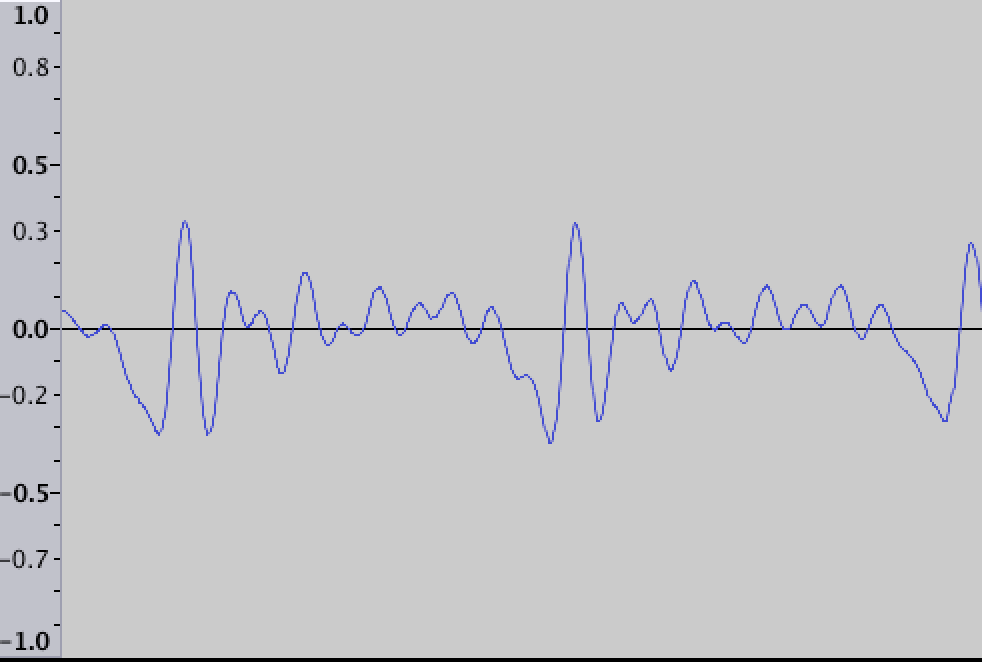
\includegraphics[width=.9\linewidth]{figs/waveform-zoomin.png}
    \caption{When zoomed-in, the frequency information is visible}
    \label{fig:waveform-zoomin}
  \end{subfigure}%
  \begin{subfigure}{.5\textwidth}
    \centering
    
\includegraphics[width=.9\linewidth]{figs/waveform-zoomout.png}
    \caption{When zoomed-out, the frequency information is lost and only the amplitude profile is visible}
    \label{fig:waveform-zoomout}
  \end{subfigure}
  \caption{The effect of scaling on waveform frequency information}
  \label{fig:waveforms}
\end{figure}

This amplitude profile can be used to infer some information about the audio content. For example, speech content has
frequent short periods of silence between words, whereas music has few periods of silence. However, in order to be able
to read this information, users must learn what the different profiles of sounds look like.

Many professional engineers and producers have worked with waveforms for most of their career, and have developed the
skills to be able to read waveforms.  However, without frequency content, there is a limit to the amount of information
waveforms can convey.

We searched for studies that considered the performance of waveforms as an interface to audio content. Although X and Y
included waveforms in their studies, the waveforms themselves were not assessed. No studies could be found that
consider the performance of the waveform itself.

\subsection{Spectrogram}

The spectrogram is a visual representation of the spectrum of frequencies in an audio signal over time.  This technique
allows the full frequency content of the audio to be visible to the user. It is a simple mapping that can be easily
understood, and a generic visualisation that can be used for a wide variety of applications.

Unlike waveforms, spectrograms make it easy for the user to see the frequencies that make up the sound, and in what
proportions. When the time axis of spectrograms is rescaled, the frequency information is still visible, so it is much
more robust to scaling than waveforms. This allows a higher density of information at typically-used scales.

The frequency scale in an audio spectrogram is usually presented on a logarithmic or Mel scale to give a better mapping
of frequencies to the perception of pitch. Psuedocolour (see Section~\ref{sec:pseudocolour}) is often used so that the
detail is more visible.

Higher audio frequencies are displayed at the top of the spectrogram, and the energy of the signal is mapped to the
intensity of the colour. Like with waveforms, these corrolate to two of the cross-modal links listed in
Table~\ref{tab:crossmodal}.

Spectrograms are available in most audio editing software, but rarely used by default. As spectrograms are based on a
Fourier analysis, they are more computationally expensive to plot than waveforms, but trivial for modern computers to
generate.

Although spectrograms present the data very clearly, users must still learn how to interpret the information.  
\citet{Zue1986} found that expert users were able to use spectrograms to read the phonemes of speech, but this is
impossible for the average user to achieve.

The spectrogram displays the energy present in each frequency band, however this can make it difficult for the user to
see the overall energy at a given time.

Spectrograms have a wide range of parameters which control how the data is displayed, including window size and 
shape, frequency and energy scaling, min/max values and pseudocolour methods. This means that is a great deal of
inconsistency between spectrogram, which can make it difficult for users to move from one to the other.

Understanding spectrograms requires users to have basic knowledge about how audio is composed of multiple frequencies.
They would also benefit from understanding how frequencies interact, such as harmonics.

Can be used to edit frequencies like photoshop \cite{Boogaart2006}

%Pros
%X info rich
%X robust to scaling
%X already available
%X simple and generic visualisation
%X computatonally easy

%Cons
%X more computationally expensive than waveforms
%X must learn what different things look like - hard to map frequencies to info
%(doesn't take into account octaves and harmonics)
%X total energy is unclear
%X users must understand that audio is composed of a spectrum of frequencies
%X multiple parameters needed to control visualisation - inconsistent (e.g. window size, window type, 

Spectrograms provide an information-rich and scalable alternative to waveforms, and they are widely available in most
audio editing software. Despite this, waveforms remain a more popular way of interacting with audio. It is unclear as
to why this is.

\subsection{BBC Radio}

9 national stations with 34m listeners, 40 local stations with 8m listeners, one global station in 29 languages with
269m listeners


\clearpage
\section{Semantic audio analysis}
Semantic audio is the extraction of perceptual attributes from an audio signal, which is used to describe sound in
human-readable terms.

% What is semantic audio?
describe sound in human-readable terms
decomposing acoustic signals into semantic entities
can be applied to semantic user interfaces
extracting and describing the perceptual attributes of sound

For example, it can be
used to distinguish between music and speech \citep{Wieser2014}, show where
different people are speaking \citep{AngueraMiro2012}, and who those people are
\citep{Doddington1985}.

classification

Review of audio information retrieval \citep{Foote1999}, including automatic speech recognition, word spotting, speaker
and music identification, and audio similarity

% classification/tagging
This paper divides audio streams into five classes: silence, noise, pure speech, speech over background sound and
music. Four new features are proposed, including silence ratio, pitch frequency standard deviation, harmonicity ratio
and smooth pitch ratio. \citep{Liang2005}
Survey \citep{Duan2014}

% speech-music discrimination
Comparison of features \citep{Carey1999}
For Swedish Radio \citep{Ericsson2009}
Music detection in TV broadcasts \citep{Seyerlehner2007}

% speech-to-text
General books \citep{Junqua1995,Lee1999a}
Speaker diarization review \citep{AngueraMiro2012}
Speech to text on TV (MGB) \citep{Bell2015}
Speech alignment \citep{Bohac2013}
HMM intro \citep{Rabiner1989}

% speaker diarization
\citep{Tranter2006}

% speaker recognition
Overview \citep{Doddington1985}
Book \citep{Lee1999a}

music segmention for intelligent audio editing \citep{Fazekas2007}

Deep belief networks for feature learning \citep{Hamel2010}
Deep neural networks for learning musical features \citep{Sigtia2014}


%Academic research into audio analysis and audio interfaces tends to concentrate on fully automated systems
%\citep{AngueraMiro2012}, navigation of large audio collections \citep{FontCorbera2010} or navigation interfaces based
%on skimming \citep{Arons1997} and scrolling \citep{Lee2007}. Although there are examples of audio visualization from
%the world of academia, it is much more popular in the context of art \citep{Armitage2012}, with excellent examples such
%as Quayola's Form--Sound--Abstraction\footnote{\url{http://www.quayola.com/work/form-sound-abstraction/}} work.

%This section looks at three areas of literature from which the project will draw upon -- extraction of meaningful audio
%properties, mapping these to a visual representation, and the perceptual links between audition and vision.

% parse audio into semantically meaningful features
% map or group these features into semantically meaningful categories

% feature extraction:
% - Fourier
% - MFCCs
% modeling techniques:
% - machine learning
% - clustering
% - markov models
% - GMMS

% speech/music discrimination
% speech
% - speech onset detection
% - speaker diarization
% - speaker identification
% - automatic speech recognition
%   - topic identification
%   - topic segmentation
% music
% - beat tracking
% - chord estimation
% - key detection

%This section looks at audio features that could be used as part of an audio visualization system. Firstly, two use
%cases that were previously identified as being a common component of radio production are explored, before considering
%methods of generating features for any use case.

%Speech/music discrimination (SMD) is the process of segmenting audio content into parts labelled by the categories
%speech and music. In general, SMD classifiers use a collection of different features. This section lists the ones that
%are used frequently or have recently been found to perform well.

%\paragraph{RMS energy}
%The root mean squared energy can be used also exclusively as an effective SMD classifier, as demonstrated in
%\citep{Ericsson2009} and \citep{Panagiotakis2005}.  Commonly used statistics of RMS include low energy ratio
%\citep{Liang2005,Ericsson2009,Saunders1996,Scheirer1997} and variance \citep{Ericsson2009} (including normalised
%variance \citep{Panagiotakis2005} and delta variance \citep{Carey1999}).

%Low energy ratio (also known as `silent interval frequency' and `energy contour dip') is a measure of the number of RMS
%energy frames that fall below a threshold. It exploits the fact that speech has freqent silent gaps between words,
%wheras music does not. The threshold can be set as a fixed value \citep{Liang2005}, a function of a moving average
%\citep{Ericsson2009} or moving peak value \citep{Saunders1996}.

%Kacprzak and Zi\'{o}\l{}ko recently proposed a modified version of low energy ratio called `minimum energy density'
%\citep{Kacprzak2013}. It is calculated by normalizing over a $\sim$15 second window and finding the minimum of the
%normalization function over a $\sim$1--3 second window. It has similar performance to low energy ratio with a moving
%average threshold, but has fewer parameters to set.

%\paragraph{Zero-crossing rate} is the rate at which a signal crosses the time axis, which is an easy-to-calculate
%measure for the spectral energy distribution. Early work in SMD \citep{Saunders1996} identified that ``speech signals
%produce a marked rise in the ZCR during periods of fricativity occuring at the beginning and end of words'', wheras
%music does not. This causes a bimodality which skews the ZCR distribition, which can be measured using the third
%standardized moment (skewness). The variance of ZCR has also been found to perform well for SMD \citep{Scheirer1997}.

%ZCR also played a significant role in two steps of a five-step classifer \citep{Panagiotakis2005}. During silent
%intervals the number of zero crossings is null, so this was used to detect gaps between speech. The authors also noted
%that ``RMS and ZCR are somewhat correlated for speech signals, while essentially independent for music'', and so the
%product of RMS and ZCR was used for the second classifier.

%A review \citep{Carey1999} of features for SMD found ZCR to perform least well, but did not consider the skewness,
%variance, or probability of null zero-crossings.

%\paragraph{MFCC}
%Mel-frequency cepstral coefficients have long been the workhorse of audio analysis, and they have been successfully
%used in SMD applications \citep{Carey1999,Liang2005,Pikrakis2008,Pikrakis2006a,Sell2014,Wieser2014}.  Notably, their
%use has only been successful when used in combination with strong machine learning systems, indicating that the
%relationship of MFCCs to SMD labels is complex and non-linear. This would make it difficult to map to a visual
%representation.

%\paragraph{Chroma}
%Use of chroma features work on the principle that the spectra of music is aligned to the chromatic scale. Pikrakis et.
%al.  \citep{Pikrakis2006,Pikrakis2008} have successfully used `chromatic entropy' for SMD applications. It takes
%sub-bands from a mel-scaled spectrum, aligned to the chromatic scale, and calculates the entropy of the normalised
%spectral energy.

%More recently, Sell \citep{Sell2014} has proposed two new chroma features, which try to account for the fact that the
%chromagram varies greatly between different pieces of music. Music tends to form strong, separated peaks on the
%chromagram wheras speech has smoother mounds of energy. The new features attempt to measure the peakiness of the
%chromagram. `Chromatic diff' subtracts a shifted chroma vector from the original chroma vector and sums the energy.
%`Chroma high freq' performs an FFT on the chromagram and sums the high frequency energy.

%\paragraph{Continuous frequency activation}
%Most of the above SMD features work well for segmenting speech-only/music-only content. However, many fall down at
%detecting background music in speech.  Seyerlehner developed the continuous frequency activation (CFA) feature
%\citep{Seyerlehner2007}, which works on the basis that music content has stable harmonics, seen as horizontal lines on
%a spectrogram.

%A moving average is subtracted from the FFT before it is binarized using a low threshold value. For each bin, the
%proportion of active frames in an analysis window is counted. The result is analysed with a peak picking algorithm and
%the sum of the five largest peaks are used as the CFA. The result is a single numeric value which quantifies the
%presence of steady frequency components.

%In the original CFA paper, the feature was used to find music in television content, but recently it has also been
%successfully applied to segmentaton of radio recordings \citep{Wieser2014}.

%Speaker diarization is the process of segmenting a speech recording by where different people are talking. Review
%papers from 2006 \citep{Tranter2006} and 2012 \citep{AngueraMiro2012} show that the vast majority of systems are based
%on clustering of MFCC or PLP features, which are low-dimensional representations of speech. Rather than developing new
%features, the research is primarily focussed on improvement of the clustering algorithms and pre-processing stages such
%as Wiener filtering, speech activity detection and beamforming.

%MFCC and PLP features are extremely effective when used in machine-based classification systems, but from a human
%perception angle, the features do not correlate well to what is heard.  Other features developed for automatic speech
%recognition may also be useful in a speaker diarization system. For example, spectral entropy \citep{Misra2004} is a
%measure of the peakiness of the spectrum and is an effective feature in distinguishing between voiced and unvoiced
%speech.

%Friendland et. al. \citep{Friedland2009} proposed enhancing the standard MFCC features with a set of long-term features
%representing prosody (the rhythm and intonation of speech). 52 candidate features were ranked using feature selection,
%which showed that ``the median and mean fundamental frequency are the best features, following by high formants (F4,
%F5)''. Inclusion of the top ten prosodic features improved the speaker diarization system by 24\%.

%Traditionally, audio features were developed by hand for specific tasks. This was usually done by attempting to write
%an algorithm that calculated the properties of the sound that humans used to distinuish the categories in question.
%More recently, fuelled by an ever-increasing availability of computing power, research has had a much greater focus on
%automating this process.

%\paragraph{Feature selection/extraction}
%Feature selection and extraction are methods of reducing the dimensionality of a feature vector, either by choosing a
%combination of vector components that best describe the content (selection), or by translating the feature vector to a
%smaller vector while retaining as much information as possible (extraction).

%This process can be unsupervised where only the feature data is known (such as with principal component analysis), or
%supervised where the feature data has corresponding labels (such as with linear discriminant analysis).

%Canonical correaltion analysis (CCA) has been used to reduce the dimensions of features for speaker diarization
%\citep{Chaudhuri2009} and phonetic labelling \citep{Arora2014}, amongst other things. It is able to efficiently map
%features to a subspace and can be used with the kernel trick (known as KCCA) to support non-linear mappings. In the
%case of speaker clustering, ``CCA-based algorithms consistently provide better performance than standard PCA-based
%clustering methods'' \citep{Chaudhuri2009}.

%\paragraph{Feature learning}
%The above methods of reducing dimensionality are based on a relatively short information-rich feature vector that it
%suitable for the target application.  More recent research on feature development is focussed on automated learning of
%features using large labelled datasets.

%Deep learning is an increasingly popular method of learning features based on neural networks with large numbers (tens
%or hundreds) of hidden units. This line of research has been enabled by the increasing availability of large amount of
%processing power. When done properly, deep learning can produce the state-of-the-art in audio features, outperforming
%even the best hand-crafted features \citep{Hamel2010,Sigtia2014}.

%Such an approach requires a high-quality and very large labelled dataset, on which the success of the process depends.
%The nature of neural networks means that it is very difficult to interpret what the resulting features represent which
%isn't an issue when used as the input to a machine learning system, but would make it very difficult to map to a
%visualization. The objective of the deep learning process is to minimise a cost function rather than to maximise the
%link to human perception.

\clearpage
\section{Audio visualization}
Audio visualization is the task of mapping an audio signal to an image. The human visual system is capable of viewing
an entire image at once, and is adept at searching and skimming images. On the other hand, sound must be
consumed serially and over a period of time. Mapping sound to vision allows temporal information to be displayed
spatially, which can overcome some of the limitations of a time-based medium like sound.

We saw in Section~\ref{sec:background-daw} that audio visualization is already used in DAWs to help users navigate and
edit audio content.  However, we also saw that current audio visualizations are limited in what they can display.  For
example, waveforms only display amplitude information, much of which cannot be seen at typical zoom levels.  To
effectively navigate audio waveforms, users must interpret the shape of the visualization to infer whether it is what
they are looking for.  Although in many cases this can be learned, it requires cognitive load to process the images
into the desired information. It also means that novice users must be trained or gain sufficient experience to be able
to reach satisfactory performance levels.
%Audio visualizations can help overcome the contraints of having to consume audio content serially and in real-time.
%Most existing tools treat audio as a collection of digital samples, without much regard for the information contained
%in the audio.

Previous research has proposed a number of enhancements to current audio visualizations that aim to improve their
performance, such as by mapping semantic audio features to colour.  In this section, we start by looking at the
relationship between sound and vision, and considering the perceptual mappings between the two that already exist. We
then review techniques that have been previously used to process or enhance waveforms and spectrograms to make it
easier for users to navigate and edit audio recordings.

%Semantic audio is the extraction of meaning from audio. Example applications of semantic audio are speech-to-text or
%music identification. This technology allows the computer to interpret the audio on the user's behalf in a way that is
%helpful for their situation, however the success of this is dependent on the performance of the audio analysis
%algorithm.

%Semantic audio visualisation is a two-stage process where the audio is first analysed to extract the semantic data,
%then the data is visualised. There are thousands of audio extraction and data visualisation techniques that could
%be combined to create various audio visualisations. The interaction of these two parts, and the context of the
%application, is important in the sucess of semantic audio visualisation. 

%Visual systems can be used to complement audio interfaces, as they are able to address the key challenges of sound.

%In modern society, screens for displaying visual content are widely available.

%Sonic Visualiser from \citet{Cannam2010} can be used to generate these visualisations.


%In a world of `big data', data visualization is becoming an increasing popular subject. Visualization techniques have
%been applied to audio content for a
%variety of applications including accessibility \citep{Ho-Ching2003}, browsing
%large databases \citep{FontCorbera2010}, browsing small databases \citep{Yoo2011} and musical training
%\citep{Ferguson2005} amonst others.

%The development of good visualizations lies somewhere between science and art.
%Tufte's seminal work on good practice \citep{Tufte2001} gives solid guidance on
%creating elegent and unbiased visuals, and Wolfe and Horowitz \citep{Wolfe2004}
%tell us which properties of vision are most critical for visual search.
%However, putting these together in the context of audio requires a certain
%amount of creativity.

%This project focusses on `visualization of time-oriented data', a good overview
%of which can be found in a Springer book of the same name \citep{Aigner2011}.
%The rest of this section will look at examples of time-oriented visualization
%of audio, grouped by the most common visualization techniques.

\subsection{Crossmodality}
To be able to represent audio visually, we must map auditory properties to visual properties.  When attempting to link
sound and vision, it is desirable to create a mapping that is coherent and makes sense to the user.  By creating an
audio visualisation that ``looks likes it sounds'', it might be possible for users to comprehend the sound without
having to listen to it.

\textit{Crossmodal perception} is a term used to describe interaction between the different senses.  Previous work has
shown that there are perceptual mappings between auditory and visual stimuli that are experience by most of the
population. These could be exploited to aid the navigation and editing of audio recordings.

\begin{figure}[ht]
\centering
  \centering
  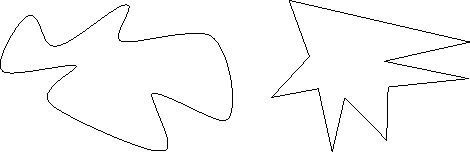
\includegraphics[width=0.8\linewidth]{figs/bouba-kiki.pdf}
  \caption{Demonstration of the ``bouba/kiki effect'', from \citet{Ramachandran2001}}
  \label{fig:boubakiki}
\end{figure}

The ``bouba/kiki effect'' is a demonstration of cross-modal mapping between sound and vision, originally discovered in
an experiment by \citet{Koehler1929}.  Participants were shown two abstract shapes, shown in
Figure~\ref{fig:boubakiki}, and asked to assign the name `bouba' to one, and `kiki' to the other\footnote{K\"ohler used
the words `baluma' and `takete' in the original experiment, but the result was the same.}.  \citet{Ramachandran2001}
found that 95--98\% of the population gave the same answer\footnote{The vast majority of participants chose to name the
sharp, pointy shape on the right `kiki' and the curvy, rounded shape on the left `bouba'.}. This is an example of just
one audio-visual mapping that is common amongst the population.

%\citep{Hubbard1996} did some work to determine which sounds related to which visual properties

%These audio-visual associations are not just higher-level constructs that our
%concious brain creates, they affect the brain at the very lowest level even
%with only brief exposure to bimodal stimuli. Zangenehpour et. al.
%\citep{Zangenehpour2010} used a PET-CT scanner to measure blood flow in the
%brain during exposure to audio and visual stimuli. ``When presented with only
%the auditory or visual components of the bimodal stimuli, na\"{i}ve subjects
%showed only modality-specific cortical activation, as expected.  However,
%subjects who had previously been exposed to the audiovisual stimuli showed
%increased cerebral blood flow in the primary visual cortex when presented with
%sounds alone.''

\begin{table}
\centering
\begin{tabular}{l l}
\hline
\textbf{Link} & \textbf{Direction} \\
\hline
Loudness/brightness  & louder=brighter \\
Pitch/elevation & higher=higher \\
Pitch/size & higher=smaller \\
Loudness/size & louder=bigger \\
Pitch/elevation & higher=higher \\
Pitch/spatial frequency & higher=higher \\
\hline
\end{tabular}
\caption{Audio-visual mappings supported by strong evidence, from \citet{Spence2011}}
\label{tab:crossmodal}
\end{table}

\citet{Spence2011} presented a review of psychology experiments that attempted to find cross-modal links in the human
brain, including audio-visual mapping.  He found that there was strong evidence for six audio-visual mappings, shown in
Table~\ref{tab:crossmodal}.
%There are two common types of test methods used to discover these links -- `speeded' and `unspeeded'.  In `speeded'
%tests, participants are tasked with classifying an audio/visual stimulus and their reaction time is measured. When the
%auditory and visual stimuli are `congruent' (perceived to be similar), then their reaction times are quicker. In
%`unspeeded' tests, visual and audio stimuli are presented very quickly, one after the other, and participants are
%asked to select which stimulus came second. When the stimuli are congruent, participants find it more difficult to
%work out the order of presentation.
These findings were supported by \citet{Tsiros2014}, who attempted to generate images to match different sounds and
measured their success through a user study. In addition to finding strong links between loudness/size and
pitch/elevation, he found weaker links for pitch/colour, dissonance/granularity, and dissonance/colour complexity.

%used a different approach to measure audio-visual crossmodality by using audio visualization
%techniques.  Three audio recordings were used -- a violin, recording of wind noise and impact sound event. For each,
%images were manually created which used different combinations of audio-visual mappings (e.g. dissonance $\to$ texture
%granularity). Participants were played an audio clip and shown an image and were asked whether they are similar or not,
%and to what degree (on a scale of 0--100).

%Tsiros confirms the results revealed by previous studies [7], [15], [19] which found strong relationships between the
%audio-visual feature associations of size – loudness, pitch – vertical position, and weaker relationships between
%color – pitch, texture granularity – sound dissonance and color complexity- sound dissonance

%Additional work from \citet{Marks2003} suggests that cross-modal interaction is a result of late-stage cognitive
%processes.

%Artwork that used synaesthesic style mapping for music to colour \citep{Armitage2012}

%Relationship between pitch and colour \citep{Datteri2004}

%Cross-modality can even be measured in the visual cortex using a PET scanner \citep{Zangenehpour2010}

%Vision and audition are physiologically separate, but idential in many respects
%\citep{Tsiros2013}.

Current audio visualizations exploit some of these cross-modal mappings. For example, waveforms map loudness to size,
and spectrograms map loudness to brightness, and pitch to elevation. However, this previous work shows that there are
many more links between sound and vision that have yet to be fully exploited by audio visualizations.

\subsection{Waveforms}

The audio waveform is commonly used by most DAWs and other audio software as a visualization of an audio signal.  As
such, users are very familiar with navigating audio content using waveforms, and many have learned how to read the
shapes of the waveform to read useful information about the audio. Enhancing waveform, by either processing it or
adding additional information to it, could allow users to navigate and edit audio content more efficiently whilst
retaining this familiarity and using the skills they have developed.  We identified two main approaches that have been
used to enhance waveforms -- scaling and colour.

\subsubsection{Scaling}
The scale at which a waveform is viewed is crucial to its effectiveness. There are two axes with which the scale is
controlled using horizontal and vertical zoom.  Horizontal zoom adjusts the time period that is viewed, which affects
the visibility of the frequency information.  Vertical zoom adjusts the amplitude range that is viewed, which affects
the visibility of the amplitude profile.

One very simple technique for improving waveform readability is to automatically scale the vertical zoom to match what
is visible on the horizontal timeline.  However, if the scale of the waveform constanstly shifts, there is no reference
level by which to compare the amplitude of the audio.  The solution proposed by \citet[p. 39]{Goudeseune2012} was to
overlaying a dimmed version of the scaled waveform on top of the normal waveform. This allowed users to simultaneously
judge the level whilst being able to see the detail of the amplitude profile.

Frequency information is useful for understanding the timbre of an audio signal. When viewed at the right scale, this
is visible in a waveform, but at typical horizontal zoom levels, this information is lost. \citet{Loviscach2011}
proposed a novel solution to this problem called the ``quintessence waveform''. This approach used extreme pitch
shifting to preserve the character of the waveform at different scales.  This works well for repeating monoaural sounds
-- for example, a sine wave would be identifiable as a sine wave at every zoom level.  However, typical real-life
applications use complex polyphonic audio, which would not benefit from quintessence waveforms as there is no repeating
signal that could be displayed.

%\begin{figure}[p]
  %\centering
  %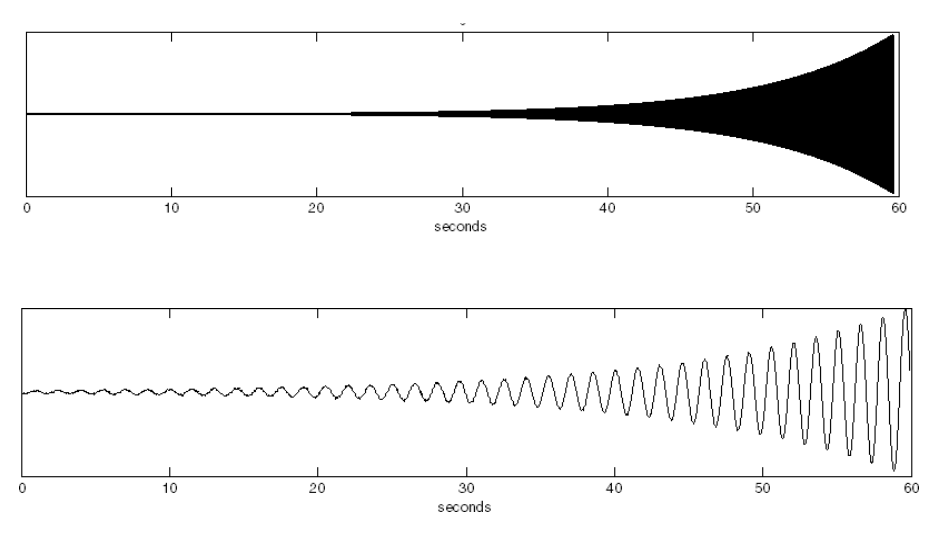
\includegraphics[width=0.95\linewidth]{figs/quint.png}
  %\caption{Above: Normal waveform, below: quintessence waveform, source: \citep{Loviscach2011}}
  %\label{fig:quint}
%\end{figure}

\citet{Gohlke2010} proposed five novel ideas on how to improve multi-track DAW displays, including techniques for
saving screen space by overlaying and stacking waveforms. One of these proposals was for a lens-like view, which
magnified the area of the waveform around the current playhead position. This allowed users to simultaneously view the
waveform at two different scales -- an overview of the audio waveform and a detailed local view. This concept has the
potential to display frequency information in regions of interest, and help make more precise audio edits without
adjusting the overall zoom level.

%waveform tracks can vertically overlap by 25\% without dramatically affecting display quality
%waveforms are mostly symmetrical, so by discarding one half the overlap can be increased to 50\%
%stack graph for contribution of each track to perceived loudness

\subsubsection{Colour}
The use of colour is a simple and effective way of adding additional information to a waveform.  However, many DAWs use
waveform colour to distinguish or label audio clips, and most others have monochromatic waveforms.  Previous research
has experimented with mapping semantic audio features to colour, using either pseudocolour or false colour.

\textit{Pseudocolour} is a method of mapping a scalar value to a colour gradient \citep{Moreland2009}, an example of
which is thermal imaging cameras.  Colour gradients are composed of at least two colours (e.g. blue to red) or a
spectrum of colours (e.g. a rainbow).  Pseudocolour allows values to be mapped to colours that might be perceptually
relevant (e.g. green/red for good/bad).  It can emphasize small variations between values by using a full spectrum,
pick out high/low values using non-linear gradients, or categorize values using stepped gradients.  However, as
pseudocolour can only represent one dimension, it does not make full use of the available colour space.

\textit{False colour} is the mapping of multiple values to the dimensions of a colour space. Commonly, three values are
mapped to red/green/blue (RGB) colour space. Other colour spaces can be used, such as hue, saturation, value (HSV),
which better matches human perception of colour. Hue means colour on a rainbow, saturation means lack of grayness, and
value means brightness. The advantage of this method is that it can make full use of the available colours.  On the
other hand, it can be challenging to select three values and map them to colour in a way that is perceptually relevant
and understandable.

\citet{Rice2005} presented \textit{Comparisonics}, which uses pseudocolour to map the frequency content of an audio
signal to a colour spectrum.  Comparisonics was designed for identifying timbrally distinct sounds and they claim that,
with training, it can be used to identify certain sound effects.  Their technique maps low/mid/high frequencies to
blue/green/red colours, respectively, using an unpublished algorithm.  Comparisonics has since been integrated into the
\textit{Scratch LIVE} DJ software from Serato Audio Research, where it was used to distinguish between different drum
noises, such as bass kicks, snares and high-hats.

A very similar system was implemented in the audio clip sharing website \textit{Freesound} \citep{Akkermans2011} to
help users quickly find and compare sound effects and music clips.  They used pseudocolour to map the ``spectral
centroid'' of the audio to a colour gradient.  Spectral centroid is the weighted mean of the frequencies of a signal
\citep[p. 10]{Smaragdis2009}, so a low value indicates the presence of mostly low-frequency sound and vice-versa.

\citet{Loviscach2011a} used pseudocolour to enhance the navigation of speech. The ``zero-crossing rate'' of the audio
was mapped to a red/green/blue colour spectrum to help distinguish between different phonemes (e.g. ``oo'' or ``s'').
The zero-crossing rate is the frequency with which an audio signal switches between a positive and negative value
\citep[p. 37]{Zhang2010}, which is a crude measure of the primary frequency of the audio.

\citet{Tzanetakis2000} used false colour to create a visualisation technique known as \textit{Timbregrams}. Their aim
was to ``use color perception and the pattern recognition capabilities of the human visual system to depict timbral and
temporal information''.  Their implementation extracted a large vector of common audio features, then used principal
component analysis to reduce the size of the vector whilst retaining 80\% of the variance in their data.  They mapped
the first three principal components of the feature to RGB or HSV colour space.  They found that the RGB colour space
was more uniform and aesthetically pleasing, but that the HSV colour space had better contrast at segmentation
boundaries. When using RGB, speech, classical music and rock could easily be distinguished as they appeared as light
green, dark blue and dark green, respectively. Tibregrams were later used to colour a waveform in a basic audio editor
\citep[p. 253]{Tzanetakis2001}.

\citet{Mason2007} used false colour to assist radio listeners in navigating recently-broadcast material. They mapped
three empirically-chosen audio features to RGB colour space. The authors reported that the system was successful at
indicating the location of music within speech content, and highlighting low-bandwidth material such as phone calls.
The authors proposed that the system could be also be applied to other applications such as segmentation of radio
programmes for re-editing into podcasts.

%\begin{figure}[p]
%\centering
%\begin{subfigure}{\textwidth}
  %\centering
  %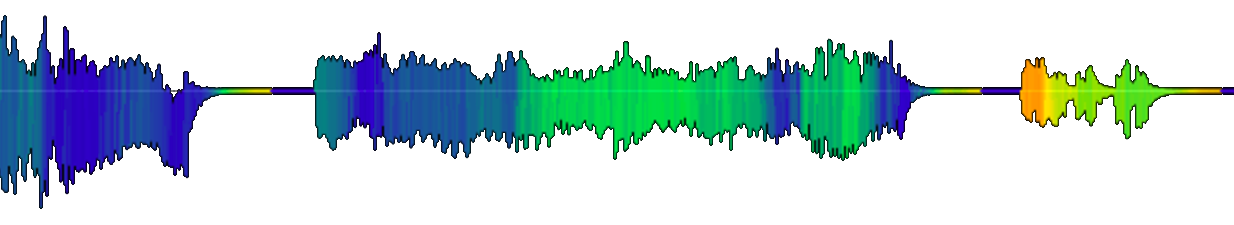
\includegraphics[width=\linewidth]{figs/freesound2.png}
  %\caption{Freesound (\url{freesound.com})}
  %\label{fig:freesound}
%\end{subfigure}\\%
%\begin{subfigure}{\textwidth}
  %\centering
  %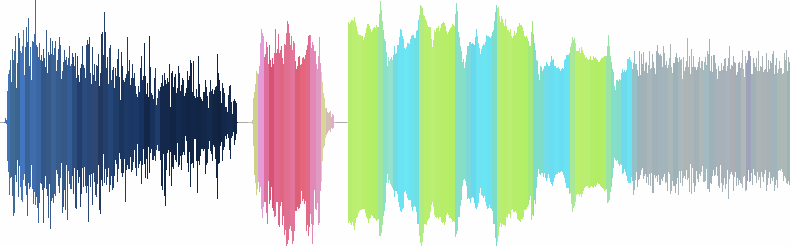
\includegraphics[width=\linewidth]{figs/rice.png}
  %\caption{Comparisonics \citep{Rice2005}}
  %\label{fig:rice}
%\end{subfigure}
%\caption{Examples of pseudocolour (\ref{fig:freesound}) and false colour
  %(\ref{fig:rice}) applied to colourising an audio waveform}
%\label{fig:colourvis}
%\end{figure}

%False colour has also been used for navigating and summarizing extremely long recordings. \citet{Towsey2014} mapped
%three spectral features to RGB colour for visualizing almost a year of environmental recording.
%Figure~\ref{fig:towsey} shows the recordings from March until October, with each line representing one day.  The
%visualization reveals the change in time of the dawn and evening choruses throughout the year, amongst other things.

%\begin{figure}[p]
  %\centering
  %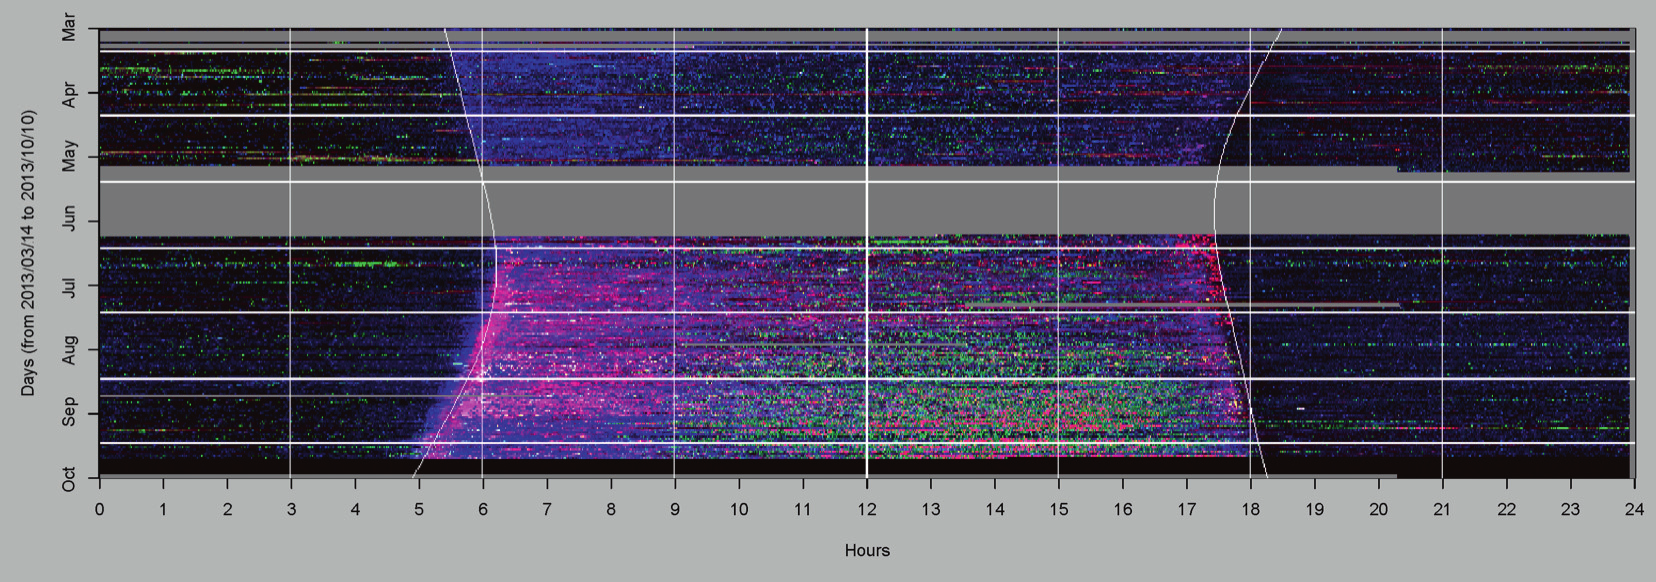
\includegraphics[width=0.95\linewidth]{figs/towsey.png}
  %\caption{False colour visualization of environmental recordings, with each line representing one day. Missing data is
    %shown in grey.
    %\citep{Towsey2014}}
  %\label{fig:towsey}
%\end{figure}

\subsection{Spectrograms}

Spectrograms display the amplitude of audio frequency over time. Unlike waveforms, the frequency information is visible
at all zoom levels, which makes them much more robust. They display so much information that, with sufficient training,
it is possible to read speech using a spectrogram \citep{Zue1979,Zue1986}.  However, despite these advantages, audio
waveforms are much more widely used than spectrograms in audio production.

%\citet{Gohlke2010} proposed a
%thresholded spectrogram overlaid with different colours for each track to minimuse spectrotemporal overlap and masking

\citet{Lin2012} introduced a method of filtering spectrograms to visually emphasize non-speech events in long audio
recordings. The filtering was done using an ``image saliency algorithm'' that detected differences in the intensity and
orientation of the spectrogram image. This \textit{saliency-maximized spectrogram} was integrated into an audio
navigation interface called \textit{Timeliner} \citep{Goudeseune2012}, which displayed the spectrogram alongside a
waveform. \citet{Lin2013} describes an evaluation in which 12 novice participants used Timeliner to find sound effects
hidden in meeting room recordings using both saliency-maximized and normal spectrograms. The results show that
saliency-maximized spectrograms significantly outperformed normal spectograms.
Filtering spectrograms shows promise as a way of detecting unusual events, however it is unclear how useful this sort
of application would be in the context of radio production.
%A user study of Timeliner for audio event detection \citep{Hasegawa-Johnson2011} Uses false colour to map min, mean
%and max values to the HSV colour space

%\begin{figure}[ht]
  %\centering
  %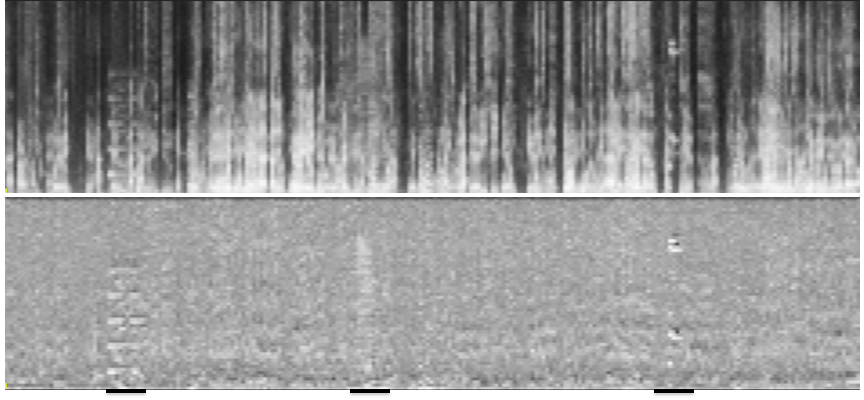
\includegraphics[width=0.95\linewidth]{figs/spectrogram-salience.png}
  %\caption{Top: A normal spectrogram; Bottom: A salience-maximised spectrogram with target events marked using black
    %underlines}
  %\label{fig:timeliner}
%\end{figure}


% Could use image synthesis \citep{Levkowitz1991}

\clearpage
\section{Speech segmentation}

Waveforms and spectrograms provide a direct mapping of sound to vision, which is then interpreted by the user. The
benefit of this approach is that it can be used for a wide variety of tasks with any type of content.  The downside is
that the user must learn how to read these visualizations, and view them at an appropriate scale.

With many audio recordings, the content can be divided into logical groupings that could help the user navigate the
recording. For example, a ``magazine-style'' radio programme is made up of several pieces on different topics. Being
able to view what those topics were, and where they occured in the programme, would assist listeners in navigating to
a topic of interest.

Semantic audio analysis techniques have been widely used to classify and segment audio into a range of logical
categories. These are often combined with data visualization techniques \citep{Aigner2011} to create novel user
interfaces that aid the navigation and editing of audio content.

We have divided these segmentation techniques into two broad categories: classification, where audio is segmented by
the character of the audio (speech, music etc.), and topic summarization, where the audio is segmented by its content.

\subsection{Classification}

Audio can be divided into human-readable segments using semantic audio analysis techniques.  Semantic audio analysis
typically operates in two main steps: dividing an audio file into sematically meaningful segments, then grouping these
segments into semantically meaningful categories \citep{Lu2009,Zhang2010}. These categories can be chosen to match the
application being targeted. For example, a radio broadcast might be divided into speech, music, speech mixed with music
and applause.

This semantic audio segmentation has applications to audio editing \cite{Avdelidis2007}.

\subsubsection{Speech/music discrimination}
Speech-music discrimination (SMD) is the task of segmenting an audio recording and labelling those segments as either
speech or music.
Previous research into automated SMD has often targeted recordings of radio broadcasts
\citep{Goodwin2004,Wieser2014,Saunders1996,Pikrakis2008,Pikrakis2006a}.
%Clustering is a task in which comes naturally to humans, but machines often struggle with.




\subsubsection{Speaker diarization and identification}
\textit{Speaker diarization} is the task of segmenting a speech recording according to speaker identity, which is used
to answer the question ``who spoke when?'' \citep{AngueraMiro2012}. Segments are given a unique label for each speaker,
but the identity of the speakers is unknown.  \textit{Speaker identification} is the task of identifying the person who
is speaking based on the sound of their voice.

\citet{Raimond2014} introduced the \textit{BBC World Service Archive prototype}, which was an interface that used
automatic keyword tagging and crowd-sourcing to support the search and discovery of a large radio archive.
The interface used speaker diarization and speaker identification to help users navigate within individual radio
programmes. Figure~\ref{fig:bg-world-service-archive} shows an example of a radio programme that has been segmented
into five named speakers.

\begin{figure}[ht]
  \centering
  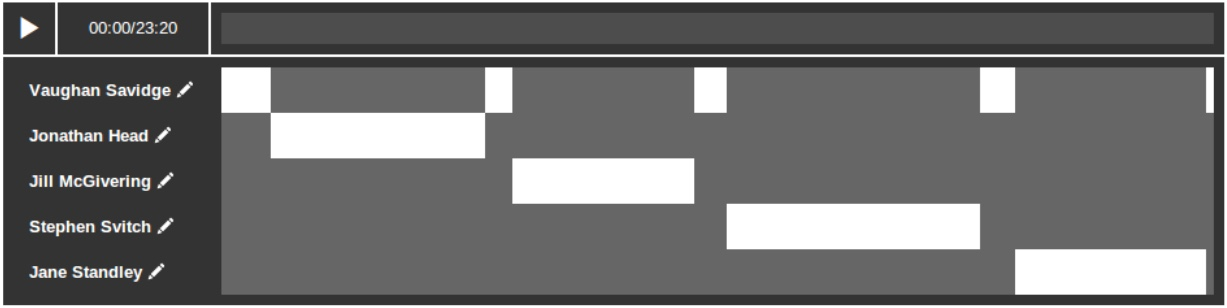
\includegraphics[width=\linewidth]{figs/world-service-archive.jpg}
  \caption{Speaker diarization and identification interface in the BBC World Service Archive prototype, from
  \citet{Raimond2014}}
  \label{fig:bg-world-service-archive}
\end{figure}

%Speaker identification with crowd-sourcing achieved 85\% precision and a 43\% recall

which used speaker diarization and
identification to facilitate navigation of radio programmes. The prototype relied on crowd-sourcing to add the speaker
names, which then populated a central database of speaker identities.

Segmentation algorithms often use a threshold value to configure their sensitivity. In the case of speaker diarization,
a low threshold would increase the recall and reduce the precision. For example, more speaker turns would be detected,
but some may be incorrect.  This threshold is often set to minimise a cost function, which balances the precision and
recall.  \citet{Foote1998} describes a video browser prototype that allowed the user to control this threshold value,
using a slider in the user interface. Their prototype identified speaker turns, but did not attempt to match the
identities of the speakers.



% TOPIC SEGMENTATION
\subsection{Topic summarization}

Topic summarization has previously been used to assist the discovery and search of media archives \citep{Raimond2014,
Kim2003}. However, the same techniques can also be applied to aiding the navigation of audio files using segmentation.

% can use text summarization
Text summarization review paper \citep{Lloret2012}

% video digests
Video digests divide video recordings into chapters, sections and summaries.
\citet{Pavel2014} describes an interface for writing and editing video digests

% segmentation with keywords 
\citet{Abdulhamid2013,Abdulhamid2013a} introduced \textit{SpEx}, which is an interface designed to help students
navigate lecture recordings.

World service archive \citep{Raimond2014} topic extraction


% OTHER

% repeated bits
Similarity matrix can be used to discover and display repeated regions of audio \citep[p. 6]{Cooper2006}

% text
Text segmentation \citep{Choi2000}

% (below not relevant)
%Evaluation of SpeechBot for searching radio archives \citep{Kim2003}

\clearpage
\section{Textual representation}\label{sec:background-transcripts}

Writing is widely used to record speech, in a process known as ``transcription''. Transcripts can be used to record
exactly what somebody said, and the transcript text can be read, copied, shared, skimmed and searched using a variety
of tools, such as word processors, or on paper.  \citet[p.~133]{Hausman2012} notes that radio producers currently
``cut, paste and copy sound files much the same way we use a word processor to manipulate words, sentences and
paragraphs''.  In this section, we will see how transcripts can be used as an interface to aid the navigation and
editing of speech recordings.

% transcripts can increase the navigation speed
\subsubsection{Transcript generation}
Transcript are often written manually, either using pen and paper or a word processor. Based on the author's informal
discussions with radio producers, it can take them between 2 and 5 times the length of recording to transcribe
the speech, and is a slow and tedious process. Producers can save time by only transcribing the most salient words, but
this makes the transcript much less readable, particularly to others who haven't heard the original recording.
Alternatively, producers can use a third-party to transcribe the speech on their behalf, but this slow and expensive.
For example \texttt{rev.com} charges \$1 per minute for a 12-hour
turnaround\footnote{\url{https://www.rev.com/transcription}, accessed 11/12/2017}.

% two types: manually written (perfect, but expensive and slow) or automatic (erroneous, but fast and cheap)
% comparison?
Automatic speech recognition \citep{Junqua1995}, known as ``ASR'', can be used to convert speech to text.  ASR is
quicker and cheaper than manual transcription.  ASR also produces accurate timestamps for each word, which can be used
to precisely navigate and edit the audio, but word-level timestamps can also be added to manually-written transcripts
using speech alignment \citep{Griggs2007,Bohac2013}.  ASR transcripts don't include letter capitalization or
punctuation, but this can be estimated and added using post-processing.

Despite advances in the field \citep{Lee1999a}, ASR produces erroneous transcripts.  \citet{Bell2015} conducted an
evaluation of ASR systems on television programmes of various genres. Each system was judged by the proportion of
incorrect words, known as the ``word error rate'' (WER).  The mean average WER of the systems tested was 23.7\%,
however the variance across the programmes was high, with the WER varying from 10-–41\% across the 16 programmes.
Erroneous transcripts reduce listener comprehension \citep{Stark2000,Vemuri2004} and increase the time it takes to
search audio content \citep{Ranjan2006} and correct errors \citep{Burke2006}.  However, despite these errors, ASR
transcripts provide a highly effective tool for browsing audio content as users can visually scan the text to focus on
regions of interest, known as ``strategic fixation'' \citep{Whittaker2007}.

%\citet{Vemuri2004} conducted a user study of 34 participants and measured their comprehension of short audio clips when
%presented with both perfect and auto-generated transcripts.  The results show that subject comprehension of audio
%presented with a perfect transcript (C1) was found to be better than an automatically-generated transcript.
%completely wrong transcripts aren't worse than no transcript

%\citet{Ranjan2006} studied the performance of 13 participants in an audio search task with varying levels of
%transcript quality. The results showed that the mean search time descreased as the transcript quality increased.

%\citet{Burke2006} found that higher quality transcripts required users to listen less to complete a correction task.

%Automatic speech recognition technology makes it possible to extract partially accurate transcripts of speech
%recordings.  A number of researchers have experimented with using these transcripts to enhance interfaces for
%interacting with audio content.
%\subsection{Navigation}

% navigation with transcripts

\subsection{Transcript navigation}
Transcripts have previously been used by several systems as an interface for improving the navigation of speech-based
content such as news reports and voicemail messages. 
One of the first such systems was \textit{NewsTime} from \citet{Horner1993}, which used transcripts to aid the
navigation of audio news stories.  For television news, closed captioning was aligned the audio to provide an accurate
transcript with word timings.  NewsTime included several additional features including searching by keyword, segmenting
the transcript by story and speaker, jumping to the next or previous speaker/story, and categorizing stories into one
of seven common topics. There were no reported user studies of NewsTime.

\textit{SCAN} \citep{Whittaker1999} was an interface designed to support retrieval from speech archives. It used ASR transcripts
to allow users to search for keywords and visually search the recording by reading the transcript.  In a user study of
12 participants, the transcript was found to support navigation by reducing the listening time needed to complete
information retrival tasks. Participants rated the transcript as easier and more useful with the transcript than
without.  SCAN was further developed into \textit{SCANMail} \citep{Whittaker2002}, an interface designed for interacting with
voicemail.  It added a number of features including paragraph segmentation and the ability to seek to a point in the
audio recording by clicking on a word in the transcript. The results of a user study of eight expert users showed that
the transcript display enabled users to visually scan the content of recordings to quickly extract information and
judge which parts were relevant, without having to play the audio.
%SCANMail did not include editing capabilities

\subsection{Semantic speech editing}
In addition to supporting the navigation of speech recordings, transcripts have also been used as a method of editing
speech content. The first of these was the `Large Interactive Display System Wave Speech Editor', or
\textit{LIDSWSEdit}, from \citet{Apperley2002}, which used ASR transcripts to allow users to navigate and edit lecture
recordings.  Any edits made to the transcript were correspondingly applied to the underlying audio recording, known as
``semantic speech editing''. Users could re-arrange sentences and words by selecting the text, then using a
drag-and-drop action.  Alternatively, speech could be removed by selecting text then clicking a button to either delete
the selected text, or everything except the selected text.  LIDSWSEdit was further developed into the
`TRanscription-based Audio EDitor', or \textit{TRAED} \citep{Masoodian2006}.  TRAED used the same editing actions as
LIDSWSEdit, but rather than displaying the text and audio waveform separately, it displayed the waveform in-line with
the text. Individual words were indicated by drawing boxes around the waveform and word. The boundary between each word
pair could be adjusted by dragging the boundary edge.  We could not find any user studies of LIDSWSEdit or TRAED.

\citet{Whittaker2004} created an interface for editing voicemail messages using ASR transcripts.  Users could
cut-and-paste parts that they wanted and delete other parts.  The system was evaluated in a formal study of 16
voicemail users, which found that semantic editing was faster and as accurate as editing with a waveform-based
interface. Crucially, this was true even though the transcripts had an average word error rate of 28\%. This
demonstrates that semantic editing is beneficial even when using erroneous transcripts.

\citet{Rubin2013,Rubin2015} presented a novel interface for creating ``audio stories'' that, similarly to radio
programmes, combine speech and music.  The interface used an editable transcript with two columns, one for each of a
pair of speakers.  It allowed the user to cut, copy, paste and delete the audio using the text. It also highlighted
repeated words, similar sentences, ``umm''s, breaths and pauses in the transcript. The transcripts were generated using
a crowd-sourcing service with speech alignment software that also detected breaths.  The system also included
additional functionality for finding and adding music tracks, and for varying the length of music using automatic
looping. The system was evaluated through a short informal study of four participants where the editing capabilities
received positive feedback. No follow-up studies have been reported since.

\citet{Sivaraman2016} created a semantic editing system for asynchronous voice-based discussions, where users could
quickly edit their speech recording before sending it to the recipient.  Their system used near-live automatic
transcription and detected pauses in the speech. Their interface allowed users to delete selected words/pauses, insert
additional pauses and fix incorrect words.  In a formal qualitative study of their system with nine users, they found
that text-based editing was considered good enough to replace waveform editing, and to be more accessible. They
observed that most users only used the system to make fine-grained edits, instead of editing large chunks.  Users said
that the transcript also allowed them to quickly review all the points that were made, and that the errors in the
transcript weren't a heavy distraction. A quantiative study of 28 students and teachers found that
including editing functionality resulted in the students reporting lower levels of mental task load, effort and
temporal demand.

\citet{Yoon2014} created a collaborative tablet-based document annotation system called \textit{RichReview}, which
offered users three modalities in which to annotate documents - freeform inking, voice recording and deictic gestures
(i.e. pointing to areas of interest). The voice recordings were displayed using a waveform, overlaid with an ASR
transcript of the speech.  Users could trim or tidy the voice recordings by drawing a line through words or pauses to
remove them.  The system was evaluated using a qualitative study of 12 students which found that the editing features
were considered easy to use and efficient for removing ``umm''s and long pauses.  However many participants reported
that the transcripts were not accurate enough to use without having to listen to the audio.
%RichReview was later deployed as a web applet on the online education platform edX \citep{Yoon2015a}.
\citet{Yoon2016} describes two deployment studies that used a similar system called RichReview\textsuperscript{++}, but
this did not include any semantic editing functionality.

\subsection{Video editing}
Semantic speech editing has also been used to support video editing.  \textit{SILVER} \citep{Casares2002, Long2003} was
a video editor that aligned words from closed captions to the video.  Gaps, errors and edits were displayed in the
transcript using special characters.  The video could be edited by deleting text in the transcript.  SILVER was
evaluated in an informal study with seven students, but the study did not report any results about the transcript-based
editing feature.

Hyperaudio Pad is an open-source audio and video editor, first proposed by \citet{Boas2011}, and now available online
as a free service \citep{Hyperaudio2016}. This is a web-based interface that allows users to navigate and edit online
media using transcripts. The transcripts are generated from subtitles by using speech alignment software. Editing is
done by selecting a part of the transcript and dragging it into a window to create a `clip'.  Other clips can be added
and re-ordered, and the edited version can be played and shared with others. No user studies of this system could be
found.

% video editing using perfect transcripts
When editing a video interview, you want to avoid making a cut when the person speaking is in shot, because it causes
the image to suddenly jump.  \citet{Berthouzoz2012} used image processing algorithms to create a video editor that can
help the user hide these edit points. The editor had an editable transcript window that displayed suitable edit points
and allowed the user to edit the video by selecting and deleting text. The transcripts were generated manually using an
online crowd-sourcing service, and word timings were added using speech alignment software. The system also allowed
users to easily remove `umm's or repeated words as they were explictly marked in the manual transcript. No user study
was conducted in the reported study, however positive feedback was received from nine professionals who were given a
demonstration.

\subsection{Pre-written scripts}
The systems so far have only considered transcripts that have been generated from the speech itself. However, sometimes
speech is recorded based on a pre-written script, or from notes.  Avid released a feature for their Media Composer
video editing software in 2007 called \textit{ScriptSync} \citep{Avid2011}.  This feature aligns a user-supplied
transcript to a video recording by placing a marker in the video for each line of the transcript \citep{Griggs2007},
allowing users to jump to a particular line, or see which line in the transcript corresponds to the current point in
the video.  A second version of ScriptSync was launched in February 2017 \citep{Avid2017} which added script correction
and collaborative note-taking.
%We did not find any reported user studies of ScriptSync.

\citet{Shin2016} created a system called \textit{Voice Script} that supports an integrated workflow for writing
scripts, and recording/editing audio. An informal study with four amateur participants found that it could support
various workflows including multiple iterations. It included a `master script' layout which was used to bring together
different recordings,  and that was found to work well.  A second study of four amateur participants directly compared
the system to that of \citet{Rubin2013}, which found that participants were able to complete an audio production task
25\% faster using the Voice Script system.  This study demonstrates that for workflows that involve pre-written
scripts, there is potential to improve the audio editing by using an integrated writing and editing system.

\textit{QuickCut} from \citet{Truong2016} was an interface designed to help producers edit a narrated video from a
pre-written script, voiceover audio and raw video footage.  Producers could label their video footage using their
voice, which was manually transcribed using a crowd-sourced online service. Speech alignment was used to align the
script to the voiceover audio.  Selecting text in the script also selected the corresponding segment in the voiceover
audio, and displayed video clips that were labelled with similar words. After selecting an appropriate clip, it could
be added to the timeline using drag-and-drop to associate it with a position in the script.  The completed timeline
could then be exported as and ``edit decision list'' (EDL) for use in professional video editing software.  QuickCut
was evaluated by the researchers themselves and one professional filmmaker, who were able to use the system to produce
videos in a fraction of the time normally needed.  Voice-based logging makes sense for logging video footage as it is
easy to watch and talk at the same time. However, for speech content it would be difficult to talk and listen
simultaneously.  The ability to export edits to professional software allows for a smooth continuation of the
production workflow.

%ellipses were used to indicate pauses.
%three constraints - alignment, alternative, ordered

% CORRECTION

\subsection{Transcript correction}
SILVER \citep{Casares2002, Long2003} 

\citep{Masoodian2006} included correction by selecting a word and typing a replacement. New spaces created a new word,
dividing the time in half.

\citet{Burke2006} added correction functionality to the SCANMail interface by allowing users to either select a
replacement word from a drop-down menu, or select multiple words and type over them. A user study of 16 participants
correcting voicemail messages showed that the menu interface required much less listening than typing.

\citet{Liang2014} showed that once an incorrect word is identified, in 30\% of cases the correct word can
automatically be inferred using $n$-grams and acoustic features.

Normally, correction is a post-production process that can take up valuable time, although as \citet{Wald2007} shows,
real-time correction of speech is feasible.

\citep{Suhm2001}

%TypeTalker - editing spoken comments \citep{Arawjo2017}
\textit{TypeTalker} from \citet{Arawjo2017} was an interface for editing synthesized speech comments using ASR
transcripts. The speech was synthesized from recordings of the user's comments, which was done to reduce their
self-consciousness. As well as being able to remove unwanted speech, the use of speech synthesis meant that new speech
could be inserted and words could be changed.

%Colour, size and orientation guide visual attention for visual search \citep{Wolfe2004}

% confidence shading
\subsection{Confidence shading}
In addition to producing a transcript, many automatic speech recognition systems return a confidence score for each
transcibed word, indicating how sure the system is that the word is correct. ``Confidence shading'' is a technique for
displaying this score by colouring words with a low confidence score in a lighter shade.
Confidence shading has been used in an attempt to make mistakes easier to locate, and transcripts easier to read.
%It is hypothesised that confidence shading makes it easier to identify incorrect words for the purposes of correction,
%and increases the comprehension of the text because the lighter shade makes mistakes less apparent.
Confidence scores may themselves be incorrect by indicating false positives (when a correct word is marked as
incorrect), or false negatives (when an incorrect word is missed). The balance between the two is controlled using the
threshold value between 0 and 1. As \citet{Feng2004} demonstrates, a higher value reduces false positives and increases
false negatives, while a lower value increases false positives and reduces false negatives.

\citet{Suhm2001} conducted a user study of 15 participants who corrected an ASR transcript with and without confidence
shading (in this case, highlighting). The results showed that correction with confidence shading took slightly longer
than without, although this was not statistically significant.  Conversely, \citet{Burke2006} reported that users find
confidence shading helpful. 16 participants performed a transcript correction task with confidence shading and overall
they agreed that shading was helpful for identifying mistakes.  One notable difference between these studies is that
\citet{Suhm2001} optimised their confidence threshold to minimise the overall accuracy of the confidence shading, whilst
\citet{Burke2006} increased the threshold to treat false negatives more seriously.

\citet{Vemuri2004} studied whether confidence shading improved comprehension of the transcript. They conducted a user
study of 34 participants and measured the comprehension of short audio clips when using ASR
transcripts with and without confidence shading. Although the results indicated better comprehension with confidence
shading, there was no statistically significant difference.

\subsection{Keyword extraction}

Keyword extraction \citep{Matsuo2004}

Keywords used by \citet{Loviscach2011a} as part of his nimble video editor

% keyphrases from speech, using ASR, poor quality
Extracting keyphrases \citep{Inkpen2004}


%TODO other applications
%Coding of video interviews \cite{Chandrasegaran2017}

%VisScribe - interactive transcript interface and speaker activity for coding design sessions \cite{Chandrasegaran2017}

%Personal device for recording and navigating notes using keywords \citep{Tucker2003}

\clearpage
\section{Audio playback interfaces}

The previous work we have considered so far have used rich visualizations to display complex representations of
transcripts, speakers, structure and summarizations. Visual presentation of audio content makes it easier for users to
search and skim the information, but it is difficult, if not impossible, for humans to fully comprehend sound using
visual means. Listening is the natural way for humans to consume audio content, but the time required to listen can
make it a lengthy and inefficient process.

Audio processing can be used to increase the speed at which users can listen to audio recordings. Previous research has
used two main techniques to achieve this. The first uses processing to improve the comprehension of speech at higher
playback rates.  The second exploits the ``cocktail party effect'' by playing multiple audio streams simultaneously and
using audio processing to help the listener separate the sounds.  We discuss each of these techniques below.

\subsection{Time compression}

% problem description
Listening to long audio recordings of speech can be time-consuming. A simple way to reduce the listening time is to
increase the rate of playback.  However, this increase in speed causes an upward shift in the pitch of the sound, which
degrades the speech and makes voices sound like chipmunks. The increased speed with which the content is presented
also makes it difficult for listeners to process the information fast enough.

These limitations negatively affect the intelligibility and comprehension of the speech.  In this context,
\textit{intelligibility} refers to the ability to identify words, and can be measured by the accuracy with which a
specific word is recalled. \textit{Comprehension} refers to the ability to understand the content of the material,
measured by the number of correctly answered questions about the subject matter.

%By carefully selecting which words to listen to, speech
%can remain intelligible at up to 10-times normal speed \citep[p.~7]{Arons1997}.
%TODO better citation needed

% difference between time compression and speech skimming
There are several approaches for reducing the time required to listen to a recording while being able to extract
critical information, which can be divided into two categories. \textit{Speed-up} techniques aim to increase the speed
of playback without affecting the pitch of the speech, and \textit{excision} techniques aim to remove parts of the
speech in a way that minimises the reduction in comprehension.

% speed-up vs excision
\citet{Tucker2006} performed a user study that compared two different excision techniques and a speed-up technique,
using both 5-min and 30-min audio recordings.  Participants ranked a list of utterances to match what they heard, which
was compared to a reference response to produce a score for comprehension. This score was normalised by the listening
time to measure ``comprehension efficiency''.  The results showed that for short recordings, excision outperformed
speed-up, but that they performed similarly for long recordings. However, when using excision, participants were less
likely to switch to normal-speed playback, and they reported that they prefered excision to speed-up.

%time compression and speech skimming.
%\textit{Time compression} refers to a set of sampling techniques that are used to reduce the length of the audio by
%skipping or over-lapping audio frames.  \textit{Speech skimming} exploits the natural boundaries and acoustic
%properties of speech to structure the audio content based on salience. This can be determined based on the location and
%frequency of natural pauses, the emphasis of the voice (usually determined by pitch), speaker diarization and the
%content of the speech.

% time compression (sampling techniques)
% - shortening/removing pauses
% - isochronous sampling (regularly skipping frames)
% - SOLA (overlapping frames)
% - dichotic sampling
% - backward sampling
%
% skimming (structuring the audio by segmenting based on saliency, then skipping)
%   - pauses
%   - pitch-based emphasis
%   - content-based
%   - speaker diarization

% excision techniques
% isochronous sampling, shortening/removing pauses
The simplest excision technique is to remove frames of audio at regular intervals, known as ``isochronous sampling''.
However, this approach does not discriminate between valuable and redundant information. It also fails to take into
account speech boundaries, so may cut the audio mid-way through a word. Shortening or removing pauses between words is
a simple and effective approach that reduces the length of the audio whilst retaining all of the information and
respecting speech boundaries. However, once all of the pauses have been removed, other techniques must be used to
further compress the speech.

% emphasis detection
%Early work by \citet{Heiman1986} showed that double-speed playback removes virtually all redundant information, so when
%playing back at higher speeds, information is lost. To avoid losing important information, some excision algorithms
%attempt to segment the recording according to the relevance of the content. The audio is then compressed by only
%playing only the beginning of each segment.

Many exicision algorithms operate by segmenting the audio at points of increased saliency, then playing only the
beginning of each segment before moving onto the next. The saliency can be determined by measuring pause length, pitch,
speaker turns and the content.  Long pauses in speech often signal a new sentence, thought or topic, which can be an
indication of importance. The pitch of the voice tends to increase in range when introducing a new topic, which can be
used as a measure of emphasis.  Speaker diarization techniques \citep{AngueraMiro2012} can be used to detect changes in
speaker, which can be a cue for changes in topic. Transcripts of the speech have also been used with summarization
techniques to determine the most salient parts of the speech, using both ASR transcrips
\citep{Hori2003} or manually-written transcripts \citep{Tucker2006}.

\textit{SpeechSkimmer} by \citet{Arons1997} combined three excision techniques into a single time compression interface
by switching between them for different rates of playback. He used pause shortening and removal for modest speed
increases, followed by pause-based segmentation for faster playback. For the fastest playback rate, he used segmentaton
resulting from a pitch-based emphasis detection algorithm. He evaluated the system through a qualitative study of 12
participants which compared two systems that used different algorithms for the fastest playback rate -- one using
pitch-based emphasis segmentation and the other using isochronous sampling. The participants reported that pitch-based
emphasis was effective at extracting interesting points, and performed better than excision using isochronous sampling.

There are limits to how far time compression can be used to increase playback speed.  For example, speed-up techniques
are only intelligible up to a maxiumum of around 2x to 2.6x real-time
\citep{Vemuri2004,Tucker2006,Ranjan2006,Arons1997}.  However, transcripts can be used in combination with time
compression to increased this maximum rate.  \citet{Vemuri2004} conducted a user study of 34 participants and measured
their comprehension of short audio clips at different rates of playback using speed-up. The mean self-reported maximum
playback rate was 2.6x real-time for listening only. The addition of an ASR transcript increased
this to 2.8x, and an accurate transcript increased this further to 3.0x.  Several systems have successfully combined
transcripts and time-compressed playback \citep{Whittaker2002}.
%TODO More system examples

% PROS
% - listening to audio, which is more natural and rich than text
% - can halve the time needed to listen, up to a third the time with perfect transcript

% CONS
% - increases cognitive load, more tiring for listeners
% - excision is preferred, okay for aiding memory but probably not suitable for first-time listening
%   - might miss something out
%   - harder to judge suitability of audio (e.g. prosody affected by pause shortening/removed
%   - algorithms filtering content could inadvertenty affect creativity/balance

\subsection{Simultaneous playback}

The \textit{cocktail party effect} is ``the ability to focus one's listening attention on a single talker among a
cacophony of conversations and background noise'' \citep{Arons1992}.  This effect can be exploited to help listeners
find a particular piece of audio in a recording by playing different parts of that recording simultaneously. To help
listeners separate the sounds, previous work has experimented with using headphones to play different sounds in each
ear, or using binaural audio to spatially separate the sounds. 

\textit{AudioStreamer} from \citet{Schmandt1995} used binaural spatialization techniques to play three simulataneous
audio streams of broadcast news around a listener's head. The system tracked the movement of the listener's head to
boost the level of the stream they were facing as they turned.  In addition, they used pause-based segmentation and
speaker diarization to alert the listener to new stories using a short bleep sound. No user studies of AudioStreamer
were conducted.

\textit{Dynamic Soundscape} from \citet{Kobayashi1997} also used spatialization to help users navigate audio files by
mapping the sound to fixed positions a virtual soundscape. The system was designed to take advantage of human abilities
for simultaneous listening and memorising location. Users would start by listening to a virtual ``speaker'' that played
the audio while slowly orbiting their head in a clockwise direction. Audio could be replayed by pointing their hand 
at the location where it was originally heard, which would create a second speaker that played from that position.
Similarly, users could skip ahead by pointing to a position ahead of the original source.  Speakers could be grabbed
and moved, and an audible ``cursor'' allowed users to hear where they were pointing.  Through informal feedback, users
suggested that they could use their spatial memory to navigate the audio. Based on their observations, the authors
suggested that the system could help with transfer to long-term memory.

\citet{Ranjan2006} attempted to reduce the time needed to search an audio recording by using \textit{dichotic
presentation}, where different sounds are played into each ear.  In their system, the left ear played from the
beginning of the recording while the right ear played from the half-way point. Through a user study of 13 participants,
they tested the effectiveness of this approach for a search task. The results showed that dichotic presentation reduces
the overall search time, particularly when the answer is in the second half of the recording. However, the overall time
reduction was only around 20\%.  Dichotic presentation can be combined with time compression, but this creates high
cognitive load and 8 of the 13 participants reported it to be ``very demanding''.

%50x video playback with audio skimming on BBC rushes \citep{Christel2008}

%Skimming and markers \citep{Dhanesha2010} for use on normal telephone

%\citet{Imai2001} proposed a speed-up algorithm for Japanese speech, with a view to using it for video editing. They
%tested the comprehensibility of their algorithm on 6 participants which indicated that speech can be comprehensible at
%up to x5 speed. They implemented their algorithm in a non-linear video editing system, but did not attempt to evaluate
%it.

%\subsubsection{Scrolling interfaces}
%Elastic Audio Slider \citep{Huerst2004}
%Position-based audio slider \citep{Huerst2006}
%MobileZoomSlider, ScrollWheel \citep{Huerst2008}
%Hardware scrolling interfaces \citep{Lee2007}
%DiMa\ss \citep{Lee2006}

%\subsubsection{Haptic interfaces}
%Haptics
%\citep{Metatla2016}

%\subsubsection{Mix audio and text}
%Quixotic: Audio recorder with word processing interaction \citep{Milota2015}

\clearpage
\section{Research strategy}

% - better understanding of the current tools and their performance
% - better understanding of the radio production process and which techniques could be used to improve it
% - apply one or more of these techniques and test its effect in radio production to see:
%   - whether it works
%   - what the challenges are
%   - identify missing elements for future research

Process for designing and evaluating interfaces for audio industry \citep{Dewey2014}

In previous sections, we outlined
An initial investigation of prevailing techniques revealed
Therefore, in order to achieve the full potential of 
we argue for advancements in 
and consider these advancements vital in applications like 
An underlying hypothesis for this work is that
This may be achieved by

A characteristic problem within the scope of this work is related to 
Since data collection in the studio is a difficult task in itself, we focus on
We argue that
We aim to show that

% make the most of access to producers
Producers are difficult to access. \citet{Kim2003} attempted to recruit radio producers but couldn't.

The author is an employee of the  Research and Development department at the BBC. This position allows him access to
producers working in BBC Radio, both physically and politically. This is unusual in academic research, where often
there is difficultly in gaining access to industry professionals and in running academic studies outline of a
laboratory. In this research, we wanted to take advantage of this position by using, where possible, the professional
resources available to the author that other researchers would not be able to access. This would allow the best
contribution to the field given the circumstances of the author's position. The direction of research during this work
was often guided by this decision.




\cleardoublepage
% !TeX root = main.tex
\chapter{Performance of colourised waveforms}\label{chp:colourised}

In Chapter~\ref{chp:background}, we saw that waveforms do not convey much information about the audio content and are
very difficult to read without an expert understanding.
Despite this, waveforms continue to be the most popular interface for interacting with audio content.
Given that there are no signs that waveforms will stop being the most widely used audio visualisation, we are
interested in finding out whether something can be done to improve them.

The user group we chose for this study is radio producers, as this is the overall focus of our research.
It is quite common for radio programmes to be released as podcasts after broadcast.
Music licensing rules require that music is not included in podcasts, so in order to release a radio programme as a
podcast, producers must remove the music from the programme.
This is a tedious and time-consuming task.

We also saw in Chapter~\ref{chp:background} that advances in audio analysis, data visualization and understanding of
cross-modal links mean it is possible to develop audio visualizations that better reflect what people are hearing so
that users can navigate and edit with ease, and be more productive.
We are interested in exploring how these approached could be used to create an enhancing waveform visualisation that
assist producers in performing this task.

Radio producers have been using waveforms for many years and have developed the expert skills required to be able to
read them.
Adding colour to waveforms allow us to include extra information while being able to retain a familiar interface that
they can already read.

%\section{Background}

%% WAVEFORM NAVIGATION
%Lots of studies have considered the performance of waveforms for audio navigation, and there are numerous other
%visualisations that perform better.
%However they all use waveforms as the baseline and have not actually measured the performance of the waveform itself.

%% SPEECH/MUSIC DISCRIMINATION
%SMD algorithms all follow the same general approach.
%Raw metric generated, segmented, then clustered.
%Humans are very good at pattern recognition, so by presenting the raw information they may be able to interpret the
%data better than the automated segmenting/clustering.

\section{Methodology}

In this study we aim to evaluate how audio waveforms affect user performance in segmenting music from speech.
Additionally, we aim to find out whether enhancing the waveform with a task-specific colour improves the performance of
the task.

Speech/music discrimination is a relatively mature field of research which attempts to segment speech content from
music content. It is often the first stage of more complex classifications systems such as speaker diarization
\citep{AngueraMiro2012}, but also has direct applications in navigation of content that contains a mixture of speech
and music.

When viewed at the right scale, the amplitude profile displayed by the waveform can be used to distinguish between
speech and music content. However when the display is zoomed-out it becomes very difficult to distinguish between the
two, so finding music at typical zoom levels can be challenging.

%Task of segmenting music from speech content
%Realistic but simple use case

We recruited participants using two email lists which covered all staff in BBC Research and Development (approx. 150
people) and all residents in the Electronics and Computer Science department at Queen Mary University of London
(approx. 300 people). Although there are a large number of audio specialists working in both groups, the recipients are
mostly non-experts.

Wanted to be able to complete the task in 15 mins.

\subsection{Conditions}
Three different waveforms were used to visualize the audio (see Figure~\ref{fig:conditions}): a normal waveform, an
enhanced waveform and no waveform (`none'). The no waveform condition acts as a baseline where participants are
operating `blind' with no visual assistance. The enhanced waveform aims to help the user achieve their task by mapping
a commonly-used speech/music discriminator to a blue/pink colour gradient, where blue is speech and pink is music.

\begin{enumerate}[label=C\arabic*.]
    \item Audio only with no visualisation
    \item Waveform visualisation, single colour
    \item Waveform visualisation, with colour mapped to low energy rate
\end{enumerate}

\begin{figure}[!h]
\centering
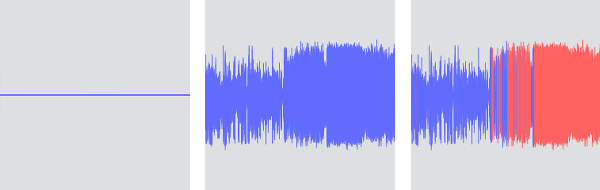
\includegraphics[width=\columnwidth]{figs/conditions-horz.png}
\caption{The three conditions tested. From left to right: no waveform, normal
  waveform and enhanced waveform}
\label{fig:conditions}
\end{figure}

The colour for the colourised waveform was generated by mapping a common speech/music discrimination audio feature to a
colour gradient. The audio feature used to generate the colour was low-energy ratio \citep{Panagiotakis2005}, which is
a mesure of how often the energy of the audio signal drops below a moving threshold. As speech has silences between
words, its energy drops below the threshold more frequently than music.
%It is commonly used as a basis for speech/music discrimination systems. %TODO cite

The threshold can be set as a fixed value \citep{Liang2005}, a function of a moving average \citep{Ericsson2009} or
moving peak value \citep{Saunders1996}.  In the case of this experiment, we configured the threshold as the third
percentile of RMS energy in a one second sliding window. These parameters were set empirically by testing them against
radio programme recordings.

We mapped the low energy ratio to a colour gradient which was blue for low values (representing speech) and to pink
for high values (representing music). We chose the shade of blue to match that used in StarTrack and the pink is
its inverse colour.

%Three different methods were used to visualize the audio: a normal waveform, a colourised waveform and a blank
%display (no waveform). The blank visualization acts as a baseline where participants are operating `blind' with no
%visual assistance.

%The colourised waveform (see Section~\ref{sec:studywaveform}) represents a nominal improvement using a
%simple algorithm designed for the task.

%The expected result is that having a waveform is better than having nothing, and that a colourised waveform performs
%better than a normal waveform.

%We created the colourised waveform by modifying the colour of a standard waveform, based on a very simple speech/music
%discrimination (SMD) feature.

%Low energy ratio (also known as `silent interval frequency' and `energy contour
%dip') is a measure of the number of RMS energy frames that fall below a
%threshold. It exploits the fact that speech has freqent silent gaps between
%words, wheras music does not.

%Low energy ratio is a popular, simple and effective scalar metric for
%speech/music discrimination. It works on the principle that speech has intermittent silences (between words) whereas
%music does not. We calculated it by extracting the RMS energy (20ms frames, no overlap) and counting the proportion of
%frames which fall below a threshold.


\subsection{Hypotheses}

The experiment presented in this paper is designed to test the effectiveness of combining speech-recognizer-generated
transcripts in conjunction with pitch-normalized time- compressed speech. In particular, the following hypotheses are
examined:

\newcommand{\subscript}[2]{$#1 _ #2$}
\begin{enumerate}[label=H\arabic*.]
    \item Visualisation affects the number of seek actions used to complete the task, in decreasing order of C1, C2 and C3.
    \item Visualisation affects the time taken to complete the task, in decreasing order of C1, C2 and C3.
    \item Visualisation affects the error of the result, in decreasing order of C1, C2 and C3.
    \item Visualisation affects the reported task load, in decreasing order of C1, C2 and C3.
\end{enumerate}

%{\singlespacing
%\begin{enumerate}
  %\item Waveforms will allow participants to perform speech/music segmentation
  %\begin{enumerate}
    %\item faster
    %\item with less effort
  %\end{enumerate}
  %\item Adding colour to waveforms will allow participants to perform speech/music segmentation
  %\begin{enumerate}
    %\item faster
    %\item with less effort
  %\end{enumerate}
  %\item For speech/music segmentation, participants will rate
  %\begin{enumerate}
   %\item coloured waveforms as easiest to use and least frustrating
   %\item no waveform as hardest to use and most frustrating
  %\end{enumerate}
%\end{enumerate}
%}

We tested these hypotheses using a task-based within-subjects online study. The task was to find and select the music
within a clip of a radio programme. Three different audio visualisations were tested -- no waveform, a normal waveform
and a colourised waveform. The colourised waveform was generated by mapping a common speech/music discrimination
feature to a colour gradient.

We measured how quickly and accurately participants completed the task, and how many actions they took to get there. We
also used questionnaires to collect qualitative information on task load and preference.
We recruited users with experience of using professional audio editing software.

%Recruiting a large number of radio producers to take part in the study would be difficult as it is a small community
%that are not used to participating in scientific trials. For this reason we chose to recruit participants that have
%experience with using professional audio editing software. We ran the trial online to reach as many people as possible.

%Three conditions were tested -- no waveform, a normal waveform and a colourised waveform.
%Each condition was presented three times, for a 
%Low-energy ratio was used to colourise the waveform, as it is well understood speech/music discriminator.
%Audio from real radio programmes was used

% Conditions
%Colour generated by very simple speech/music discriminaton metric
%Metric does not return perfect results, so user must interpret them
%Three conditions - no waveform, waveform and coloured waveform
%Real radio programmes, 5 min clips x 9
%Within-subjects
%Counterbalanced

% Metrics
%We measured speed using the overall time taken to complete the task. To measure effort, we used a combination of user
%actions required to complete the task, and short questionnairre.

% Test data

\subsection{Procedure}

Before the experiment started, we asked the participant about
their gender, age and the following questions, which attempted to gauge their level of
experience.

{\singlespacing
\begin{itemize}
  \item Do you understand what an audio waveform is? [Yes/No]
  \item Have you previously used any consumer audio editing software? (e.g.
    Audacity, GarageBand) [Yes/No]
  \item Have you previously used any professional audio editing software? (e.g.
    ProTools, Logic, Cubase/Nuendo, SADiE, Startrack) [Yes/No]
  \item How many years (if any) have you worked with audio in a professional
    capacity? [\textit{number}]
\end{itemize}
}

The experiment was divided into four stages:

\paragraph{Stage 1: Training}
They were then taken through a training stage where a series of
pop-up boxes explained how to use the interface and they were assisted in making their first submission.

In order to attract a sufficient number of participants while collecting enough data, we designed the experiment so it
could be completed in 10--15 mins. This led to to repeat each condition three times, for a total of nine tasks.
Each of the conditions were presented in groups to avoid potential confusion caused by jumping between conditions, and
to allow a questionnaire to be presented after each condition.

\paragraph{Stage 2: Task}

In order to make it possible for the experiment to completed in 10-15 mins, we used a sequence of nine tasks.

\paragraph{Stage 3: Task load questionairre}

After completing the tasks for a given condition, we asked participants to rate the workload of each task using the
NASA Task Load Index (NASA-TLX) metric \citep{Hart1988}.  With NASA-TLX, subjects rate the task using six subscales,
then make pairwise comparisons on the perceived importance of the subscales. The importance weightings are used to
combine the subscales into an overall rating for the task. For our experiment, we chose to exclude the second part of
the measurement to collect what is commonly called `Raw TLX' \citep{Hart2006}. We did this to reduce the time required
for data collection, and to allow us to analyse each subscale individually.

The TLX subscales are listed below:

{\singlespacing
\begin{itemize}
  \item Mental Demand -- How mentally demanding was the task? [very low/very high]
  \item Physical Demand -- How physically demanding was the task? [very low/very high]
  \item Temporal Demand -- How hurried or rushed was the pace of the task?  [very low/very high]
  \item Performance -- How successful were you in accomplishing what you were asked to do? [perfect/failure]
  \item Effort -- How hard did you have to work to accomplish your level of performance? [very low/very high]
  \item Frustration -- How insecure, discouraged, irritated, stressed, and annoyed were you? [very low/very high]
\end{itemize}
}

\paragraph{Stage 4: Comparison}
At the end of the experiment, participants were asked to compare the conditions directly by selecting which they
thought were the easiest and most frustrating. A thumbnail image representing each visualisation was shown to remind
the participants of how they looked.

\subsection{Metrics}
We configured the interface to log and timestamp every action the user made, including each seek, play/pause, select
and zoom action. We also used these metrics to calculate the task completion time, defined as the time between the
first user action and the last select action.

%\paragraph{Other}
%In addition to the above measures, we recorded the browser and operating system each participant used, and the date
%and time at which they submitted each data point.

\subsection{Test data}
We used radio programme clips for the audio data, by choosing a representative selection of programme formats, musical
genres and radio stations.  We sourced the audio content from BBC recordings of transmission (ROT) and selected
five-minute clips that contained only one section that could be categorised as music.  The clips are described in
Table~\ref{tab:clips}.


\begin{table}[htbp]
  \begin{center}
    {\small
    \begin{tabular}{|l|l|l|l|l|l|}
      \hline
      \multicolumn{1}{|l|}{\textbf{Clip}} & \textbf{Network} & \textbf{Title} 
      & \textbf{Prog format} & \textbf{Music genre} \\ \hline
      Training & Radio 4 & Desert Island Discs & Interview & Ambient \\ \hline
      1 & 1 Xtra & Sian Anderson & Breakfast & Dance \\ \hline
      2 & 6 Music & Lauren Laverne & Single & Indie \\ \hline
      3 & Radio 2 & Ken Bruce & Phone quiz & Lounge \\ \hline
      4 & Radio 3 & Breakfast show & Single & Classical \\ \hline
      5 & 5 Live & Sports report & Sports & Band \\ \hline
      6 & Radio 1 & Zane Lowe & Interview & Rap \\ \hline
      7 & Radio 2 & Jo Whiley & Review & Pop \\ \hline
      8 & Radio 4 & Afternoon drama & Drama & Classical \\ \hline
      9 & Radio 4 & Front Row & Interview & Alternative \\ \hline
    \end{tabular}
    }
  \end{center}
  \caption{Descriptions of the radio programmes used for the evaluation}
  \label{tab:clips}
\end{table}

We used latin squares were used to generate the test sequences so that each audio clip was only used once per
participant, and to ensure balanced conditions with no carryover effects.


\subsection{Sequence}\label{sec:studysequence}

We chose to group the presentation of the conditions rather than interleave them (e.g. AAABBBCCC instead of ACACBABCB).
We did this to be able to capture task load feedback directly after each condition, and to avoid confusions caused
by switching too often.
After all tasks we completed, we asked the participant the comparions questions.

Each audio clip can only be used once per participant, otherwise they would be able to remember where the music was.
To generate the sequence of nine audio clips, we used a Williams design Latin square, which we generated using the
`crossdes' package\footnote{\url{http://cran.r-project.org/web/packages/crossdes/index.html}} in R.  We used Latin
squares to block out variation from participants and the order of presentation, and used the Williams design as it is
balanced for first-order carryover effects. As the sequence length is odd, the Williams design uses two latin squares
to produce an $18\times9$ matrix.

To generate the visualisation sequence, we needed to produce a balanced $18\times3$ matrix. We did this by taking three
columns from our $18\times9$ and mapping the values $1-3$, $4-6$ and $7-9$ to 1, 2 and 3, respectively.  By testing
each column of the $18\times9$ matrix, we found that the middle three columns produced a balanced sequence with and
minimised the carryover effects.

%\begin{table}
%\centering
  %{\small
    %\begin{tabular}{|rrrrrrrrr|}
      %\hline
      %1 & 2 & 9 & 3 & 8 & 4 & 7 & 5 & 6 \\ 
      %3 & 3 & 3 & 2 & 2 & 2 & 1 & 1 & 1 \\ 
      %\hline
      %2 & 3 & 1 & 4 & 9 & 5 & 8 & 6 & 7 \\ 
      %1 & 1 & 1 & 3 & 3 & 3 & 2 & 2 & 2 \\ 
      %\hline
      %3 & 4 & 2 & 5 & 1 & 6 & 9 & 7 & 8 \\ 
      %2 & 2 & 2 & 1 & 1 & 1 & 3 & 3 & 3 \\ 
      %\hline
      %4 & 5 & 3 & 6 & 2 & 7 & 1 & 8 & 9 \\ 
      %3 & 3 & 3 & 2 & 2 & 2 & 1 & 1 & 1 \\ 
      %\hline
      %5 & 6 & 4 & 7 & 3 & 8 & 2 & 9 & 1 \\ 
      %1 & 1 & 1 & 3 & 3 & 3 & 2 & 2 & 2 \\ 
      %\hline
      %6 & 7 & 5 & 8 & 4 & 9 & 3 & 1 & 2 \\ 
      %2 & 2 & 2 & 1 & 1 & 1 & 3 & 3 & 3 \\ 
      %\hline
      %7 & 8 & 6 & 9 & 5 & 1 & 4 & 2 & 3 \\ 
      %3 & 3 & 3 & 2 & 2 & 2 & 1 & 1 & 1 \\ 
      %\hline
      %8 & 9 & 7 & 1 & 6 & 2 & 5 & 3 & 4 \\ 
      %1 & 1 & 1 & 3 & 3 & 3 & 2 & 2 & 2 \\ 
      %\hline
      %9 & 1 & 8 & 2 & 7 & 3 & 6 & 4 & 5 \\ 
      %2 & 2 & 2 & 1 & 1 & 1 & 3 & 3 & 3 \\ 
      %\hline
      %6 & 5 & 7 & 4 & 8 & 3 & 9 & 2 & 1 \\ 
      %1 & 1 & 1 & 2 & 2 & 2 & 3 & 3 & 3 \\ 
      %\hline
      %7 & 6 & 8 & 5 & 9 & 4 & 1 & 3 & 2 \\ 
      %2 & 2 & 2 & 3 & 3 & 3 & 1 & 1 & 1 \\ 
      %\hline
      %8 & 7 & 9 & 6 & 1 & 5 & 2 & 4 & 3 \\ 
      %3 & 3 & 3 & 1 & 1 & 1 & 2 & 2 & 2 \\ 
      %\hline
      %9 & 8 & 1 & 7 & 2 & 6 & 3 & 5 & 4 \\ 
      %1 & 1 & 1 & 2 & 2 & 2 & 3 & 3 & 3 \\ 
      %\hline
      %1 & 9 & 2 & 8 & 3 & 7 & 4 & 6 & 5 \\ 
      %2 & 2 & 2 & 3 & 3 & 3 & 1 & 1 & 1 \\ 
      %\hline
      %2 & 1 & 3 & 9 & 4 & 8 & 5 & 7 & 6 \\ 
      %3 & 3 & 3 & 1 & 1 & 1 & 2 & 2 & 2 \\ 
      %\hline
      %3 & 2 & 4 & 1 & 5 & 9 & 6 & 8 & 7 \\ 
      %1 & 1 & 1 & 2 & 2 & 2 & 3 & 3 & 3 \\ 
      %\hline
      %4 & 3 & 5 & 2 & 6 & 1 & 7 & 9 & 8 \\ 
      %2 & 2 & 2 & 3 & 3 & 3 & 1 & 1 & 1 \\ 
      %\hline
      %5 & 4 & 6 & 3 & 7 & 2 & 8 & 1 & 9 \\ 
      %3 & 3 & 3 & 1 & 1 & 1 & 2 & 2 & 2 \\ 
      %\hline
    %\end{tabular}
    %}
    %\caption{Sequence of presentation of audio clips (top) and visualisations (bottom).}
    %\label{tab:clipseq}
%\end{table}

\subsection{Analysis}
We wanted to ensure that all participants completed their tasks correctly.  To do so, we rejected any participant that
submitted a segment with an error of more than five seconds. We calculated the error as the sum of the absolute error
of the in-point and out-point.

%\begin{figure}[ht]
  %\begin{center}
    %$ |t_{in}-t_{inREF}| + |t_{out}-t_{outREF}| \leq 5 $\\[1em]
    %where $t_{in}$ and $t_{out}$ are the in- and out-points of each selection, in seconds,
    %and $t_{inREF}$ and $t_{outREF}$ are the ground truth in- and out-points of the music.
  %\end{center}
  %\caption{Acceptance criteria for the experiment}
  %\label{eq:accept}
%\end{figure}

For the TLX metrics, we used repeated measures ANOVA to test for statistically significant differences in the task load
responses. We then used Tukey's honest significant difference (HSD) post-hoc test to make pairwise comparisons between
the visualisation for each metric.

For the usage data, we couldn't re-use the audio clips, so the participants only experienced a subset of all
combinations of visualisations and audio clips. This resulted in missing data, which prevented using from using
repeated measures ANOVA. Instead, we used a linear mixed model as it can tolerate missing values and account for the
fact that multiple responses from the same person are more similar than responses from other people.

We used SPSS to perform a linear mixed effects analysis of the relationship between visualisation and seek actions. As
fixed effects, we entered visualisation into the model. As random effects, we had intercepts for subjects and audio
clips. Visual inspection of residual plots did not reveal any obvious deviations from homoscedasticity or normality.
P-values were obtained by likelihood ratio tests of the full model with the effect in question against the model
without the effect in question.

%\paragraph{Box plot}
%A box plot \citep{McGill1978} is a technique used to graph distributions by their quartile values (i.e. 25th, 50th and
%75th percentiles). An example can be seen in Figure~\ref{fig:seekbox}. The box extends from the first to the third
%quartile, with the second quartile (median) marked as a line through the box.  Lines are drawn from the box to the
%minimum and maximum, known as `whiskers', however data determined to be outliers are marked separately as crosses.  The
%95\% confidence interval of the median is marked as a notch in the box.

%\paragraph{ANOVA}
%Analysis of variance is a method of testing whether the mean values of several groups are equal or not. It assumes that
%the observations are independent, that the data have a normal distribution, and that the variance within the groups are
%similar. One-way ANOVA tests for a null hypothesis that the means values of the factors are the same.

%\paragraph{Tukey's test}
%If the null hypothesis is rejected using ANOVA, we know that there is a difference between the factors, but we don't
%know which ones. Tukey's test is a post-hoc analysis for discovering the difference between individual factors.  It
%assumes that the observations are independent and that the variance within the groups are similar.

%When Tukey's test is graphed, the mean values are represented by a dot with a line either side showing the confidence
%interval. Confidence intervals which don't overlap can be said to be significantly different.

%\paragraph{Standardisation}
%Some observations can be biased through participant behaviour. For example, person A navigates audio recordings by
%quickly clicking along the timeline while person B navigates with only a few considered clicks. To block this factor,
%the responses of each participant can be standardised so that they have a mean value of 0 and a standard deviation of
%1. This allows the difference between different participants responses to be measured fairly.

%Standardisation maps observations to the `\textbf{standard score}'. This is a dimensionless unit which represents the
%number of standard deviations an observation is above the mean.

\subsection{System description}

To conduct the experiment, we developed a web-based test interface, shown in Figure~\ref{fig:visualisation-interface}.
The interface enabled the user to listen to and navigate the audio, then mark and submit a selection. It also provided
training and captured responses to questionnaires.  A detailed technical explanation of the interface can be found in
Section~\ref{sec:browser-audio-interface}.

The interface displayed the overall visualisation as well as a zoomed in view. The user could play/pause the audio and
control the zoom level, and mark in-- and out-points using buttons. The user could also use either of the
visualisations to navigate the audio, by clicking on it, or adjust their segment by dragging on the edge.  Training was
conducted using a `pop-up tour', which guided the user through the interface's operation using a series of pop-up text
boxes for each feature.

\begin{figure}[ht]
\centering
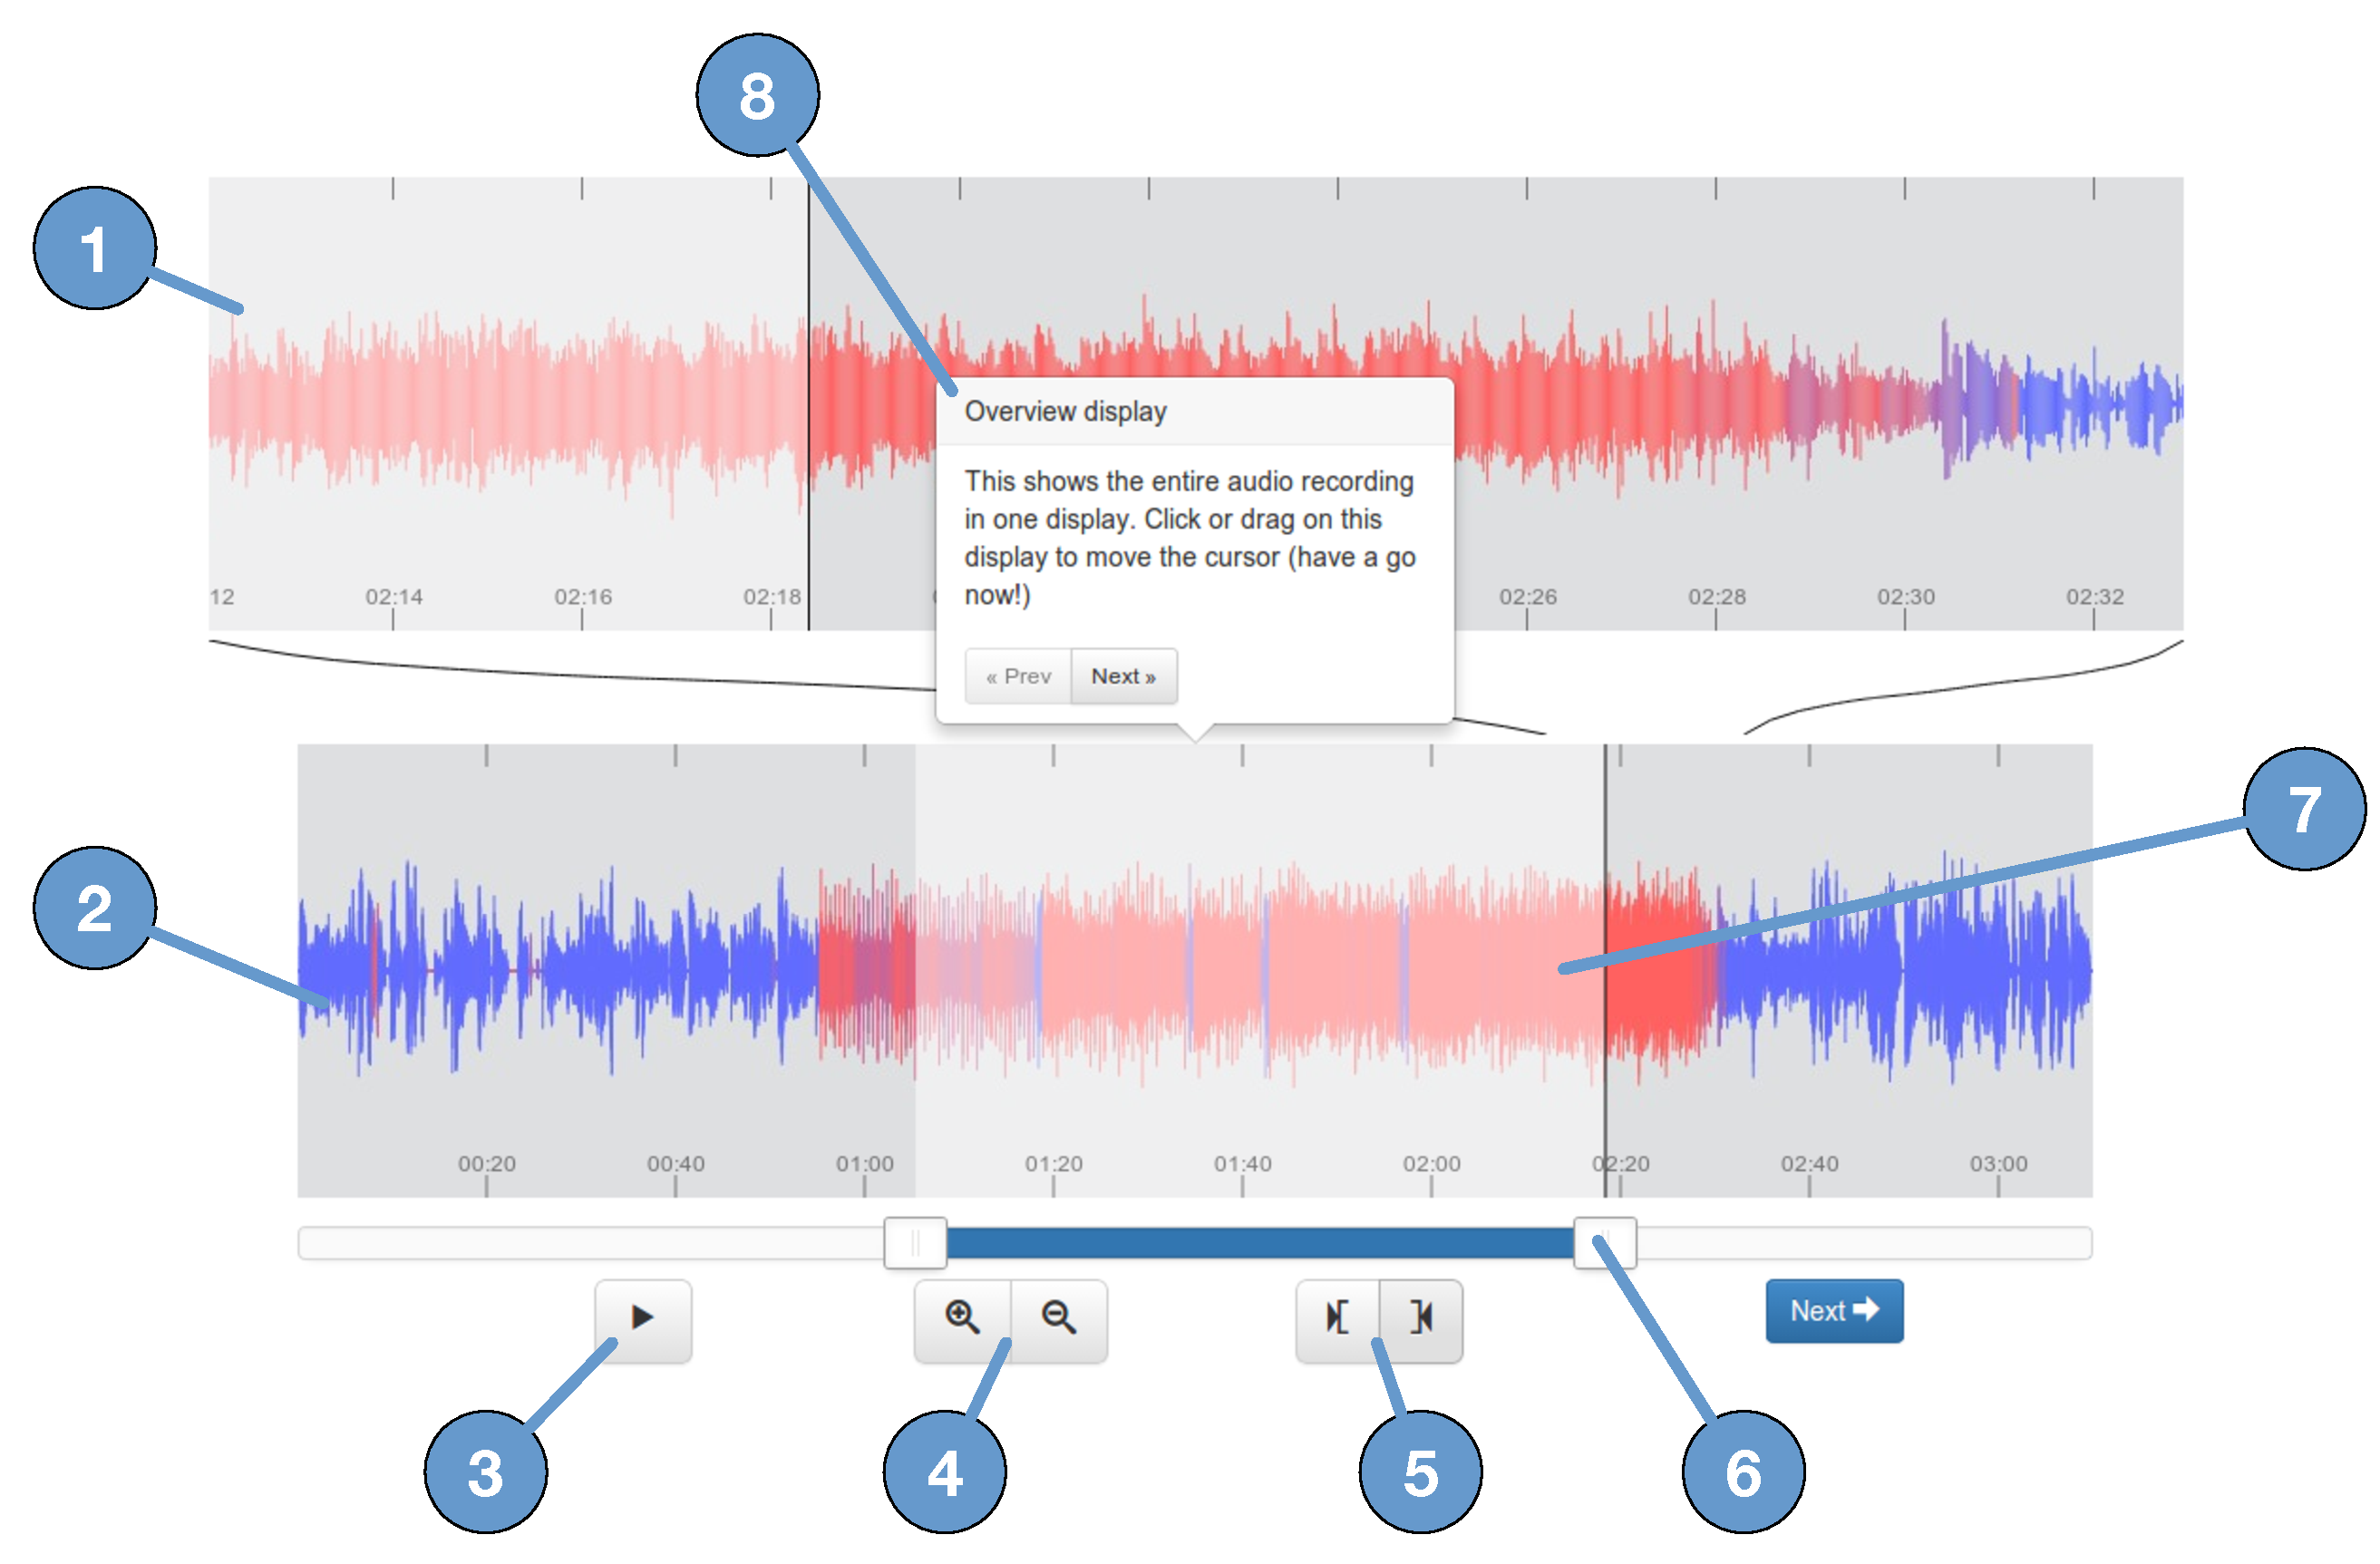
\includegraphics[width=\columnwidth]{figs/browser-audio-interface.pdf}
\caption{Screenshot of the test interface with the following features:
zoomed-in audio visualisation (1),
overview audio visualisation (2),
play/pause control (3),
zoom in/out control (4),
mark in/out buttons (5),
selection slider (6),
selection highlighting (7),
and training pop-ups (8).}
\label{fig:visualisation-interface}
\end{figure}

We generated the visualisations from the audio clips using a plugin framework we developed called `Vampeyer', which
maps the results of an audio analysis algorithm to a bitmap image. We then integrated those images into our test
interface using in an interactive web-based audio visualisation library we developed called `BeatMap'.  We have written
in more detail about Vampeyer and BeatMap in Sections \ref{sec:vampeyer} and \ref{sec:beatmap}, respectively. We have
also released both systems as open source software.

\section{Results}
63 responses were completed in the three weeks the experiment ran. Emails linking to the experiment were sent to
roughly 450 people, which gives a conversion rate of 14\%. This was much higher than expected. Informal feedback
suggested that many people enjoyed participating due to the listening and task-based nature of the experiment. 

Of the 63 experiments completed, only 41 passed the acceptance criteria (see Section~\ref{sec:study1-acceptance}
meaning that 35\% of participants were rejected. Figure~\ref{fig:rejectdaw} shows that none of the rejected
participants had experience of using a professional audio editor, suggesting that the mistakes may have been made due
to inexperience with audio interfaces.

\begin{figure}[ht]
  \centering
  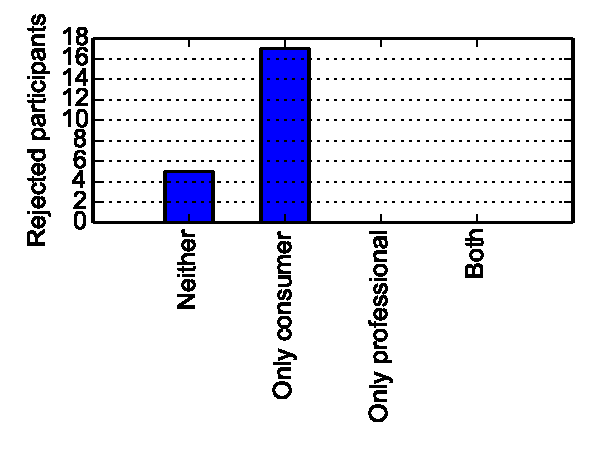
\includegraphics[width=0.5\textwidth]{figs/reject-daw.pdf}
  \caption{Response of rejected participants when asked whether they had previously used consumer/professional audio
    editing software}
  \label{fig:rejectdaw}
\end{figure}

Figure~\ref{fig:rejectvis} plots the number of incorrect responses received for each visualisation, which shows that no
particular visualisation is responsible for the mistakes. However, Figure~\ref{fig:rejectclip} shows that there is
variation in the mistakes made for each clip, particularly clips 4 and 5. An analysis of the incorrect in and out
points for these clips found that the mistakes were varied and don't suggest a systematic problem. 

\begin{figure}[ht]
\centering
\begin{subfigure}{.5\textwidth}
  \centering
  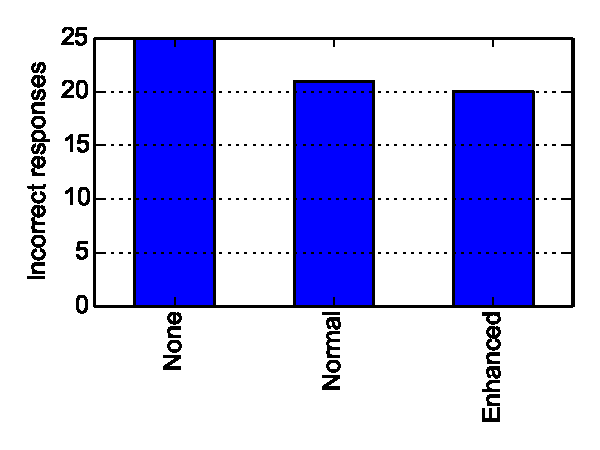
\includegraphics[width=\linewidth]{figs/rejects-vis.pdf}
  \caption{By visualisation}
  \label{fig:rejectvis}
\end{subfigure}%
\begin{subfigure}{.5\textwidth}
  \centering
  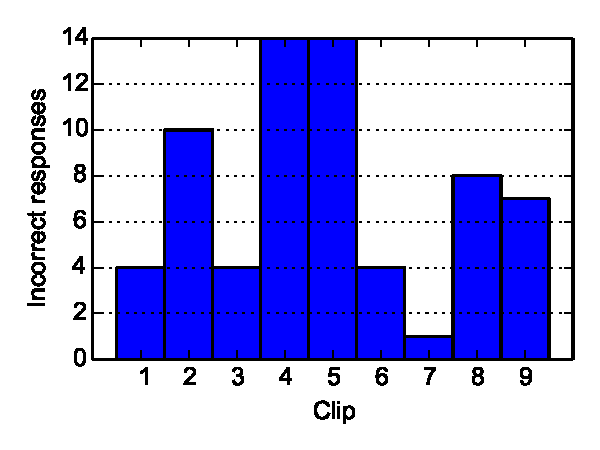
\includegraphics[width=\linewidth]{figs/rejects-clip.pdf}
  \caption{By clip}
  \label{fig:rejectclip}
\end{subfigure}
\caption{Analysis of incorrect responses}
\label{fig:rejects}
\end{figure}

\subsection{Demographics}
The demographic of the participants showed a heavy bias (80\%) of male participants, and a larger proportion in the
26-45 age range (see Figure~\ref{fig:age}). This reflects the population to which the experiment was promoted (see
Section~\ref{sec:promo}) and is not expected to skew the results.

\begin{figure}[ht]
  \centering
  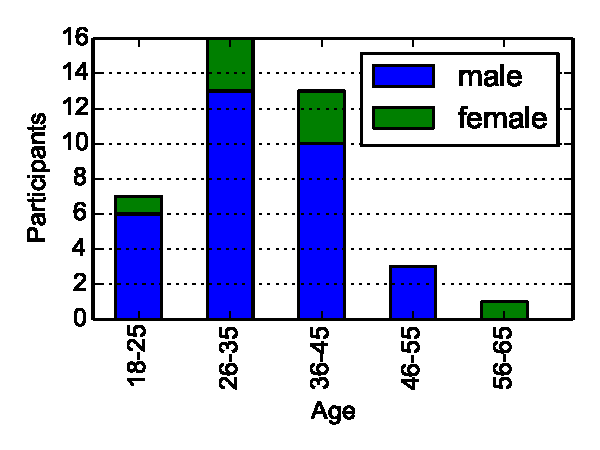
\includegraphics[width=0.5\textwidth]{figs/age.pdf}
  \caption{Age and gender of participants. Male/female ratio was 32/8
    (80\%/20\%). One participant declined to respond to the question.}
  \label{fig:age}
\end{figure}

Most participants had previous experience of using both consumer and professional audio editing software (see
Figure~\ref{fig:experiencedaw}), with 29\% of participants only having experience of consumer software or no experience
at all.

When asked about years of professional audio experience, 39\% of participants reported having no experience, with the
remainder being spread out up to a maximum of 25 years (see Figure~\ref{fig:experienceyears}). Interestingly, the
answer people gave peaks at the 5 and 10--year marks, where people may have given a rounded number rather than an
accurate figure.

\begin{figure}[ht]
\centering
\begin{subfigure}{.5\textwidth}
  \centering
  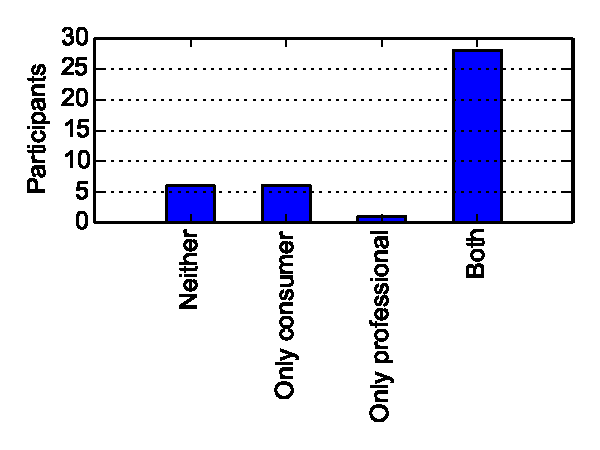
\includegraphics[width=\textwidth]{figs/daw.pdf}
  \caption{Previous use of audio editing software}
  \label{fig:experiencedaw}
\end{subfigure}%
\begin{subfigure}{.5\textwidth}
  \centering
  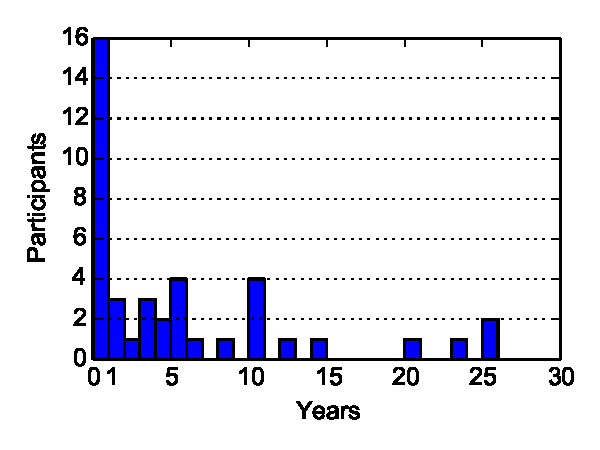
\includegraphics[width=\linewidth]{figs/experience.pdf}
  \caption{Years of professional audio experience}
  \label{fig:experienceyears}
\end{subfigure}
\caption{Response of participants to questions about experience}
\label{fig:experience}
\end{figure}


\subsection{Performance metrics}\label{sec:studymetrics}
An analysis was carried out on the performance metrics that were measured while participants used the interface (see
Section~\ref{sec:metrics}).

\begin{figure}
  \centering
  \begin{subfigure}[t]{0.5\textwidth}
    \centering
    \begin{tikzpicture} 
    \begin{axis}[
      width=\textwidth,
      ylabel=Seek actions (count),
      xtick={1,2,3},
      xticklabels={Audio,Waveform,Coloured}]
      \addplot[black,mark=*]
        plot[error bars/.cd, y dir=both, y explicit]
        coordinates {
          (1, 29.5) +- (3.7,3.7)
          (2, 24.3) +- (3.6,3.6)
          (3, 16.8) +- (3.1,3.1)
        };
    \end{axis} 
    \end{tikzpicture}
    \caption{Seek actions}
  \end{subfigure}%
  ~
  \begin{subfigure}[t]{0.5\textwidth}
    \centering
    \begin{tikzpicture} 
    \begin{axis}[
      width=\textwidth,
      ylabel=Error (seconds),
      xtick={1,2,3},
      xticklabels={Audio,Waveform,Coloured}]
      \addplot[black,mark=*]
        plot[error bars/.cd, y dir=both, y explicit]
        coordinates {
          (1, 0.645) +- (0.121,0.121)
          (2, 0.610) +- (0.121,0.121)
          (3, 0.523) +- (0.109,0.109)
        };
    \end{axis} 
    \end{tikzpicture}
    \caption{Error}
  \end{subfigure}

  \begin{subfigure}[t]{0.5\textwidth}
    \centering
    \begin{tikzpicture} 
    \begin{axis}[
      width=\textwidth,
      ylabel=Time (seconds),
      xtick={1,2,3},
      xticklabels={Audio,Waveform,Coloured}]
      \addplot[black,mark=*]
        plot[error bars/.cd, y dir=both, y explicit]
        coordinates {
          (1, 70.6) +- (16.76,16.76)
          (2, 68.7) +- (16.49,16.49)
          (3, 59.7) +- (16.47,16.47)
        };
    \end{axis} 
    \end{tikzpicture}
    \caption{Time}
  \end{subfigure}
  \caption{Mean metric values with 95\% confidence intervals}
\end{figure}

\paragraph{Seek action}
The number of seek actions made was standardised for each participant. This was done to reduce variation due to
different search styles (i.e. frequent aimless seeking along the timeline vs. infrequent purposeful seeking)

ANOVA found there to be a difference between the visualizations for $p < 0.01$ and Tukey's HSD test (see
Figure~\ref{fig:seektukey}) showed that the number of seek actions are different for each visualization in favour of
the colourised version, again for $p < 0.01$. Even without standardisation, the same result holds for $p < 0.05$.

%\begin{figure}[ht]
%\centering
%\begin{subfigure}{.5\textwidth}
  %\centering
  %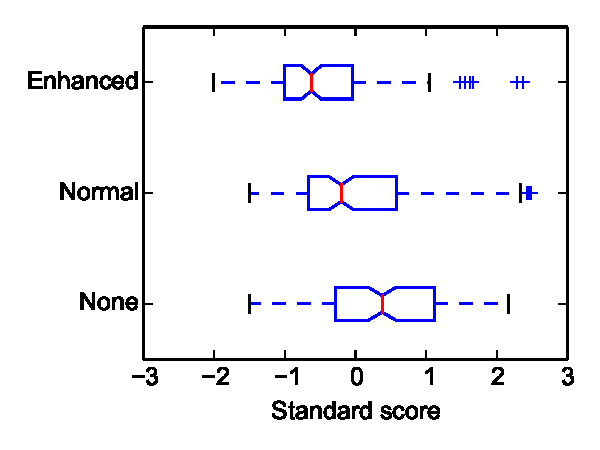
\includegraphics[width=\textwidth]{figs/seek-std.pdf}
  %\caption{Box plot}
  %\label{fig:seekbox}
%\end{subfigure}%
%\begin{subfigure}{.5\textwidth}
  %\centering
  %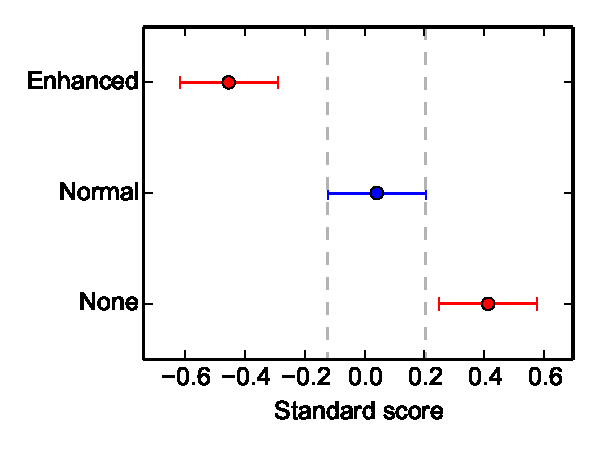
\includegraphics[width=\linewidth]{figs/seek-std-tukey99.pdf}
  %\caption{Tukey's test (99\% confidence interval)}
  %\label{fig:seektukey}
%\end{subfigure}
%\caption{Number of seek actions, standardised per participant}
%\label{fig:seek}
%\end{figure}

\paragraph{Selection time}
The time taken to make a selection was calculated as the difference between the time the play button was first pressed
and the time the final selection was made. This reduces variation due to participants not starting the task immediately
and participants who made a selection, then checked the rest of the recording for other pieces of music. The mean and
standard deviation of the selection time was standardised for each participant to reduce the effect of people's natural
pace.

%\begin{figure}[ht]
%\centering
%\begin{subfigure}{.5\textwidth}
  %\centering
  %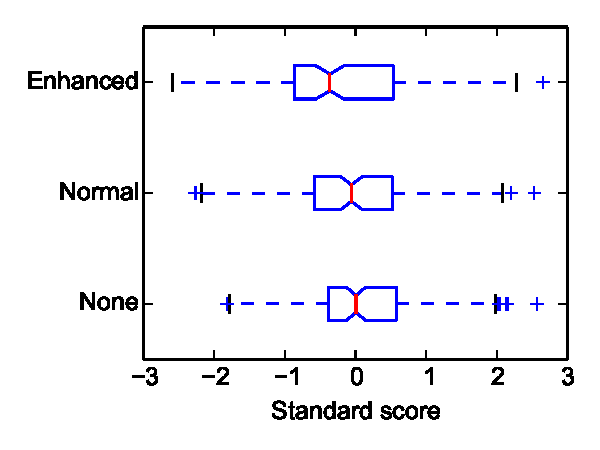
\includegraphics[width=\textwidth]{figs/playstart-to-selectend-std.pdf}
  %\caption{Box plot}
  %\label{fig:selecttimebox}
%\end{subfigure}%
%\begin{subfigure}{.5\textwidth}
  %\centering
  %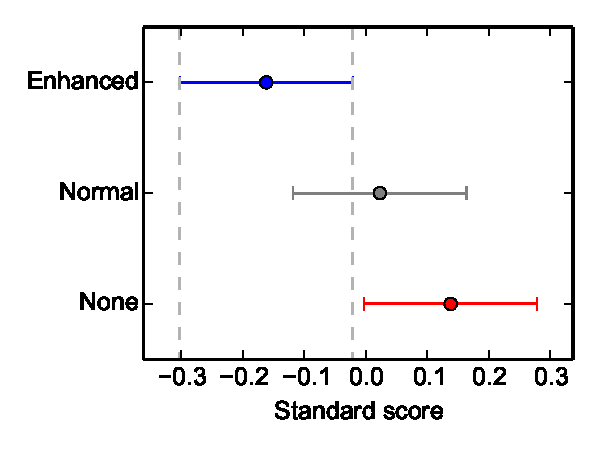
\includegraphics[width=\linewidth]{figs/playstart-to-selectend-std-tukey95.pdf}
  %\caption{Tukey's test (95\% confidence interval)}
  %\label{fig:selecttimetukey}
%\end{subfigure}
%\caption{Selection time (time between start of playback and final selection), standardised per participant}
%\label{fig:selecttime}
%\end{figure}

ANOVA showed that there was a significant difference between visualizations for $p < 0.05$. Tukey's test (see
Figure~\ref{fig:selecttimetukey}) found that there was a difference between no visualization and the colourised version,
but not between either of them and the normal waveform.

\paragraph{Error}
The absolute error of the selections made by each participant were calculated for the inpoint, outpoint and sum of
both. ANOVA found there to be no difference between the visualisations for the inpoint or the sum, but found a
significant difference ($p < 0.05$) for the outpoint.  Tukey's test (see Figure~\ref{fig:outpointerrtukey}) found that
the absolute error of the outpoint for the colourised visualization was significantly lower than the other two
visualizations, but that the other two were no different.

This is an unexpected result which is difficult to explain, as the inpoint and sum errors were not even close to
rejecting the null hypothesis ($p > 0.3$).  Although the result is significant, the improvement in accuracy is only
about 150ms which is small in the context of 5-minute recordings.

%\begin{figure}[ht]
%\centering
%\begin{subfigure}{.5\textwidth}
  %\centering
  %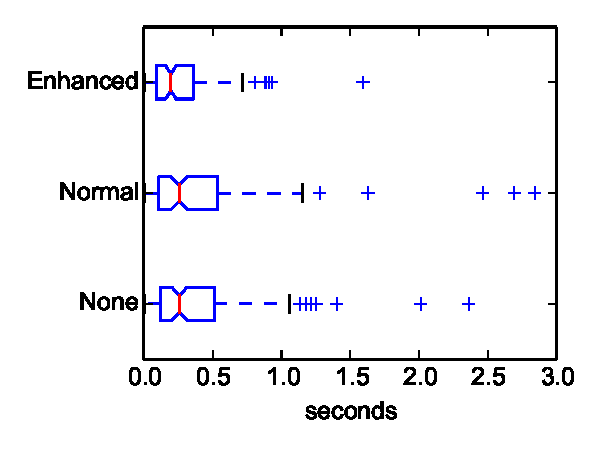
\includegraphics[width=\textwidth]{figs/outpoint-abserr.pdf}
  %\caption{Box plot}
  %\label{fig:outpointerrbox}
%\end{subfigure}%
%\begin{subfigure}{.5\textwidth}
  %\centering
  %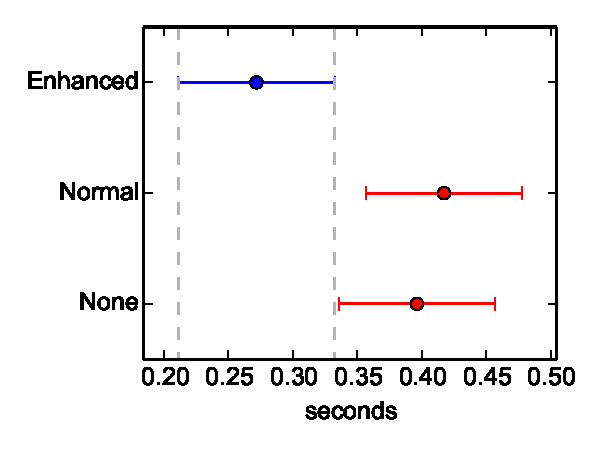
\includegraphics[width=\linewidth]{figs/outpoint-abserr-tukey95.pdf}
  %\caption{Tukey's test (95\% confidence interval)}
  %\label{fig:outpointerrtukey}
%\end{subfigure}
%\caption{Absolute error for the outpoint of selections}
%\label{fig:outpointerr}
%\end{figure}

%\paragraph{Zoom}
%The experimental interface included two displays -- one overview display covering the length of the recording, and a
%zoomed display which showed a magnified part of that. The number of times the zoom in and zoom out buttons were pressed
%was logged. The sum of these values for each visualization is shown in Figure~\ref{fig:zoomtotal}. By subtracting zoom
%out from zoom in, we can infer what the final zoom level was when the response was submitted. The final zoom levels for
%each visualization are shown in Figure~\ref{fig:zoomfinal}.

%\begin{figure}[h!]
%\centering
%\begin{subfigure}{.5\textwidth}
  %\centering
  %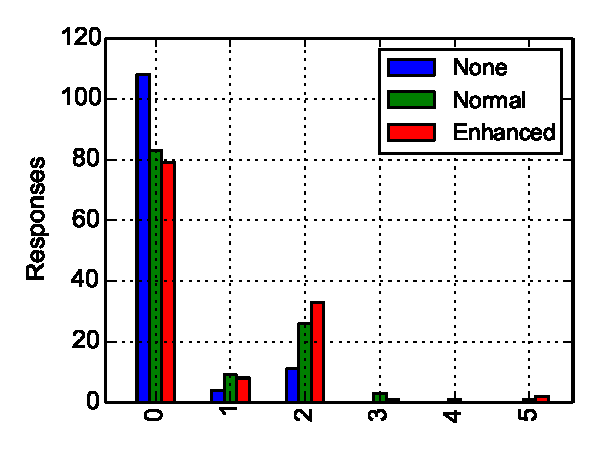
\includegraphics[width=\linewidth]{figs/zoomtotal.pdf}
  %\caption{Total zoom actions}
  %\label{fig:zoomtotal}
%\end{subfigure}%
%\begin{subfigure}{.5\textwidth}
  %\centering
  %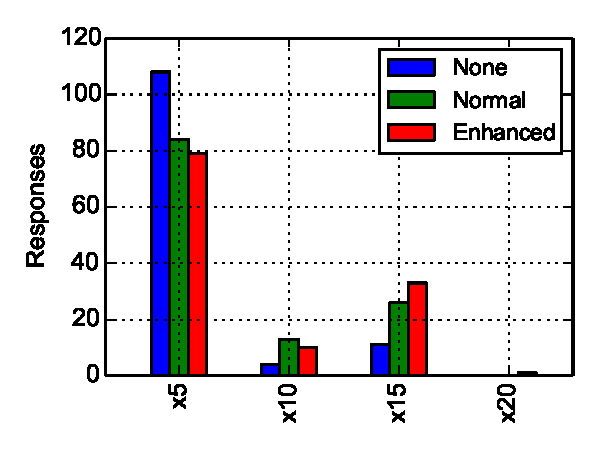
\includegraphics[width=\linewidth]{figs/zoomfinal.pdf}
  %\caption{Final zoom level}
  %\label{fig:zoomfinal}
%\end{subfigure}
%\caption{Analysis of zoom usage}
%\label{fig:zoom}
%\end{figure}

%Most of the time, participants didn't touch the zoom controls and opted to leave it on the default x5 zoom level, which
%displays roughly one minute of audio across 1045 pixels ($\sim$50ms per pixel). Other than the x5 level, x15 was more
%popular than x10 for all visualizations and x20 was barely used at all.

\subsection{Comparison}
Participants were asked to directly compare the three visualizations at the end of the experiment. The results are
shown in Figure~\ref{fig:compare}.

\begin{figure}[ht]
\centering
\begin{subfigure}{.5\textwidth}
  \centering
  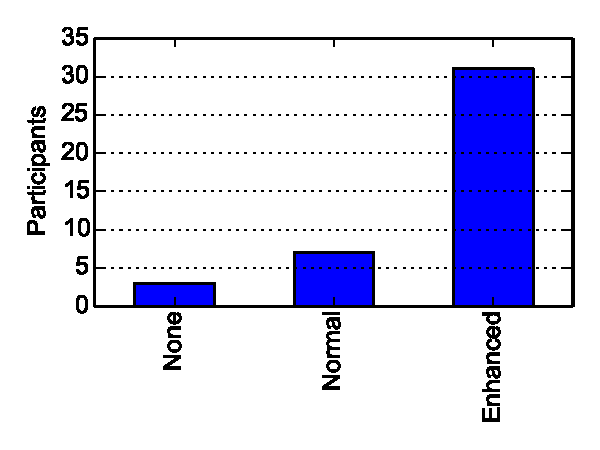
\includegraphics[width=\textwidth]{figs/easiest.pdf}
  \caption{Easiest to use}
  \label{fig:easiest}
\end{subfigure}%
\begin{subfigure}{.5\textwidth}
  \centering
  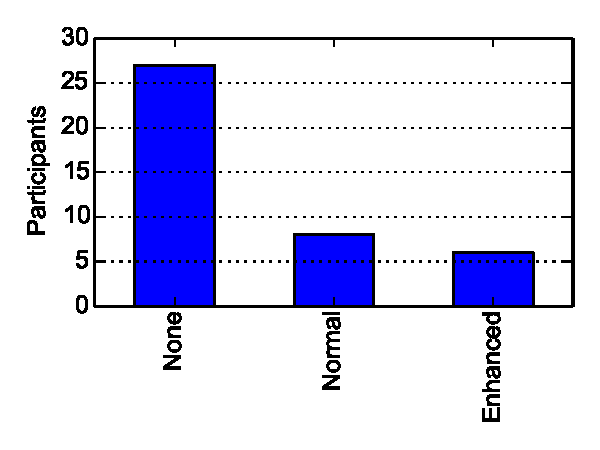
\includegraphics[width=\linewidth]{figs/frustrating.pdf}
  \caption{Most frustrating}
  \label{fig:frustrating}
\end{subfigure}
\caption{Response of participants when asked to compare the visualisations
  using different criteria}
\label{fig:compare}
\end{figure}

76\% of participants thought that the colourised waveform was the easiest to use, with the normal waveform receiving
17\% of votes and 7\% for no waveform.  The strong preference for the colourised waveform over the others shows that
participants thought the additional information added using colour made their task easier.

Having no waveform was considered by two-thirds of participants to be the most frustrating condition, followed by the
normal waveform at 20\% and colourised waveform at 15\%. Although this is another strong result in favour of using
waveforms, the results are not quite as strong as the ones on ease of use. It is possible that the false positives and
negatives present in the colourised waveform caused some people to select it as the most frustrating.

\subsection{Task load index}
The TLX responses were standardised to account for variation in the way different people assign scores. The
distributions of the standardised scores for each visualization are shown in Figure~\ref{fig:tlx}.

\begin{figure}
  \centering
  \begin{subfigure}[t]{0.5\textwidth}
    \centering
    \begin{tikzpicture} 
    \begin{axis}[
      width=\textwidth,
      ylabel=Effort,
      xtick={1,2,3},
      xticklabels={Audio,Waveform,Coloured}]
      \addplot[black,mark=*]
        plot[error bars/.cd, y dir=both, y explicit]
        coordinates {
          (1, -0.122) +- (1.49,1.49)
          (2, -2.244) +- (1.51,1.51)
          (3, -4.220) +- (1.28,1.28)
        };
    \end{axis} 
    \end{tikzpicture}
    \caption{Effort}
  \end{subfigure}%
  ~
  \begin{subfigure}[t]{0.5\textwidth}
    \centering
    \begin{tikzpicture} 
    \begin{axis}[
      width=\textwidth,
      ylabel=Frustration,
      xtick={1,2,3},
      xticklabels={Audio,Waveform,Coloured}]
      \addplot[black,mark=*]
        plot[error bars/.cd, y dir=both, y explicit]
        coordinates {
          (1, -0.829) +- (2.03,2.03)
          (2, -2.976) +- (1.67,1.67)
          (3, -5.268) +- (1.24,1.24)
        };
    \end{axis} 
    \end{tikzpicture}
    \caption{Frustration}
  \end{subfigure}%

  \begin{subfigure}[t]{0.5\textwidth}
    \centering
    \begin{tikzpicture} 
    \begin{axis}[
      width=\textwidth,
      ylabel=Mental demand,
      xtick={1,2,3},
      xticklabels={Audio,Waveform,Coloured}]
      \addplot[black,mark=*]
        plot[error bars/.cd, y dir=both, y explicit]
        coordinates {
          (1, -1.390) +- (1.68,1.68)
          (2, -2.585) +- (1.45,1.45)
          (3, -4.585) +- (1.23,1.23)
        };
    \end{axis} 
    \end{tikzpicture}
    \caption{Mental demand}
  \end{subfigure}%
  ~
  \begin{subfigure}[t]{0.5\textwidth}
    \centering
    \begin{tikzpicture} 
    \begin{axis}[
      width=\textwidth,
      ylabel=Performance,
      xtick={1,2,3},
      xticklabels={Audio,Waveform,Coloured}]
      \addplot[black,mark=*]
        plot[error bars/.cd, y dir=both, y explicit]
        coordinates {
          (1, -5.415) +- (1.10,1.10)
          (2, -6.317) +- (1.11,1.11)
          (3, -7.341) +- (0.88,0.88)
        };
    \end{axis} 
    \end{tikzpicture}
    \caption{Performance}
  \end{subfigure}%

  \begin{subfigure}[t]{0.5\textwidth}
    \centering
    \begin{tikzpicture} 
    \begin{axis}[
      width=\textwidth,
      ylabel=Physical demand,
      xtick={1,2,3},
      xticklabels={Audio,Waveform,Coloured}]
      \addplot[black,mark=*]
        plot[error bars/.cd, y dir=both, y explicit]
        coordinates {
          (1, -3.122) +- (1.81,1.81)
          (2, -4.098) +- (1.45,1.45)
          (3, -6.171) +- (1.08,1.08)
        };
    \end{axis} 
    \end{tikzpicture}
    \caption{Physical demand}
  \end{subfigure}%
  ~
  \begin{subfigure}[t]{0.5\textwidth}
    \centering
    \begin{tikzpicture} 
    \begin{axis}[
      width=\textwidth,
      ylabel=Temporal demand,
      xtick={1,2,3},
      xticklabels={Audio,Waveform,Coloured}]
      \addplot[black,mark=*]
        plot[error bars/.cd, y dir=both, y explicit]
        coordinates {
          (1, -3.171) +- (1.75,1.75)
          (2, -3.268) +- (1.51,1.51)
          (3, -4.878) +- (1.39,1.39)
        };
    \end{axis} 
    \end{tikzpicture}
    \caption{Temporal demand}
  \end{subfigure}%
  \caption{Mean TLX values with 95\% confidence intervals}
\end{figure}

\definecolor{lightred}{RGB}{255,204,204}
\definecolor{lightamber}{RGB}{255,204,153}
\definecolor{lightgreen}{RGB}{204,255,204}
\newcommand{\highsig}{\cellcolor{lightgreen}}
\newcommand{\medsig}{\cellcolor{lightamber}}
\newcommand{\nosig}{\cellcolor{lightred}}
\begin{table}
\resizebox{\textwidth}{!}{
\begin{tabular}{ | l | l | l | l | }
\hline
  & Audio vs Waveform & Audio vs Coloured & Waveform vs Coloured \\ \hline
	Seek actions & \highsig$<0.01$ & \highsig$<0.01$ & \highsig$<0.01$ \\ \hline
	Error & \nosig$>0.05$ & \highsig$<0.01$ & \medsig$<0.05$ \\ \hline
	Time & \nosig$>0.05$ & \highsig$<0.01$ & \highsig$<0.01$ \\ \hline
	TLX Effort & \medsig$<0.05$ & \highsig$<0.01$ & \highsig$<0.01$ \\ \hline
	TLX Frustration & \medsig$<0.05$ & \highsig$<0.01$ & \medsig$<0.05$ \\ \hline
	TLX Mental & \nosig$>0.05$ & \highsig$<0.01$ & \highsig$<0.01$ \\ \hline
	TLX Performance & \nosig$>0.05$ & \highsig$<0.01$ & \medsig$<0.05$ \\ \hline
	TLX Physical & \nosig$>0.05$ & \highsig$<0.01$ & \highsig$<0.01$ \\ \hline
  TLX Temporal & \nosig$>0.05$ & \nosig$>0.05$ & \medsig$<0.05$ \\ \hline
\end{tabular}}
\caption{$p$-values of pairwise comparisons}
\end{table}

%\begin{figure}[p]
  %\centering
  %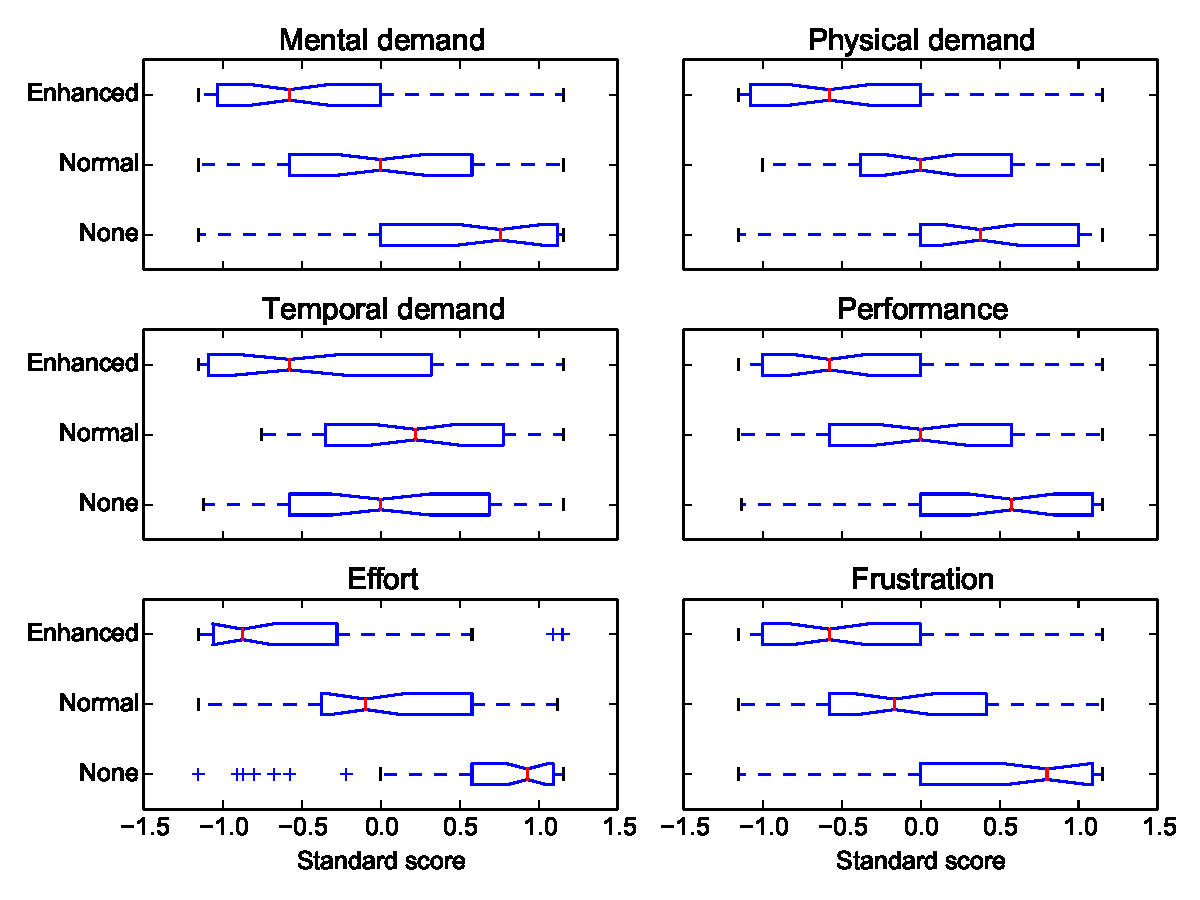
\includegraphics[width=\textwidth]{figs/tlx-std.pdf}
  %\caption{Standard score of NASA Task Load Index responses for each visualization, standardised per participant.}
  %\label{fig:tlx}
%\end{figure}

%\begin{figure}[p]
  %\centering
  %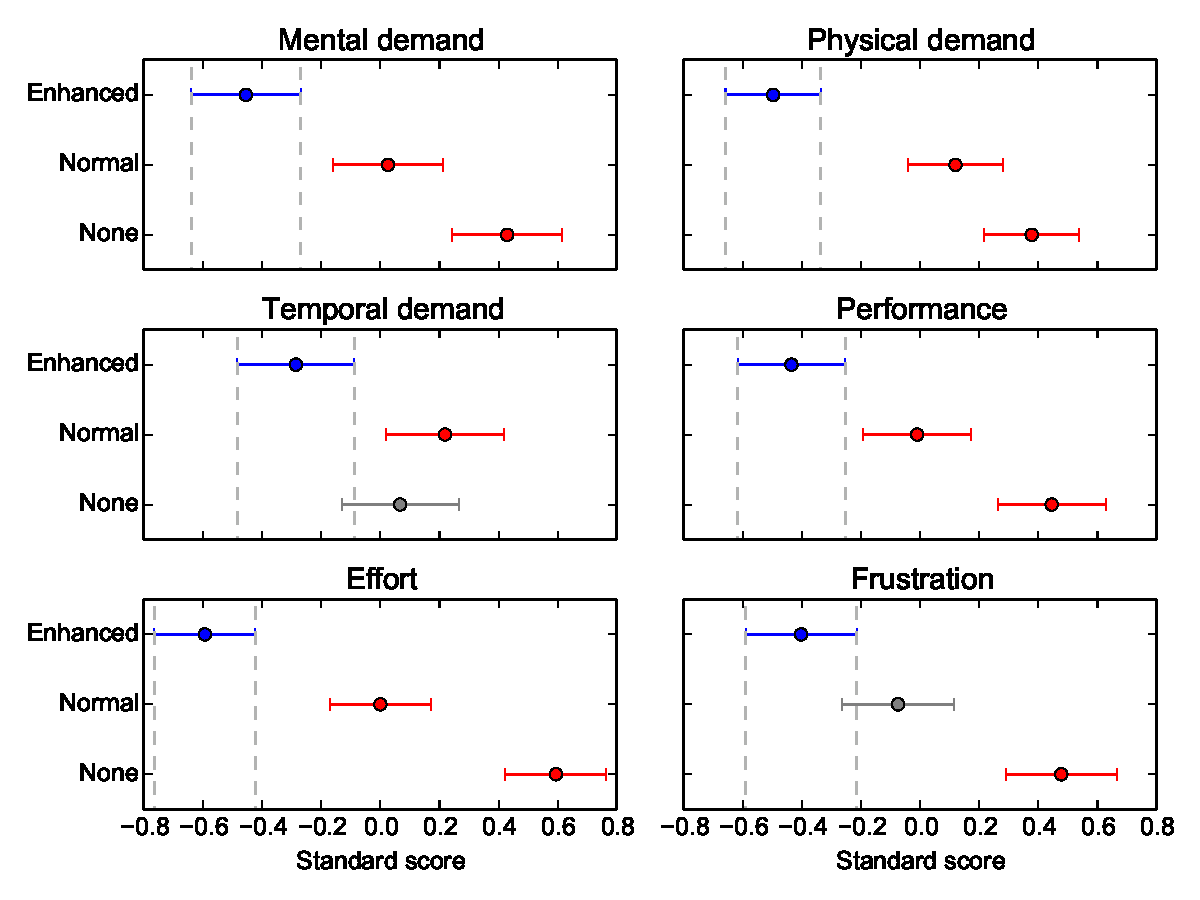
\includegraphics[width=\textwidth]{figs/tlx-std-tukey95.pdf}
  %\caption{Standard score of NASA Task Load Index responses for each visualization, standardised per participant.}
  %\label{fig:tlxtukey}
%\end{figure}

ANOVA found there to be significant differences between the visualizations in all TLX metrics for $p < 0.01$. Tukey's
test (see Figure~\ref{fig:tlxtukey}) found that for $p < 0.05$, the colourised waveform outperformed no waveform in all
metrics except temporal demand, and outperformed the normal waveform in all metrics except frustration. The normal
waveform outperformed no waveform in mental demand, performance, effort and frustration.

Some scepticism should be given to the physical and temporal demand metrics, as it's not entirely clear what is meant
by that terminology in the context of the task. Participants are not working against the clock, not are they doing
anything other than moving the mouse. Although some participants may consider fewer clicks of the mouse to represent
reduced physical demand, we cannot assume that others thought the same.

\subsection{Interaction behaviour}
This section looks at how participants used the features available in the online audio interface, full described in
Section~\ref{sec:iface}.
%Informal observation of some participants as they completed the experiment
%revealed that some people used the interface in different ways. For example,
%when one participant had completed their selection, they scanned through the
%remaining unselected content to check that there were no other pieces of music.

%\begin{figure}[ht]
%\centering
%\begin{subfigure}{.5\textwidth}
  %\centering
  %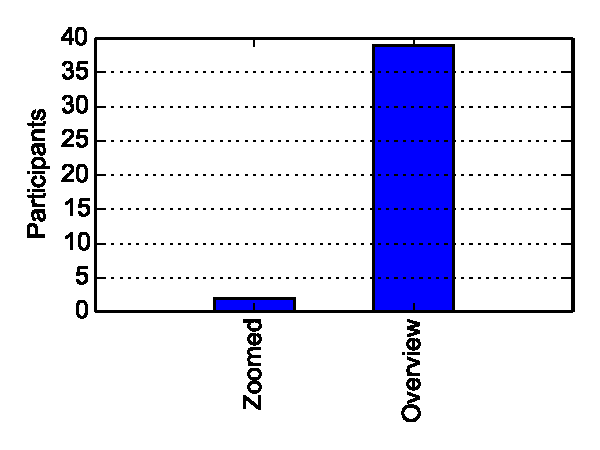
\includegraphics[width=\linewidth]{figs/top-v-bot-pref.pdf}
  %\caption{Display}
  %\label{fig:displaypref}
%\end{subfigure}%
%\begin{subfigure}{.5\textwidth}
  %\centering
  %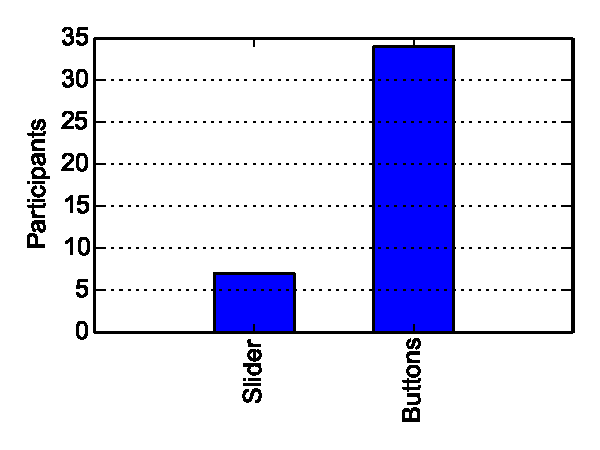
\includegraphics[width=\linewidth]{figs/mark-v-slide-pref.pdf}
  %\caption{Selection method}
  %\label{fig:selectpref}
%\end{subfigure}
%\caption{Preference of participants}
%\label{fig:pref}
%\end{figure}

%\paragraph{Top/bottom display}
%There are two displays that make up the interface -- a zoomed display at the top and an overview display on the bottom.
%Either of the displays can be used to navigate the recording and make selections.

%For each participant, the number of tasks where they used the zoom display more than the overview (and vice-versa) were
%counted. Figure~\ref{fig:displaypref} shows number of participants who, on average, used the zoomed or overview display
%more.

%The results show a clear preference for using the overview display more than the zoom display. Coupled with the results
%of zoom usage in Section~\ref{sec:studymetrics}, we can see that for this task most people opted just to work in the
%overview display, despite only having a resolution of roughly 300ms per pixel.

%An analysis of the overview and zoom display's usage between different visualization methods did not find any notable
%difference.

%\paragraph{Selection method}
%The design of the interface gave participants two methods of making a selection -- buttons to mark in and out points
%using the cursor, and a slider where the in and out points could be dragged around. The cursor can be moved around in
%both the overview and zoomed displays, whereas the slider is only available at the x1 zoom level. This makes the
%buttons more useful for fine edits, where high precision is needed. When using the slider, the selection display
%updates as you move it making it easier for people to see where their selection is.

%For each response, the method with the most actions was found and these preferences were summed for each participant to
%calculate their overall preference. The results are shown in Figure~\ref{fig:selectpref}.

%The buttons were the most popular method of making a selection, with only 17\% of people using the slider more.
%Informal feedback found that some people has a strong preference for using the slider but were frustrated that there
%wasn't a second slider available on the zoomed display.

%\section{Results}
%63 responses were received in the three weeks the experiment ran. 35\% of participants were rejected, which was higher
%than expected. An analysis of the rejected participants found that none had experience of using professional audio
%editing software, which suggests that the errors could be due to lack of experience with audio interfaces.

%The demographic of accepted participants reflected the population which was recruited: 80\% male with a larger
%proportion in the 26-45 age range. This imbalance is not expected to affect the result. Two-thirds of accepted
%participants had experience of using professional audio editing software, with the remaining participants having
%consumer-level experience or less. 39\% reported having no professional experience with audio.

%Figure~\ref{fig:seekpdf} shows the distribution of the number of seek actions for each visualization. On average, the
%number of seek actions required to select the music is lowest for the enhanced waveform and highest for no waveform.
%However, individual participants had different styles of interaction; for example, some people had a tendency to seek
%around a lot whereas others didn't. In order to account for this, the performance and TLX metrics were standardised for
%each participant.

%\begin{figure}[!h]
%\centering
%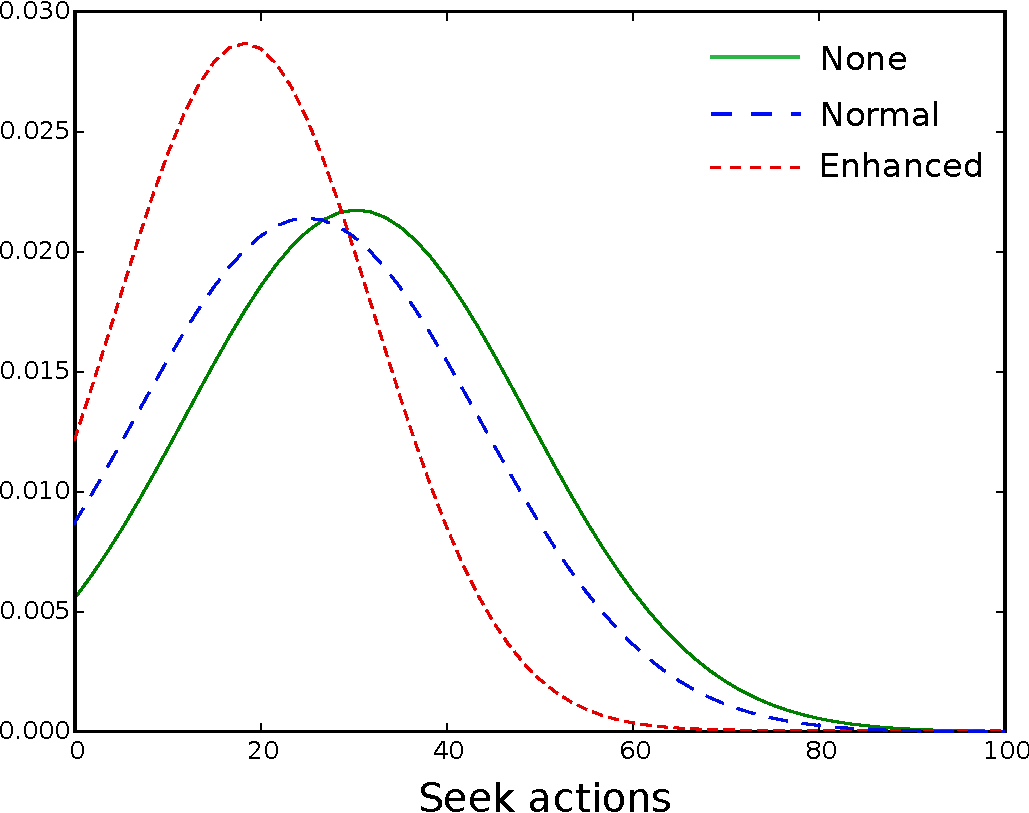
\includegraphics[width=0.6\columnwidth]{figs/seek-pdf.pdf}
%\caption{Probability density function of number of seek actions for each
%visualization}
%\label{fig:seekpdf}
%\end{figure}

%For each metric, the standardisation function (see Equation~\ref{eq:standard}) subtracts the mean of the participant's
%scores and divides by the standard deviation. This maps observations to the `standard score', which is a dimensionless
%unit that represents the number of standard deviations an observation is above the mean.

%\begin{equation}
%std(x) = \frac{x - \mu_{part}}{\highsigma_{part}}
%\label{eq:standard}
%\end{equation}

%The performance and TLX metrics of the 41 accepted participants were analysed using ANOVA.  Significant results were
%found for the number of seek actions ($F_{2,40}=30, p<0.001$) and the selection time ($F_{2,40}=3.2,p\medsig$<0.05$$).  Tukey's
%test shows that the enhanced waveform required fewer seek actions than the normal waveform, and the normal waveform
%required fewer than no waveform (see Figure~\ref{fig:tukeyseekselect}). The selection time was shorter for the enhanced
%waveform compared to no waveform, but the normal waveform was not significantly different.

%\begin{figure}[!h]
%\centering
%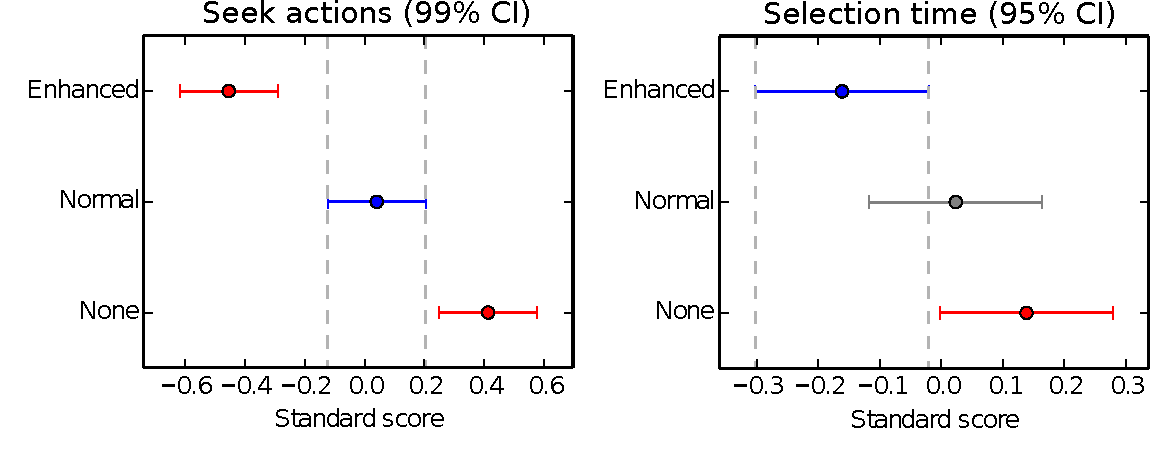
\includegraphics[width=\columnwidth]{figs/seek-select.pdf}
%\caption{Tukey's test for mean number of seek actions and mean selection time}
%\label{fig:tukeyseekselect}
%\end{figure}

%Significant results were found for each of the NASA-TLX metrics ($F_{2,40}>4.8,p\highsig$<0.01$$). The normal waveform performed
%better than no waveform for mental demand, performance, effort and frustration (see Figure~\ref{fig:tlx}). The enhanced
%waveform performed better than the normal waveform for mental, physical and temporal demand, performance and effort.

%\begin{figure}[!h]
%\centering
%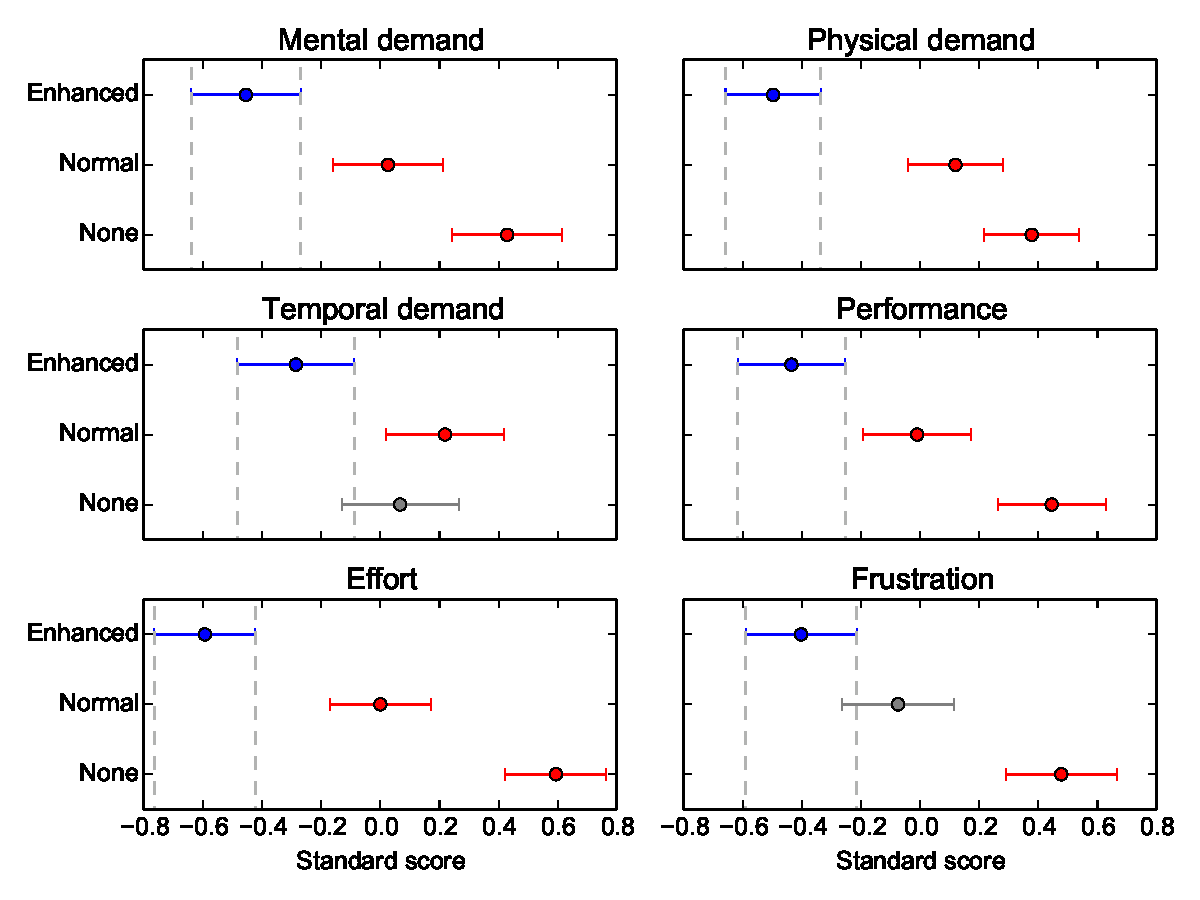
\includegraphics[width=\columnwidth]{figs/tlx-std-tukey95.pdf}
%\caption{Tukey's test for mean of NASA-TLX metrics (95\% CI). Lower is
  %better.}
%\label{fig:tlx}
%\end{figure}

%76\% of participants thought that the enhanced waveform was the easiest to use with the normal waveform scoring 17\%.
%Two-thirds thought that having no waveform was the most frustrating condition with 20\% choosing the normal waveform.

\section{Discussion}

\section{Conclusion}
The normal waveform required fewer seek actions than nothing but was not significantly faster. It scored better than
nothing for mental demand, performance and frustration.

The enhanced waveform required fewer seek actions than the normal waveform and was significantly faster than nothing.
It performed better than the normal waveform for mental demand, performance and effort.

%This experiment used a browser-based audio interface to conduct a within-subjects online study of how users performed
%in finding and selecting music with different audio waveforms. Three conditions were tested -- no waveform, a normal
%waveform and a waveform that was colourised using a simple speech/music discriminator.

%Compared to no waveform, the normal waveform required fewer seek actions and was rated better in terms of mental
%demand, performance, effort and frustration. Finding and selecting music with the colourised version took less time
%than with no waveform. Compared to the normal waveform, it required fewer seek actions and was rated better in terms of
%mental, physical and temporal demand, performance and effort.

%\subsection{Further work}
%The results indicate that the waveform can be significantly improved, even with a simple enhancement. The next stages
%of this research will focus on development of audio analysis and visualization algorithms/tools that address the needs
%of people working in radio production. This will be followed by an analysis of the real-world benefit of using these
%new tools.


\cleardoublepage
% !TeX root = main.tex
\chapter{Audio editing workflows in radio production}\label{chp:ethno}

% link to previous chapter

We saw in Chapter~\ref{chp:colourised} that we can improve the performance of at least one audio editing task by
enhancing the audio visualization. We were interested in exploring how we could apply these techniques to radio
production, to help producers create programmes more efficiently.  To continue this research, we needed to decide which
production tasks we should target. This required an understanding of the tasks involved in radio production, and of the
challenges producers face in their roles.

% radio production is not well documented and hard to access

%Radio production is conducted globally on a large scale. The BBC alone has 9 national and 40 local radio stations,
%%and BBC World Service, which broadcasts in 29 languages. 
%each of which broadcast 24/7.

There are two classic books that document the radio production process. \citet{McLeish2015}, now in its sixth edition,
provides a broad overview of the practice of radio production with an emphasis on editorial, organisational and
business concerns.  \citet{Hausman2012}, currently in its ninth edition, covers the more practical aspects of radio
production including the use and operation of tools and equipment.  Despite the valuable contribution of these
publications, they present a high-level overview of production practice that does not fully address the real-life
challenges and issues that radio producers face in the industry.

It can be difficult for those working outside of the radio industry to learn about the challenges of radio production.
We could only find one published study that involved radio producers, by \citet{Dunaway2000}, which was based on his
experience of being a documentary producer. This lack of studies may be a result of the limited number of radio
producers, and their demanding workload, which can make it challenging to recruit them for research.  For example,
\citet{Kim2003} worked with National Public Radio (NPR) to develop a system for searching speech archives.  Despite
working directly with NPR, they were unsuccessful in recruiting radio producers to evaluate their system as there were
not many producers, and they did not volunteer because they were too busy.

% hard for researchers to develop solutions without understanding challenges and problems
% lots of technology could help, but how to choose which?

There are many semantic audio and user interface technologies that have the potential to improve the radio production
workflow. Speech/music discrimination \citep{Wieser2014}, speaker diarization \citep{AngueraMiro2012}, speaker
identification \citep{Lee1999a} and automatic speech recognition \citep{Junqua1995} can all be benefitial for use in
radio systems \citep{Raimond2014,Bell2015}. However, it is difficult to know how best to apply these techniques without
a solid understanding of the radio production process.

Without a good understanding of how radio production works in reality, and the challenges that producers face in their
work, it can be difficult for researchers outside of the industry to contribute developments that might benefit radio
producers.

Previous studies of professional broadcast environments have focused on how producers collaborate during live
production \citep{Engstroem2010,Perry2009}, by using video recordings to analyse the interactions between producers.
The scope of this study was much wider and covered the production of programmes over a number of weeks. As such, an
ethnographic approach was taken so that all aspects of the production could be considered.

Experiments into the use of higher-level representations like text are starting to appear, such as the video editors
from Loviscach \citep{Loviscach2011a} and Hyperaudio \citep{Boas2011}.

However, without a detailed understanding of the production workflows, it can be difficult to know which of these
technologies have the most potential, or how they can be integrated into the workflow.

% what we did in this chapter
To help us better understand the radio production process, we conducted three ethnographic case studies of practice in
BBC Radio.
In Section~\ref{sec:ethno-method} we outline the design of our study.
Section~\ref{sec:ethno-results} presents the results of each case studies,
Section~\ref{sec:ethno-discussion} discusses the findings and
Section~\ref{sec:ethno-conclusion} presents the conclusion.

\section{Methodology}\label{sec:ethno-method}

% objective of study

The objective of our study was to document the radio production workflow, so we could identify opportunities for making
improvements through the application of semantic audio technology.

% focus on audio editing
Most radio content is broadcast live. In these cases, the content is produced in real-time, so there is no opportunity
to produce the programme any faster. However, many types of programmes, such as documentaries and drama, are
pre-produced using audio editing software. Here, the production process is many times longer than the programme, so
there are opportunities to make the production process more efficient.

\subsection{Data collection}
% ethnography, direct observation
We used ethnographic research methods to study the culture of radio production in BBC Radio. We chose to use direct
observation to collect our data, where we witnessed production first-hand without taking part.  We did this so that we
could observe the real-world process, as opposed to a theoretical one, and take into account the context of the working
environment. Additionally, producers are very busy and direct observation allowed us to collect the data without adding
to the producer's workload, while being as unobtrusive as possible.

We recorded the data by writing field notes during observation. We were not able to use video or audio recording as
much of the observation took place in open-plan offices that deal with sensitive information. We also used any time
between activities to ask the participants clarifying questions.

% sampling
Due to the scale and variety of the radio operations at the BBC, it would be impossible to cover all production genres
and techniques. To limit the scope of our work, we followed a ``maximum variation sampling'' strategy \citep[p.
172]{Patton1990} to choose a small number of heterogeneous case studies. We aimed to select programmes that varied in
genre, as we speculated that these would have different cultures and work practices.

The time needed to produce programmes can vary significantly, with some being produced over many weeks or months. To
reduce our observation time, we worked with the producer of each programme to create a schedule of observations that
sampled every stage of the process. This allowed us to capture the entire workflow without having to be present
throughout.

% recruitment
\subsection{Recruitment}
We recruited participants using an invitation email sent to BBC R\&D's contact list of studio managers working in BBC
Radio. This process put us in touch with three producers who were interested in participating. The producers worked on
the programmes and in the departments listed below:
\begin{itemize}
	\item Hourly news bulletin (Radio Summaries, BBC News)
	\item ``15 Minute Drama'' radio drama (London Radio Drama, BBC Radio)
	\item ``The Report'' documentary (Radio Current Affairs, BBC News)
\end{itemize}

These three programmes (news report, drama, documentary) fulfilled our criteria for a heterogeneous sample of
programmes from different genres.

% data collection
\subsection{Procedure}
We used direct observation to collect the data for our study with a single researcher. The researcher observed the
production of each programme from the beginning of audio recording/collection, to the point where the audio had been
finalised. The observation did not focus on a single member of the team, instead covering the entire team that
contributed to the audio production. This allowed us to study the different roles and how they interact.  The
production teams were observed in their normal place of work. This allowed us to take into account the context of the
environment in which the teams work, both in terms of the physical location and layout, and of the tools and software
they use to perform their tasks.

We worked with the producer of each programme to design a schedule of observation that would cover the entire
production process. Each programme required a different amount of time. Observing the news bulletin took half-a-day,
the drama took two days, and the documentary took four days. 

The researcher typed or hand-wrote field notes throughout the observation and interviews. When the team members were
not busy, the researcher asked clarifying questions to ensure they understood the reasons and motivation behind the
workflow. The notes specifically included the following:

{\singlespacing
\begin{itemize}
	\item \textbf{Roles} -- Who are the teams members? What are their responsibilities? Are any other teams involved?
	\item \textbf{Environment} -- What is the location? How is the physical space laid out?
	\item \textbf{Tools} -- What purpose are the tools used for? How do the users operate the tools?
	\item \textbf{Tasks} -- What tasks are involved? Who does what? What sequence do they take place?
	\item \textbf{Challenges} -- Were there any problems? Which activities were demanding or mundane?
\end{itemize}
}

The researcher also took photographs of any relevant locations, tools or other items, with the permission of the
participant.

\subsection{Analysis}

We started by populating a list of roles involved in the production, graphed the political structure and wrote a
description of each of their responsibilities. We wrote a description of the working environment in which the
production took place, including the location, the tools that were used, and how they were used. We also drew a map of
the physical environment, including the spatial layout of the team members.

We used hierarchical task analysis \citep{Kirwan1992,Annett2000} to deconstruct the production process into a sequence
of individual actions. We assigned each action to the role that was responsible and the location in which it took
place. We then used a partitioned operational sequence diagram \citep{Kirwan1992} to display the sequence of tasks from
top to bottom, arranged into columns to indicate the role and location.

Finally, we identified any challenges that were noted by the researcher, and wrote a description of the current
approach and any suggested improvements that could be made.

\section{Study results}\label{sec:ethno-results}

In this section, we present the results of our three ethnographic case studies. For each study, we describe the roles
and responsibilities of the team members, and the environment and tools that are used. We then detail the results of
the task analysis we performed, and list the challenges we identified.

%The vast majority of radio production work in the BBC uses a networked audio production system called \textit{dira!}
%\citep{SCISYS2015}. It is colloquially known as `VCS', after the former name of the company that makes it. All audio
%content is kept on distributed storage and the system is accessed using various pieces of software: `StarTrack' is a
%multi-track audio editor, `Orion' is an audio recorder and single-track editor and `Highlander' is used to browse
%recordings and metadata. 

\subsection{News bulletin}\label{sec:news}
The Radio Summaries team at BBC News (known as ``summaries'') write news bulletins for most of the national radio
networks. The 6pm and 10pm reports are handled by different teams, as are the bulletins for Radio 1, 1Xtra, Asian
Network and Radio 5.  The bulletins written by the team are read live on-air by a newsreader at the start of every
hour.

The researcher observed the team for five hours during a morning weekday shift, from 7am to midday. The pace of work in
the team was so fast that there was little time to talk to the participants to ask any questions, so the results are
mostly based on direct observation.

\subsubsection{Roles and responsibilities}\label{sec:news-roles}
Summaries is run by an \textit{assistant editor} who leads between two and four \textit{broadcast journalists}. The
team work 24 hours a day on three eight-hour rolling shifts to report breaking news stories and their developments
throughout the day.

The role of each broadcast journalist is to select and write a series of short text summaries of the day's news stories
for a given radio network.  They also enhance the summmaries by finding, editing and inserting audio clips of reports
or interviews.  Each journalist produces one bulletin per hour, each between two and five minutes long, with between
four and six stories per bulletin.  The length of the bulletin and number of stories depend on the network and the time
of day. For example, Radio 4 bulletins are longer than other networks, and midday bulletins are longer than those at
other times. Even if the stories being covered are the same, the bulletins for each network are written separately so
that they are targeted to the audience of that network.  This is done by varying the language, tone, amount of detail
and level of assumed knowledge.

The assistant editor is the team leader, but also performs the same role as the broadcast journalists. They assign
responsibilities for each radio network's bulletins to a broadcast journalist. Throughout the day, they keep track of
the news stories that are happening and decide which of these should be included in the bulletins. Finally, they read
and approve each bulletin written by the team to check that they are appropriately worded, have been fact-checked, and
comply with the BBC's editorial guidelines.  The assistant editor aims to have the bulletins approved about 15 mins
before the hour.  Once approved, the finished bulletins are read out live by a \textit{newsreader} in a radio studio.

Summaries gather audio content by working with the Intake and Newswire teams, and directly with reporters. The
`\textit{Intake}' team set up and record live incoming audio and video feeds from reporters in the field. They use an
intercom to notify summaries of the incoming feeds so that they can listen-in to the live feeds and provide instant
feedback to the reporter. The `\textit{Newswire}' team provide curated clips of both BBC and ``user-generated content''
that has been submitted by the general public. Summaries also work directly with individual \textit{reporters} who they
commission to record clips for the bulletins. These are recorded and edited by the reporters themselves and provided to
the team directly.

\subsubsection{Environment and tools}
The summaries team sit together at a large desk in the BBC newsroom at New Broadcasting House in London.
Figure~\ref{fig:newsroom} shows the newsroom and Figure~\ref{fig:newsroom-layout} shows the location of the team within
the space. The BBC newsroom houses teams from around the BBC News division and is spatially arranged to facilitate the
fast flow of communication. The teams for each platform (e.g. TV, radio, online) sit on together on desks that fan out
from a central area where the editors sit together. Decisions on which stories to cover are made in this central area,
and are communicated outwards.

Figure~\ref{fig:news-desktop} shows an example of the desks used by members of the radio summaries team. The desk
includes an intercom that can be used to communicate with other teams by using labelled ``push-to-talk'' buttons. A
desktop TV monitor is used to keep an eye on the ``BBC News 24'' TV channel, to track which stories they are currently
reporting. Most communication is within the team, which is helped by sitting close together on a single desk.

\begin{figure}[p]
  \centering
  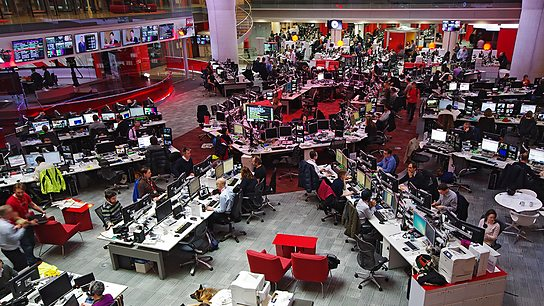
\includegraphics[width=\columnwidth]{figs/newsroom.jpg}
  \caption{The newsroom in BBC New Broadcasting House.}
  \label{fig:newsroom}
\end{figure}

\begin{figure}[p]
	\centering
	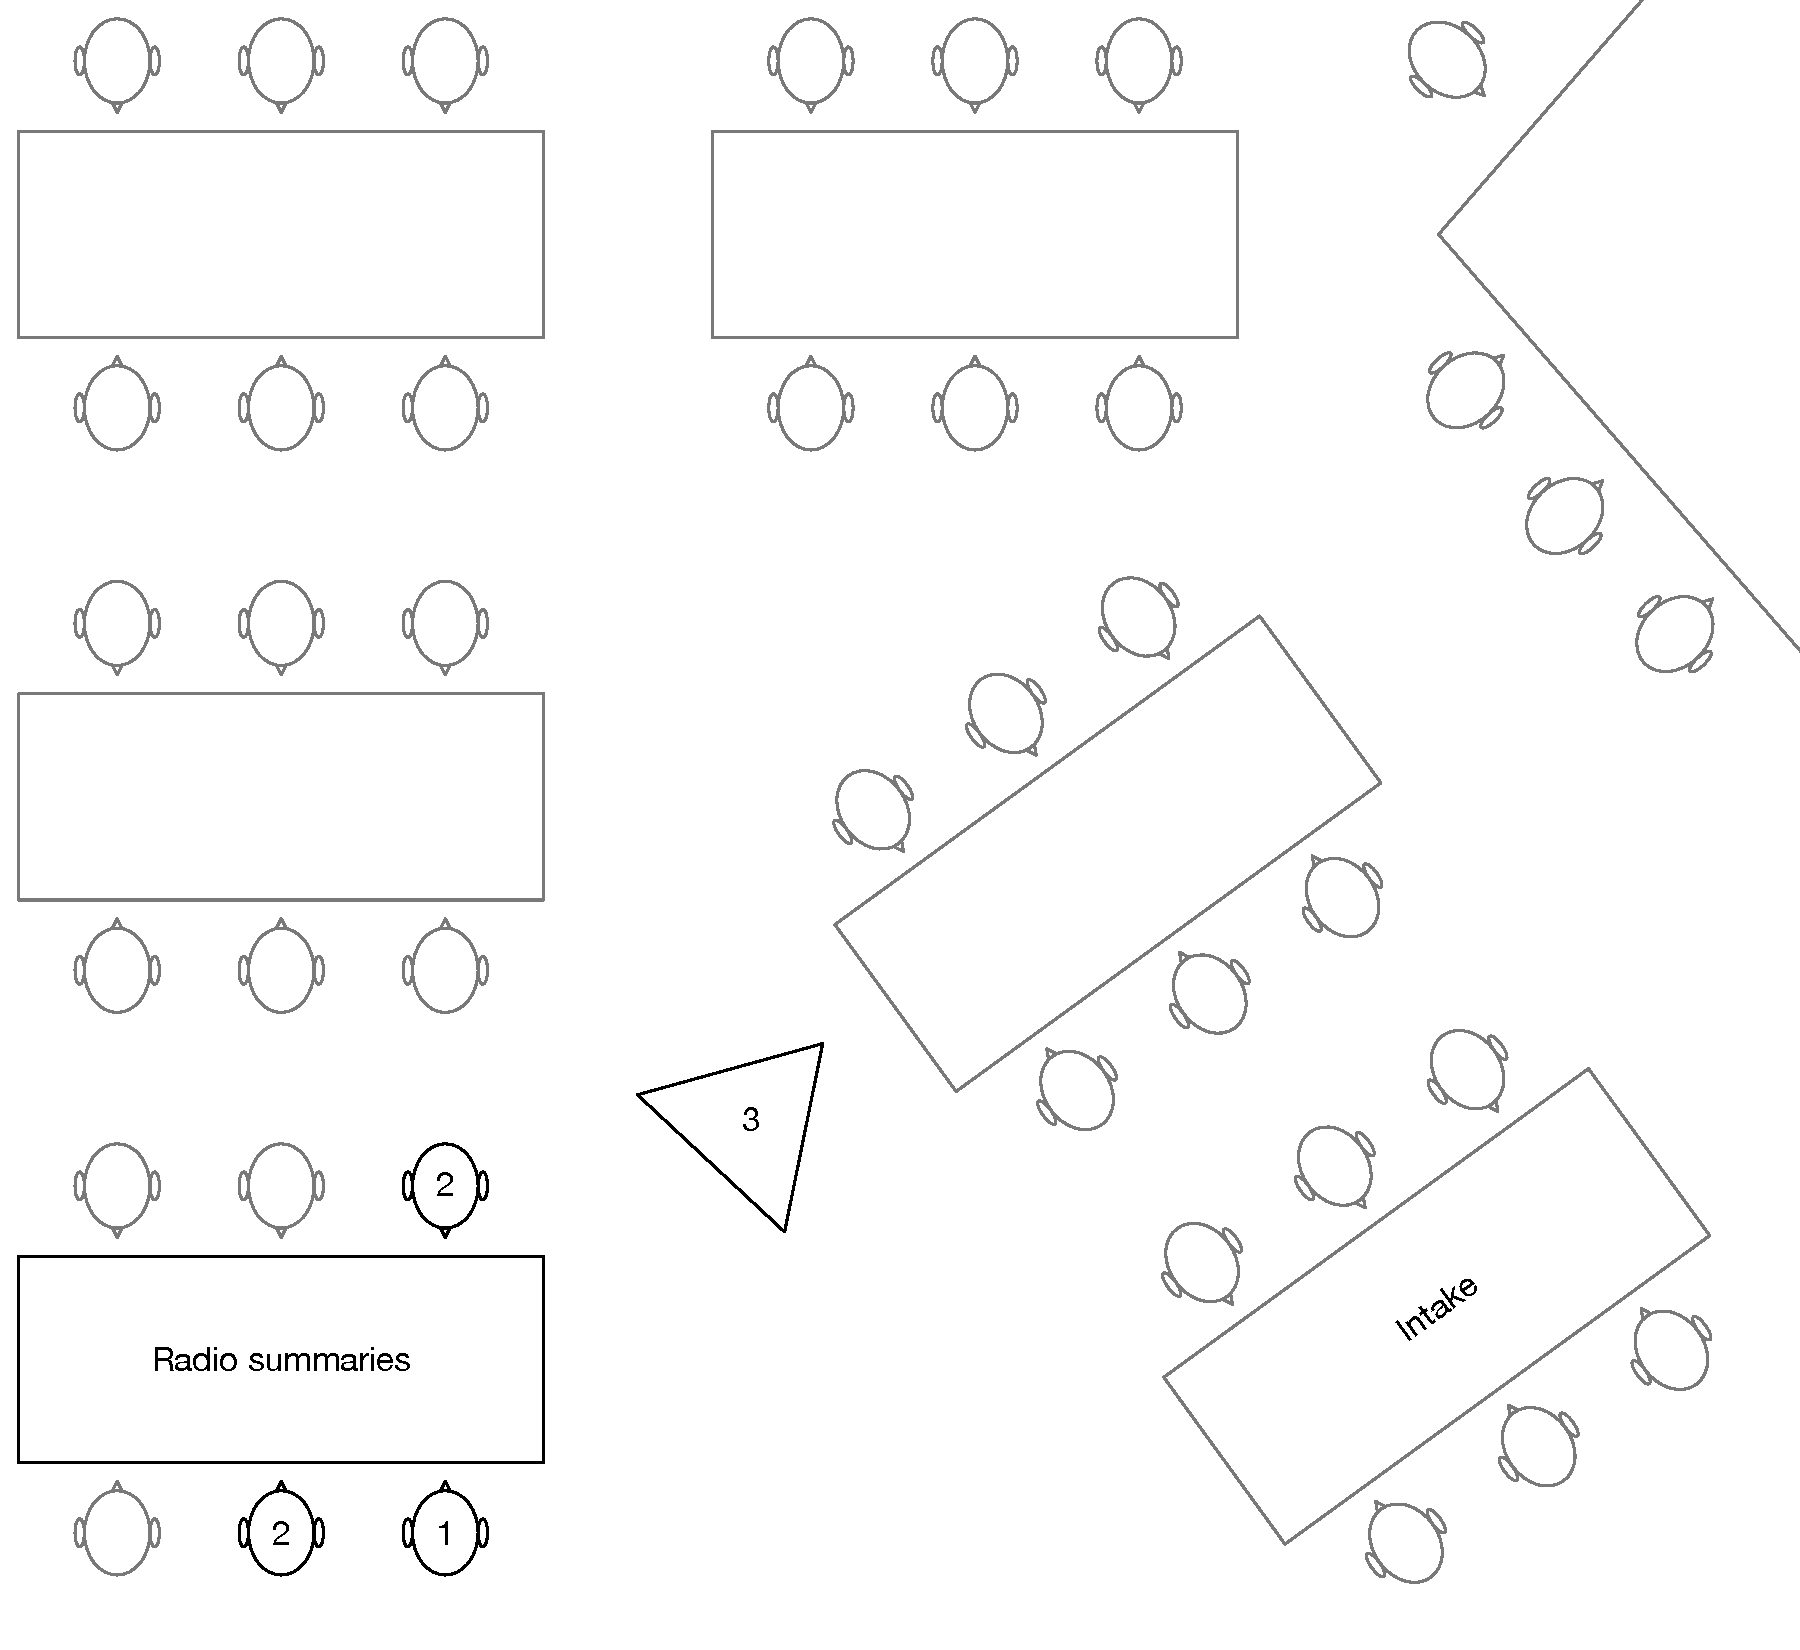
\includegraphics[width=4in]{figs/news-layout.pdf}
  \caption{Layout of radio summaries within the BBC newsfloor, showing the assistant editor (1), broadcast journalists
  (2) and the arrivals board (3).}
	\label{fig:newsroom-layout}
\end{figure}

\begin{figure}[p]
  \centering
  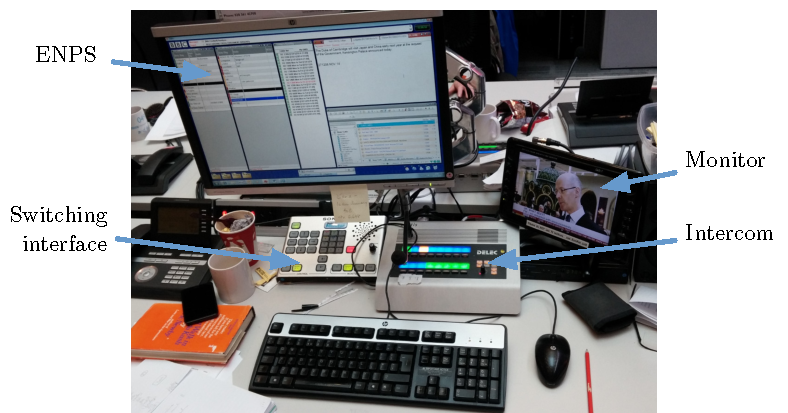
\includegraphics[width=\columnwidth]{figs/news-desk-labelled.pdf}
  \caption{Desk of the radio summaries assistant editor, showing ENPS (1), a switching interface (2) for controlling
  the output of a desktop TV monitor (4) and headphones, and an intercom (3) for communicating with other teams.}
  \label{fig:news-desktop}
\end{figure}

\begin{figure}[p]
  \centering
  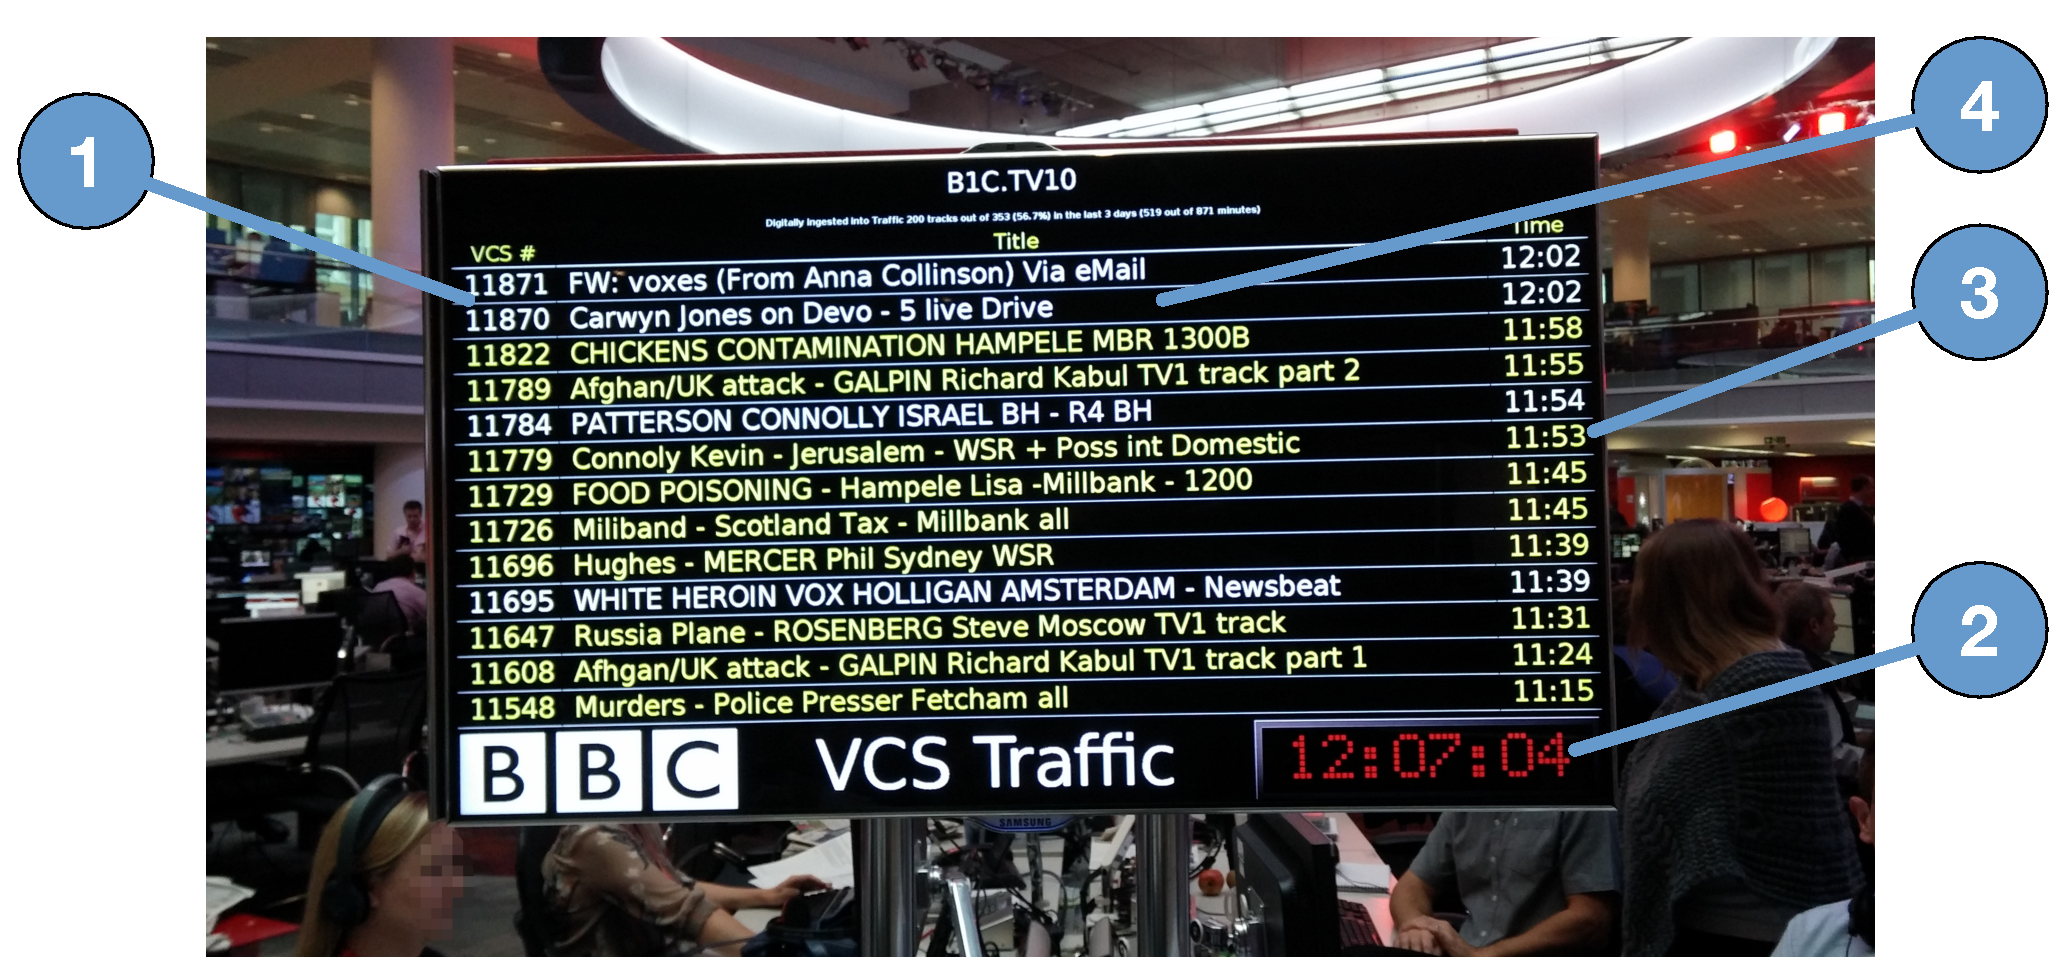
\includegraphics[width=\columnwidth]{figs/arrivals-board-labelled.pdf}
  \caption{Arrivals board in BBC newsroom, showing the ID number (1), arrival time (3) and name (4) of each audio clip.
  The screen also includes a clock (2). ``VCS'' is the colloquial name for the \textit{dira!} radio production system,
  as it is made by a company that used to be called VCS.}
  \label{fig:news-arrivals}
\end{figure}

The broadcast journalists and assistant editor write the summaries on a desktop PC using a software package called
``Electronic News Production System'' (\textit{ENPS}). Figure~\ref{fig:news-enps-edit} shows the ENPS interface. ENPS
is used for writing scripts, compiling and approving news bulletins, and monitoring newswire services\footnote{News
reports provided by global news agencies, such as Reuters and Associated Press}. The system is networked so that any
changes made in ENPS are instantaneously updated for everybody. Audio clips are browsed, imported and edited using a
plugin called Media Object Server (\textit{MOS}), which integrates with the \textit{dira!} radio production system.

\begin{figure}[ht]
  \centering
  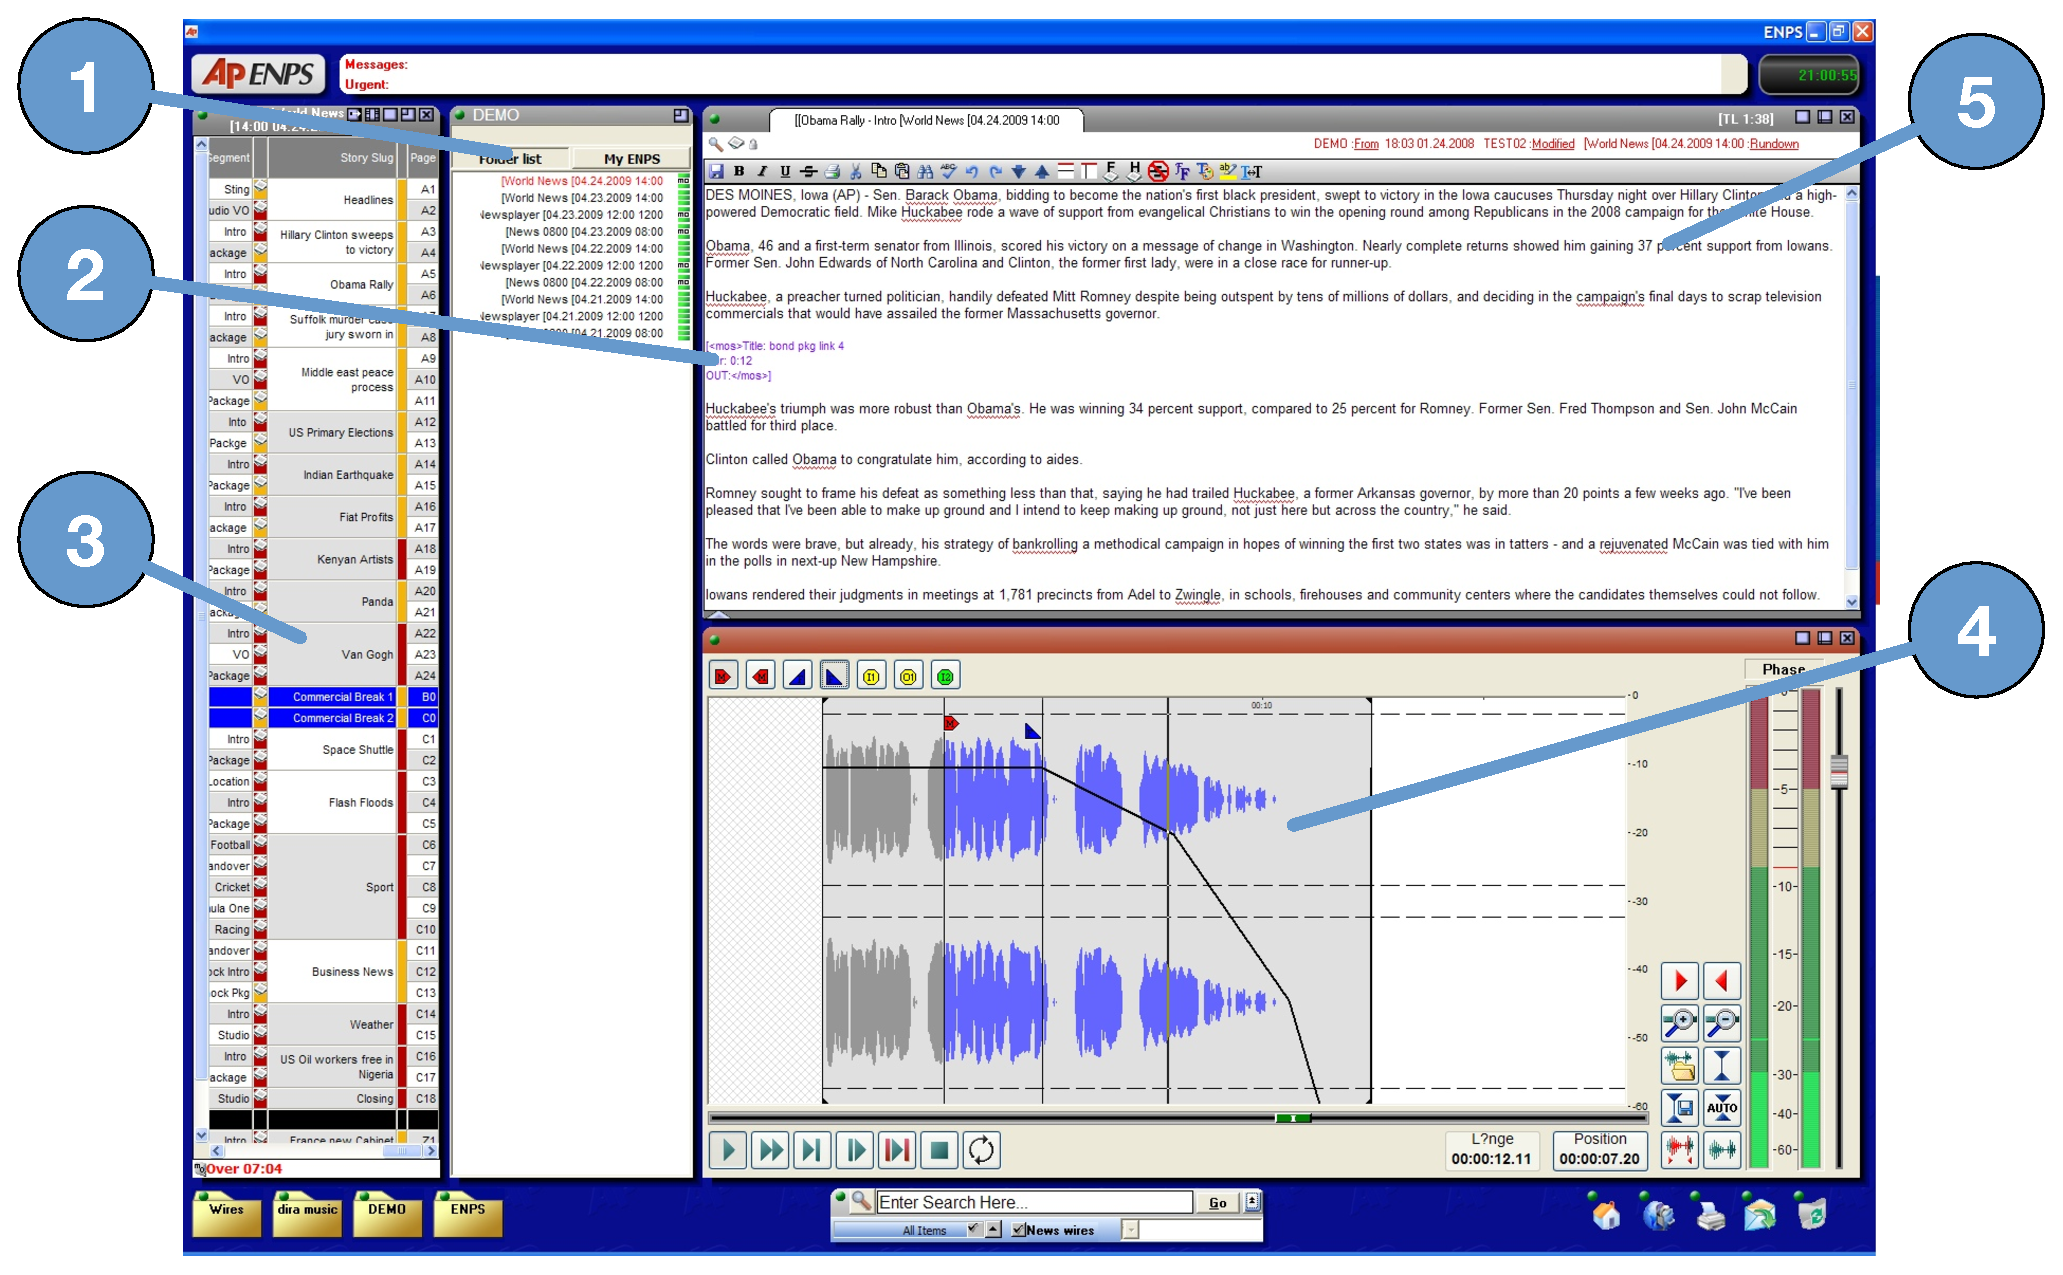
\includegraphics[width=\columnwidth]{figs/news-enps-labelled.pdf}
  \caption{Editing a clip in ENPS, showing the schedule and approval status of the news report (3), the list of drafts
  for each summary (1), the text of the summary currently being edited (5), audio clips inserted into the summary (2),
  and the ``MOS'' plugin for finding and editing audio clips in the \textit{dira!} radio production system}
  \label{fig:news-enps-edit}
\end{figure}

\subsubsection{Task analysis}
Figure~\ref{fig:news-flowchart} shows the operational sequence diagram of the radio summaries production process. A
description of the workflow is written below.

\begin{figure}[ht]
	\centering
	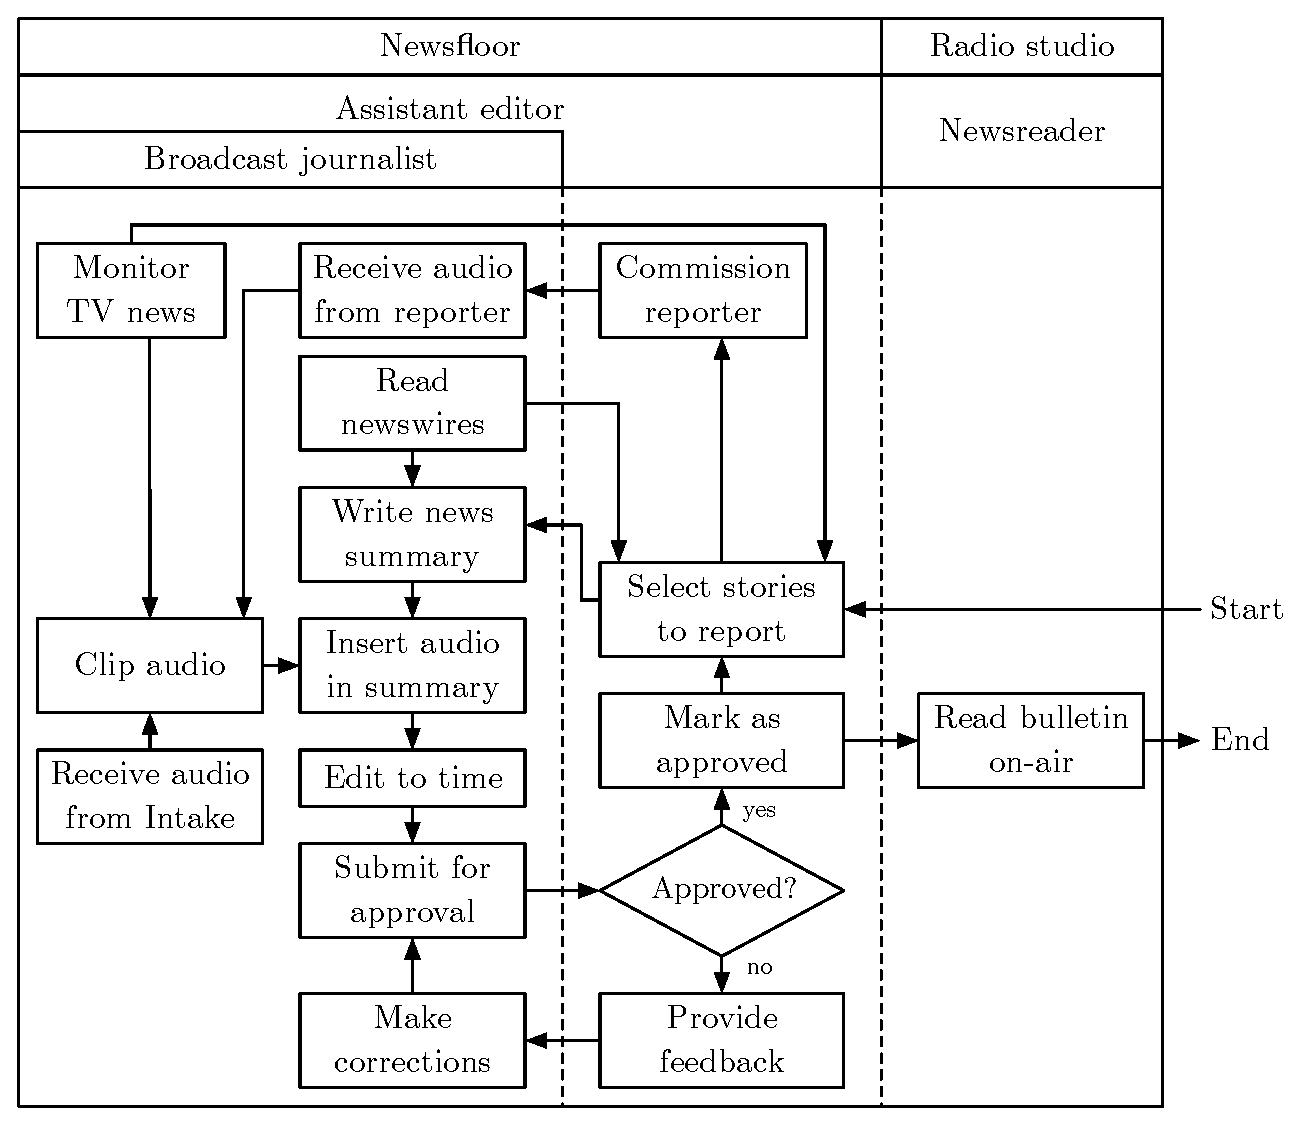
\includegraphics[width=4in]{figs/news-workflow.pdf}
  \caption{Operational sequence diagram of news summaries production, partitioned by role and location.}
	\label{fig:news-flowchart}
\end{figure}

% read newswires
% monitor TV news
% select stories
% commission reporter
% write summary
The assistant editor selects which news stories should be included in the bulletins. The stories come from multiple
sources, including newswire services and the BBC television news channel.  Newswire services are global news agencies
that provide news reports to subscribing news organisations, such as Reuters and Associated Press (AP).  Newswire
reports are accessed through ENPS, and users are notified of any reports flagged as important.  As they work, the
assistant editor and broadcast journalists keeps an eye on the BBC News TV channel using a small monitor on their desk.
They watch the channel to spot any breaking news stories, or material which they could use in their bulletins, such as
interviews.  The assistant editor will sometimes commission a reporter to record a news report for a particular story,
so that they have some quality audio content to include in the summary. The broadcast journalists and assistant editor
both write the summaries for a specific bulletin using ENPS. Previously-written summaries are often re-used, but are
updated to reflect the latest information.

% receive audio from reporter
% receive audio from intake
% monitor TV news
% clip audio
% insert audio
Audio clips are added to each summary to include quotes from interviews and items from reporters. The audio is sourced
from the Intake team, directly from reporters and from the BBC News TV channel. Audio from Intake and reporters is
imported using the \textit{MOS} plugin. This allows users to find audio in the \textit{dira!} radio production system
and edit clips by cutting the audio, and controlling sound levels/fading. Finished clips are inserted directly into the
text of the written summary using a drag-and-drop gesture. At this point, the broadcast journalist gives the clip a
name and can optionally include the ``in/out words'' that are spoken at the start and end of the clip.  The name,
in/out words and duration of the clip appear in the script.  Audio from the BBC News TV channel must be found and
clipped by the broadcast journalist themselves. The sound from the televison channel is automatically recorded into
\textit{dira!} in 40-minute segments. The broadcast journalist uses the \textit{MOS} plugin to browse to the desired
segment, find the location of the audio they want, and create a clip of the audio.

% edit to time
% submit for approval
% provide feedback
% make corrections
% read bulletin on-air
The finished bulletin must fit an exact time slot (e.g. two minutes), so the broadcast journalist must estimate how
long it takes to read their bulletin and edit the text to the correct length.  When a journalist has finished writing
their bulletin, it is placed into the `running order' and named according to the network and time (e.g. `R4 Thu
10:00').  The assistant editor then reviews the bulletin and listens to the clips. This is to ensure the bulletin is of
the right length, is factually accurate, uses the correct language, and complies with BBC editorial policy and Any
required changes are made either by giving feedback to the journalist, or by the assistant editor making the changes
themselves.  When the item is approved in ENPS, it is labelled with a green flag, which indicates that it has been
signed-off.

The newsreader sits in a radio studio and normally has no direct contact with the summaries team.  At the time of the
news bulletin, the newsreader reads the script directly from ENPS while on-air. The audio clips in the script are
automatically loaded into the play-out system, and the newsreader uses a button to trigger them at the right time.  The
duration and in/out words of the audio clip are displayed in the script, which helps the newsreader to predict when the
clip ends.

\subsubsection{Challenges}

The summaries team work under high-pressure circumstances. They have less than an hour to put together several minutes
of content that will be read to millions of listeners. News can break at any moment, so sometimes bulletins need to be
changed or re-written minutes before they are broadcast. In addition to these pressures, it is very important that the
news reports are factually accurate and balanced.  Due to these circumstances, the particiants had very little time to
talk to the researcher. During observation, all of the communication between team members was directly related to the
task at hand, and there was no chatting or socialising.

When creating clips from television broadcasts, the broadcast journalists must source the clips from 40-minute-long
segments.  To find the audio, they would seek through the recording, listening for a particular voice or mention of the
topic of interest.  The \textit{MOS} plugin interface they used displayed a waveform, but this did not seem to help
them find the audio.  This made finding and cutting clips a time-consuming and difficult task, particularly when
performed under pressure.  Application of segmentation or speech-to-text technology could help by indicating where
people are speaking, displaying keywords that are mentioned, or allowing the recording to be searched by text.

The bulletins written by the broadcast journalists must target a specific duration for when they are broadcast. It is
difficult for them to write and edit the script so that it contains all the facts, is balanced and reads well while
hitting the correct duration. However, in addition to this, they have no indication of how long it takes to read a
piece of text. They must therefore estimate this based on experience, or reading it in their head.
By developing a system that estimates the duration of spoken text, broadcast journalists may be able to target a
specific duration more efficiently. 

When it comes to inserting clips into the script, in and out words must be manually entered so that the clip can be
recognised, but there is not enough time to transcribe the whole clip.  Speech-to-text technology would be able to
automate this and full transcription could further help the journalists to recall the clip and write the script around
it.

\subsection{Drama}\label{sec:drama}
Radio 4's ``15 Minute Drama'' is a series of original drama and book dramatisations, broadcast twice-daily. Production
of drama is very different from most other genres in radio, as it is based on a pre-written script of a radio play. The
drama is created over several weeks. The researcher observed the production over two full days -- one for the recording
of the drama and the other for the editing process.  The observation did not include the writing of the script.

\subsubsection{Roles and responsibilities}
The production team is led by a \textit{director} who works with a \textit{broadcast assistant} and three studio
managers (SMs) -- a \textit{panel SM}, \textit{grams SM} and \textit{spot SM}. The team record a \textit{cast} of
actors who perform the drama.

The director is responsible for leading the team and making editorial and creative decisions. Before the recording,
they will have commissioned a writer to create the script, and worked with them to refine it. During the recording,
they announce the start and end of takes, and give feedback to the cast about their performances.  They also work with
the SMs to ensure the drama has the right sound.

The director is supported by a broadcast assistant who handles much of the administrative work before and after the
recording, such as making copies of the script, booking the cast, producers and rooms, and processing payments.
During the recording, they annotate the script with detailed notes about the position and length of each take, and mark
any mistakes or re-takes.

The panel SM is responsible for the sound of the drama. They lead the other two SMs during the recording process and
operate the mixing desk in the cubicle. They work with the spot SM to position the actors and microphones to achieve
they sound they want. They also make a backup recording of each performance onto CDs. After the recording, they work
with the director to edit the drama into the final version.

The grams SM prepares and plays pre-recorded sound effects during the recording, and is also responsible for recording
the performances using a DAW.  ``Grams'' refers to gramophones, which were historically used to play pre-recorded sound
effects.  After each take, the grams SM labels the recording with the episode, scene and take numbers, which are later
used to assemble the final programme.  When the director wants to listen back to a performance, the grams SM uses the
DAW to find and replay the desired take.

The spot SM works in the studio, rather than the cubicle, where they set up and position microphones and create spot
effects, also known as ``foley'' in the movie industry. The effects are produced using a large variety of props that
are kept in the studio to emulate common effects such as doors, windows, locks, telephones and footsteps to name a few.

The cast are hired by the director specifically for the drama being recorded. Often the cast are sourced from the BBC
Radio Drama Company (RDC), which is a rotating group of actors that are employed by the BBC. The cast perform the
radio play in the studio, working under instruction from the director.

\subsubsection{Environment and tools}
The drama we observed was recorded in Studio 60A, which is a purpose-built flexible performance space at BBC New
Broadcasting House in London. The studio contains spaces with different acoustic properties, including movable
absorbers and a foam-lined spiral corridor that used to simulate distance. There are many fixtures and props for
re-creating common environmental sounds including freestanding doors/windows with a variety of knockers and letter
boxes, a staircase with wood, concrete and carpet steps, an upstairs bedroom and a fully working kitchen.  In addition,
there are a wide range of props that are used to create spot effects.  The studio is a large space, so there are four
CCTV cameras which are used to allow the producers in the cubicle to see parts of the studio that are out of view. 

The studio is connected by a large acoustically-isolated window to the cubicle where the production team sit.
Figure~\ref{fig:drama-studio} shows the view of the studio from the cubicle, and Figure~\ref{fig:drama-layout} shows
the layout of the spaces. The mixing desk is operated by the panel SM and is positioned directly in front of the
window.  The broadcast assistant sits to the right of the panel SM and the director sits directly behind them. The
grams SM sits at the back of the room, while the spot SM spends most of their time in the studio.
%TODO Intercom

The panel SM sets the sound levels and balances the audio using the mixing desk, and makes a backup recording of the
performances using a CD recorder located in a rack to the left of the mixing desk.  Under the mixing desk, there is a
foot pedal which controls a light in the studio to silently indicate the start of a performance, known as a ``cue
light''. The panel SM also controls warning lights displayed above the door to the studio to stop people from walking
in mid-performance.  The grams SM uses software called ``SpotOn'' to select and play pre-recorded sound effects. They
use the ProTools DAW to record each performance, and label them with the episode, scene and take numbers.

Figure~\ref{fig:drama-edit} shows the editing suite where the panel SM and director perform the post-production work.
The editing suite is a compact acoustically-treated room which houses a PC running ProTools, stereo speakers, a small
mixing desk and level meters.  The left monitor is used to find pre-recorded sound effects and the right monitor is
used to arrange and edit the drama recordings. The panel SM uses an annotated copy of the script to guide their
editing.

\begin{figure}[p]
  \centering
  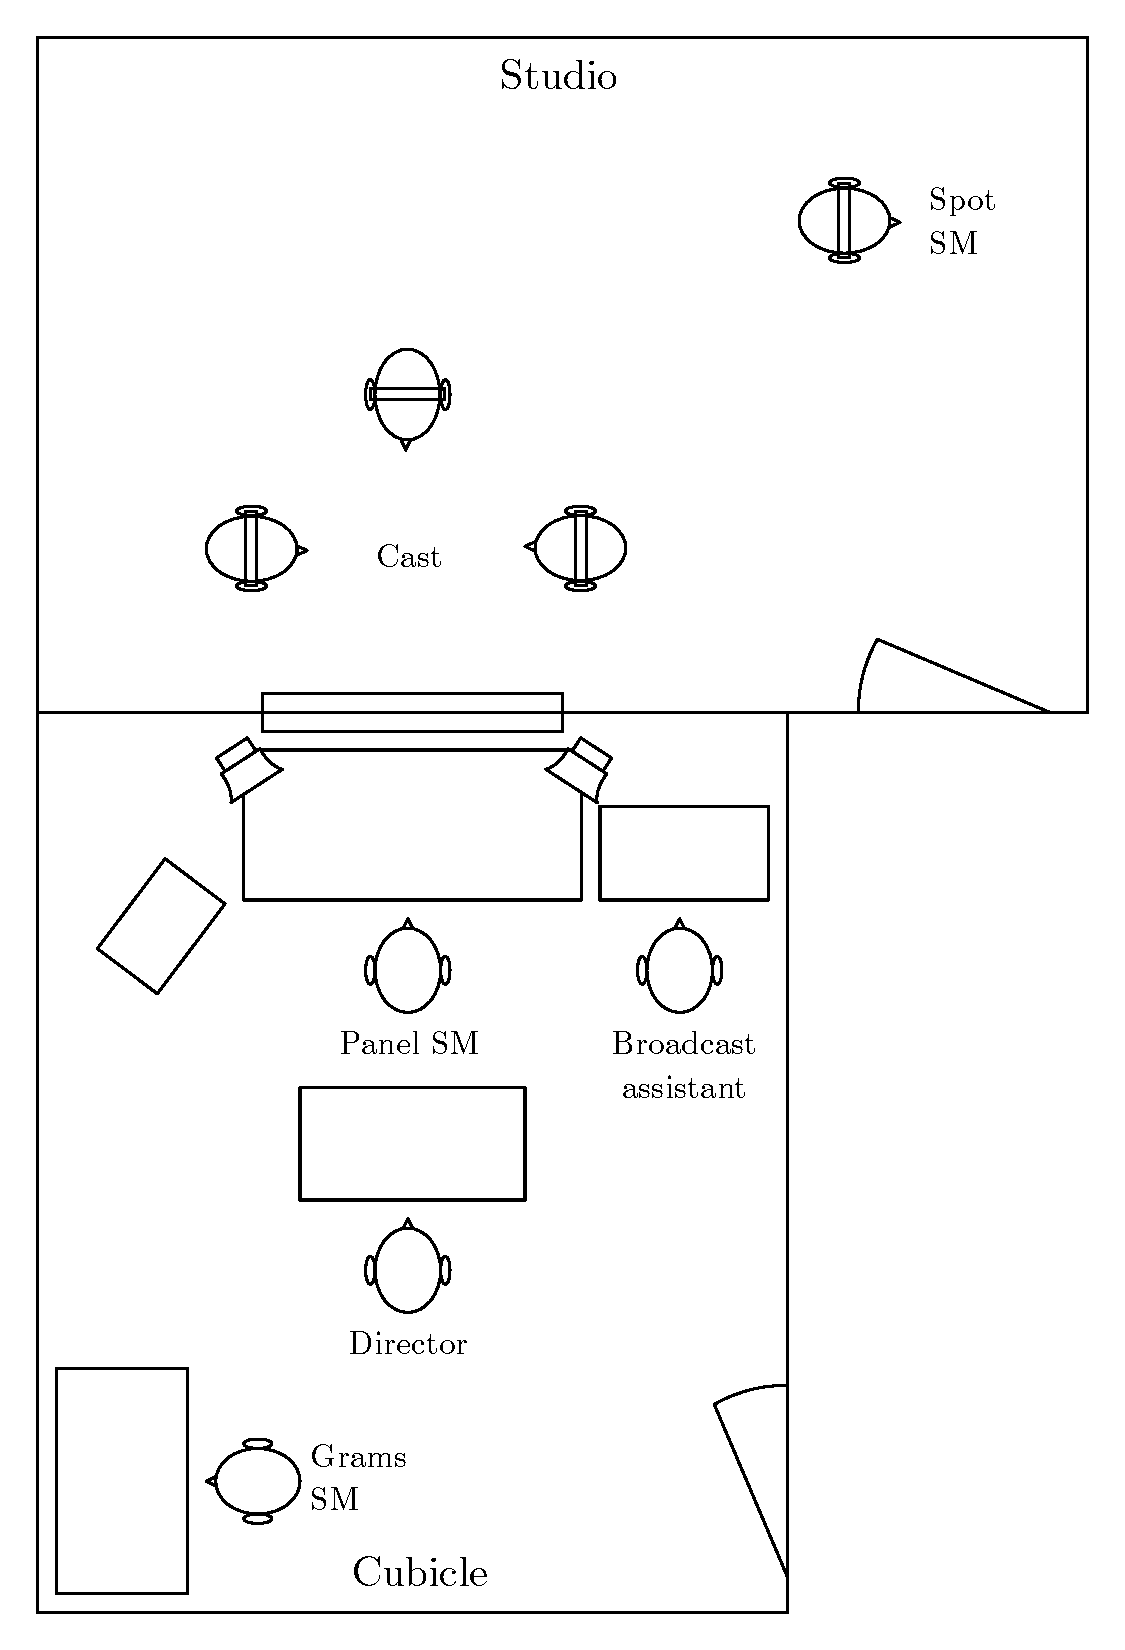
\includegraphics[width=3.5in]{figs/drama-layout.pdf}
  \caption{Physical layout of the drama studio and cubicle, showing the director (1), broadcast assistant (2), cast
  (3), panel SM (4), grams SM (5) and spot SM (6).}
  \label{fig:drama-layout}
\end{figure}

\begin{figure}[p]
  \centering
  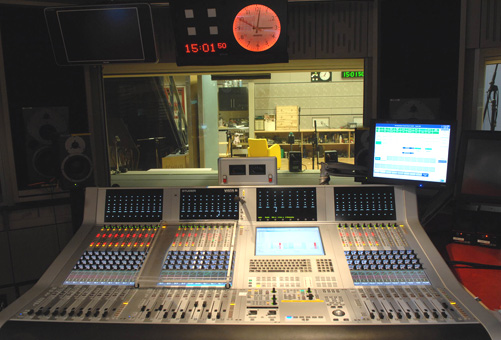
\includegraphics[width=\columnwidth]{figs/60a.jpg}
  \caption{Cubicle of studio 60A.}
  \label{fig:drama-studio}
\end{figure}

\begin{figure}[p]
  \centering
  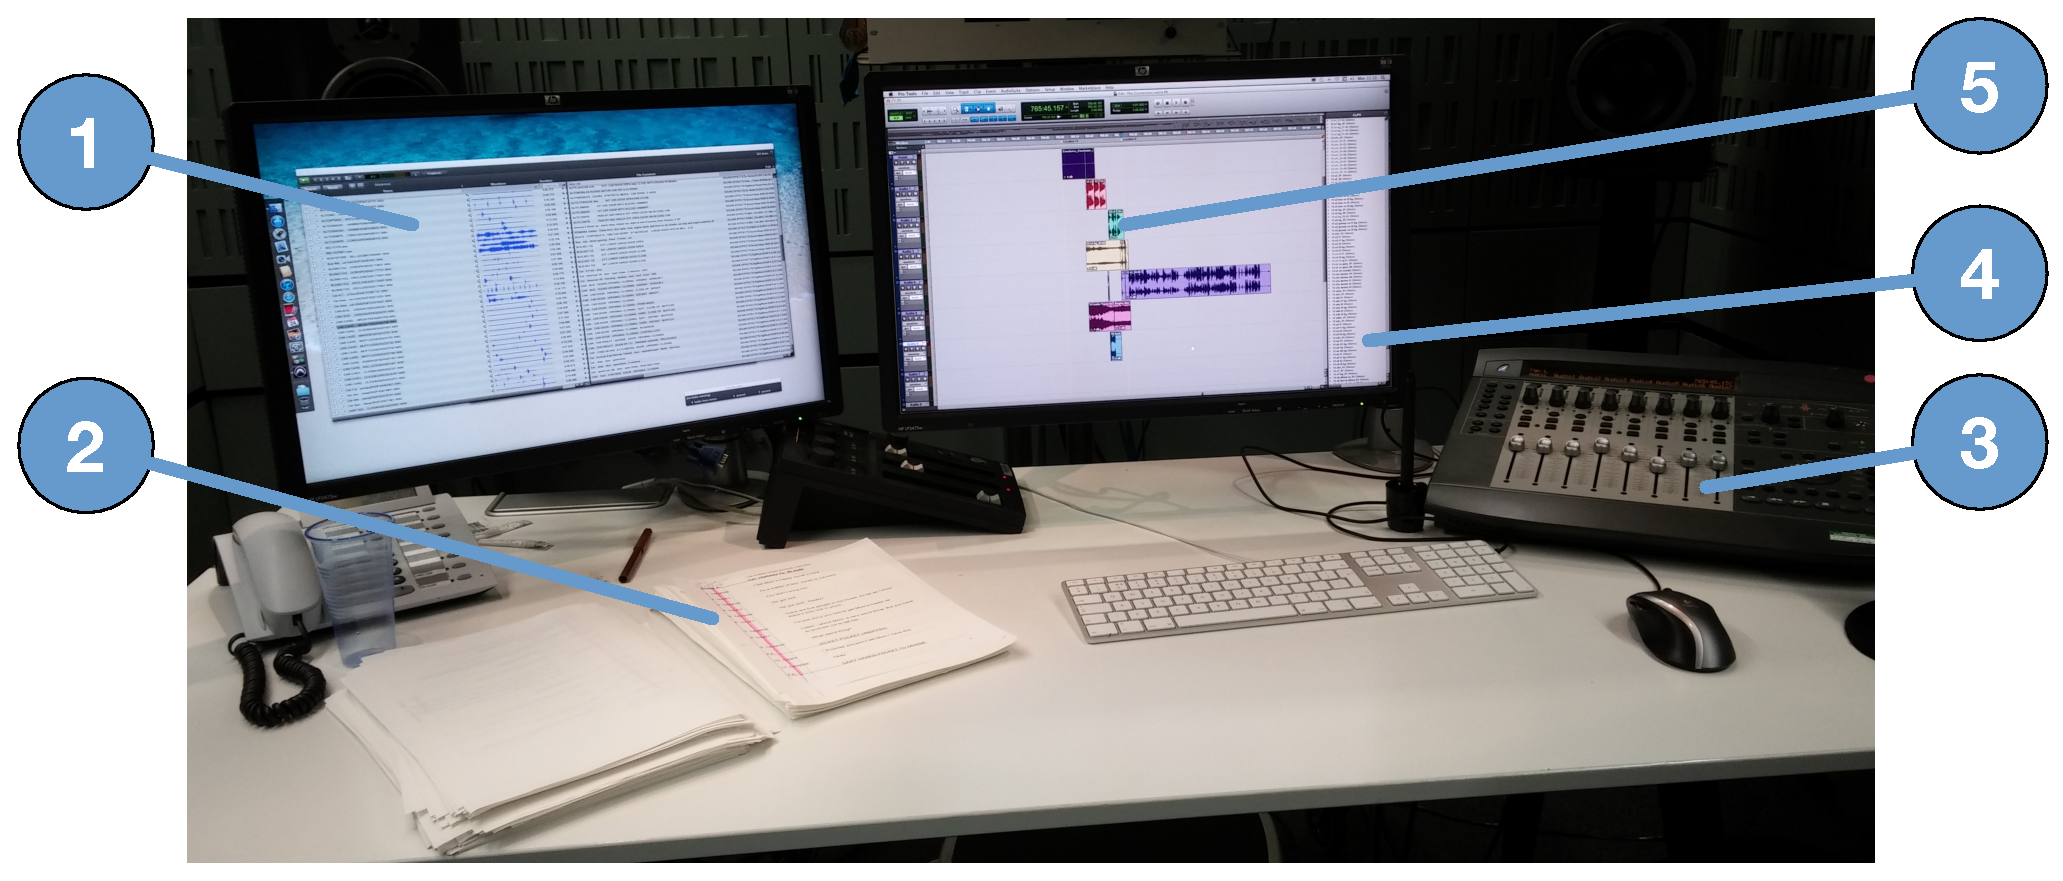
\includegraphics[width=\columnwidth]{figs/drama-edit-labelled.pdf}
  \caption{Radio drama edit suite, showing the sound effects library interface (1), the annotated script being edited
  (2), a mixing desk (3), the ProTools DAW with a list of recorded and labelled audio clips (4) and the edit time-line
  (5), and level meters (6).}
  \label{fig:drama-edit}
\end{figure}

\subsubsection{Task analysis}
Figures~\ref{fig:ethno-drama-recording} and \ref{fig:ethno-drama-editing} show the operational sequence diagrams of the
radio drama recording and editing process, respectively. Descriptions of each workflow are presented individually
below.

\begin{figure}[p]
  \centering
  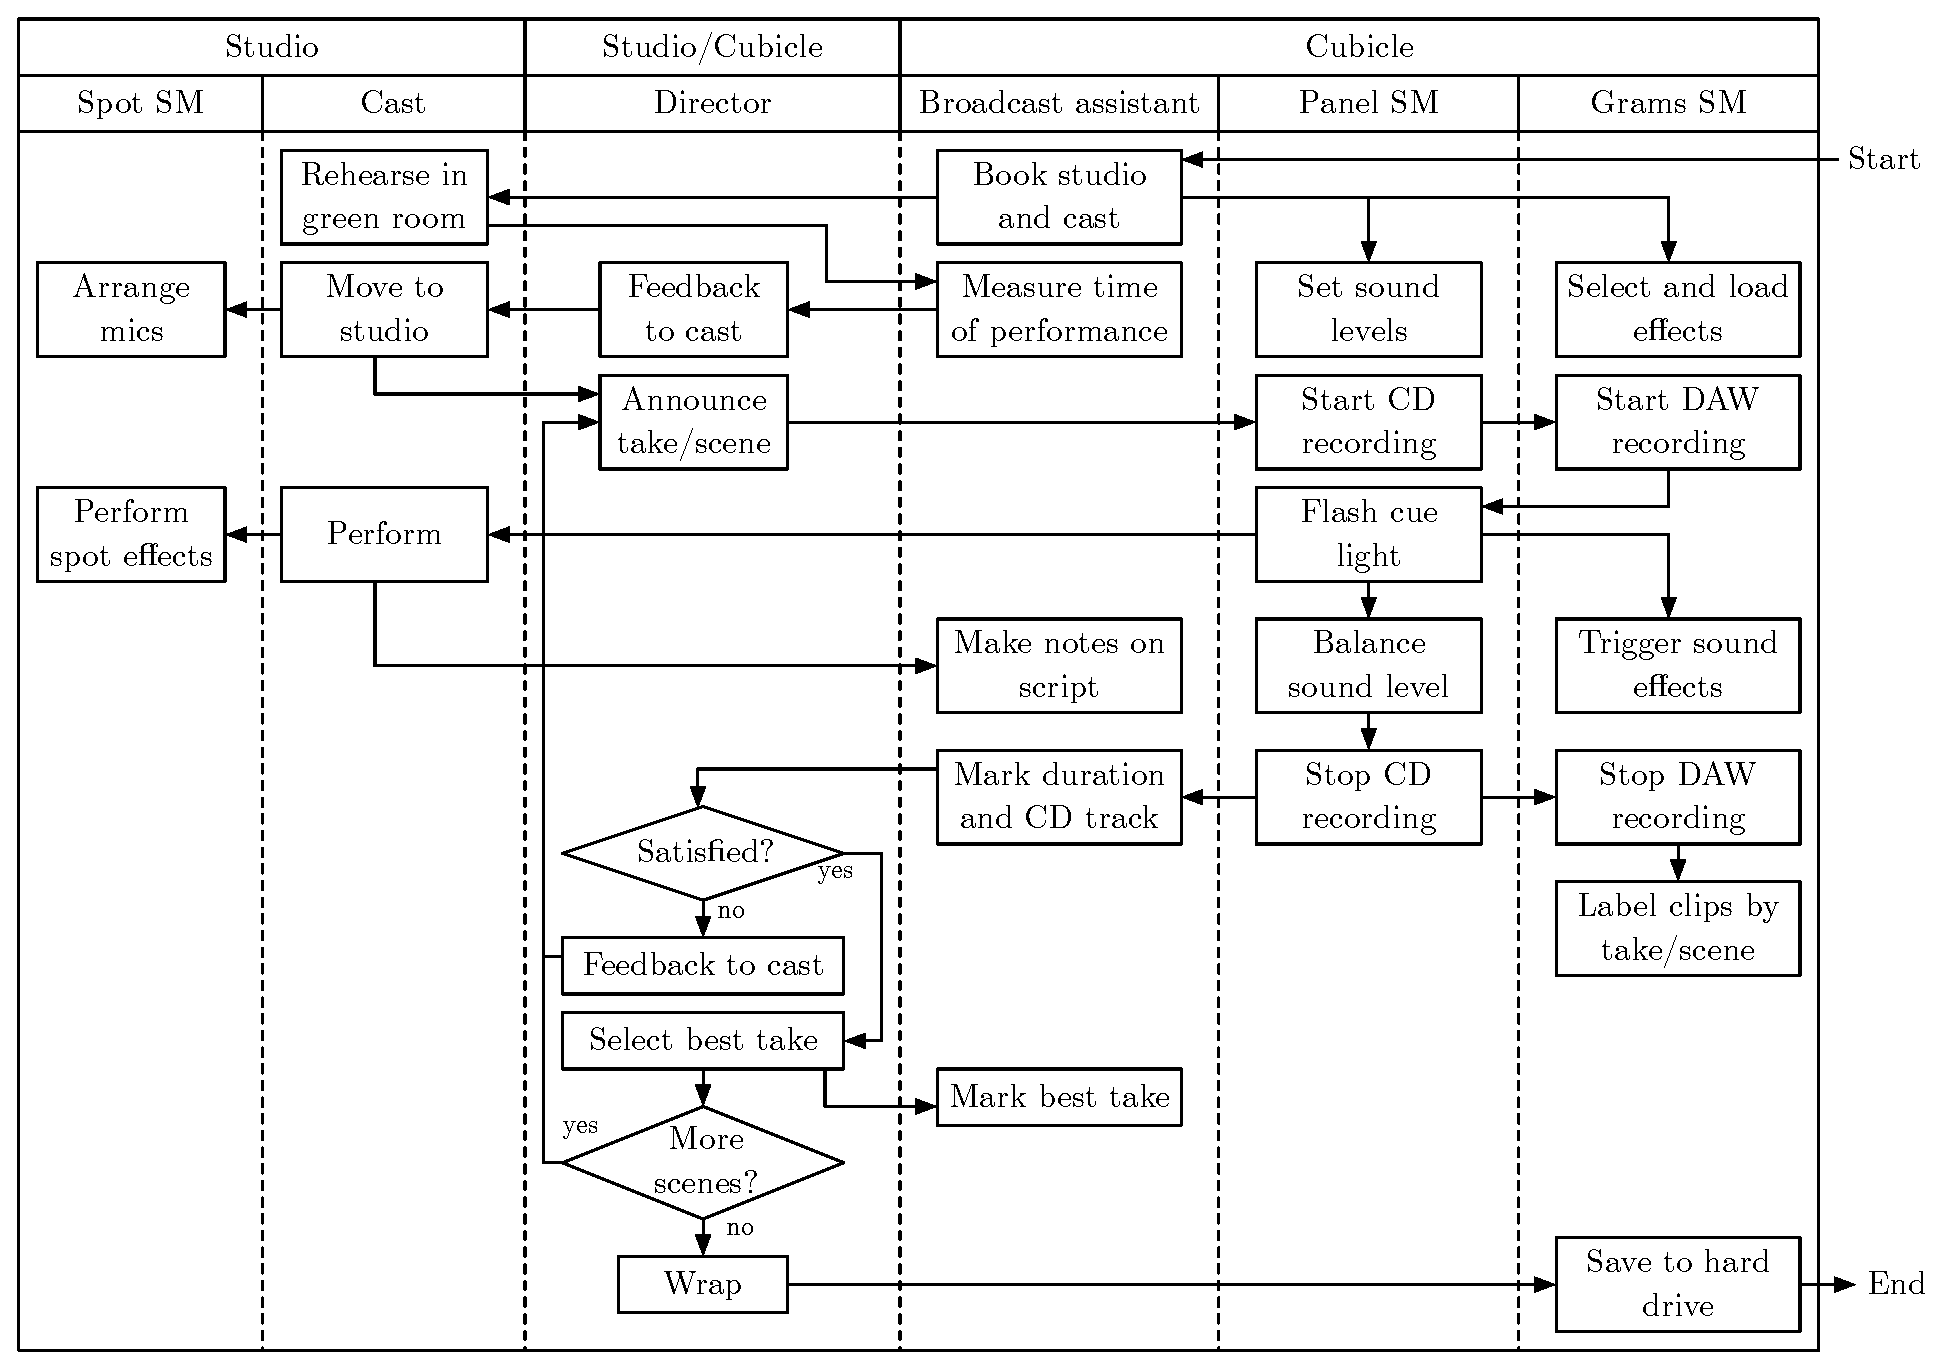
\includegraphics[width=5in]{figs/drama-recording-workflow.pdf}
  \caption{Operational sequence diagram of radio drama recording, partitioned by role and location.}
  \label{fig:ethno-drama-recording}
\end{figure}

\paragraph{Recording}
The recording process involves the entire production team and cast. Between one and two episodes are recorded in a day.
Prior to recording, the cast will assemble in the ``green room'' with the director and rehearse the play. During the
rehearsal, the broadcast assistant measures how long the performances take, to ensure they are not too long or too
short.  The director provides feedback to the cast on their performances before they move to the studio.

The drama is recorded as a series of ``takes''. Each take is a short segment of a scene in an episode, often only
20--30 seconds long.  Multiple takes of the same material are recorded so that the director can give feedback to the
cast on how they would like it to be performed.  The director starts the process by announcing the episode, scene and
take number.  The panel SM starts the backup recording, and the grams SM starts the DAW recording. When everything is
ready, the panel SM flashes the cue light, which signals the cast to start performing.  During each take, everybody 
listens to the performance. The panel SM balances the audio levels, the grams SM triggers pre-recorded sound effects,
and the spot SM performs live spot effects in the studio.

The broadcast assistant make notes on a spreadsheet about the takes and their duration. They also annotate a printed
script with information about each take.  Figure~\ref{fig:drama-script} shows an example of an annotated drama script.
The start and end of each take is marked with a vertical line on the side of the page. The take and backup CD numbers
are written at the top of each line, and the duration of the take is written at the bottom.  If the take starts again
during a recording, the line continues back to the top.  The best take for each scene is marked by highlighting the
line for that take.  Words that are spoken incorrectly are underlined, and repeated words or phrases are marked with
square brackets.  Different coloured pens are used to distinguish the marks for each take.  If multiple brackets
overlap, their order is labelled with numbers.

\begin{figure}[p]
  \centering
  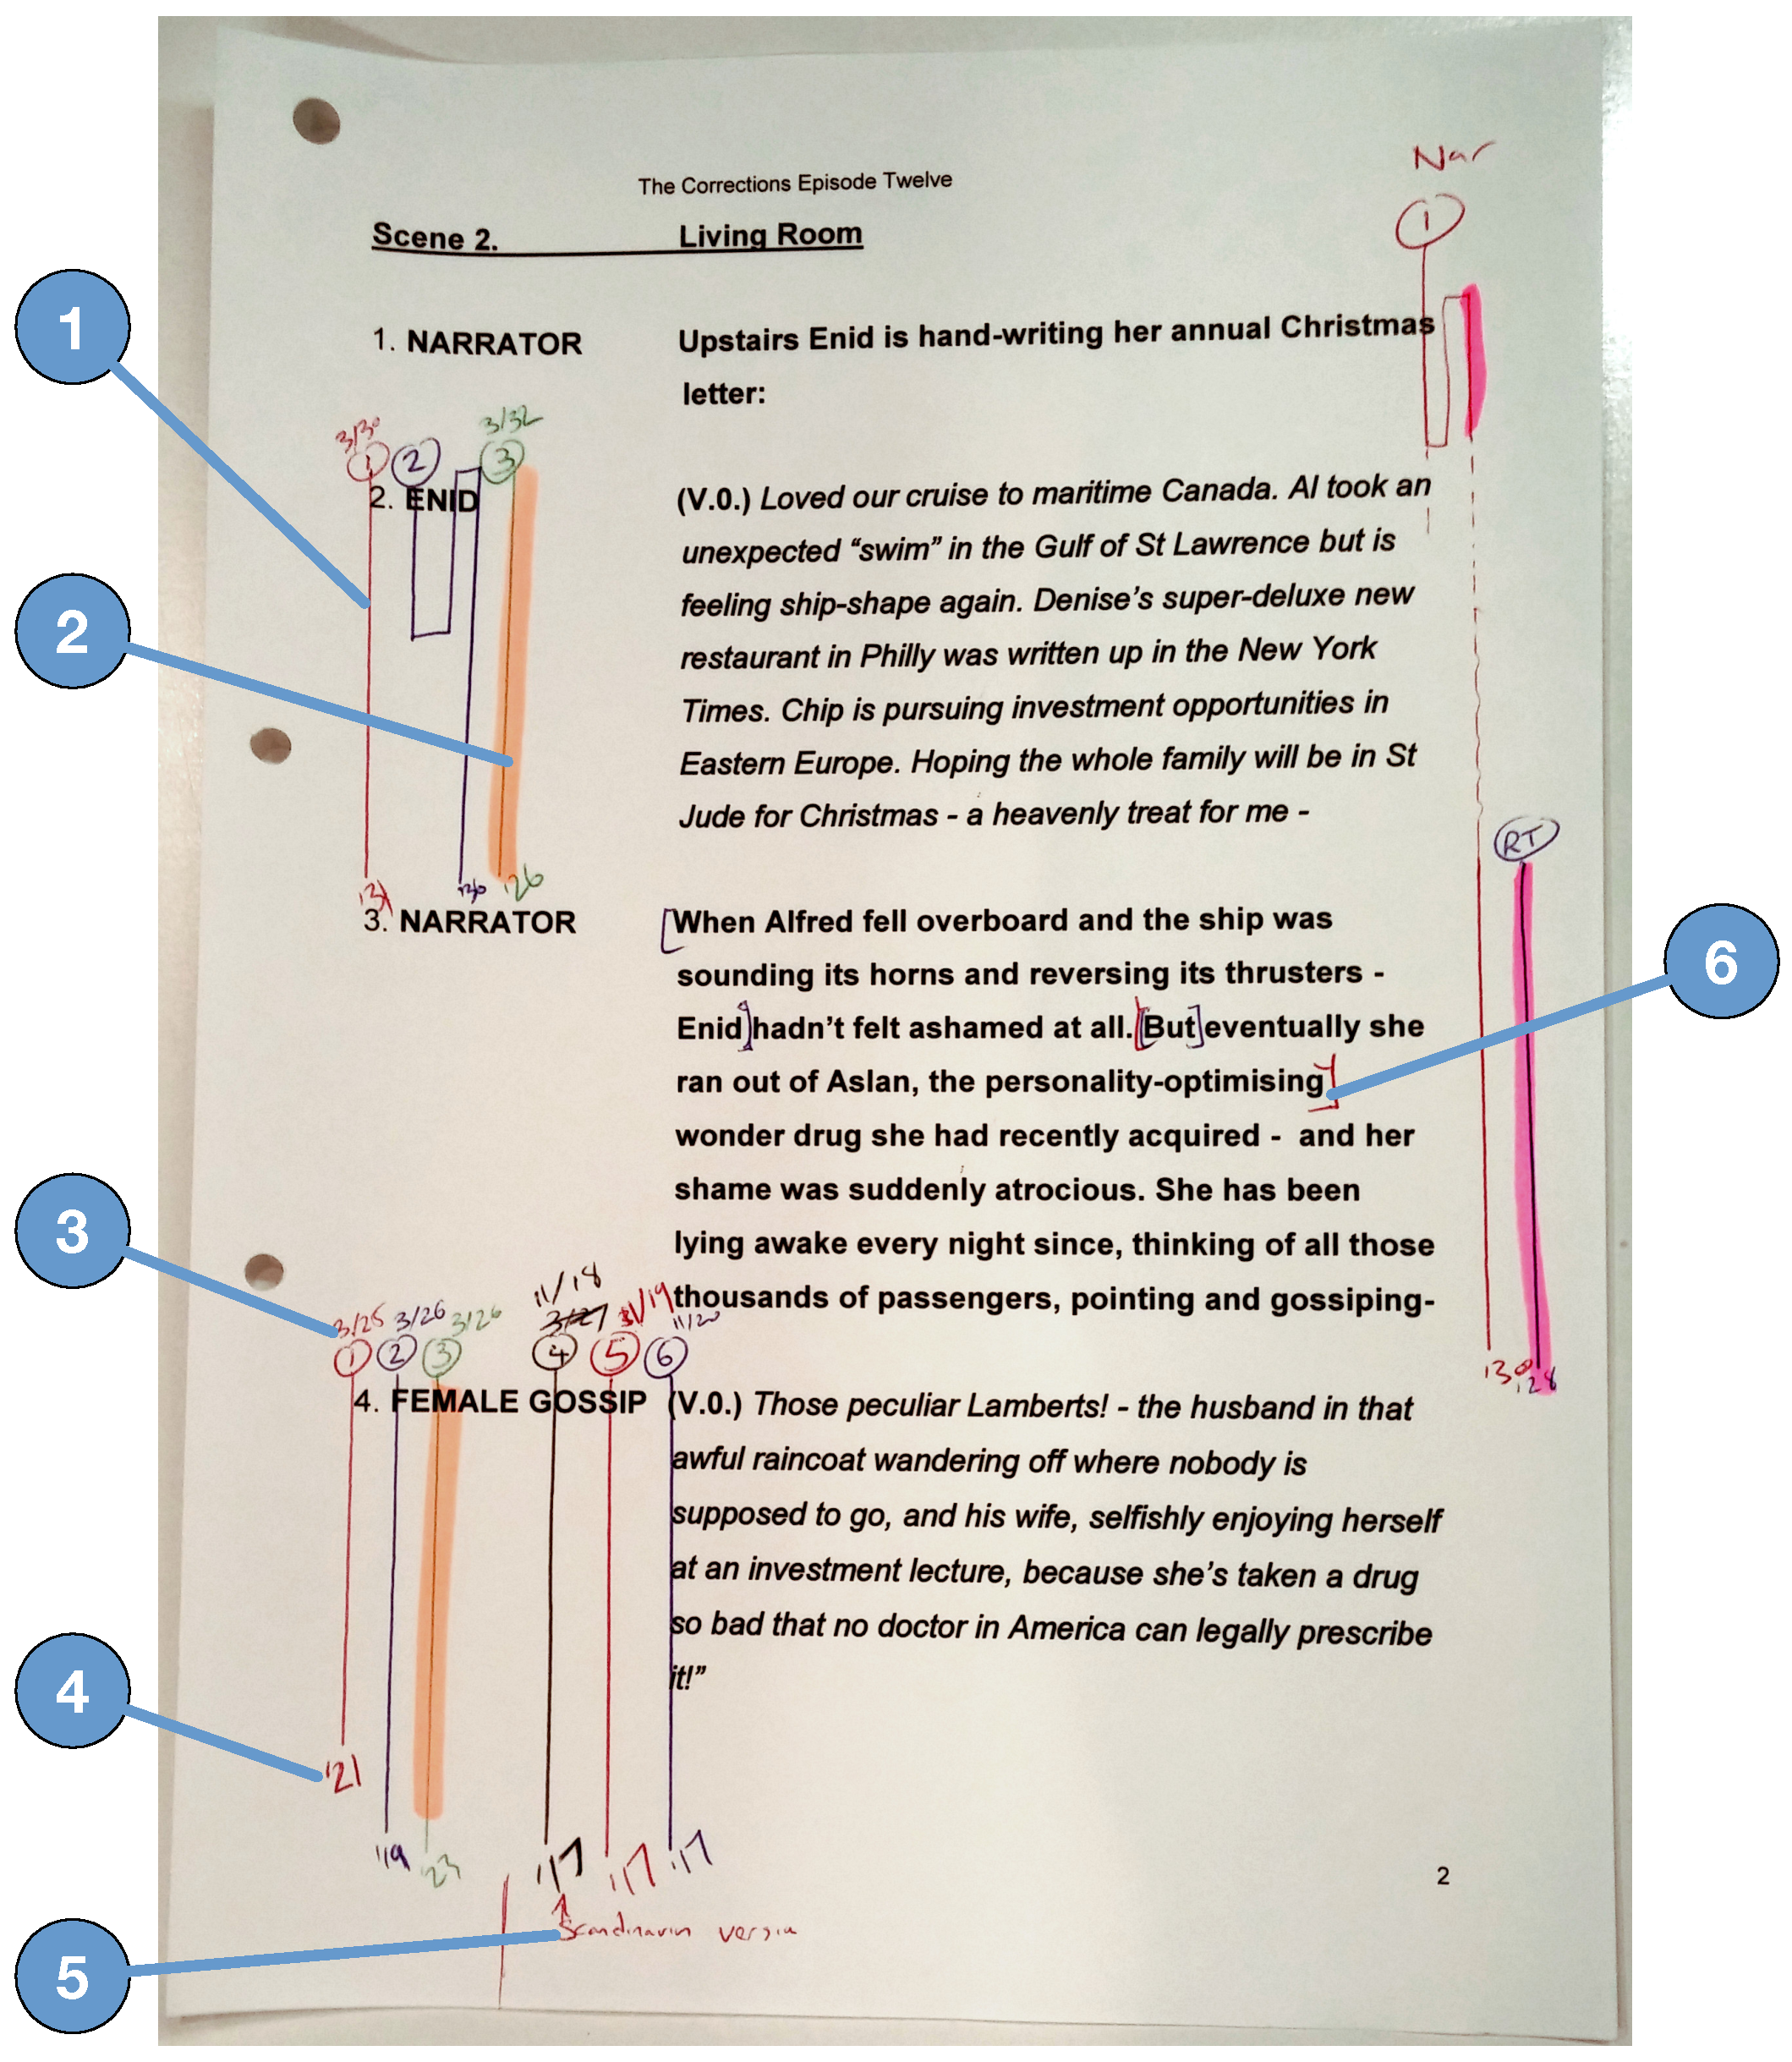
\includegraphics[width=\columnwidth]{figs/drama-markup-labelled.pdf}
  \caption{An annotated drama script page. Recordings for each take are marked with different colour lines (1). The
  best takes are marked with a highlighter pen (2). The backup CD and track number are marked at the top of each line
  (3) and the length of the take is marked at the bottom (4). Notes are often attached to takes (5). Repeated lines are
  marked using square brackets in the colour of the take (6).}
  \label{fig:drama-script}
\end{figure}

At the end of a take, the DAW and backup recordings are stopped. The grams SM uses the DAW to label the clip with the
episode, scene and take number (e.g. e2s3t1). The broadcast assistant marks the printed script and spreadsheet with the
duration of the take and the backup CD number.  If the director is satisfied that they have recorded what they need,
then they select the best take and move onto the next scene. The broadcast assistant marks the best take on the script
and spreadsheet. If the director wants to record another take, they discuss the performance with the production team,
then provide the cast with feedback, either by walking into the studio, or using the intercom.

When the recording is complete, the team either move onto a new episode, or the director sends everybody home.  The
grams SM copies the audio clips from the DAW onto a portable hard drive.  Portable hard drives are used as they can
handle large file sizes better than than the local computer network.  The portable hard drive and annotated drama
script are given to the panel SM.

\begin{figure}[ht]
  \centering
  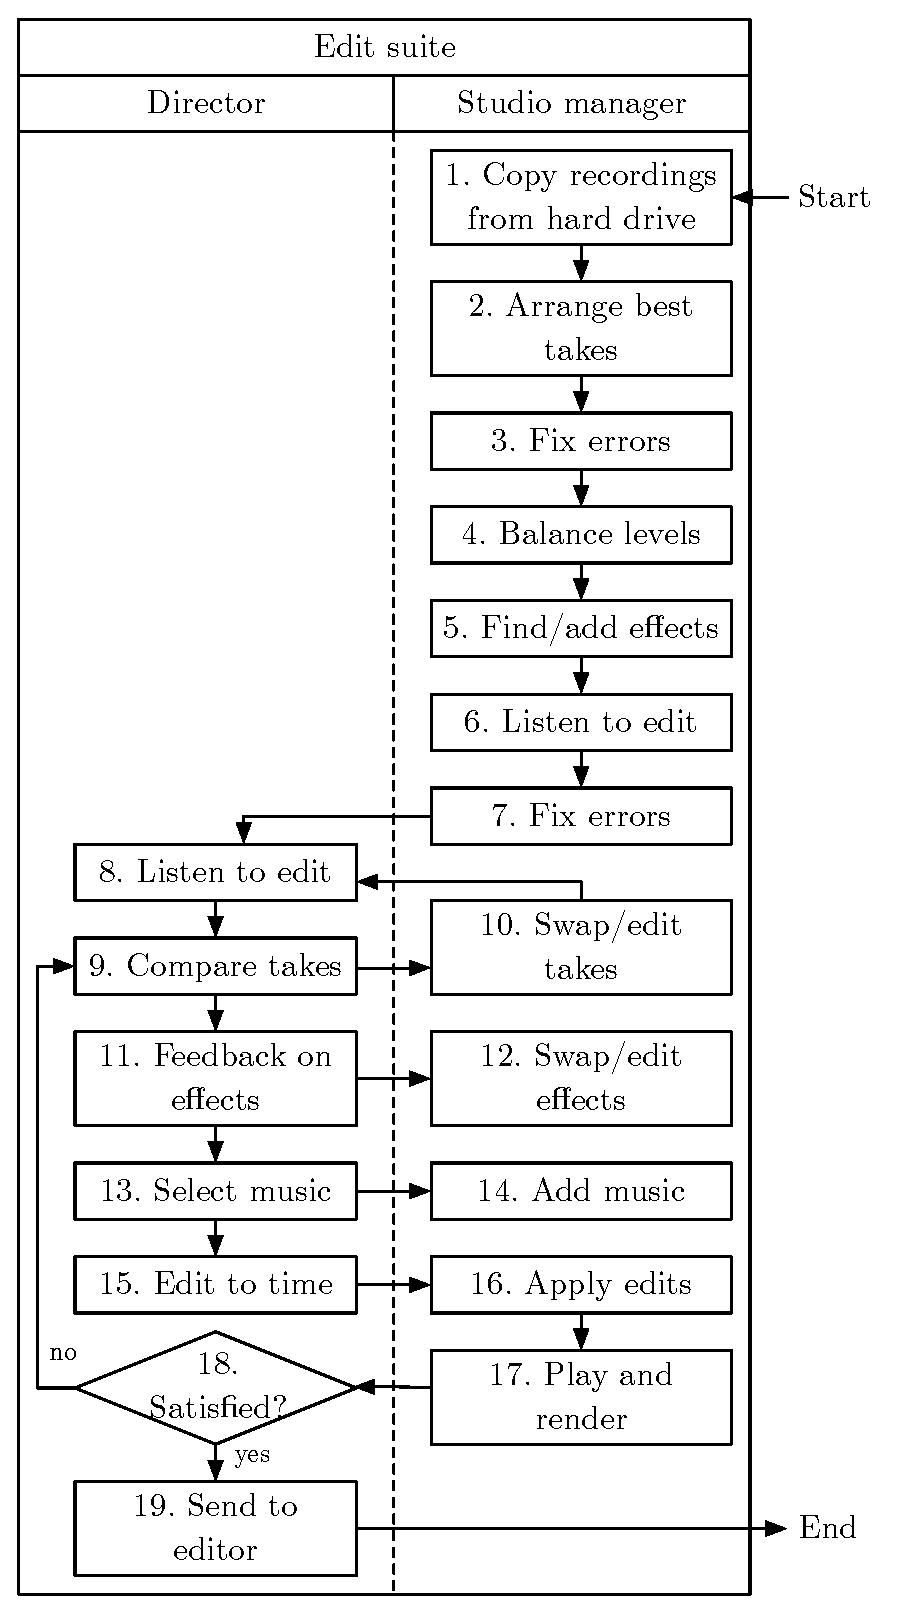
\includegraphics[width=2in]{figs/drama-editing-workflow.pdf}
  \caption{Operational sequence diagram of radio drama editing, partitioned by role and location.}
  \label{fig:ethno-drama-editing}
\end{figure}

\paragraph{Editing}
The recordings of the drama are edited into a final programme by the panel SM and director. The panel SM starts by
creating a rough edit of the programme by themselves, using the annotated script as a guide.  As the files are stored
on a portable hard drive, this process can be done either in an edit suite or on a laptop at home. The first step is to
create a sequence of the best takes from the recordings, as marked in the annotated script, by dragging them onto a
timeline from the list of labelled clips.  The panel SM uses the script to identify and remove errors in the takes,
such as re-takes or repeated words.  They adjust the sound level to be consistent throughout, either by using the mouse
to draw level curves, or by recording automation using a slider on the mixing desk.

The panel SM adds any sound effects that were not played at the time of recording using a sound effects library on
their PC, which contains roughly 900 hours of sound effects.  The effects are found either by using text to search the
metadata of the effects, or by browsing to a specific collections of effects.  Before the director joins them, the
panel SM listens through the rough edit to listen for any mistakes or errors, such as repeated words or phrases, or
noise caused by actors handling their paper scripts.  Double-speed playback is used to save time during this process.

Once the rough edit is complete, the director joins the panel SM in the edit suite. They will listen to the rough edit
to judge the quality of the performances selected as the best takes.  Often, the director will ask the panel SM to play
other takes so that they can compare them.  To do this, the SM finds the correct recording in the clip list, drag it
onto the timeline and find the correct position in the clip.  The director may ask the panel SM to swap a take, or
combine the start and end of different takes to use the best performances.  The same process happens for the sound
effects, which may be swapped or mixed together.

Music is not specified in the script, so the director has the freedom to choose what they want. Popular consumer music
services are used to find commercial tracks, but often directors will choose `production music', which is designed for
TV/radio and is easier to license. These can be searched using descriptive keywords using one of a number of online
music libraries such as Audio Network or Desktop Jukebox.  The director provides the music to the panel SM on a USB
storage device for them to insert and mix using the DAW.

The final programme must have an exact duration to fit its assigned broadcast slot. The programme is edited to be
slightly too long, so some lines have to be removed to reduce the programme length. Removing lines has a strong
editorial impact, so the director decides which lines to remove and the panel SM removes them using the DAW.  Once
finished, the final edit is rendered to an audio file by playing the programme through a digital loop-back. Although
this can be done faster, this playback forces the director and panel SM to listen to the programme from beginning to
end in one go. If they are happy with the edit, the director sends the file to their editor for sign-off and broadcast.

\subsubsection{Challenges}
The clear syntax used to annotate the drama script shows that the production workflow is well-organised and makes good
use of existing tools. However to convert those annotations into a rough edit stage, the SM must use a DAW to manually
arrange and edit the clips, and remove any marked errors. This can be a lengthy and tedious process. If the annotations
could be captured digitally, the rough edit stage could conceivably be fully or partly automated.

In addition to being script-based, a defining characteristic of drama production is that multiple takes are recorded in
order to capture the best possible performance. However, there is no simple way to directly compare performances. For
this reason, the director does not want to compare too many takes, and therefore relies heavily on the script
annotations and written notes. Providing a quick and easy method for the director to listen to and compare different
takes could potentially lead to selection of better performances.

When actors make a mistake, they often say the line again immediately. This is usually noticed and marked in the script
with square brackets. However, these can sometimes be missed and are not easy to spot using the DAW interface. 
Audio analysis techniques could be used to detect and highlight where this happens.

%It takes skill and experience to find the right sound effects
%know which words to use for the search or to know which CDs or collections
%to use for certain effects.

\subsection{Documentary}\label{sec:doc}
``The Report'' is a weekly investigative documentary that covers topical news stories. It is produced over a three week
period by the Radio Current Affairs department in BBC News and is broadcast at 8pm every Thursday on Radio 4. The
researcher observed the team for a total of four days -- one day during their research phase, one day during their
interviewing phase and two days during their editing phase.

\subsubsection{Roles and responsibilities}
The documentary is created by a team of three, made up of a \textit{producer}, \textit{presenter} and
\textit{researcher}.  At certain points during the production, the team is supported by an \textit{editor} and
a \textit{studio manager}.

The producer leads the team and makes the editorial decisions. They decide what the storyline will be, who to interview
and how the programme is edited together. They will pre-interview participants to screen them, record interviews with
them, transcribe recordings and create a rough edit of the programme.

The \textit{presenter} is a journalist who is the narrator for the documentary. They work closely with the producer to
craft the storyline, write the narrative, conduct interviews and edit the programme. The Report has a regular
presenter who typically works on two or three documentaries at once.

The \textit{researcher} assists the producer with research and investigation. They recruit for and set up interviews,
conduct pre-interviews, make recordings and transcribe them. 

The \textit{editor} leads the radio current affairs department. They do not participate directly in the production of
the documentary, but provide feedback to the team and give approval for the documentary to be broadcast.  Their
involement is limited to read-throughs and the sign-off.

The \textit{studio manager} (SM) joins the team on the final day of production to turn the producer's rough edit into
the finished programme. This process includes removing redundant speech, adjusting the pace of the speech, removing
unwanted noise and adding music.

\subsubsection{Environment and tools}
The team is based in BBC New Broadcasting House in London. Most of the work takes place in an open-plan office using
standard office desks with a PC and telephone. The research for the programme is desk-based and does not require any
special tools other than a web browser and telephone.  Face-to-face interviews are conducted either on-location, in the
office building or in a radio studio.  For interviews outside the studio, a portable audio recorder and microphone is
used to capture the audio.  Remote interviews are conducted by using a digital ``ISDN''\footnote{Integrated Services
Digital Network} link to a local radio studio, an IP-based link such as Skype, or over the telephone. The telephone is
always a last resort as it has the poorest sound quality.

The office is located directly beside four radio studios. The studios are organised into pairs so that one can be used
for recordings, with the other used as a cubicle. Each studio is acoustically treated and contains a PC with a DAW,
mixing desk, speakers, microphones and a telephone connected to a recorder. The studio is used to record remote and
face-to-face interviews and record the presenter's narration, listen to the programme and edit it into the final
version.

\subsubsection{Task analysis}
Figure~\ref{fig:ethno-docs-workflow} shows the operational sequence diagram of the documentary production.  A
description of the workflow is presented below.

\begin{figure}[ht]
  \centering
  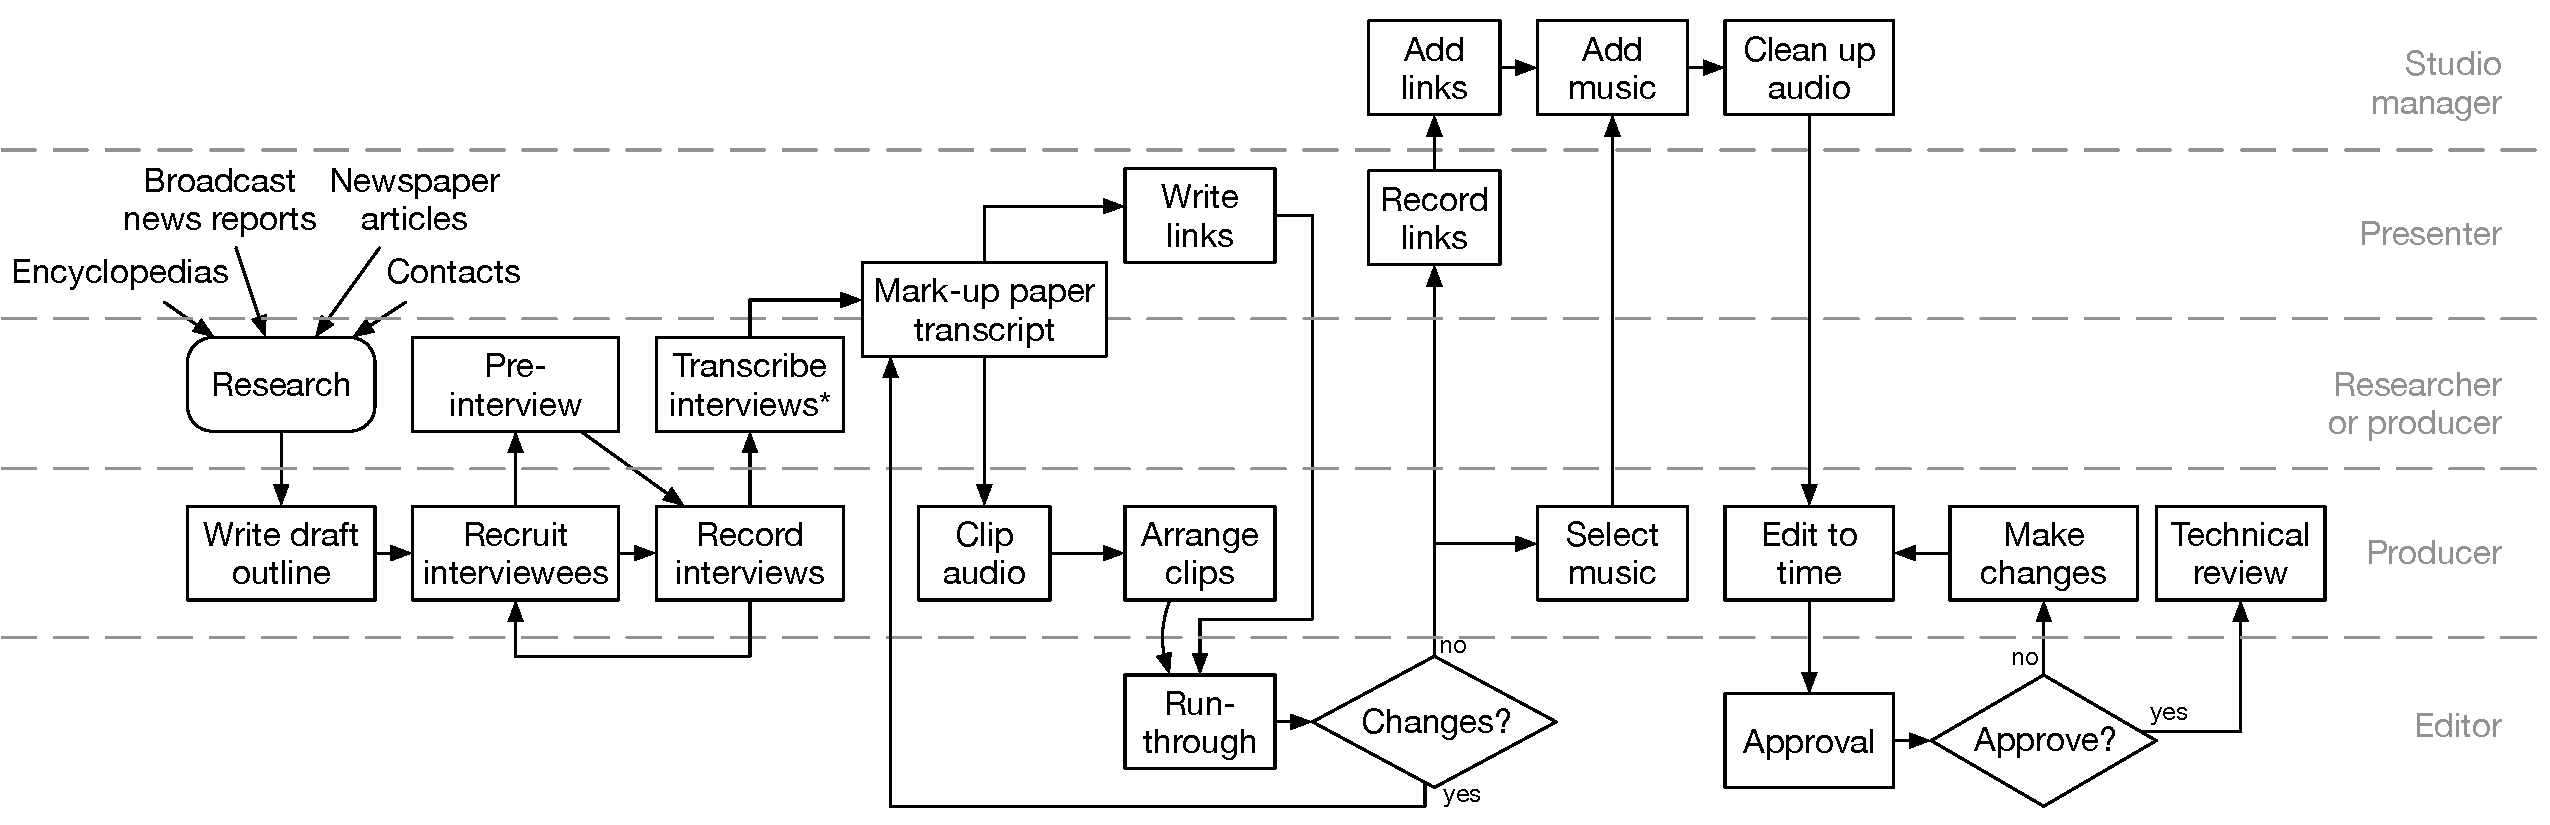
\includegraphics[width=4.5in]{figs/docs-workflow.pdf}
  \caption{Operational sequence diagram of radio documentary production, partitioned by role and location.\\
  {\footnotesize ($^{*}$some interviews are transcribed using a third-party service)}}
  \label{fig:ethno-docs-workflow}
\end{figure}

Production starts with researching the chosen topic of the documentary.  The purpose of the research stage is to form
the storyline for the documentary, and to identify people to interview.  Often the topic will be in the news that week
and the producer will be looking for an interesting angle which can be explored in greater depth.  The producer and
researcher listen to news reports and documentaries, read newspaper articles and encyclopedias, and talk to contacts
who know about the subject.  The producer makes rough notes for themselves in Microsoft Word and prepares a draft
outline of the programme.

Once the team have identified who they might want to interview, they will approach them to see if they are interested.
If the interviewee has the time available, the producer or researcher will do a `pre-interview' over the phone, which
simulates a real interview but is not recorded. This is done to see what the person will say and whether it suits the
storyline of the documentary.  Most interviews are recorded face-to-face, either on-location or in a studio, depending
on the situation.  During interviews, the presenter asks the questions while the producer records the audio and
monitors the levels.  For on-location interviews, the presenter holds the microphone and the producer operates the
portable recorder.

All of the interview recordings are transcribed. Some are recordings are sent to a third-party transcription service in
Australia that transcribes the audio overnight.  However, often the programme's budget can only cover transcription of
three or four interviews. The rest must be transcribed by the producer or researcher. For this, they use Microsoft Word
to manually type the transcript.  To save time, they will only do a rough transcription by skipping words, leaving only
enough to get a good idea of what they said.

The interview transcripts are printed onto paper, which the team use to help them collaborate.  The team go through the
interview transcripts and mark lines from they want to use with a highlighter pen. Notes and labels are informally
written on the page.  After the team have marked-up the interview transcripts, the producer uses them as a guide to
find the audio for the content they highlighted, and piece it together using a DAW into a rough edit. The transcripts
include timestamps every few minutes, which the producer can use to help them find the correct piece of audio.

While the producer creates a rough edit, the presenter writes the programme's `links' -- the narrative elements that
join the interview clips. When the first rough edit is complete, the whole team sits down with the editor for a
``run-through''. The programme is performed out loud from beginning to end, with the presenter reading the links and
the producer playing the clips from the DAW. This allows the editor to hear the programme and give early feedback. It
also allows the producer to determine the current length of the programme.  This run-through process typically happens
two or three times for each programme.

Once the editor is happy with the rough edit, a studio manager (SM) is brought it to help turn it into the final
programme.  This often happens on the day of the broadcast.  The SM records the presenter's links directly into the
DAW, while the producer sits in and gives feedback to the presenter.  The programme's theme music is added, along with
any additional music chosen by the producer. Production music is often used, which is found using an online library
such as Audio Network.  The SM cleans up the interview clips by removing redundant noises (e.g. ``umm'') and phrases
(e.g. `you know'). However, some are left in because they are difficult to remove or editorially relevant. Long pauses
are removed to ensure a good pace, but sometimes left in for effect.  The SM also balances the levels by recording
automation using a fader or by dragging in/out fades. 

Once all of the elements have come together, the producer and SM work together to cut the programme down to a specific
duration (in this case 27 minutes and 45 seconds). This is done by removing sections of speech, usually from the
beginning and end of interview clips.  The finished programme is played for the editor who gives their final feedback.
Once any changes are made and the programme is signed-off, the documentary is rendered to an audio file and imported
into the \textit{dira!} radio production system. The producer must then listen to the entire programme in
\textit{dira!} to ensure the bit-stream that will be broadcast contains no errors.

\subsubsection{Challenges and opportunities}
The documentary production relies heavily on printed transcripts, which allow the team to collaborate and make notes.
However, transcription is expensive if done using a third-party, and time-consuming if done by the team.  Transcripts
can give an idea of what was said, but it is difficult to navigate the audio to listen to a particular line.  After the
transcripts are annotated, the producer has to go back and manually edit the selected parts of the interviews, which is
a slow and tedious process.  Creating a link between the printed transcripts and the audio recordings would allow the
producers to work with transcripts as normal, but to simultaneously navigate and edit the audio content.

The editing process revealed opportunities for assisting the studio manager with cleaning-up the speech. Finding and
removing redundant noises such as ``umm''s is slow and difficult. If an acoustic model of redundant noises and phrases
could be developed, these could either be highlighted for easier identification, or removed automatically.

\section{Discussion}\label{sec:ethno-discussion}
Generally speaking, the study identified a number of opportunities to improve the handling, generation and presentation
of metadata, as discussed below.

\subsection{Text-based working}
The study found that the production teams relied strongly on scripts and transcripts of the audio content. The rough
edits for both the drama and documentary were directly created from annotated scripts of the recordings.  Additionally,
the news summaries team manually annotate their audio clips with in/out words to help them identify the recordings.
These workflows indicates that producers would much rather work with text representations than with audio on a
timeline.

Creating a link between the words in the transcript and their position in the audio could allow the producers to
navigate and edit with text as they prefer, but for the audio to be edited automatically. Hyperaudio \citep{Boas2011}
is an example of a web-based video editor that already uses this approach. In the case of dramas and documentaries, the
full text of the recordings is already available so speech alignment technology such as SailAlign
\citep{Katsamanis2011} could be used instead of full speech-to-text.

\subsection{Use of paper}
Both the drama and documentary teams preferred to work with paper copies of the scripts. Many producers are not
technology-savvy and are therefore much more comfortable with the idea of paper. It also affords them the freedom to
make unstructured notes and easily collaborate face-to-face. However, the use of paper also creates a barrier between
the work done on the page and the work done on the screen. Digital pens and interactive paper are tools that have the
potential to break that barrier while retaining the advantages of both ways of working. Further investigation is needed
to see how such a system could integrate the two approaches and whether the technology is viable.

\subsection{Redundant speech}
Observation of the fine edit in the documentary found that a significant proportion of the studio manager's time was
spent on cleaning-up interview material. Much of this was caused by redundant noises such as `umm's and `err's, or
redundant phrases like `you know'. These could be identified using a system designed or trained for the purpose.
Depending on the producer's confidence in the algorithm, it could either remove the redundant material automatically or
assist the studio manager in identifying and removing the material. 

\subsection{Speaker diarization}
All of the observed productions could benefit from being able to see where different people are speaking in a
recording, known as `speaker diarization'. In drama it would help the producers identify different lines in the script,
in documentaries it would highlight the position of the questions in interview recordings, and in news it would help
producers find what they're looking for more quickly in long off-air recordings. The research around diarization is
fairly mature \citep{AngueraMiro2012} and although it is starting to be used in some experimental BBC services such as
the World Service Archive \citep{Raimond2014}, it has yet to become available any mainstream production tools.

\subsection{Comparing takes}
Drama production is unique in the way it records multiple takes of the same content. This technique allows the
producers to get the most from the actors, but means that it can be difficult to select which performances to use.
Comparing takes during post-production is possible but the process is clumsy.  Providing an easy way to directly
compare performances would allow the director to make a better informed decision on which to use. If the rough edit for
the drama was assembled automatically, comparison could be made easier by aligning the takes on different tracks.

\section{Conclusion}\label{sec:ethno-conclusion}
An ethnographic study of radio production was conducted by exploring three case studies. It found that producers of
speech radio prefer to work with text-based representations of audio rather than with the recordings directly. Their
workflows are primarily paper-based which creates extra work when moving between paper and audio. Creating a link
between the words on the paper and their location in the audio recordings could significantly improve the production
workflow.

The study also identified opportunities to apply semantic audio technology and interaction design to radio production
tasks. Lots of time is spent cleaning up recordings by removing redundant speech, which could be fully or
semi-automated. Segmenting speech content by speaker would make a positive impact on most speech-based tasks. Finally,
drama productions could benefit from an easy way to compare multiple takes of the same scenes.


\cleardoublepage
% !TeX root = main.tex
\chapter{Screen-based semantic speech editing}\label{chp:screen}

%The producers in all three of our case studies interacted with audio content using textual representations. We also saw
%that the documentary producer wrote transcripts of all their interviews.
In Chapter~\ref{chp:ethno}, the radio producers we observed all used textual representations to navigate and edit audio
content. The drama producers used a script to write notes on what they recorded, any changes or mistakes that were made, and the
quality of the performances. The documentary producers wrote transcripts of their recordings to help them navigate and
arrange their content, and to mark up the parts they wanted to use in the programme. The news journalists also used
text to label their audio clips with the words spoken at the start and end of the clip.

In Section~\ref{sec:background-transcripts} we saw that transcripts have been successfully used to develop interfaces
that allow for semantic navigation and editing of speech content.  \citet{Whittaker2002} found that their semantic
speech interface could be used to quickly extract information and judge which parts were relevant, without having to
play the audio.  \citet{Whittaker2004} found that semantic editing was faster and as accurate as editing with a
waveform-based interface, and \citet{Sivaraman2016} found that semantic editing was more accessible than waveform
editing.  \citet{Rubin2013} presented a semantic speech interface for producing ``audio stories'', which has many
similarities to radio production. However, this system was not formally tested, so it is still unclear what effect
semantic editing interfaces have on the production of audio content.

%In Section~\ref{sec:asr}, we described how ASR can be used to automatically transcribe speech, and
% Rubin used verbatim transcript, not ASR
%Other semantic editing systems that use ASR been formally evaluated
%\citep{Whittaker2004,Yoon2014,Sivaraman2016}, but they were designed for navigating and editing voice messages and
%comments, which use a different style of audio content and have different requirements than radio production.
We saw in Chapter~\ref{chp:ethno} that the documentary producers we observed either manually transcribed their
recordings, which may not be the best use of their time, or paid a third-party to transcribe on their behalf, which is
slow and expensive.  As we discussed in Section~\ref{sec:asr}, automatic speech recognition (ASR) could be used to
replace the manual transcription process. However, the errors in ASR transcripts reduce listener comprehension
\citep{Stark2000,Vemuri2004} and increase the time it takes to search audio content \citep{Ranjan2006} and correct
errors \citep{Burke2006}. The semantic speech editor from \citet{Rubin2013} used verbatim transcripts, so it is not
clear how these errors might affect audio production. Several semantic speech editors that used ASR were formally
evaluated \citep{Whittaker2004,Yoon2014,Sivaraman2016}, but they were designed for navigating and editing voice
messages and comments, which use a different style of audio content and have different requirements than radio
production.

%We will investigate whether semantic speech editing can be used for radio production through a user study.
%To ensure the results relate to real-life requirements, we will use our access to BBC Radio to recruit professional
%radio producers, and evaluate semantic speech editing for use in production of genuine radio programmes.
%To measure its performance, we will compare semantic speech editing to the current production workflow.





%Speech is a natural form of communication which is rich in information. Since the early twentieth century, radio
%broadcasting has been used to transmit and consume speech-based content. Today, radio listenership remains high and
%podcasting continues to grow in popularity. 

%Although many radio programmes are still broadcast live, a large proportion are pre-recorded and put together using
%audio editing software. Efficient navigation and editing of speech is crucial to the radio production process.
%However, unlike text, speech must be consumed sequentially, and does not naturally support visual search techniques
%\citep{Wolfe2004}. 

%Audio editing interfaces display a visual representation of the amplitude of the sound, called a `waveform'. This gives
%users some ability to visually search and scan audio content. Although the waveform is useful for many editing tasks,
%it displays very limited information, especially when zoomed out \citep{Loviscach2011}.

%Semantic audio analysis technology can be used to extract higher-level information from the sound, such as whether it
%is speech or music \citep{Panagiotakis2005}, where different people are speaking \citep{AngueraMiro2012} or an
%approximate transcript of what they are saying.  Presenting this information to the user could allow them to navigate
%and edit audio content much more efficiently \citep{Whittaker2004}.

We were interested in investigating whether semantic speech editing can be used for radio production, and understanding
what effect semantic editing and ASR transcripts have on the production process.  In this chapter, we describe the
design and development of \textit{Dialogger} -- a semantic speech editing interface for radio production, and explain
how we evaluated our system with radio producers at the BBC.

In Section~\ref{sec:screen-requirements}, we review the existing production process to gather requirements for the
design of our system.  In Section~\ref{sec:screen-design}, we describe the design and development of Dialogger.  In
Section~\ref{sec:screen-methods}, we outline the methodology of our contextual user study in which radio producers used
Dialogger as part of the production of real radio programmes. We present the results of our study in
Section~\ref{sec:screen-results}, discuss our findings and their implications in Section~\ref{sec:screen-discussion}
and present our conclusions in Section~\ref{sec:screen-conclusion}.

% RESEARCH QUESTIONS?

%\section{Background}\label{sec:relatedwork}

%Automatic transcriptions were used by \citet{Whittaker2004}, \citet{Sivaraman2016}, \citet{Shin2016} and
%\citet{Yoon2014}, but \citet{Berthouzoz2012} and \citet{Rubin2013} chose to use perfect transcripts from a
%crowd-sourcing service.  \citet{Hyperaudio2016} used aligned subtitles and \citet{Casares2002} used a combination of
%subtitles and ASR.

%In summary, \citet{Whittaker2004} found that semantic editing of speech in voicemail is faster and as accurate as using
%waveforms.  \citet{Sivaraman2016} found that for editing discussions, semantic editing is a more accessible alternative
%to waveform editing. Systems have been developed for audio and video production
%\citep{Casares2002,Berthouzoz2012,Rubin2013,Shin2016}, but these were mostly designed without prior user requirements,
%and the studies were informal and used amateur participants. In this chapter, we describe the design of our system, which
%is based on the results of a published pilot study \citep{Baume2015}, and present our formal study, which uses real
%content and professional users in an uncontrolled working environment.

%, however most of these were
%developed without prior user requirements, none of them were tested in a formal
%user study and the informal studies that were conducted used amateur
%participants. Additionally, these In this paper we introduce Dialogger, a semantic speech editing
%system whose design is based on real-world requirements, and present the
%results of a formal user study of the system in an uncontrolled professional
%working environment.

%These studies have demonstrated the potential that transcript-based interfaces
%have for improving the navigation and editing of audio content. However, they
%have not yet been tested under real-world conditions.



%In this section, we review
%the results of the study and how it shaped the design of our system, before
%describing the features and the interface.



%We created our prototype semantic editing system `Dialogger' to assist
%specifically with the logging and rough editing stages of radio production.  Dialogger allows users to upload audio
%recordings which are then transcribed and presented in a text-based interface that allows them to navigate and edit
%the audio using the transcript.  Dialogger then allows them to export their
%edit directly into a digital audio workstation (DAW) without loss of quality,
%where they can continue with their normal production workflow.

%In order to determine how these technologies would be best applied in the
%context of radio production, we conducted a short pilot study of radio
%production at the BBC, the results of which are more fully documented in
%\citep{Baume2015}.

%, which explored the workflow, roles, motivations and
%environmental factors.

\section{System requirements}\label{sec:screen-requirements}

%The objectives of the pilot study were to discover how radio programmes are created, and to identify any opportunities
%to improve the process.  Three representative programme types were studied: a news bulletin, a drama and a documentary.
%The producers of each programme were observed and interviewed to fully document their workflow, which took between half
%a day (for news) and four days (for the documentary).

%In Chapter~\ref{chp:ethno}, we found that the participants preferred to work with text-based representations of audio,
%rather than working with the audio directly.
In this section, we will review the results of our study in Chapter~\ref{chp:ethno} and map our observations into
high-level system requirements for our semantic editing system.

We saw that the producers of the documentary ``logged'' each interview they recorded by transcribing it themselves, or
by paying a third-party service to write a full transcription.  They then used the transcripts to select which bits
they wanted to use, and copied the text to create a rough script of the programme. Once the script was mostly complete,
they had to find and cut each piece of audio for the programme, then assemble them into a draft composition known as a
``rough edit''.

Both the transcription and rough edit processes are time-consuming for the producer. Semantic speech
editing may be able to make these two production activities more efficient. We will consider these
individually to gather high-level requirements for our system.

\subsection{Transcription}
As we discovered in Chapter~\ref{chp:ethno}, radio programmes are assigned a slot in the broadcast schedule, so
producers have a strict deadline for finishing their programme. Programmes are sometimes scheduled up to three
weeks in advance, but sometimes as little as a week in advance.  This means that producers have very little time to
spare. If a programme's budget allows, interview recordings can be sent to a transcription service where they are
transcribed by a person overnight. However, many programmes do not have the budget for this, in which case the producer
transcribes the recordings themselves.

Transcripts are used to help the producer make editorial decisions, but are usually not published. For this reason, the
transcripts only have to be sufficiently accurate to use for editing. Both \citet{Whittaker2004} and
\citet{Sivaraman2016} found that the errors in the transcripts did not prevent users from being able to edit using
them. However, both also found that users wanted to be able to fix incorrect words in the transcript.

\textit{Requirement:} Our semantic editing system needs to be able to produce a transcript quickly and cheaply. It
should be accurate enough to be useful for editing, and allow for correction where necessary.

\subsection{Editing}
There are already well-established systems and software packages in place for producing radio programmes. As we discussed in
Section~\ref{sec:background-daw}, producers use a digital audio workstation (DAW) to select the parts of each interview
that they want to use in their programme, and to arrange them into a narrative. In Chapter~\ref{chp:ethno}, we learned
that the BBC provide two different DAWs --
dira! StarTrack (made by SCISYS) and SADiE (made by Prism Sound).
%Some producers prefer to use other DAWs, but as
%installation of software is restricted on corporate computers, they must use their personal computers.
Both of these use waveforms to visually represent audio to help the user navigate the recordings. The edits performed
in a DAW are ``non-destructive'' because the original recordings remain untouched (see
Section~\ref{sec:background-daw}). This allows the producer the flexibility to adjust or undo their decisions at any
point during the editing process.

For the documentary production we observed in Chapter~\ref{chp:ethno}, specialist sound engineers (known as ``studio
managers'') were brought in on the last day of production to ensure that the sound was well balanced, and to do any
advanced editing that was required. This included removal of unwanted ``umm''s or breaths in a process called
``de-umming''. The SM for the observed documentary suggested that being able to de-umm speech in a way that is
inaudible to the listener is a skilled task that requires precision, judgement and experience.

Music is often included in a programme, either as a theme tune, a short interlude or in the background. We observed
that producers
select the music either from their personal collection, or from one of a number of services for finding
commercial or rights-free music, such as Audio Network\footnote{\url{https://www.audionetwork.com/} (accessed
15.08.2016)}.  The music is added and edited using the DAW.

At the end of the editing process, the editor listens to the programme with the
producer to give their feedback and sign-off. As part of this process, they both listen out for repeated words or
phrases. However, this is only usually a problem in drama production where multiple takes of the same lines are
recorded.

\textit{Requirement:} Our semantic editing system needs to be able to select and arrange parts of audio recordings.
Given that there are well-established radio production systems for advanced editing tasks such as de-umming and
addition of music, it also needs to be able to integrate with these so that it can be used in professional radio
production.

% - Select parts of recordings and arrange into order
% - 

% Transcription X Need transcripts quickly X Not much money for transcripts X Transcripts aren't published, need to be
% good enough (Whittaker2004)
% X Whittaker says that correction would be good
%
% Integration
% X Existing system in place for broadcasting
% X Currently use waveforms
% X Must be non-descructive
%
% Web-based
% X New software can't be installed
%
% Drag and drop
% X Production involves picking bits out of interviews
% X Sorting, trying out different orders
%
% Umms/breaths
% X De-umming is skilled and done in DAW
%
% Music editing
% X Music discovery is done using existing systems
% X Editing is done in DAW
%
% Repeats
% X Repeats don't happen in interviews, only in drama really

\section{System design}\label{sec:screen-design}
This section describes the design of our system, as guided by the requirements set out in
Section~\ref{sec:screen-requirements}. We explain our choice of transcription, editing interface and excluded features
before describing the functionality and operation of Dialogger.

\subsection{Transcript}
We considered three factors when choosing a transcription method -- turnaround time, cost and accuracy. Manual
transcriptions are nearly 100\% accurate, however they are expensive (about \$1 per minute) and slow (typically 24
hours). Automatic transcriptions are imperfect, but cheap (about \$1 per hour) and fast (quicker than real-time
listening). Our system requires quick and cheap transcripts that are sufficiently accurate, so we chose to use automatic
transcripts generated by a state-of-the-art commercial web service\footnote{\url{https://www.speechmatics.com/}
  (accessed 15.08.2016)}.
\citet{Whittaker2004} and \citet{Sivaraman2016} found that users want to be able to correct the transcript, so we
designed our system so that users can fix incorrect words.
\citet{Rubin2013} did not include this feature as they used verbatim transcripts.

\subsubsection{Speaker diarization}
%The speech-to-text system we chose to produce transcripts generates additional information from the audio. It attempts
%to identify the people speaking in the recording by their gender and a numeric identifier (e.g. [M2], [F5]). Also, for
%each word, the system assigns a value between 0 and 1 of how confident it is that the word is correct. We decided to
%include these extra pieces of information, as they should both be useful to the producer.

As part of the transcription process, the ASR system performed speaker diarization (see
Section~\ref{sec:background-diarization}), gave each speaker an identification number and estimated their gender.  We
segmented the transcript into paragraphs to indicate changes in speaker, and used a text label at the beginning of each
paragraph to display the gender and identification number (e.g.  [M2], [F5]).  \citet{Rubin2013} also identified
speakers by placing their respective parts of the transcript in different columns.  However, this approach limits the
number of speakers by the number of columns that can be displayed. By labelling paragraphs, we are able to support
multiple speakers.

\subsubsection{Confidence shading}
The ASR system provided us with a rating for each transcribed word that indicated the system's confidence in the
accuracy of that word.  As we discussed in Section~\ref{sec:background-confidence}, \textit{confidence shading} is a
technique used to shade words that fall below a confidence threshold.  \citet{Suhm2001} found that confidence shading
slowed down correction, but \citet{Vemuri2004} found that it improved comprehension. However, neither of these results
were statistically significant.  \citet{Burke2006} did not test the performance of confidence shading, but the study
participants reported that confidence shading was helpful for identifying mistakes in the SCANMail interface.  On
balance, we chose to include confidence shading because the findings from \citet{Vemuri2004} and \citet{Burke2006} are
based on more modern ASR systems.

%The speech-to-text system can recognise esoteric words like `ribosome' and `ARPANET', but can struggle with
%colloquialisms and casual conversation. If the recording is too quiet or noisy, or a word isn't in its dictionary, the
%system makes a best guess (e.g. `subbuteo' was translated as `some beauty'). It also

%Recorded interviews have at least two people speaking (sometimes more), so it
%is helpful to know where in the recording they are speaking. Our system attempts to detect where there is a change of
%speaker, then inserts a new paragraph for each speaker with a unique label including their gender (e.g. M2, F5).  We
%selected this layout over Rubin's approach of having separate columns
%for each speaker so as to allow more than two speakers.

\subsection{Interface}

Our semantic editing system needs to be able to select and arrange parts of audio recordings. To achieve this, we used
the same drag-and-drop interface as \citet{Hyperaudio2016} as it is a simple method for extracting and re-ordering
clips. It also allows clips from different recordings to be added and re-arranged. \citet{Casares2002},
\citet{Sivaraman2016} and \citet{Berthouzoz2012} used a select/delete interface, where parts of an individual
transcript can be chosen or removed, and \citet{Whittaker2004} and \citet{Rubin2013} used a cut/paste/delete interface.

We designed our interface to be browser-based, as the BBC corporate policy meant that it was not possible to install
new software on the producers' computers. This came with the added benefit of allowing users to work from anywhere in
the world on any operating system, but the downside that they have to be connected to the Internet.

\subsection{DAW integration}

Our system needs to be able to integrate with the existing radio production tools. We designed Dialogger to be used as
the first stage of the editing process, and to smoothly integrate with the DAWs that are used in BBC Radio. We achieved
this by providing a novel features to export edited content from our system, either as a .wav audio file or as an ``edit
decision list'' (EDL).

The first option exported a single .wav audio file of the edit. This method is a ``destructive'' edit, in that it
throws away the pieces of the recording which weren't selected.  The other option exported an EDL, which contains
metadata about which parts of an audio or video recording make up an edit. These can be read by the two most common
audio editors used at the BBC -- SADiE and dira! StarTrack.  This method is considered ``non-destructive'' as the full
original recordings are retained and the edit points can be re-adjusted in the audio editor.
%Following early informal feedback, features were added to allow the text to be printed or exported into a word
%processor.

\subsection{Excluded features}

%\citet{Rubin2013} and \citet{Berthouzoz2012} included detection and removal of `umm's or
%breaths as this was generated as part of the crowd-sourcing service.  We did not include this functionality as we found
%during the pilot study that removal of `umm's and breaths is a highly specialised task that cannot yet be
%automated to a professional standard.  Additionally, as our system is based on
%speech-to-text, information about the position of `umm's and breaths is not
%available.

\citet{Rubin2013} included features for finding music tracks and creating loops within them.  In
Chapter~\ref{chp:ethno}, we found that specialist tools are already used for finding and choosing music, and that
editing of music is already efficiently handled by the DAW. Therefore, we chose not to include features for adding or
editing music. 

\citet{Rubin2013} also included detection of repeated words and phrases. We chose not to include this, as we found in
Chapter~\ref{chp:ethno} that repeats are only an issue in drama production. As the production of drama involves a very
different workflow of recording multiple takes of lines from a script, we chose to focus on production workflows for
pre-recorded content in our system design or study.

%\begin{figure}
%\centering
  %\includegraphics[width=\columnwidth]{figs/transcribetime.pdf}
  %\caption{Time taken to transcribe each recording with linear trend line}
  %\label{fig:transcribetime}
%\end{figure}

\subsection{System description}

This section gives a brief overview of Dialogger, including its functionality and operation.  A screenshot of the
interface and numbered list of the main features are shown in Figure~\ref{fig:interface}.
%A live demo of the system is
%also available\footnote{\url{https://speecheditor.virt.ch.bbc.co.uk/demo} (accessed 15.08.2016)}.

\begin{figure*}[ht]
\centering
  \includegraphics[width=\columnwidth]{figs/interface-labels.pdf}
  \caption{Screenshot of the user interface with highlighted features: (1)
    individual user accounts and projects, (2) upload of audio recordings, (3)
    list of uploaded recordings, (4) waveform display of currently selected
    recording, (5) toolbar with playback, save, copy and print functionality,
    (6) transcript of selected recording with speaker labelling and word
    editing, (7) confidence shading, (8) transcript selection with
    drag-and-drop editing, (9) listing and re-ordering of edits, (10) duration
    of edit, (11) export edit to audio file or digital audio workstation.}
  \label{fig:interface}
\end{figure*}

\subsubsection{Transcript}\label{sec:transcript}

The ASR system we chose was evaluated using a large multi-genre television dataset \citep{Bell2015}.  It had an overall
word error rate of 47\%, however for news content, which is clearly spoken by a native speaker, this dropped to 16\%.
As the speech on radio programmes is similar in nature to speech on television news, we found the error rate to be
comparable. However recordings with non-native speakers or significant background noise had a higher error rate.  For
comparison, the reported error rate of the system used by \citet{Whittaker2004} was 28\%, and for \citet{Sivaraman2016}
it was 10\%.

The time taken by the transcription service to process each uploaded recording was approximately half as long as the
length of the recording. The time depends primarily on the length of the recording but also on noise, accents and the
complexity of the speech.

%\subsubsection{Functionality}
%Dialogger is web-based speech editing tool that can be accessed from anywhere
%using a web browser.
%Users can upload their own speech recordings into a project in their individual user
%account. Each recording is automatically transcribed at around twice
%real-time speed, with a word error rate of approximately 16\%.

%The interface displays a list of the user's recordings on the left, the transcript of the selected recording in the
%middle, and a blank workspace on the
%right. The waveform of the selected recording is also shown at the top.
%Users can play a recording, and navigate it using either the transcript or the waveform.

%The transcript is divided into paragraphs at points where the speaker changes. Each paragraph is labelled with the
%speaker's assigned identity, including their gender (e.g. [M3]). Words that might not be correct are shaded grey, and
%incorrect words can be fixed by the user. Buttons at the top of the transcript
%allow the user to print the transcript, or copy it into a word processor.

%Recordings can be edited by highlighting and dragging words from the
%transcript to the workspace on the right, which creates a clip. Multiple clips
%can be created and re-ordered to produce an edited version. The edited version
%can be played to allows users to preview the result. The user can save their
%edit to revisit later.

%The interface displays the total duration of the edit. The edited version can
%be exported as either a .wav audio file, or as an edit decision list (EDL) for
%a digital audio workstation (DAW).

%TODO Add block diagram?
\subsubsection{Operation}

The functionality and operation of the system is described below as a typical user journey. Each feature is numbered
and shown in Figure~\ref{fig:interface}.

Users access Dialogger by navigating to a web page in their browser. They start by logging into the system using their
account (1) and create a project where they can upload their speech recordings (2) that appear in a list on the left
(3). Each recording is automatically transcribed. When it is opened, the waveform appears at the top and the transcript
appears in the middle section.  The recording can be played (5) and navigated by using the waveform (4) or by clicking
on a word in the transcript (6). The transcript shows where different people are speaking using paragraphs labelled
with the speaker's gender and an identification number (e.g. [F2]). Words which are likely to be incorrect are shaded
grey (7), known as `confidence shading'.  Incorrect words can be fixed by double-clicking them and typing the correct
word.  The transcript text can be copied or printed using buttons at the top. The audio can be edited by selecting a
range of words (8), then using drag-and-drop to place it in the area to the right which creates a clip (9).  Clips can
be re-ordered and deleted. The total duration of the edited clips is displayed (10). The edited audio can be played
through to preview the result, and the edit can be saved. Finally, the edited clips can be exported as a .wav audio
file or as an EDL (11) for further editing in a DAW.

%During this period there was no easy
%way to listen to the audio, so although they know \textit{what} was said, they
%don't know \textit{how} it was said.

%After editing using the transcript, the producer must go back to find and cut
%each piece of audio they wanted to use in the programme, known as a `rough edit'. Moving from audio to text and back
%again is costly, but is considered by the producers to be worthwhile. We believe that by linking audio and text
%representations together in a single editing system, it would be possible to
%work with either representation without incurring the cost of converting between the two.

%The pilot study also found that some of the functionality included in previous
%studies is already efficiently handled, or cannot yet be automated. For
%example, advanced music discovery platforms like Audio
%Network\footnote{\url{https://www.audionetwork.com/}} allow producers to
%quickly find music tracks of the right length, and removing `umm's or breaths
%from speech transparently is a skilled task that requires fine editing and
%human judgment.

 %It found that producers of speech radio prefer to work with
%text-based representations of audio rather than with the recordings directly.
%Their workflows are primarily paper-based which creates extra work when moving
%between paper and audio. Creating a link between the words on the paper and
%their location in the audio recordings could significantly improve the
%production workflow.

%The study also identified opportunities to apply semantic audio technology
%and interaction design to radio production tasks. Lots of time is spent
%cleaning up recordings by removing redundant speech, which could be fully or
%semi-automated. Segmenting speech content by speaker would make a positive
%impact on most speech-based tasks. Finally, drama productions could benefit
%from an easy way to compare multiple takes of the same scenes.

%\subsection{Design}
%We designed Dialoger to play to the strengths of transcript-based editing by
%focusing on the key features for logging and rough editing, and integrating
%well with the current production workflow. We excluded some features like
%removing `umm's or adding music, which are better handled by existing systems or techniques.  We also excluded
%detection and handling of repeated phrases, as this technique is only used in drama production.

%This section describes the design, features and implementation of the prototype.




%\subsubsection{Transcription} \subsubsection{Layout}
%The interface is laid out so that the workflow operates from left to right.
%Recordings are uploaded and listed on the left (2), the transcript of the
%currently selected recording is shown in the middle (6), and clips are created and exported on the right (9). The
%waveform of the currently selected recording is shown at the top on a dual time-line (4), where the bottom waveform
%shows the entire recording and the top is a magnified display of the current position.

%\subsubsection{Navigation} Users can navigate the selected recording by clicking on a word in the
%transcript, which seeks to that position and starts playback, or by clicking on
%the waveform to jump to a specific time. Playback can also be controlled using
%buttons in the toolbar above the transcript (5).

%The text before and after the current playback position is coloured black and
%dark grey, respectively, to indicate the current playback position in the
%transcript.  Words which the speech recognition system is not confident about
%are shaded in light grey (7), known as `confidence shading'.


%\subsubsection{Editing}
%An audio clip can be created from the transcript using drag-and-drop.  The user
%selects text from the transcript (8) then drags and drops the selection in the
%space to the right.  Each clip is contained in a shaded box (9) which can be
%re-ordered by dragging them up and down, or deleted by clicking an `X' in the
%top right of the box.

%The clips can be played using the playback buttons at the top, or by clicking
%on a word. The total length of the clips is displayed above the text (10).


%\subsection{Implementation}
%The system was implemented using web standards, which allowed a consistent
%experience on any recent web browser, and avoided the need to install any
%software locally. The front-end was written in Javascript using the Hyperaudio
%\citep{Hyperaudio} and peaks.js \citep{Peaks} libraries, and the back-end was
%built using Node.js and MongoDB running on a virtualised Ubuntu server.
%Communication between the two was done through a REST API.

\section{Evaluation methodology}\label{sec:screen-methods}

We wanted to determine whether professional radio producers could successfully employ the features of Dialogger as part
of the production of a real radio programme. Specifically, we were interested in measuring whether semantic speech
editing was faster than their existing technique, and if it continued to be used after the trial.  We also wanted to
investigate how the semantic editor was used and whether there were any features that could be added to improve the
functionality.

Additionally, we wanted to take this opportunity to continue our research on the existing radio production workflow to
learn more about the challenges producers face and the tools they use to produce their programmes. Our study in
Chapter~\ref{chp:ethno} did not explore requirements in-depth, and there is not much previous literature that analyses
actual radio production practice, so we wanted to be able to inform researchers and designers about real requirements
and behaviour in this field.

To achieve these goals, we conducted a qualitative contextual study of radio producers working under two conditions --
the existing editing workflow and the semantic editing workflow.

%\subsection{Research questions}
%The questions we aim to answer through this study are as follows:
%\begin{itemize}
  %\item What is the workflow used by radio producers to create a pre-produced radio programme?
  %\item What challenges do radio producers face in creating a pre-produced programme?
  %\item Which tools do radio producers currently use for editing audio, and how are they used?
  %\item Can a semantic editing system be used in the radio production workflow?
  %\item Do radio producers edit audio faster using a semantic editing system compared to their existing system?
  %\item When left with access to a semantic editing system, do radio producers continue to use it?
%\end{itemize}

\subsection{Approach}
Gaining access to radio producers can be difficult as there are not many of them and they are normally very busy.
%A number of unrelated studies on television production systems have previously been conducted
%\citep{Engstroem2010,Perry2009}, but 
%We were only able to find two studies which used radio producers.
For example, \citet{Kim2003} attempted to recruit radio producers but was unsuccessful because the producers were ``so
highly tasked''. However, in this case we were able to recruit professional radio producers from the BBC Radio due to
the access available to us from working within the BBC.

%To account for this, we designed our study to take place at their desk and to overlap as much as possible
%with the work they already need to do.
As we would not be able to recruit a large number of participants, we chose to take a qualitative approach to maximise
the depth of the information gathering. To take advantage of the available access to the work environment, we chose to
use contextual inquiry techniques to allow us to learn about the workflows, tools, and the social, technical and
physical environments. This took the form of an initial interview, followed by a period of observation, then a final
interview.

Radio producers find it difficult to step away from their day-to-day work for too long.  To account for this, we
designed our study so that the tasks overlapped with
the production of the programme that the participant was working on at the time, and the audio
content they needed to edit that day. We interviewed and observed participants in their normal working environment to
ensure that the production workflow was not affected by an artificial setting.

\subsection{Recruitment}

We invited professional radio producers with at least five years of experience to take part by sending an email to
departments in BBC Radio that create pre-produced factual programmes.  Drama programmes were excluded from the study as
we saw in Chapter~\ref{chp:ethno} that their production workflow involves making multiple recordings of lines in a
script and selecting the best ones. This is a sufficiently different process to other programme genres that it warrants
a different interface.

Five participants (P1--P5) were recruited (4 male, 1 female) who each had between 6 and 20 years experience in working
as a radio producer. Although we had a small number of participants, the experience of the producers and the depth of
the study means that their feedback should carry significant weight. Five participants is also considered sufficient
for identifying most usability problems \citep{Nielsen1993}.

During the experiment, the participants worked on programmes of different
lengths from a range of genres:
P1 produced a single 27-min documentary, %plus 50-min for WS
P2 produced a 27-min documentary as part of a ten-part series,
P3 produced a single 45-min documentary,
P4 produced a 14-min archive programme
(based around material from the archive) as part of a ten-part series, and
P5 produced a single 27-min magazine show (covering multiple stories on a
single theme).

\subsection{Procedure}
We designed a five-stage experimental procedure that followed a typical contextual inquiry format of
interview/observation/interview. In addition, we recorded some simple metrics such as task completion time and feature
usage.

\paragraph{Stage 1: Background interview}
    The participants was first given an overview of the project and the study, and asked to complete a consent form. This
    was immediately followed by a semi-structured interview to learn about the participant's background, their existing
    production workflow and the tools they used. The investigator asked the participant to describe the
    radio production process in detail, and used follow-up questions to clarify their understanding. This information
    was recorded using written notes.

\paragraph{Stage 2: Dialogger training}
    %A short training session on the Dialogger interface.
    Each participant was trained on the functionality of the Dialogger interface using a pre-written ``tool-tip tour'',
    in which the participant was presented with a sequence of instructional pop-up dialog boxes overlaid on the
    interface.  This ensured consistency of training between participants. Each participant was then issued with a
    series of tasks that utilised all of the system functionality. The investigator observed this stage and wrote notes
    of any unexpected behaviour or stumbling blocks.

\paragraph{Stage 3: Task observation}
    %Observing the participant as they produced a radio programme.
    Each programme is composed of a number of interviews
    on a single topic, or set of topics.  We observed the participant while they logged and rough-edited two
    different interviews for the same programme. They did this by editing an interview under each condition -- one
    using their existing production workflow, and the other using Dialogger. The order of the conditions was
    counterbalanced.

    The investigator sat beside the participant during the task and wrote notes on the workflow, tools, generated
    metadata, usability issues, task completion time, and unexpected reactions or usage.
    The actions of the participant on Dialogger were logged electronically. After they completed the task, they were
    asked to rate each condition using the NASA Task Load Index metrics \citep{Hart1988}.

    %The tasks were performed as part of the production of a real radio programme,
    %and the observation was done in the participant's normal work environment.

\paragraph{Stage 4: Interview}
    We conducted a semi-structured interview about the participant's experience of each system and how they compared.
    The investigator questioned participants about the advantages and disadvantages of each workflow, then asked about
    any specific topics, issues or questions that cropped up during observation. The audio from this interview was
    recorded and transcribed to allow for further detailed analysis.
    %The questions asked were:

    %\begin{itemize}
        %\setlength\itemsep{0em}
      %\item Which aspects of the existing system did you / did you not find useful?
      %\item Which aspects of the prototype system did you / did you not find useful?
      %\item Overall, which system did you prefer and why?
      %%\item Did the prototype change the way you made the programme? If so, how?
    %\end{itemize}

\paragraph{Stage 5: Longitudinal deployment}
    Each participant was then given access to Dialogger for a further month, and was invited to continue to use it if
    they wished. Each week, they were asked via email whether they had been using the system, and if so, which features
    they valued most/least or were missing.  During this time, their usage of Dialogger was also logged electronically.

\subsection{Analysis}
Our study produced observation notes, interview transcripts and metrics. We used thematic analysis with open, flat
coding to interpret the textual data, and we used statistical analysis to process the numerical data, as described below.

\subsubsection{Coding}
We manually transcribed the audio recorded from the interviews in Stage 4 to produce a verbatim transcript, and
collated them with notes made by the investigator from Stages 1, 2 and 3. To organise and process this textual
information, we employed the use of thematic coding techniques.

We performed a two-stage coding process.  Firstly, we openly coded each part of the transcripts using grounded theory
\citep{Silverman2016} into a flat structure.  As there are not many previous studies on radio production, we decided to
use open coding so that the categories would emerge from the data we collected, rather than attempting to test an
existing model.  We used the software package RQDA \citep{RQDA} to execute this stage.

Once all of the text had been processed, we grouped the codes that had common themes. We used mind-mapping software to
help us re-arrange the codes into various hierarchical structures until a logical solution was found.  The coding
and grouping was performed by the investigator that collected the data.

\subsubsection{Metrics}
Although this was primarily a qualitative study, we chose to collect some basic metrics to measure task completion
time, cognitive load and usage after the trial.

We used task completion time from Stage 3 as a metric for editing speed. As participants used different interviews of
varying lengths for each condition, we measured task completion time relative to the length of the audio
recording being edited. We used a paired \textit{t}-test \citep[p.~17]{Shalabh2009} to test for any significant
difference between the existing and semantic editing workflows.

To measure the cognitive load of each task, we used the raw TLX metrics gathered from the questionnaire in Stage 3. We
used a paired \textit{t}-test on each of the six metrics to test them individually for any significant differences.

Finally, to measure the level of usage during the longitudinal deployment in Stage 5, we collected the time spent using the
interface, the number of new uploads and the number of exported edits. As this data is only relevant to the semantic
editing workflow, we will report the raw numbers.

\section{Results}\label{sec:screen-results}

The coding process resulted in 40 codes, which were grouped into ten categories and four themes (see
Table~\ref{tab:codes}). The codes contain comments about both the existing and semantic editing workflows, however for
clarity we will present these results individually.

We start by going through the existing radio production workflow in detail, with an emphasis on the challenges that
were identified, and the tools that are used as part of the process. We then consider the semantic editing workflow and
expand on the four themes identified during coding. Finally, we look at the results of the metrics that we captured
during the observation and longitudinal deployment.

\begin{table}[h]
\centering
{\small
\begin{tabular}{|p{0.18\linewidth}|p{0.2\linewidth}|p{0.5\linewidth}|}
\hline
\textbf{Theme} & \textbf{Category} & \textbf{Codes} \\ \hline
\hline
\multirow{5}{*}{Comprehension}
 & Challenges & Complexity, quantity, environment, concentration, time taken \\ \cline{2-3}
 & Navigation & Speed, search, paragraphs, speaker segmentation, time since recording, cross-referencing \\ \cline{2-3} 
 & Accuracy & Correction, accents, good enough, confidence shading, use after editing \\ \hline 
\multirow{3}{*}{Organisation}
 & Mark-up & Bold, star rating, labelling, annotation, timestamps, word processing \\ \cline{2-3} 
 & Programme script & Structuring, collaborating with presenter \\ \hline 
\multirow{2}{*}{Editing}
 & Sound quality & Fast playback, anxiety of not listening \\ \cline{2-3}
 & Technique & Deleting, workflow, transcript not needed for short edits, similarity to TV \\ \hline
\multirow{3}{*}{Usability}
 & Portability & Laptop, paper \\ \cline{2-3} 
 & Drag'n'drop & Space on clipboard, scrolling \\ \cline{2-3} 
 & Misc & DAW integration, transcript turnaround time, simultaneous uploads, video support, waveform, avoidance of repetition \\ \hline
\end{tabular}
}
\caption{Topics, categories and codes that emerged from analysis of the interviews in Stage 4 and the
observation notes from Stages 1, 2 and 3.}
\label{tab:codes}
\end{table}

\subsection{Existing workflow}\label{sec:resultsexisting}
%\subsubsection{Observation}
%During the first interview, participants worked with the investigator to
%identify a particular task in their workflow that would form the basis of the
%observation. In every case, logging and rough editing of an interview was
%selected, as this process takes a long time, is considered tedious and would
%benefit from automatic transcription.

%Due to the pressured and changing work environment, the observation had to fit
%around the editing requirements at the time of observation. This meant that P4
%and P5 did not do any logging during observation.

This section describes the existing radio production workflow. The process is documented as described by participants
in the interviews (Stages 1 and 4) and as witnessed by the investigator during the observation (Stage 3).  We start by
describing the production workflow, then we discuss the topics identified through thematic coding.

\subsubsection{Workflow description}

This section describes the high-level production workflow for pre-produced content as described by the
participants. This is also represented by the numbered diagram in Figure~\ref{fig:workflow}, and the description below
uses numbers to make reference to each part of the diagram.

\begin{figure}[ht]
\centering
  \includegraphics[width=.6\columnwidth]{figs/workflow.png}
  \caption{Radio production workflow as described by participants}
  \label{fig:workflow}
\end{figure}

When a programme is commissioned, the producer starts by researching the
subject (1) in detail to identify a compelling story and to find the best
contributors. This is done by reading, listening and watching existing material
on the subject, and finding and talking to relevant people. During this time
they also recruit a presenter for the programme.

After researching the topic, the producers then arrange interviews with
contributors and record them (2) with the presenter either in a studio, an external
venue or via a telecommunication link.

% Quote from P3
%Once you've got all the interviews recorded, before you start formally scripting and cutting the programme, you log
%them. You don't transcribe them precisely, but you do a rough transcription that is sufficient to copy those bits of
%text in to script, sufficient to find the bits of the audio you want to use and to make sense to the presenter.

Once material has been recorded, the next step is for the producer to select which parts of the audio they want to use
in the programme.  This selection process is often aided by creating ``logs'' of the interviews.  Logging (3) helps the
producer by allowing them to see, on screen or on paper, what was said in each interview, when and by whom, without
having to listen to it.  This allows them to quickly find and share the pieces that they want to use in the final
programme.  It also helps them structure their thoughts, identify themes running through discussions, and make links
between different interviews.

\begin{figure}[ht]
\centering
  \includegraphics[width=\columnwidth]{figs/phil-desk.jpg}
  \caption{P3 logging interviews with a digital audio workstation on the desktop
    PC and word processor on the laptop}
  \label{fig:desk}
\end{figure}

Logs are usually written by the producer themselves. As they have done the research and are normally present at the
recordings, they can use their memory to navigate the material and use their experience to quickly determine which
parts are relevant. As we saw in Chapter~\ref{chp:ethno}, some programmes that are under particular time pressure will
use a third-party to create a verbatim transcript of a few interviews, but most do not because it is too expensive.

In the observation, P1 and P3 wrote their logs in Microsoft Word whilst using a digital audio workstation (DAW) to play
the recording (see Figure~\ref{fig:desk}). P5 reported that they usually followed a similar process, but did not do any
logging during observation.

The exact format of the logs varied between individuals, but they usually contained a rough transcript of the interview
with occasional timestamps and notes. They reported that this helped them to find important bits in the recording later
on. Each producer has their own syntax, but there are commonalities.

Timestamps were written on the logs, approximately \textit{``every 30 to 120 seconds''} (P1) with minutes and seconds
in parenthesis: \texttt{(4'20)}, for example.  This allows the producer to navigate to a particular piece of audio much
faster than they would otherwise by narrowing down their search range.

The next stage is to rough edit (4) each recording, which involves segmenting the audio into chunks, removing the
chunks they don't intend on using, and to label and arrange the remaining chunks.  The editing reduces the amount of
material they need to work with, and the labels make it easier to identify which parts are which.  If a recording is
short (around 15 mins or less), then this process is usually done without logging the content first.

This process of recording, logging and rough-editing is repeated until the producer has enough material for their
programme. Throughout this process, a script is used to organise and structure (5) the content of the programme.  The
script usually takes the form of a Microsoft Word document, but can also be written on paper. Some producers only write
a rough outline, whilst others will copy in full transcriptions of the content they are using.  Some producers have an
idea of what the programme will look like before they make any recordings, so will create the script first. Others will
be guided by the content of the interviews, so will wait until they have some recordings before creating a script.

\textit{``As I'm organising a programme, booking interviews, talking to contributors, and planning interviews, I'm all
the time assembling a scratch structure that will eventually be the script.''} (P3)
% It's not set in stone unless it has to be

The script is also used to collaborate with and get feedback (6) from the presenter.  Using a written document rather
than audio files makes it easier to quickly review the content of the programme, make notes and suggestions, and to do
this over large geographic distances. The presenter uses the document to write and insert ``links'', which are the
narrative elements spoken by the presenter to link the interview clips into a story. They also insert comments and
notes for the producer. Once the script is nearing its final stages, the presenter records (7) their links and sends
them to the producer.

If the programme is part of a series, it will often have theme music. Any other music is chosen (8) by the producer,
often using production music services such as Audio Network\footnote{\url{http://audionetwork.com} (accessed 28/4/17)},
or the BBC's Desktop Jukebox.

Once the interview, links and music are ready, the producer will assemble these into an edit (9) that matches the
script, using the DAW. This edit will be about twice as long as the final programme, sometimes significantly longer
(e.g. P5 reported that they once created 22-hour-long rough edit for a 37-min programme). The producer then continues
to edit the audio, primarily to ``get it down to time'', but also to give it a final polish by cleaning up the audio.
Cleaning involves finely adjusting sound levels to be consistent, removing ``umm''s and breaths, and adding non-speech
sounds to create a rich auditory scene.  Producers who are skilled at using a DAW will usually clean up the audio
themselves, but others will bring in a sound engineer (known in the BBC as a ``studio manager''), to help with this (10).

Before a programme is broadcast, it must be signed-off by the department head, known as the ``editor''. Most producers
will get feedback from the editor (11) before this, so that they have time to make any requested changes. Often this
happens a day or two before transmission. Some participants reported that they sit in the room with the editor while
the current version is played, while others sent an audio file to the editor to listen by themselves. In both cases,
the editor gives oral feedback and suggests changes.  Once the editing is complete, a final version is rendered to an
audio file and added to the playout system for the editor to sign-off (12).

% Quote from P3
%So once you've got that done, you then start using your structure to assemble sound, assemble scripts, write links to
%go with those bits of transcript in the structure as it becomes a script. 

% Quote from P3
%The way I do it is that I have a piece of paper with the names of the sections, the rough amount of time I'm budgeting
%for each one and once I've done an assemblage of the amount of time I've got of each one I can see I've got 37 mins for
%part one where actually I need 4 mins and that motivates you to crunch it down. You just keep going round and round and
%round that until you get something that's coherent, clear and to time.

%\paragraph{(7) Record presenter} The next stage is to add narrative elements, known as `links' to join the clips
%together into a storyline. The producers reported that they work with their presenter to write the links together,
%using the programme script to collaborate. The presenter records the links in a studio and the producer then assembles
%them into the edit.

We now consider the comments made by participants, organised by the categories from the thematic coding (see Table~\ref{tab:codes}).

\subsubsection{Challenges of comprehension}

The skill of the producer is to \textit{``separate the wheat from the chaff''} (P1, P3, P4 -- all verbatim) and to find
the clips which will make an interesting programme.

\textit{``That's the basis of my job - to find great stuff and put it together.
  It's not difficult putting it together, it's finding the great stuff and finding connections between it. Getting rid
  of the non-great stuff is
  challenging and time-consuming, and it requires mental processing.''} (P1)

However, the sheer quantity of recordings means this process adds significant overhead.

\textit{``you've got an average of 45 mins per interview and in a series of
  three programmes you've got seven per programme, that's a lot of work''} (P3)

Interviews recorded for speech radio often cover complex topics in fine
detail. Keeping track of all the points raised and forming a compelling
narrative from them is a challenge.

\textit{``All the interviews overlap with each other terribly, and have got
  similar themes.''} (P4)

Writing the logs takes a lot of concentration as the producer must listen to
what is being said, work out how it ties in with other contributions and the
story, and make swift judgements on whether it should be used.

\textit{``one of the slightly exhausting things about doing it is the level of
  concentration you have to maintain to make good decisions, remember where
  everything is, what you've got, is kind of strained rather by having to just
  do schleppy tasks like moving the sound and logging interviews''} (P3)

P1 and P5 reported that they find the office environment distracting, so often work at home or outside the office.

\textit{``I typically do this at home because I find it a much less distracting
  environment. It does require quite intensive concentration so you don't miss
  something.''} (P1)

%Quote from P5
%Where I find it useful is when I'm away from the office and away from the machine, and that sort of thinking time
\textit{``In the office there's so much pressure and you're always doing stuff.''} (P5)

Although P4 did not do any logging during observation, they explained that for longer recordings, they
would normally write logs by hand in a notebook whilst listening on a
portable music player somewhere away from the desk, such as in a caf\'e.

The high level of concentration required, combined with the repetition of 
typing and listening to the interview again means that producers need to take
regular breaks.

\textit{``it's boring and it's not very easy to be efficient at it [...] when
  I'm normally doing it I'm checking my emails, making a cup of tea.''} (P3)

\subsubsection{Programme script}
The producers organised the programme by writing a ``script''. This is primarily used to help them structure their
thoughts, but also to help communicate with the presenter over email.

%The scripts contain varying amounts
%of detail, depending on the subject and the individual producer. Some will
%eventually include a full transcription of the programme, whilst others will
%remain as a bullet-point outline.  The scripts are written using Word, with P2
%also using `MindManager' mind mapping software.
%The script can be created at any point during production, but is often started
%during the research stage.
In the study, P1, P2 and P5 started their scripts during the research stage by writing an ordered list of bullet points
of topics to cover and a list of draft questions to ask contributors.  P3 and P4 waited until after they had done some
interviews to start the script, as they wanted to structure the programme around the discussions that they recorded.

P3 and P5 updated the script after every edit to ensure they were always in sync. This added significant overhead but
gave them a visual structure to follow when making the final changes.
Having an accurate script also makes it easier to re-use the programme afterwards, when creating another version of a
different length, or for pulling out clips for the website.

%\textit{``What was really good was being able to take the final script that I had typed up as I was editing and tie it
  %to the finished programme in the system.
\textit{``[The script] is going to be invaluable when it comes to re-cutting this.''} (P5)

\subsubsection{Mark-up}

P1, P3 and P5 would make comments for themselves in the log to help them when
editing. For example, ``\textit{[good to here, dull after]}'' or
``\textit{[trails off 9'30]}''. P1 also used a star rating system to rate the
quality of each point, for example ``\textit{[**** should use this stuff, but
  dramatically cut down]}''.

\textit{``What I sometimes do when I edit are star good bits, and I think
  that's quite a common trait.''} (P3)

Bold highlighting was also used by P1 and P3 to mark bits of the transcript
which are important and worth keeping.

\textit{``what I did was just put in bold the paragraphs I thought were worth
  [keeping]''} (P1)

P2 used a different approach to logging their material. Instead of logging the material by writing a transcript, they
played the recording in a DAW and used a keyboard shortcut to create timed markers at any points of interest. By seeing
where the markers clustered, they identified where to make clips, then gave each of the clips labels. This approach
allowed them to focus more on the audio, but didn't allow them to make any detailed notes.

\subsubsection{Sound quality}\label{sec:existing-quality}

Radio is an audio-only medium, so the quality of the content is highly dependent on the quality of the sound.  The
criteria producers use for deciding whether a piece of audio is good enough to use in their programme is not just about
what was said, but how it was said and how well it was said.

\textit{``How people say things is very important.''} (P5)

On the one hand, producers need to listen out for any poor quality sound that might negatively affect the programme,
such as people mumbling, stumbling, coughing, or any excessive background noise. 

\textit{``I've done paper edits before where I've gone back to that bit of audio and they didn't quite finish the
  sentence or they muttered it. You just couldn't use it at that point.''} (P3)

However, the producers were are also listening out for anything that worked particularly well, such as a moment of
comedy or passion, or a sound that perfectly captures the right feeling. Identifying these using the text of a
transcript is very difficult or impossible. 

Every participant that performed logging played the audio faster than real time at least once. This allowed them to
efficiently listen out for anything they might want to use while reviewing parts of the interview that may not be of
interest (e.g. off-topic or ``off-mic'' discussions).  P2 also used faster playback to prevent themselves from
over-thinking their edit decisions and picking out too much material.

\textit{``The ability to listen at faster than real-time [...] gives me the opportunity to come to a swifter decision.''}
(P2)

%\textit{``There's quite a lot of judgement I've got to make just on what the listening quality is.''} (P2)

\subsubsection{Edit technique}

If the recording was short and had been recorded recently, as was the case for P4 and P5, it can be edited
without first creating a log.

\textit{``If it's a quick ten minutes with three questions, you don't need to bother''} (P3, also P4 and P5)

In this situation, we observed that the producers listened through the recording using a
DAW and pressed a keyboard shortcut to split the recording, usually at the beginning/end of questions/answers. They
then went back to remove unwanted segments and add labels to the remaining ones.

In the cases where the recording was logged (P1, P2, P3), the producers used the log to decide which parts to select or
remove. They used the timestamps written in the log to narrow down their search area for each clip they extracted.
However, even with a reduced search area, the producers found it time-consuming to find the exact start and end point
of each clip using the DAW interface.

In the study, three of the participants (P3, P4 and P5) used SADiE as their DAW, which is provided to the producers by
the BBC. However, the other two participants chose to use other software packages that aren't formally supported. P1
used Adobe Audition because they were familiar with the interface and it was installed on their laptop, unlike SADiE
which was only available to them on a desktop computer.

P2 comes from a television production background and used Apple's Final Cut Pro, which is primarily a video editor but
also includes audio editing functionality.  P2 used Final Cut Pro because they were familiar with the interface and had
it on their laptop. In addition, they enjoyed being able to import audio directly from video content without having to
use another program to extract the audio first, and being able to use the video ``titles'' feature to make written notes
that can later be viewed in time with the audio.

\subsection{Semantic editing workflow}\label{sec:resultsnew}
This section discusses the results and themes that emerged from the evaluation of the semantic editing interface.
Participants were first introduced to Dialogger through a training stage (Stage 2). All of the
participants completed the training without any major issues. However, this stage highlighted a requirement for
keyboard shortcuts which was not previously identified.  P2 and P3 kept trying to use the space bar to start and pause
audio playback. This is a common shortcut in most DAWs which these participants naturally reached for. Reports on
previous semantic editing systems have not mentioned keyboard shortcuts, however they could be used to assist the
editing process.

In the rest of this section, we will discuss each of the themes that came out of the thematic coding (see Table~\ref{tab:codes}).

%To evaluate the semantic editing interface, participants were observed while
%they used the system to log and rough edit recordings for a programme.
%Although it was designed as an all-in-one solution for putting together a rough
%edit for a programme, participants used the interface in different ways to
%integrate with their existing workflow.

%P3, P4 and P5 used the interface much as designed by using the transcript
%window to read and identify suitable clips, then dragging them across to the
%edit window and exporting the audio.


%P1 completed the test quickly and without issue,
%expressing that it was easy and intuitive. The other four participants
%successfully completed the test, but identified a number of minor usability
%problems regarding keyboard shortcuts.

%Two of the five participants (P2 and P3) kept pressing the space bar to start and pause audio playback. This may be
%habitual, as it is a universal keyboard shortcut in all DAWs. However, this feature was not considered when designing
%Dialogger.  Additionally, P2 tried to use word processing shortcuts in the
%interface, such as Ctrl+C and Ctrl+V to copy/paste and backspace to delete.

%P1, P2 and P4 reached for Ctrl+F to search for a word they were looking for. Although this feature wasn't explicitly
%implemented or mentioned in the training, the functionality was included in the browser. The participants remarked
%that it was a powerful tool for navigating the recording.

%In conclusion, we found that keyboard shortcuts are more important than we had
%considered when designing Dialogger.

%The interface was designed to allow users to copy the text of the entire
%transcript by pressing a `copy' button. Four of the five participants
%intuitively selected the text before pressing the copy button.  P2 expressed a
%preference to use Ctrl+C and Ctrl+V shortcuts to copy and paste text, rather
%than a drag-and-drop gesture.  Additionally, P2 said they wanted to be able to
%remove selected text by pressing backspace, or to export only selected text.
%Future versions should
%consider allowing users to apply actions only to selected text.

%Three of the five participants (P2, P3 and P5) couldn't remember the action to
%correct a word (double-click). Two of them (P2 and P3) right-clicked the text
%and looked for an option in the context menu.

%P2 confused about double waveform

%\section{New workflow}
%Following the usability study, participants were observed using the prototype
%interface to complete a common production task and interviewed about it
%afterwards. This section documents the findings.

\subsubsection{Navigation}

Participants reported that having the transcript available in the semantic
editing interface allowed them to read and search the recordings much faster
than they normally would with a waveform, which is in line with previous findings from
\citet{Whittaker2004} and \citet{Yoon2014}.

\textit{``with having a transcript you're able to immediately scan through it
  10/15 times faster. Maybe that's an exaggeration but it feels ten times
  faster''} (P1)

The transcripts also allowed the participants to quickly cross reference what
was said in various interviews without having to listen through multiple times.

\textit{``where I'm picking shorter clips, making a point and moving on or I'm
  developing an argument between different people and cutting between them, it
  feels a lot more easy to construct that `on paper' than what I'm currently
  doing''} (P2)

%\textit{``If it's a shorter thing I'll bang it straight into SADiE and start
  %editing down to find the wheat from the chaff''} (P4)

Being able to click on a word to navigate to that point in the audio also
enabled the participants to use visual search to quickly find and listen to
bits they were looking for.

\textit{``you can do that with your eyes even quicker - zone straight in on the bits and that click to go  `that bit',
  `that sentence there', `that word there' ''} (P4)

Participants reported that editing with a transcript was primarily useful when working at the sentence level. When the
granularity of editing involves removing individual words, ``umm''s or breaths, they said that the DAW software is much
better suited to these tasks. This supports our design decision to integrate with DAWs.

\textit{``the real editing work actually happens after this has passed its main
  point of usefulness''} (P3)

%\textit{``I was using some interviews, some contributors recorded on one
  %ocassion, but across several programmes, several episodes in a series, or for
  %several different stories.''} (P4)

%\subsection{Navigation speed}

%\textit{``it took me 15 mins to read 35 mins and not just read, but read and mark
  %up''} (P2)

%\subsection{Time since interview}

%\textit{``you're kind of doing a paper edit on the basis of having recently
  %heard the audio''} (P3)

%\textit{``a lot of that guesswork was coming from the memory of being there at the recording... realising which bits
%were the questions from the presenter and which bits were answers.''} (P2)

%\textit{``I know I've got a doc coming up in six months time, so I'll ask them
  %some questions for that. Now then in six months time I can't remember what
  %the answer was''} (P4)

%The primary benefit of reading over listening is that you can quickly scan ahead and jump around with your eyes,
%whereas listening can only be done at a fixed pace. 

\subsubsection{Transcript accuracy}
When using the semantic editing interface, editing decisions are based on an
automated transcript which is only partially accurate. Previous research has shown that for editing
voicemail recordings \citep{Whittaker2004}, discussions \citep{Sivaraman2016} and spoken comments \citep{Yoon2014},
automated transcripts were considered sufficiently accurate. However, the ASR transcript accuracy required for
navigation and editing in radio production is currently unknown.

The participants in our study suggested that the transcripts were, generally speaking, sufficiently accurate for their
purposes.

\textit{``It's clearly not 100\% in word recognition but I'm feeling it's
  certainly good enough for my rough cut purposes at this point''} (P2)

If the recording being edited was made recently, the producer can use their
memory of what was said to make sense of the inaccuracies in the
transcript.

\textit{``Both these interviews [being edited] are relatively recent so I have
  it reasonably in my mind what they've been saying. I was able to read roughly
  what there was - `okay that's that question', `I know what was in that
  question' ''} (P1)

In the existing radio production process, transcripts are used to aid the producer and presenter, but are
  not shared outside of the production team. In our study, the producers we observed only used the transcript
  to navigate and edit the audio. However, P3 and P4 noted that they were interested in correcting the transcript later
  so it could be shared or published.

\textit{``I'm probably posting transcripts for the whole interview. So I do
  need to go through and correct''} (P4)

Being able to provide corrected transcripts has the potential to make an impact beyond improving the
  editing workflow. For example, transcripts of the finished programme could make the audio content searchable and
  re-usable for print media.

%Clearly, the more accurate the words in the transcript are, the less work has
%to be done to correct it.

%\textit{``The closer it can be to the point where you don't have to clean it up
  %the better obviously, and that's quite significant honestly, that's my only
  %qualm''} (P3)

%Sometimes a word is commonly mistranslated throughout the transcript, so
%providing an easy way to fix that would be a useful addition.

%\textit{``Something that would be even better is Ctrl+H  replace function''} (P3)


%\section{Speaker diarization} One disadvantage of working with transcripts is that you can't hear which person is
%speaking when.

%\textit{``if you can't see who's speaking - that's a disadvantage''} (P3)

%Speaker diarization technology \citep{AngueraMiro2012} can be used to try and
%identify where different people are talking. The prototype included a
%rudimentary system that attempted to distinguish speakers and guess their
%gender, however it tended to significantly overestimate the number of speakers
%which caused some difficulty. 

%\textit{``It was distracting if anything, partly because I was trying to guess
  %who was which at certain points''} (P2)

%However, in many situations the participant could tell who was who from what
%they were saying.

%\textit{``It's reasonably clear to me who's asking the questions, but actually
  %[speaker diarization] is helpful''} (P1)

%During the study it was discovered that many producers record in stereo and use
%the waveform to see where people are speaking.

%\textit{``I always pan the presenter on one side and the contributor on the
  %other so I can see where the questions are''} (P5)

%This workaround could be exploited to improve the performance of a more
%advanced speaker diarization system.

\subsubsection{Mark-up}
%Before creating any clips, P1 immediately copied the transcript text into Word
%in order to allow them to make annotations.

%The WAVs were then imported into the DAW
%by dragging and dropping them from the file system.

%In the observation stage, it was identified that annotation is an important
%part of the production process that was missing from the prototype.

During the study, P1 and P3 copied the transcript text from the interface into Microsoft Word. They
reported that they did this because there was no annotation functionality
available within Dialogger.

They inserted paragraph breaks, added notes after paragraphs, and
highlighted desired parts of the transcript in bold. Once the transcript was
annotated in Microsoft Word, they went back to Dialogger, found the parts of the
transcript they wanted by scrolling though the text, then dragged and
exported each clip individually as a .wav file.

\textit{``it would be better to take raw lumps of transcripts and plonking them
  in Word because Word has higher functionality than this''} (P3)

Producers are very familiar with the Microsoft Word interface so a later version of our
system could seek to provide a similar interface. This would allow producers to make annotations in the same way they
do already.

\textit{``With text editing, the reflexes are very much Microsoft Word''} (P4)

The most basic feature that could be added is highlighting, which is often used to note parts of interest

\textit{``If you just put a little star or underline or something simple to
  mark things, that would be a big gain for a small change''} (P3)

%\textit{``sufficient to find the bits of the audio you want to use and to make
  %sense to the presenter.''} (P3)

%\subsection{Star rating}

%\textit{`` I just gave myself a detailed breakdown of what was said in the
  %interview with timecodes at questions or major new points and a slightly
  %arbitrary scoring system to say 'that's really good stuff and must get in'.
  %''} (P1)

\begin{figure}[t]
\centering
  \includegraphics[width=\columnwidth]{figs/highlighting-cropped.jpg}
  \caption{P2 using a highlighter pen with a printout}
  \label{fig:highlight}
\end{figure}

\subsubsection{Portability}

P5 reported that working on paper allowed them to be productive outside of
the office, such as during their commute.

\textit{``What would be really useful would be to [...] take it away (say when
  I'm on the train going home) and I would paper edit the bits that I need''}
(P5)

Additionally, working on paper allows them to work anywhere as it does not
require electricity.

\textit{``It's highly portable. It doesn't require any power.''} (P2)

In the observed task, after uploading their recording, P2 immediately printed
the transcript and read through it on paper so that they could work away from
the screen.

\textit{``I'm reading a lot of material for a sustained period so I'd prefer to do it on page than on screen. Just
  easier on my eyes.''} (P2)

% Quote from P5
%you want to get away from the screen at some point

P2 then used a highlighter pen to select the desired parts of the recordings (see Figure~\ref{fig:highlight}).  After
highlighting all the pieces they wanted,
they then used the Ctrl+F text search to find the highlighted words in Dialogger.

\textit{``it allowed me to get to clips very quickly from a reference point on a printed transcript''} (P2)

However P2 noted that having timestamps on the printout may be a faster
way of achieving the same thing.
Once they had found and clipped all of the highlighted parts in Dialogger, they exported the clips into SADiE.

P4 explained that for an upcoming programme, they were
planning to print out transcripts from Dialogger to help
them collaborate with their presenter.

\textit{``we're just going to go through it with a pencil and paper, with a
  printout, and highlight the bits we want and cross out the bits we don't.''}
(P4)

\subsubsection{Sound quality}
Part of the appeal of having a transcript is that it frees the user from listening to the audio in real-time. It also
allows users to work on paper, away from any electronic devices. However, disconnecting the audio from the text
fundamentally changes the production process.

\textit{``Radio is made with your ears. You'll never get away from that fact that you need to listen''} (P4, also P2,
P3, P5)

There was also concern that parts which sounded great but didn't come across as well in the transcript may have been
overlooked.

\textit{``I was anxious it might not have sounded as good as it read, or that I might be missing bits that sounded
  great ''} (P2)

As discussed in Section~\ref{sec:existing-quality}, the participants existing workflow includes playing the audio
faster than real time, but that feature was not included in Dialogger.  Several of the participants noted that they
would like to have this feature added.

\textit{``it's a little bit annoying that there's no facility for that.''} (P2)

Although faster than real time playback normally reduces intelligibility, this may be less of a problem if the
transcript was available.

\textit{``you do still need to listen through, even though you've got the text.  Therefore, it would be optimised if we
  could listen through quickly''} (P4)

As listening is an important part of the production process, semantic audio interfaces would benefit from providing
easy access to the underlying audio to allow multi-modal interaction. Once the link between the audio and the text is
broken, re-linking the two together can be costly.

%\textit{``It's not very good at spotting breaths. You're always going to need [a DAW] for the fine edit.''} (P4)

%\textit{``Actually listening through to what sounds best, what is better audio, more entertaining inflexion of speech
  %rather than what is the content of those words. Those sorts of things you obviously can't tell from the written
  %page''} (P4)

\subsubsection{Drag-and-drop}

In Dialogger, we used a drag-and-drop technique for users to create clips from various interviews and
re-order them in a clipboard area. All of the participants were able to use this successfully, however we quickly
encountered issues when dealing with longer clips.

\textit{``I found the interface quite clunky for pulling out big chunks of audio''} (P5)

We performed our initial testing by pulling short clips, but for real-life usage, participants were mainly interested
in creating large clips. This quickly filled up the clipboard area and users struggled to find the space to add more
clips. This finding is in contrast to \citet{Sivaraman2016} which found that participants were mainly interested in
making small edits.

P2 suggested modifying the interface so that clips were created by selecting the text and using a button to add the
clip to the end of the clipboard. The problem could also be addressed by collapsing and expanding the clips to minimise
the area they occupy.

%Difficult to highlight long text as it is off the screen, have to scroll down.
%P1 and P4 suggested using shift-click with cursor.

\subsubsection{Usability}

Users could transfer their edits from Dialogger to a DAW by saving and opening a file. However, some
participants wanted much tighter integration with the DAW, including bi-directional transfer of edits, so that edits
made in the DAW were reflected in the semantic editor and vice-versa.

\textit{``Instead of thinking about it as a paper edit, if you think of it as the paper edit result of the sound
  edit''} (P3)

None of the participants found the waveform display in Dialogger to be useful, and found it to be an
unnecessary addition to the transcript text.

\textit{``You're either working with text or working with the waveform. You don't need both.''} (P5)

Some participants also noted that they would prefer a cut-and-paste approach to copy-and-paste, as this prevents any
duplication of content. This could also be achieved by marking which parts of recordings have already been used.

\textit{``When you have a big load of stuff, it's comforting to know that you're not duplicating your work.''} (P4)

%\subsubsection{Interface design}
%The semantic editing interface was designed so that the user could drag and
%drop selected clips into an edit window. Although this works well for picking
%out short clips, user encountered issues when trying to select and use long
%clips as the edit window quickly filled up.

%\textit{``I found the interface quite clunky for pulling out big chunks of
  %audio.''} (P5)

%Users worked around the problem by dropping new clips between old ones, then
%re-ordering the new clip to the bottom of the list. One suggested fix was to
%have a button to append a clip of the selected text to the edit without having
%to drag and drop.

%\textit{``once you've selected on the left hand side [...] it would go to the
  %bottom of the queue, that would be a useful way of moving stuff from left to
  %right for pulling highlight clips''} (P2)

%Selecting very large amounts of text with a dragging motion also proved tricky,
%so it was suggested that clicking whilst holding shift (like in word
%processing) could fix this.

%\textit{``Just being able to hold shift and use the cursor. Selecting the text
  %was a little bit index finger intensive.''} (P4)

%Although the semantic editor is set up to select good bits, a lot of the
%participants also wanted to get rid of bad bits.

%\textit{``What you need to do is [...] to get rid of the gubbins of me talking
  %to presenters and mistranslating''} (P3)

%Some were also interested in having cut functionality that would remove the
%selected clip from the original recording. This would ensure that it can't be
%used twice.

%\textit{``You could even go further in the spirit of what it is which would
  %being able to cut and paste, delete''} (P4)

%Not all of the participants agreed though.
%\textit{``it wouldn't be something I'd be aching to be introduced''} (P1)

%\subsubsection{Stage of usefulness}

%\textit{``The transcript is useful at a later stage in the production process
  %when I've cut my programmes, when I want to export clips to the news. When I
  %need to compile a final script for a presenter''} (P2)


%\subsubsection{Quantity}

%\textit{``We've got about six hours of audio for a one hour programme, and it's
  %all just one-on-one interviews''} (P4)

%\textit{``you've got to find the right bit which is burdonsome and annoying
  %when you've got 20 interviews to do''} (P1)

%\subsection{Export}

%Stuff on export and integration

%No gaps in WAV

%\subsection{Export}
%Each participant differed in how they exported the
%content.

%P5 made a list of all the clips they wanted for the programme before exporting
%them into SADiE.  P4 made clips for three different programmes from a set
%of eight recordings. They did this by making a list of clips for one programme
%then exported them into SADiE before moving onto the next programme.

%P3 took a different approach by exporting each clip individually as a .wav file
%which they renamed.  Additionally, P3 copied the text from each clip into the
%script for their programme. They then inserted paragraph breaks between
%questions and answers, and highlighted the questions in bold so that they could
%easily identify them.

%P4 queried whether it would be possible to identify which parts of the
%recordings had already been used, so that they wouldn't be re-used in other
%programmes.

%\subsection{TV}

%Two participants suggested that text-based editing would be equally, if not
%more, useful for TV production. P2, who formerly worked in television, said
%that their workflow already followed a similar pattern. 

%\textit{``If I was making a TV show this is what I would do. I'd effectively
  %print [a transcript], read, highlight, pull a collated collection of those
  %clips or number then, then write a draft script that combined everyone's
  %interview highlight clips that I thought were relevent for telling the
  %story.''} (P2)

%The costs involved in producting TV content are much higher than radio, so
%there is a greater financial incentive in streamlining the process.

%\textit{``There's an advantage to paper edit in TV because the assemblage
  %process takes longer and you might decide you don't need particular bits of
  %archive you thought you did and [save on] transfer costs.''} (P3)

% ran out of space

%\subsubsection{Longitudinal deployment}\label{sec:followup}


\subsection{Metrics}\label{sec:resultsmetrics}
\subsubsection{Time}

\begin{figure}
\centering
  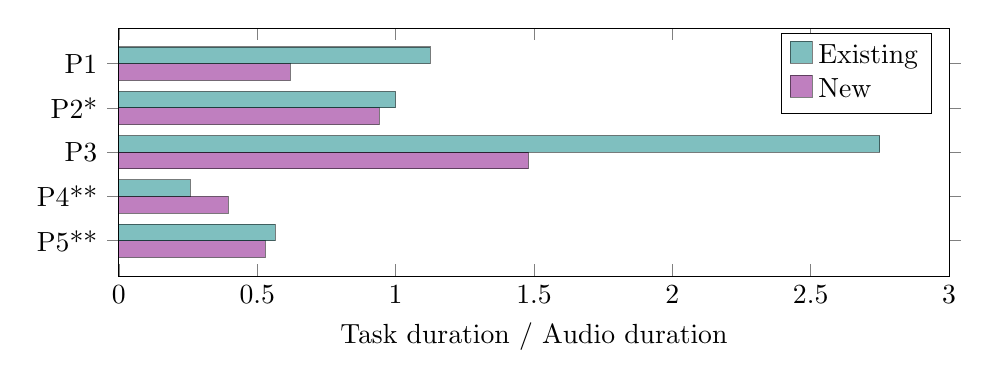
\begin{tikzpicture}
  \begin{axis}[
      width=\columnwidth,
      xbar=0pt,
      bar width=6pt,
      xlabel=Task duration / Audio duration,
      y=16pt,
      xmin=0,
      xmax=3,
      enlarge y limits=0.2,
      symbolic y coords={P1,P2*,P3,P4**,P5**},
      ytick = data,
      y dir=reverse,
      reverse legend,
      legend cell align={left},
      ]
  \addplot[fill=violet, opacity=0.5] coordinates {(0.619,P1) (0.941,P2*) (1.48,P3) (0.395,P4**) (0.529,P5**)};
  \addlegendentry{New}
  \addplot[fill=teal, opacity=0.5] coordinates {(1.125,P1) (1.0,P2*) (2.75,P3) (0.258,P4**)
    (0.565,P5**)};
  \addlegendentry{Existing}
  \end{axis}
  \end{tikzpicture}
  \caption{Time taken to complete the observed task for each workflow, compared to the original audio length. Lower is
    better. *P2 logged their material on paper. **P4 and P5 did not do any logging. Due to the small sample size and
    variation in usage, no conclusions about time performance can be drawn.}
  \label{fig:time} \end{figure}

We recorded the time participants took to complete the observed tasks (see Figure~\ref{fig:time}). As various
recordings of different lengths were used for the existing and new workflows, we divided the edit time by the audio
duration to calculate the relative edit time.  In all cases, the producers were able to run the ASR processing as a
background task so this was not included in the calculation. P1, P2 and P3 used the semantic editor after their
existing process, while P4 and P5 did the opposite. However as different recordings were edited on each system, the
presentation order is not expected to affect the results.

The mean average time for semantic editing was 0.79 minutes per minute of audio, versus 1.13 minutes for the existing
method, which is a 44\% improvement. However, a paired \textit{t}-test revealed that there was no statistically
significant difference (\textit{p} = 0.24).  This is due to the small sample size and the large variations in timings
resulting from P4 and P5 not doing any logging, and P2 printing out and annotating their transcript before editing.
Semantic speech editing may have the potential to reduce the time needed for logging and rough-editing material, but
further investigation with a larger sample and consistent workflow is required to measure time performance.

%P2 did go through a logging stage, but did this by printing out the generated transcript and using a highlighter pen
%to select the bits they wanted. This meant that they had to go back and repeat this process using the semantic editor
%interface, which slowed them down. Despite this, the new process was marginally faster.

%P1 and P3 used Dialogger as designed by logging and editing their material using the semantic editing interface. The
%length of their interviews were also much longer, so the benefit of text-based navigation and editing was more
%apparent. In this case, the producers rough edited their material 85\% faster compared to their existing workflow.


\subsubsection{Cognitive load}


%\begin{table}
  %\centering
  %\begin{tabular}{ r | c c c c c | c } & P1 & P2 & P3 & P4 & P5 & Mean \\
    %\hline
    %Mental demand   & -5  & -9  & -2  & 5   & 4 & -1.4 \\ Physical demand & 0   & 4   & 0   & 13  & 0 & 3.4 \\
    %Temporal demand & -1  & 4   & -5  & 4   & 1 & 0.6 \\ Performance     & -2  & 7   & 0   & 2   & 5 & 2.4 \\
    %Effort          & -1  & -7  & 7   & -4  & 2 & -0.6 \\
    %Frustration     & -12 & 1   & -3  & 2   & 5 & -1.4 \\ \hline \end{tabular}
  %\caption{Difference in NASA-TLX results between the old and new workflows.
    %Negative results indicate that the new workflow is better.} \label{tab:tlx} \end{table}

After completing both tasks in the observation, the participants were asked to
rate both the old and new workflows using the raw NASA-TLX metrics
\citep{Hart1988}.
%The results are shown in Figure~\ref{fig:tlx}.
No significant differences were detected for any of the metrics using the paired \textit{t}-test.
With only five participants and marginal differences, it was not possible to
draw any conclusions about cognitive load from these results.  They indicate
that Dialogger requires slightly less effort and mental demand, and is less
frustrating.
However it is considered more physically demanding, temporally
demanding and scores lower in performance.

%To put these results in context, we must look at what the
%participants said in the interviews.

%\begin{figure}
%\centering
  %\begin{tikzpicture}
  %\begin{axis}[
      %width=0.8\columnwidth,
      %height=0.8\columnwidth,
      %bar width=6pt,
      %xbar=0pt,
      %xlabel=Mean TLX value,
      %y=16pt,
      %xmin=0,
      %xmax=100,
      %enlarge y limits=0.15,
      %symbolic y coords={Frustration,Effort,Performance,Temporal demand,Physical demand,Mental demand},
      %ytick=data,
      %legend pos=east,
      %legend style={at={(1,0.5)},anchor=east},
      %reverse legend,
      %]
  %\addplot[fill=violet, opacity=0.5] coordinates {(44.5,Frustration) (53,Effort) (41,Performance) (51.5,Temporal demand) (48,Physical demand) (51,Mental demand)};
  %\addlegendentry{New}
  %\addplot[fill=teal, opacity=0.5] coordinates {(48,Frustration) (54.5,Effort) (35,Performance) (50,Temporal demand) (39.5,Physical demand) (54.5,Mental demand)};
  %\addlegendentry{Old}
  %\end{axis}
  %\end{tikzpicture}
  %\caption{Mean NASA-TLX results for each system. Lower is better.}
  %\label{fig:tlx}
%\end{figure}

\subsection{Longitudinal deployment}

After the interviews and observations were complete, the participants were given access to Dialogger for a further
month (Stage 5). During this time their actions were logged electronically and they were emailed each week to ask which
features they found useful, or were missing. P3 was unavailable immediately after the study, so could not take part in
this stage.

Most of the comments received in the longitudinal deployment were already picked up by the first part of the study. In
the remaining comments, all of the participants said they enjoyed being able to use Dialogger outside of the office and
at home. Some reported that they had issues uploading content with their slow network connections, and P2 suggested
that allowing multiple simultaneous uploads would allow them to leave it running overnight.

Participants were given access to the system for one month after the study.  The logs from the interface were analysed
to see how the participants used Dialogger during this stage of the study.
All of the participants continued to use the semantic editor of their own accord as part of their work. The total time
spent by the four remaining participants (P1, P2, P4, P5) using Dialogger in the month-long deployment period was 23
hours and 58 minutes.  Over 14 hours of those were from P2, with P4 using it for 5 hours, P1 for 3 hours and P5 for 20
minutes.  During this period, 86 recordings were uploaded and 58 audio edits were exported.

%\begin{figure}
%\centering
  %\begin{tikzpicture}
  %\begin{axis}[
      %width=0.8\columnwidth,
      %%height=0.7\columnwidth,
      %bar width=6pt,
      %xbar=2pt,
      %xlabel=User actions,
      %y=11pt,
      %xmin=0,
      %xmax=320,
      %symbolic y coords={Printed edit,Copied edit,Printed transcript,Deleted clip,Copied transcript,Exported audio,Uploaded audio,Re-ordered clip,Created clip},
      %ytick=data,
      %nodes near coords,
      %]
  %\addplot[fill=teal, opacity=0.5] coordinates {(3,Printed edit) (5,Copied edit) (12,Printed
    %transcript) (12,Deleted clip) (22,Copied transcript)
    %(58,Exported audio) (86,Uploaded audio) (178,Re-ordered clip) (270,Created clip)};
  %\end{axis}
  %\end{tikzpicture}
  %\caption{Count of logged user actions during follow-up}
  %\label{fig:actions}
%\end{figure}

Users could navigate the content by either clicking on the waveform or by clicking on a word in the transcript. The
interaction log showed that over 98\% of navigation actions were executed by clicking on a word, which shows a clear
preference for navigating by text compared to waveforms.

%\section{Implications}

%Remove as well as take away

%Annotation is import. Need to include word processing features

%Paper is still used, portable and easy on eyes

\section{Discussion}\label{sec:screen-discussion}
%Two key aims of radio production are to find the most relevant or interesting parts of speech recordings, and
%assemble them into a story.
We found that producers face a number of challenges with audio editing in radio production. There is often a large
quantity of audio to process so it can take a long time. The content of the speech is usually complex and contains
interconnections to things said in other recordings, which can be difficult to keep track of. Making editorial
decisions also requires a high degree of concentration over an extended period, which is demanding, especially in the
noisy and distracting office environment.

We observed that in their existing workflow, participants tackled these challenges by employing a number of techniques
to filter and arrange their audio content. They started by listening back to all of their recordings, which allowed
them to simultaneously assess the editorial content and sound quality of the audio. For long recordings, many
participants ``logged'' the audio as they listened, by typing rough transcriptions and notes into a word processor, which
they later used to help them edit the audio using a digital audio workstation (DAW). For short recordings, instead of
logging, participants segmented their recordings in the audio editor during playback, and went back to remove unwanted
segments and label the rest.
%Double-speed playback was often used to skim through some of the audio.
All of the participants used a word processor to create a programme script in which they developed the structure and
content of their story. They used annotations to highlight or rate the transcripts, and wrote notes to help them with
selecting and assembling the final content.

We introduced a semantic editing system into professional radio production, which the study participants were able to
successfully use as part of their workflow. On average, the semantic editing workflow was much faster than the existing
workflow, in line with previous findings from \citet{Whittaker2004}, but this result was not statistically significant,
so requires further investigation.  We compared the semantic editing workflow, which included a transcript, to the
existing workflow, which did not. Therefore, we were unable to measure how much benefit was derived from the transcript
itself, compared to the semantic editing interface.  All participants voluntarily continued to use the system after the
trial, which indicates that they found value in using it. However, we identified a number of important features that
were missing or could be used to improve future semantic speech editing systems. These related to listening,
annotation, collaboration and portability.

\subsubsection{Listening}

Logging is an important process that primarily involves labelling and organising content, however it is time consuming.
%Natural language processing could also be used to assist this process. For example, a text segmentation algorithm
%\citep{Choi2000} could divide an interview into different topics, and a keyword extraction algorithm \citep{Matsuo2004}
%could provide a summary of what was discussed. However,
Some participants found the logging process to be valuable
because it gave them the opportunity to listen back through their recordings, and make connections between various bits
of content. This cross-referencing could also be assisted by providing links between words within and between
recordings. For example, selecting a word could display and replay other mentions of that word in other recordings.

Another important reason for listening is to ensure a high ``sound quality''. Participants wanted to avoid low quality
audio such as ``umm''s, mumbling, coughing and excessive background noise, but they also wanted to ensure they didn't
miss any high quality audio moments that might not have been identified using the transcript.  Faster playback is
already used in radio production to reduce the time spent listening to material, however more sophisticated time
compression algorithms such as those described by \citet{Arons1997} could be used. Time compression has not been
included in previous semantic editing systems, but should be considered in the future, especially as \citet{Vemuri2004}
found that the maximum time compression factor is significantly higher when an automated transcript is present.

Removal of ``umm''s and breaths, known in radio production as ``de-umming'', is either done by the producer themselves or
with the help of a sound engineer, depending on the producer's experience and time pressure. To maintain sound quality,
the removal of umms/breaths must be audibly transparent and participants reported that this can difficult to achieve.
Previous semantic editing systems have included functionality to remove umms \citep{Berthouzoz2012} and breaths
\citep{Rubin2013}, however these were made possible because the manually generated transcripts 
explicitly transcribed those items. ASR systems are normally trained to ignore umms/breaths rather than
transcribe them, which prevented us from including this functionality. A transcription system that includes these would
allow us to add this functionality, however further research is needed into the extent to which de-umming can be
automated in this way.

\subsubsection{Annotation}

All of the participants used a script document to structure and assemble their programme, and as a
medium to inform and gather feedback from the presenter about the content and layout of the programme. Although the
clipboard of our semantic editing system acted much like a programme script, the participants did not use it in that
way because it was missing some key functionality for annotation and collaboration.

Annotation features were an important requirement that we did not pick up on during the design specification, and which
have not been included in previous semantic speech editing systems. Two participants in our study deviated from the
expected workflow in order to annotate the transcript, and the other participants noted the absence of such
functionality. Participants wanted to be able to annotate the transcripts as they would with a word processor, in order
to highlight or rate particularly good parts of their recordings, add personal comments, and to segment and label the
content.

A simple change to achieving this would be to allow the transcripts to be formatted, and for textual comments to be
inserted and edited. Furthermore, the drag-and-drop editing could be replaced with cut/copy/paste similar to
\citet{Whittaker2004} and \citet{Rubin2013}. An alternative approach could be to add semantic speech editing
functionality to a word processor, rather than adding word processing functionality to a semantic speech editor.

\subsubsection{Collaboration}

Scripts are used as a tool for collaborating with colleagues such as the
presenter because the programme's content and structure can be quickly reviewed and
commented on by others without them having to spend time downloading and listening to the audio. Our semantic editing
system was designed for individual access to transcripts and edits, however this meant that they could not be shared
with the presenter. A better approach would be to allow multiple users to navigate and edit the same material. This
could be achieved using operational transformation \citep{Sun2004} which can support concurrent users editing the same
content. Participants were also interested in tighter integration with the DAW. The same technology could be used
to create bi-directional integration with DAWs, so that any edits made in the DAW are automatically updated in the
semantic editor and vice-versa.
%Collaborative annotation features such as those explored by \citet{Yoon2014} could also
%be integrated.

\subsubsection{Portability}

Participants reported that the open-plan office environment in which they worked was often noisy and distracting, and
that they had difficultly working on screens for extended periods. As a result, many reported that they work from home
to get away from the office or print transcripts so they can get away from the screen. A more portable semantic speech
editing system would allow producers the flexibility to work where they wanted.

Digital pen interfaces such as the Anoto system could be used to create a paper-based semantic editor that can be used
anywhere and does not involve screens. Additionally, it naturally supports freehand annotation and may be a better
medium for face-to-face collaboration.  \citet{Klemmer2003} has previously explored how speech can be navigated using
paper transcripts and \citet{Weibel2008} describes how an Anoto system can be used to edit digital documents, however
these approaches have yet to be combined.

\subsubsection{ASR transcripts}

Participants reported that the automatically-generated transcripts were sufficiently accurate for editing, supporting
similar previous findings from \citet{Whittaker2004} and \citet{Sivaraman2016}. This is helped by the fact that radio
producers record the audio themselves, and can use their memory to cope with inaccuracies. Most participants were only
interested in correcting errors that were distractingly wrong, which were often names or locations related to the
story. However, as these are known ahead of time, they could be provided to the ASR system as a way to tweak
or expand the language model.

Currently transcripts of each programme are not published due to the high cost and
overhead, however several participants were interested in fully correcting their transcripts so they could do this.
The availability of ASR transcription could have the potential to extend the scope of radio production to include
publication of transcripts. This could help to improve discoverability of programme content, especially if word timings
were included.

% Intro
% What we tested on who, and why

% Sound quality
%   Producers said they need to listen. What for?
%   Time compression could be used to reduce listening time.
%   Automatic detection/removal of umms and breaths could be added to STT systems.
%   Could incorporate sound effect detection.
%\subsection{Sound quality}

% Skepticism about success of automatic removal?  Pauses?

% Structure
%   Labels are often used to organise recordings during logging Natural language processing could be applied to segment
%   and label content

% Collaboration Producers use scripts to structure their programme Producer works closely with the presenter. Needs
% sign-off from editor.
%   Interface could be expanded to support collaboration with audio integration. e.g. Google Docs style interface
%   Document centric collaboration

% Portability
%   Office is noisy, screens are hard on the eyes, so people work from home or outside office
%   Paper-based interface could be used to edit transcript away from desk and screen

% Correction
%   Generally transcripts are good enough to edit with, but participants wanted to correct distracting errors
%   Most participants suggested providing the speech-to-text system with prior information (e.g. names) to reduce errs

% Demand
%   Producers continued using the interface after the investigator left
%   The system is being developed into a supported production tool, which demonstrates its value

% Time
%\citet{Whittaker2004} previously found that semantic editing is faster and as accurate as waveform-based editing for
%voicemail. Our results indicate that semantic editing is potentially faster for radio production, however our sample
%size was not large enough to draw any conclusions.

% Others didn't test properly, we did
%Previous work on transcript-based media interfaces introduced a range of novel
%features for semantically navigating and editing audio and video content.  \citet{Whittaker2004} showed that for
%voicemail content, semantic editing using automatic transcripts was faster and as accurate as waveform-based editing.
%\citet{Casares2002}, \citet{Berthouzoz2012} and \citet{Rubin2013} all created similar systems for audio and video
%production, but they used perfect transcripts and did not perform any formal
%studies on the semantic editing features. In this paper, we presented a semantic speech editor that was designed
%specifically for radio producers based on the results of a pilot study. We studied the existing workflow and evaluated
%the impact of the semantic editor through a qualitative study of five professional radio producers.

% Logging and rough editing is boring
%We found that for production of factual radio programmes, a significant amount of time is spent `logging' speech
%recordings by transcribing them by hand and making notes. This process helps the producer to select the best bits of
%their
%material and to structure the narrative of their programme. After logging,
%producers create a rough edit by using an audio editor to pick out each piece of audio they want, guided by the
%timestamps in their notes. However, these processes take a long time, require concentration, and are considered to be
%boring and tedious.

% Our system was much faster, so frees up their time for other things
%Our semantic editing system `Dialogger' introduced automatically-generated
%transcripts, which meant that the participants could log their recordings much
%faster.  Additionally, the interface allowed them to edit the audio directly
%from the transcript, bypassing the rough edit stage, and saving additional
%time. Freeing-up this time would allow the producers to concentrate on more
%valuable activities such as background research, finding contributors, or
%recording additional material. In turn, this could have the potential to
%improve the editorial quality of the programme.

% Most of the benefit is from the transcript itself, but how much?
%In our experiment, the automatic transcription and the editing interface were
%tested as a whole. However, many participants suggested that most of the
%benefit derived from the system came from the automatic transcription. A future study could test these aspects
%separately to investigate the proportional time saved by the transcription compared to the interface itself.

% The transcripts aren't perfect, but they're good enough to edit when you can
% listen
%As the transcripts were automatically-generated, approximately 16\% of the words were inaccurate. Despite this, most
%participants found them to be sufficiently accurate for their purposes, which supports the findings from voicemail
%editing \citep{Whittaker2004} and voice-based discussions \citep{Sivaraman2016}. 

% Even if the transcript is perfect, producers still need to listen
%In theory, if the transcripts were perfect, it would be possible to rough cut recordings without having listened to
%them. However, a verbatim transcript cannot tell you whether something was said seriously or in jest, or about
%emphasis, cadence, intonation or background noise. Therefore, an interface that
%allows users to edit speech based purely on the transcript carries the risk of creating poor quality results. It is
%important for such systems to make it easy for users to listen to parts of the transcript so they can determine the
%quality of the audio they are editing.

% Transcripts need correcting to be readable on their own
%Although the automatic transcripts were considered good enough to edit with, the producers often had to listen to parts
%of the recording to make sense of
%them. If the transcripts are to be used independently of the audio, the
%producer must have an easy way to fix the mistakes. Rather than make the user type out each replacement word, this
%process could be aided by allowing them to select alternative words that were rejected by the speech-to-text system.

% Many producers like working on paper, but need to listen to make sense
%Despite the importance of listening, many producers like to work on paper.
%Participants said that they enjoyed being able to work away from the desk, that it was easier on their eyes, and that
%it was easier to collaborate with others using printed documents. However, when transcripts are printed, the timing
%information which links the words to the audio is lost. It would be feasible 
%to develop a system for moving between paper and the screen which could
%retain this information, but no such existing system could be found.

% Annotation helps the producer to mark their favourite bits
%The role of the transcripts is ultimately to help the producer pick which bits
%of audio to use in their programme. To achieve this, they use annotations to
%mark and rate segments of the transcript. This functionality has not been
%considered in any previous semantic editing systems, but we found it to be an
%important feature which participants went out of their way to replicate.

%In creating and testing Dialogger, we found that there was demand for semantic
%editing in radio production. This was backed up by the continued use of the
%system during the follow-up period, which was unprompted.
%During the study, many of the radio producers reported that a similar
%transcript-based workflow exists in television production. Due to the high
%costs of video editing, transcripts are often used to make editorial decisions
%before editing begins. It would be interesting to see if a semantic video
%editor would bring similar benefits to a television production workflow.

% What did you learn from making the system?

% What does this tell us about these kinds of systems?
%- Mature enough to be used in professional practice


% How does this impact the workflow?

% How does this impact the job role?


% Television


% How does this impact the nature of programme making


%CONTIBUTIONS COMPARED TO OTHER WORK

%Logging helps producers to recall what was said in interviews and to structure and cross-reference

%Logging takes a long time, requires concentration and is boring.

%Producers annotate the logs with timestamps, notes, highlighting and star ratings.

%Word is used and preferred for making annotations

%Navigation using a transcript is considered faster

%There is a desire to listen to the audio faster than real time

%The transcript is accurate enough to do a rough edit

%A more accurate transcript would be beneficial

%The transcript interface is not needed for short recordings or fine editing

%Drag and drop clipping didn't work very well as it's hard to select long bits

%There is a desire for cut and delete functionality

%Working on paper is desirable

%Television could also benefit from this approach

%Need to listen to the audio

%Task completed up to twice as fast with the new system when including logging

%Participants continued to use the prototype after the study

%\subsection{Recommendations}

%\paragraph{Word processing}
%The participants in our study made heavy use of word processing software to filter and arrange their speech recordings
%by using the editing and annotation features. For radio production, semantic speech editors should replicate, or
%integrate with, word processing functionality.

%\paragraph{Collabotation}
%Radio production involves working with others, so semantic speech editors should include features for collaborative
%working. Making use of operational transformation techniques would allow concurrent editing with multiple users, and
%integration with multiple interfaces.

%\paragraph{Portability}


%\paragraph{Sound quality}


\subsection{Outcome}
Based on the results of this work, we developed the prototype further to take into account the feedback from the
producers in our study.  We handed the prototype over to a development team at the BBC who turned it into an
officially supported production tool.  This has allowed producers from around the BBC to use the tool as part of their
normal workflow.  As of October 2016, the system had 45 active users and has processed 265 audio recordings.
%We will continue to collect usage and interaction metrics for later analysis.

\begin{figure}[ht]
\centering
  \includegraphics[width=.8\columnwidth]{figs/descript.png}
  \caption{Interface of the Descript semantic speech editor.}
  \label{fig:descript}
\end{figure}

Following our study, in late 2017, a commercial semantic speech editing system called \textit{Descript} was
released\footnote{\url{https://www.descript.com/}}. Descript is an audio production interface that uses ASR and manual
transcription to allow users to transcribe and edit their audio. The interface, shown in Figure~\ref{fig:descript},
includes annotation features such as bold, italic, highlighting and time markers.  Rather than using a drag-and-drop
technique for editing the audio, Descript uses strikethrough annotation to remove segments of audio. The transcript can
be corrected by switching from editing mode to correction mode, and the transcript includes speaker diarization.  In
addition to these features, Descript includes an integrated waveform editor that can be used for fine editing and
inserting cross-fades.  This recent commercial interest in semantic speech editing suggests that there is interest in
using this technology for audio production, and that ASR systems are now sufficiently accurate to support it.


%In further research work we have added the ability to print augmented paper transcripts, whose annotations result in
%automatic edits to the source audio. This was done in a collaboration between the BBC and Anoto, and is currently being
%evaluated against screen-based editing in a further study.

%\subsection{Summary of main findings}\label{sec:findings}
%used a pilot study to identify an opportunity to use automatic transcripts of
%dialogue with synchronised audio to connect two previously separate activities
%in radio editing. This had mixed results as shown by the weak stats but more
%positive comments. It exposed some important missing functions like annotation
%and the importance of paper. The exercise also seems to have resulted n the
%first published study of documentary radio production.

% start with a summary and then extend each element at greater length

%\paragraph{There is demand for semantic editing in radio production}
%In the follow-up stage of the study, all of the participants continued to use
%the semantic editing interface of their own accord as part of their production workflow. This result demonstrates that
%they find the interface beneficial to their practice. The interface has also been developed into a supported
%production tool which also demonstrates that there is a business case in making
%this available to production staff.

%\paragraph{Semantic editing is faster for long recordings}
%For editing short audio content ($\sim$10 mins), or when editing without
%logging, we found that there was no speed benefit in using semantic editing. However, logging and rough editing longer
%recordings using the semantic editing workflow was completed up to twice as fast as the existing workflow. Participants
%also commented that the semantic editing system felt much faster to use and allowed them to quickly search and
%cross-reference the
%material.

%\paragraph{Automatic transcriptions are sufficiently accurate} The participants in the study used
%automatically-generated transcripts to navigate and edit the audio. Even though the transcripts had a word error rate
%of approximately 16\%, they were found to be sufficiently accurate for the purposes of radio production.  This supports
%similar findings about semantic editing of voicemail content from \citet{Whittaker2004} and of voice-based
%discussions from \citet{Sivaraman2016}. However, the more accurate the transcripts are, the better.

%\paragraph{Annotation features are important} Participants annotated their logs with timestamps and notes, and used
%star
%ratings and highlighting to indicate important parts of their recordings. As
%this functionality was not included in the semantic editing interface, some participants imported the transcripts into
%MS Word to allow them to make these annotations.  This demonstrates that annotation is an important feature to include
%in such systems.
%This broke the connection between the audio and the text.
%These annotation features could be added to the semantic editing system which
%would allow the audio and transcript to remain linked.

%\subsection{Drag-and-drop doesn't work} The interface was designed so that users could select desired pieces of
%content using a drag-and-drop technique. This design worked well for short clips, but could not handle long clips. In
%addition to selecting content they did want, participants were also interested in removing content that they didn't
%want.  Enabling word processor style editing like cut, copy and paste would give the users more freedom.
%%TODO SO...

%\paragraph{Producers want to work on paper} The participants often used paper to read and annotate their scripts and
%logs because it was easier on their eyes, helped them to collaborate and allowed them to be productive away from the
%desk, such as in caf\'{e}s and on trains.  During the study, one participant printed the transcript from the semantic
%editing interface and worked on paper, even though this meant having to go back to find and create the desired clips.

%went out of their way to edit on paper by printing and highlighting the transcript.  Being able to move between the
%screen and paper would bring the benefits of paper working and allow producers to use their time more efficiently.

%\paragraph{Listening is important} Finally, participants pointed out that ``radio is made with your ears''.  Editing
%decisions are based not only on what is said, but how it is said. This emphasises the importance of a multi-modal
%interface, which combines the efficiency of text-based working with being able to quickly listen back to the audio.
%Enhancing this with faster than real time listening would allow users to review material at much faster speeds than
%they do already \citep{Vemuri2004}.


\section{Conclusion}\label{sec:screen-conclusion}
We conducted a contextual study of semantic speech editing in professional radio production. The participants were able
to use our system to produce real programmes and they continued to use it after the study.  However, the results
highlighted a number of opportunities to better address the needs of radio producers.
Annotation features such as highlighting, ratings and comments are needed to aid producers in organising and
structuring their content.
Radio production is a collaborative process, so semantic editing tools should support multiple users. Use of
operational transformation would allow concurrent editing and integration between multiple interfaces.
Some participants struggled with office and screen-based working so portable interfaces, such as those offered by
digital pen technology, would give producers the flexibility to work where they are most productive. 
Unwanted noises such as ``umm''s and breaths must be removed transparently, which is done by the producer or sound
engineer. By training ASR systems to transcribe these noises, this could be done in the semantic editor.
However, further research is required into the sound quality achieved by this approach.
Finally, ``radio is made with your ears'' so there are limits to how much editing can be done using a text-based
interface. Editing tools should provide easy access to playback and use time compression features, which allow users to
listen much faster, particularly in combination with the transcript.

%Semantic editing of speech has direct applications in professional audio production, but previous studies of such
%systems were informal and used amateur participants. We developed a semantic speech editing system based on the
%results of a pilot study of radio production, and conducted a formal user study of the system with five producers at
%the BBC.  We used speech-to-text to generate transcripts, which were accurate enough to allow the producers to
%rough-edit their recordings up to twice as fast as their current method.  During the study, we discovered that
%annotating the transcript is an important part of the editing process, and that producers enjoy working on paper.
%Although it is possible to use these systems to edit audio using only a transcript, we found that it cannot replace
%listening to the audio. After the study, the producers continued to use the system, which has since been developed
%into a supported BBC production tool after receiving investment.



\cleardoublepage
% !TeX root = main.tex
\chapter{Paper-based semantic speech editing}\label{chp:paper}

% Need for paper
One of the findings from Chapter~\ref{chp:screen} was that some producers find their work environment noisy and
distracting, and do not like working with screens for extended periods. This leads many to print out transcripts of
speech recordings so that they can review and edit the recordings away from the screen and/or office.

% Advantage of paper
Working on paper offers a number of advantages over working on screens. Most of these are self-evident, but still
worth reviewing.  Paper is lightweight, portable and does not require any power, which allows users to work almost
anywhere.  It is not back-lit, so is easier on the eyes.  It can be navigated quickly, annotated freely whilst reading,
and individual pages can be laid out and easily compared.  Its physical low-tech nature also means that it is
intuitive, robust, durable and does not crash or lose data.  Reading from paper rather than a screen allows readers to
gain a deeper understanding, easily cross-reference other documents, and interleave reading and writing
\citep{OHara1997,Mangen2013,Singer2017}.

%Transcripts are often printed out because:
%- it is easier to read than on screen
%- allows portability,
%- allows annotation,
%- flexible spatial layout
%- quick navigation
%- cross-referencing,
%- reduces battery anxiety,
%- more trusted by non-tech-savvy users

%A similar process happens in the production of media content. The production workflow typically involves recording
%material, selecting which parts of that material to use, then editing the desired material down to the final output
%\citep{Baume2015}.  Many producers will `log' the material after it is recorded by writing transcripts of what was
%said.  This is either done themselves or using a third-party service. These transcripts help producers to recall what
%was said and when, identify themes, and make links between different parts of their content.

% Disadvantage of paper
Compared to digital media, working with a physical medium like paper introduces restrictions that make it more
difficult to copy, share, store and archive information. Printing a document breaks the link to its digital source, so
is normally a one-way process, where any information that is changed/added cannot is not fed back. Additionally,
freehand annotations are unstructured, and cannot easily be digitised and re-used. This forces users to manually
re-enter the information into a computer. In the case of radio production, this involves using a DAW to edit the audio
based on paper notes, which can be slow and tedious.

% Digital paper
There are a number of technological solutions that can be used to create a `digital bridge' between paper and
its digital source. These offer the possibility to combine the advantages of paper and digital workflows. Using this
approach, it is possible to link the words on a printed transcript of speech to the time they were spoken in the
original audio recording. Furthermore, by linking the paper annotations to audio edit commands, the paper could be used
to directly edit the audio content.

% Intro
In this chapter, we investigate paper-based workflows in the context of professional radio production. We describe how
we captured the requirements for a paper-based speech editor, and how we designed and built a working prototype. We
then describe a contextual study of radio production in which we directly compared screen-based and paper-based
workflows. 

\section{Background}\label{sec:paper-background}
Radio production using a paper interface requires a system that automatically translates annotations on a printed
transcript to audio edit commands. Such a system requires a method of linking paper to media.

`The Audio Notebook' \citep{Stifelman2001} was a system that used a physical pen and paper interface in combination
with a device that recorded audio synchronously with the page and vertical location of the written notes.  The device
could also replay the audio from a page and display which notes relate to the current playback position using an LED
scrollbar display at the side of the page. Users could also use the scrollbar to control the position of the audio
playback.  A longitudinal study of six participants over five months again found that users needed to take fewer notes,
and made more notes during replay. Two of the participants were reporters who used the system while recording
interviews. One reporter made minimal notes during the interview, but replayed the interview and made additional notes,
including star symbols to indicate important moments. They also extracted quotes of interest by typing them into a
computer. The other reporter was skeptical of the system, so made detailed notes so not to rely on the audio. However,
they were later able to use the system to recall bits of the interview, which was many times faster than their existing
technique of fully transcribing the audio recording.

We have identified three main approaches for achieving this, using barcodes, digital ink and digital pens.
In this section, we will review previous systems and studies that have used these techniques to link media with written
documents.

%\subsection{Screen-based}
%Transcript-based interfaces have already successfully been applied to both audio and video editing. SCANMail
%\citep{Whittaker2002} demonstrated the advantages of navigating voicemail recordings using a transcript, but did not
%include editing capabilities.  The LIDS Editor \citep{Apperley2002}, and later TRAED \citep{Masoodian2006}, used
%automatically-generated transcripts to allow users to navigate and edit lecture recordings by removing and rearranging
%sentences and words. Even though automatically-generated transcripts are imperfect, Whittaker and Amento found they are
%sufficiently accurate to allow navigation and editing \citep{Whittaker2004}.  More recently, Rubin \citep{Rubin2013}
%created a system for using editable crowd-sourced transcripts to create audio stories.  Similar techniques have been
%applied to video editing. SILVER \citep{Casares2002} was a video editor that had an editable transcript window,
%generated from subtitles, and Berthouzoz et al.  \citep{Berthouzoz2012} developed a system that used crowd-sourced
%transcripts and image processing to allow text-based editing of multi-camera video interviews.

\subsection{Barcodes}
Paper transcripts have been explored as a method of navigating video recordings by using a device to detect the
position in the text and play the video from that position. \citet{Hull2003} describes a system called `Video Paper',
which embedded video keyframes with barcodes down the side of the page. It used a PDA to scan the barcodes that linked
to a position in a video, which was downloaded and played on the device. \citet{Klemmer2003} applied Video Paper to
oral history in a project called `Books with Voices'. An evaluation of 13 users found that it had substantial benefits
with minimal overhead.  \citet{Erol2007} went a step further by embedding the video in the barcode data, removing the
need to download the video from a separate source. \citet{Erol2008} removed the need for barcodes by creating a system
called `HotPaper', which used a camera to measure the whitespace between words and matched that to unique patterns in
the text.

Barcode-based systems provide a link between text and media, however they do not provide a convenient method of
capturing annotations. It would be possible to use a PDA-style device to capture annotations and link them to a
particular barcode. However, this requires that the annotation are entered into a handheld device, rather that just
written on the paper. Additionally, the size of the barcodes means that the precision of the timestamps would be at a
sentance-level rather than word-level.

\subsection{Digital ink}
`Digital ink' refers to technology that digitally captures and responds to the moments of a pen, such as a stylus on a
tablet PC.

\subsubsection{Synchronised note-taking}
`Marquee' \citep{Weher1994} was a digital ink system for supporting the task of logging during a live video recording.
Users could make synchronised handwritten notes by drawing a horizontal line to mark a timestamp, then writing their
notes below.  Additionally, they could create a list of keywords, and add them to their notes by pressing them at the
right moment.  Marquee was evaluated for note-taking during meetings with three participants. The study found that
users did not partake in discussions while logging, which may prevent such a system being used during an interview.
The freehand nature of the notes meant that it could easily handle the different styles of each user.  Users reported
that they didn't feel they had to make as many notes as they normally would, because they could later refer back to the
video recording. The authors also noted that videos can be further annotated during replay, allowing for an iterative
logging process.

`Dynomite' \citep{Wilcox1997} was a virtual notebook that recorded audio synchronously with digital ink handwritten
notes. The user's notes could be assigned to different `properties', either before or after they were written, to
indicate an action point, for example, or a user-specified keyword.  Users could also highlight a portion of the audio
by pressing a `mark' button or making a specific gesture.  This would highlight the audio for a specified time period,
unless the `extend' or `end mark' buttons were pressed.  Any notes made during this period were displayed in bold and
the highlighted segments were displayed using colours on a horizontal timeline. An evaluation of nine users found that
users took fewer notes when using the audio highlighting, and that they wanted to go back and use the audio to improve
the notes afterwards. Both of these findings mirror those from \citet{Weher1994}.

\subsubsection{Video editing}
Several systems have experimented with using pens with interactive sliders to provide advanced control for
navigating video content, such as `LEAN' \citep{Ramos2003}, `Zlider' \citep{Ramos2005} and MobileZoomSlider/ScrollWheel
\citep{Huerst2008}. However, these systems are limited to the navigation of content, without changing or labelling it.
Our interest is primarily in the annotation and editing of media, which the following systems have explored using
digital ink interfaces.

\citet{Diakopoulos2006} created a digital ink interface for creating and annotating segments of a pre-recorded video,
called `VideoTater'. Segments could be created by drawing a vertical line on a video timeline, and merged by drawing a
horizontal line between them. Each segment could be tagged by selecting it and hand-writing text. The back of
the pen could be used to erase tags. Pen pressure was used to distinguish between selection and tagging, with low
pressure for selecting and high for tagging. Informal feedback from three users found that the gestures were
successful, and that the pressure mapping worked well.

\citet{Cattelan2008} added functionality for marking edit commands using digital ink in their system `WaCTool'. The
system included a variety of features for annotation, editing and real-time collaboration. Users could use a pen to
write annotations by tapping the video to freeze it, then drawing on the video frame.  Users could apply a `skip'
command to a segment of the video by using the pen to tap the bottom left of the video at the start of an unwanted
segment, and tapping the bottom right at the end. The `skip' command is analogous to editing out part of the video.
Similar commands for looping and slow motion were also available by tapping different regions.

`Video as Ink' \citep{Cabral2016} took an alternative approach by allowing users to `paint' video frames and segments
onto a 2D canvas using a pen and tablet interface. The canvas works as a timeline, but extends vertically in both
directions so that the video can be painted onto multiple rows. The system includes gestures for adding, moving,
erasing and selecting content. An evaluation of 12 participants found that the canvas allowed users to creatively
explore different possibilities. However, the interface relies on the visual organisation of images, which does not
necessarily translate well to audio and text.

\subsubsection{Proof-reading}

\citet{Yoon2014} created a collaborative digital ink document annotation system called `RichReview', which offered
users three modalities in which to annotate documents - freeform inking, voice recording and deictic gestures. The
voice recordings were displayed using a waveform, overlaid with an automatically generated transcript of the speech.
Users could trim or tidy the voice recordings by drawing a line through words or pauses to remove them.  The system was
evaluated using a qualitative study of 12 students which found that the editing features were considered easy to use
and efficient for removing `umm's and long pauses.  However, many participants reported that the transcripts were not
accurate enough to use without having to listen to the audio.

\subsection{Digital pens}
A digital pen looks and functions as a normal pen, but includes an on-board infrared camera that tracks the position of
the pen while it writes on paper. Digital pens must be used in combination with paper that has a unique non-repeating
dot pattern printed onto it using a standard colour laser printer.  By reading this pattern, the pen can calculate
exactly where it is when touching the page. This information is captured up to 100 times a second and recorded
digitally onto the pen. Depending on which pen and which software you're using, this information can either be streamed
live via Bluetooth, or downloaded as a batch onto a computer. This technology has been patented by Anoto Group
\citep{Fahraeus2003}, who exclusively manufacture and licence digital pen products. As such, this technology is often
referred to as the `Anoto dot pattern'.

% Pens
%Livescribe Pulse
%Live Pen 1 (DP-201)
%Live Pen 2

\subsubsection{Proof-reading}

\citet{Guimbretiere2003} introduced a concept called `PADD', which was a system of editing documents that uses the
Anoto pattern to allow users to move from digital documents to paper and back again. \citet{Conroy2004} created
`ProofRite', which was the first full implementation of a PADD system. It captured annotations made to a printed text
document, and overlaid the annotations onto the text in a word processor. The annotations were anchored to the text,
such that they `reflow' when the text is moved. Through informal feedback, users suggested that their annotations
should translate into actions such as delete.

\citet{Weibel2008} created `PaperProof', which interpreted the edit annotations and automatically applied them to the
document. Gestures for delete, insert, replace, move and annotate were translated into modifications in a word
processor, and intelligent character recognition was used to digitise any hand-written text. Processing the annotations
allows for a two-way interaction between the digital and paper representations. There were no user studies of the
PaperProof system.

\subsubsection{Synchronised note-taking}

ChronoVis \citep{Fouse2011} used the Anoto dot pattern to record paper notes during playback of a video. The on-screen
playback interface allowed users to click on the digital display of the handwritten notes to navigate to that position
in the video, or browse a list of timestamped notes. Alternatively, they could reprint their notes and use a
wirelessly-connected digital pen to tap on the notes, which controlled the playback position.
ChronoVis can also coordinate multiple data sources, such as GPS logs.

\citet{Weibel2012} conducted a longitudinal study of ChronoViz for use in observational research. They studied how
three research groups used the technology over a period of 18 months by observing their use of ChronoVis, and
conducting regular focus group and brainstorming discussions.  The study found that the introduction of the system
changed the note-taking practices of the participants.  Notes became a mixture of linear notes and symbolic
representations.  Asterisks, stars and simple shapes were used as bookmarks for later referral.  Strokes in certain
areas of the paper were used to capture structured data. Single strokes were used for binary data (like a checkbox),
multiple strokes were used for counting events, and handwriting was used for categorical data.  One research group
stopped manually writing the time as they normally would, because this information was captured automatically. The
flexibility of freehand notes also enabled use of arrows in various contexts such as to indicate direction and actions.

Paper-digital notes introduce time as an additional structuring factor, and the authors discuss the tension between the
use of time and space. They point out that `deciding when time, space or both are important in a paper-digital form is
complex'.  One benefit of a paper-digital interface is that when the digital pen fails, the paper still contains
important information, however this is not true for time information.

Based on feedback from this study, ChronoVis was enhanced with features to control video playback, automatically
recognise specific symbols and add notes on top of existing notes.

% Sensitivity of zones - a line which crosses from one zone to another can be a problem.
% Problems when line or symbols crosses over zone

%\subsection{Synchronised note-taking}
%A number of previous systems have explored how media can be annotated as it is recorded or replayed. These have often
%been developed for note-taking during meetings or lectures, but could also be applied to radio production. Although we
%did not find that it was commmon to write notes during interviews, we found that producers often listen back to their
%recordings, so these systems could be using during that replay process.

%\subsection{Correction}
%In chapter~\ref{chp:screen}, we identified that some producers were interested in correcting the transcript for sharing
%with others, or for later publication.

%TODO There are clearly defined symbols for use in proof correction (e.g. \citet{ISO5776}).

%TODO Interfaces to correct errors in transcripts have also been considered, such as that from \citet{Suhm2001}.

\subsection{Summary}

% MECHANISMS
% - digital ink vs digital pen vs barcode
In this section, we have seen how barcodes, digital ink and digital pens have been used to link written documents to
timed media.

Barcodes provide a simple mechanism for linking physical printed paper to digital media. This provides the
benefits that come with reading from and annotating paper, but with a link to the source media. The barcodes are easy
to generate, don't need a licence and are robust to photocopying.  We need a device to read the barcodes, but we
could do this using the camera on a mobile phone.  The systems to date have only provided a one-way link from paper to
media.  It would be possible to implement a feedback mechanism, but the data would have to be entered into the scanning
device rather than the paper. This means that the freehand annotation are not supported, not would they be accessible
without using the device. Barcodes also take up a lot of space, so it is only practical to have them at the end
of a line, rather than for each word. This limits the precision with which they can be used.

Digital ink interfaces are vastly more feature-rich as they use a device with a screen that is capable of advanced
two-way interaction. The device can integrate with media playback to allow users listen to the audio. Freehand
annotations can be used to annotate documents, and these can easily be undone or erased. Pressure mapping can also be
used to interact in several different modes.  However, digital ink interfaces use screens rather than physical paper,
so do not benefit from improved comprehension and cross-referencing. The screen in digital ink devices mean that they
are often bulky and have a short battery life. Additionally, because the device must be used to access the information,
this is lost in the event of device failure.

Digital pen interfaces combine most of the benefits of both barcode and digital ink interfaces. They use physical
paper, which is better for reading, but also allow a two-way interaction with freehand annotation. The pen-based
interface is very natural and familiar, and because the annotations are made on the paper itself, information is both
accessible and backed-up in the event of device failure. However, there are some limitations to digital pen systems.
A colour laser printer must be used with proprietary software to print the required dot pattern, and the printouts
cannot be photocopied. There is no easy way to undo or erase annotations, although this is an inherint problem with
pens in general.

%TODO GAP IN LITERATURE
% - previous paper or pen-based systems have concentrated on navigation and annotation
% - some simple editing functionality was present in digital ink systems, but these didn't use transcripts
% - PaperProof allowed editing of text, but this didn't link to media
% - haven't considered audio, only audio-visual; not always translatable (e.g. video as ink)

We have seen that digital pen technology has successfully been applied to text editing \citep{Weibel2008} and media
annotation \citep{Fouse2011}. We could not find any previous literature which has combined these approaches by linking
text to the transcript of recorded speech.

Video editing functionality was present in \textit{VideoTater} \citep{Diakopoulos2006}, \textit{WaCTools}
\citep{Cattelan2008} and \textit{Video as Ink} \citep{Cabral2016}. However, all of these systems relied on the
manipulation of video thumbnails, which cannot be translated to audio editing. None of them considered text or
transcript-based editing.

% Time dimension - time vs spatial representation

% Multiple iterations

\section{System requirements}\label{sec:paper-requirements}

% Decided to use digital pens
In the background section, we found that digital pens have successfully been applied to text editing and media
annotation. We aimed to combine these into a paper-based audio editing system for radio production. We hoped this
would combine the portability, familiarity and readability of paper with the efficiency of text-based audio editing. 

% Collaborated with Anoto
Digital pen technology is based on a set of techniques that are protected by a number of patents \citep{Fahraeus2003}.
These are owned by Anoto Group, who exclusively license this technology and manufacture a number of products. Creating
custom solutions can be expensive, so we collaborated with Anoto to develop our audio editing system. The system was
based on their Live Forms platform, which is designed for processing documents to capture digital information from
handwritten annotations.

In order to build our system, we needed to design the layout of the document and define a set of gestures for
editing the content.  As there were no previous systems on which to base our design, this process raised a number of
questions about what information we should include in the layout, and which gestures we should use for interaction.
Specifically we were interested in answering the following questions:

{\singlespacing
\begin{itemize}
  \item What gestures are currently used by radio producers to annotate transcripts?
  \item Do producers prefer to select content they want to keep, remove content they don't want, or a mixture of the
    two?
  \item Which additional features (e.g. timestamps, speaker labelling, confidence shading) should be included in the
    layout?
\end{itemize}
}

To try and answer these questions, we created a paper prototype of our paper interface. The prototype used a normal pen
rather than a digital pen, so did not process the gestures, but the paper prototype gave an almost identical
expeirience. This allowed us to test an initial design of our interface with users before building the functional
system.  In this section, we describe the design of our paper prototype, explain how we evaluated it and outline our
findings.

\subsection{Paper prototype design}

% Transcript, from speech-to-text system
We based the design of our prototype around a printed transcript, which we enhanced with additional information and
arranged to simplify the capture of structured annotations. An example of the design is shown in
Figure~\ref{fig:paper-prototype-design}.

\begin{figure}[h]
  \centering
  \includegraphics[width=\columnwidth]{figs/paper-prototype-design}
  \caption{Design of the paper prototype}
  \label{fig:paper-prototype-design}
\end{figure}

The transcript was generated using an automated speech-to-text system, which contained ocassional errors. We chose to
use this rather than a perfect transcript as we wanted to use automated transcription for the final system, and
removing the errors may affect user behaviour.

% Limitations of Anoto system, used normal pen for prototype
The Anoto Live Forms platform, which we used to create our system, works by dividing the page into rectangular active
zones.  When a digital pen draws inside one of these zones, that data can then be captured digitally and processed.
Traditionally this is used to detect when someone has ticked a box on a form, or to extract an image of a signature
drawn inside of a box.  To capture edit annotations that linked to the text of the transcript, we designed our layout
to use rectangular active zones that aligned with the location of each word.

% Edit commands: selector beneath word (double-spaced) and at end of line, removal by crossing word
From what we had witnessed from previous experiments, the most common annotations producers used were underline,
strikethrough and drawing a line down the side of the page.  To capture strikethrough, we drew an invisible active zone
on top of each word, so that when a line is drawn through the word, the zone is triggered. For underline, we draw a
shaded active zone directly below each word, so that drawing a line underneath a word triggers the zone. The transcript
was printed double-spaced to leave enough room for these boxes. Finally, we draw a shaded active zone at the end of
each line. Drawing a line through this zone would select the whole line.

% Additional features: paragraphs and speaker ID with gender, timestamp at start of line, confidence shading
The speech-to-text system we used provided additional information with the transcript.  Each word came with a timestamp
and a confidence rating. We wrote the timestamp at the beginning of each line in \textit{MM:SS} format, and used
confidence shading to grey-out lower confidence words.  The speech-to-text system also used speaker diarization
techniques to segment the transcript by speaker. This provided a speaker label and estimated gender for each segment.
We used paragraphs to segment the transcript, and wrote the speaker label at the start of each paragraph. We used blue
colouring for male speakers, and red for female speakers.

\subsection{Evaluation method}

%TODO Explain interview protocol and analysis

%TODO Why are participants asked to adopt three different strategies?

%TODO Explain design decisions, e.g. double-spacing, confidence shading

To evaluate our paper prototype, we ran a short experiment in which radio producers used our inactive prototype to
annotate real transcripts as if they were editing them.  We asked them to edit the transcripts in different ways, and
interviewed them afterward to compare the various approached. Producers are very busy, so to gain enough participants
in the time we had available, we designed the experiment so it could be completed within an hour.

We recruited five producers by using the contacts that we made from previous experiments. Two of the participants
worked in current affairs, two in science and one in documentaries.  The participants had between 7 and 13 years
experience working as a radio producer.

For the transcript, we asked each participant to provide us with a recent interview they had made, which we ran through
our speech-to-text system. We used this automated transcript for each participant's experiment so that they were
working with authentic speech, and a transcript that would be the same as that from a working system.

To help explore our questions about annotation and editing gestures, we directed participants to employ three different
strategies when using the prototype. This forced them to experience different ways of interacting with the prototype,
which they could later reflect on and compare. We instructed them to follow these directions for the first three
pages of their transcript: 

\begin{itemize}
  \item \textit{Page 1}: Undirected\\Edit the speech by annotating the transcript as you would normally.
  \item \textit{Page 2}: Underline only\\Edit the speech only by underlining words that you want to keep.
  \item \textit{Page 3}: Strikethrough only\\Edit the speech only by putting a line through words you don't want to keep.
\end{itemize}

The `undirected' strategy allowed us to see what gestures producers currently use, or want to use, without being
influenced by the design of the prototype or constrained by its limitations. We included the underline and
strikethrough strategies as we believed these to be the two most commons approaches, and we wanted the participants to
compare them directly.

We were also interested in learning about additional features and their value. To get feedback on the value of speaker
diarization, we produced two versions of each participant's transcript -- one with speaker diarization and one without.
The speaker information was used to segment the transcript into paragraphs, and the start of each paragraph was
labelled with the speaker identifier in square brackets (e.g.  \texttt{{[}S1{]}}).  For \textit{Page 4}, each
participant was presented with a transcript that included speaker diarization, and asked to edit the speech by
annotating the transcript any way they wished.

Timestamps, line selection and confidence shading were included with all of the prototypes. For these features, we
chose not to produce versions with/without as participants should be able to judge their value without having to see
them removed. Producing different versions for each would also unduly lengthen the experiment.

At the end of the test, we conducted a semi-structured interview with each participant. The following questions were
asked, but we also let the participants talk about whatever else they wanted to.

{\singlespacing
\begin{itemize}
  \item How do you normally use a pen to edit the transcript?
  \item Do you prefer to select parts you want to keep, or remove parts you don't want to keep?
  \item Which features of the prototype did you find useful?
  \item Were there any features missing that you would want added?
\end{itemize}
}

The experimenter wrote down the participants responses from the interview. These were then categorised into natural
gestures, edit gestures and additional features. We counted the frequency of each response within the categories to
see how popular the different approaches and features were. The participant's annotated transcripts were also
collected.

\subsection{Results}
The reaction to the system was overwhelmingly positive. All of the participants could immediately see the value of such
a system and most remarked that it would save them significant amounts of time and \textit{``revolutionise''} their
production workflow.

\subsubsection{Natural gestures}

The participants started the experiment by editing the transcript using any gestures they wanted.
Table~\ref{tab:natural-gestures} lists the gestures that were used, and by which participants.

\begin{table}[ht]
  \centering
  \begin{tabular}{|l|c|c|c|c|c|c|}
    \hline
                            & P1        & P2        & P3        & P4        & P5        & Count \\
    \hline
    Underline               & $\bullet$ & $\bullet$ & $\bullet$ & $\bullet$ &           & 4 \\
    \hline
    Strikethrough           & $\bullet$ & $\bullet$ &           & $\bullet$ & $\bullet$ & 4 \\
    \hline
    Line down side          & $\bullet$ & $\bullet$ & $\bullet$ &           & $\bullet$ & 4 \\
    \hline
    Comments                & $\bullet$ & $\bullet$ &           &           & $\bullet$ & 3 \\
    \hline
    Correction              & $\bullet$ &           &           &           & $\bullet$ & 2 \\
    \hline
    In/out marks            & $\bullet$ &           &           & $\bullet$ &           & 2 \\
    \hline
    Scribble-out mistake    &           & $\bullet$ & $\bullet$ &           &           & 2 \\
    \hline
    Lasso                   &           &           &           &           & $\bullet$ & 1 \\
    \hline
    Line through paragraph  &           &           &           &           & $\bullet$ & 1 \\
    \hline
  \end{tabular}
  \caption{Natural gestures used by each participant to edit their transcripts}
  \label{tab:natural-gestures}
\end{table}

\begin{figure}[h]
  \centering
  \includegraphics[width=\columnwidth]{figs/mockup-cropped}
  \caption{Paper prototype with natural annotations, including
    underlining, line down the side with notes, word corrections, and a
    vertical line to indicate the end of an edit.}
  \label{fig:natural}
\end{figure}

Four different gestures were used to select content -- underline, line down side, in/out marks and lasso.  Underline
was used by all participants but one, who was mainly interested in deleted unwanted content.  Drawing a line down the
side was used by three participants, as it is quicker and more efficient than underlining for selecting large chunks of
material.  Some participants combined both by using underline to be more precise about the start and end of their
selection.  One of the participants made a mistake when underlining, so scribbled out the underline to undo it.

`In/out marks' refers to drawing short vertical or diagonal lines before and after the words of a selection. These
indicate the in- and out-points for edits. One participant drew an analogy between these marks and the splicing of
magnetic tape, which was how radio programmes were edited before the digital age. `Lasso' refers to selecting a number
of words by drawing a line around them.

Two gestures were used to delete content -- strikethrough and drawing a line through a paragraph. These parallel the
underline and line down side gestures that are used for selection, but instead involve drawing a line through the words
themselves.
%TODO Expand

Finally, two participants corrected mistakes in the transcript by writing the correction over/above the
word, or to the side of the page.
%TODO Expand

Each participant used a different mixture of annotation techniques.
%TODO Expand

\subsubsection{Edit gestures}\label{sec:paper-proto-edit-gestures}
We asked each participant whether they preferred selecting or deleting words for editing the transcript.  P1, P3 and P4
reported that they preferred selecting, P1 commented that it \textit{``felt more natural''} to them and P4 said
deleting felt \textit{``counter-intuitive''}.

P2 and P5 reported that they preferred deleting words. P2 commented that \textit{``the challenge is to nibble away''}
and it was \textit{``the way my brain works''}. P5 said they prefer to \textit{``get stuff out of the way''}.

All of the participants were certain about which they preferred, but there was no overall consensus. Additionally, we
can see in Table~\ref{tab:natural-gestures} that all participants used a mixture of select and delete gestures during
the undirected annotation.

\subsubsection{Additional features}

% speaker diarization
Four of the five participants said that they found the paragraphs and speaker information useful. Typically, interviews
are recorded with a presenter and contributor, and the participants said they found it valuable to know when the
presenter is asking a question. Three of the participants said that they were able to find the questions much more
easily with this feature enabled. However, P2 said they found the speaker diarization to be \textit{``distracting''},
particularly when it was inaccurate.

% timestamps/confidence shading
All participants found the timestamps and confidence shading features useful, but P2 said that the timestamps are
\textit{``not needed on every line''} and P5 suggested that one timestamp per page would be sufficient. All of the
participants liked being able to select whole lines at a time. P5, who prefers to remove words, asked whether a similar
function could be available to delete content.

\subsubsection{Missing features}

During our testing, some participants suggested adding features that were not included, or used the prototype in a
way it was not designed.
% highlighting
P3, P4 and P5 remarked that they often highlight important bits of transcripts, usually with asterisks or stars.
P1 and P3 also suggested that the underline gesture could be extended so that underlining words twice marks them as
being more important.

% labelling, margins
Three participants made notes on the side of the page to label their content or to make a note for themselves. Due to
the limited space, the notes were often scrawled sideways in small writing. If the prototype was active, writing notes
on the transcript itself would likely have triggered the active zones located on and below each word. This would cause
the user to inadvertantly create edits to the audio. P3 suggested that it may be worth adding a margin. Providing an
inactive margin would give users a `safe space' to make freehand notes without editing the audio.

% correction
Two participants corrected words in the transcript by writing over or above the incorrect word. As the transcript was
double-spaced, there was just enough room between lines to write the correct word in small writing.
% listening/playback
P3, P4 and P5 expressed a desire to listen to the audio while reading/editing it, which echoes the importance of
listening noted in Chapter~\ref{chp:screen}.

%- Useful to know where presenter is asking question

%Diarization
%- Neal found it easier
  %- Shows where the questions are
%- Phil found it distracting
%- Wes found it absolutely useful
%- Marnie 'made it much easier', liked having paragraphs (usually one point per
%paragraph)


%Timestamps
%needed every couple of minutes

%Use L/R channels for presenter/contributor
%- Phil and Wes
%- Sometimes multiple on R channel (about one in eight interviews)

%Prefer landscape to portrait (landscape is `irritating' and doesn't match
%what's on screen)

%Whole line
%- Would like to delete line at a time

%Note-taking
%- One doesn't take many notes

%Correction
%- One corrects then selects edits
%- Wes would like option

%Highlighting
%- Asterix/star to mark important bits (Phil, Neal)
%- Underline twice (Neal, Marnie liked idea)
%- Wes sometimes double-stars

%Delete vs select (2 vs 3)
%- Phil likes to `get stuff out of the way'
  %- Words that aren't marked should be kept by default
  %- Underline should undo delete
%- Neal prefers selecting over deleting
  %- Delete should undo select, if underlined too far
%- Wes prefers selecting - deleting is `counter-intuitive'
  %- Would like delete to override select, but would like options for opposite
%- Marnie found it trickier to delete than select, selection is more natural
  %- worried about deleting something good
%- Alex feels delete is more natural, 'way may brain works, 'challenge is to
%nibble away', thinks delete should be active, select should override delete

%Margin
%- Phil wouldn't need a margin
%- Neal would like one

%Export
%- gaps should be put between edits (real-time?)

%Transcript
%- Phil and Neal no problems
%- Wes had problems (strong Scottish accent) made it unusable

%Observation
%- Neal
  %- underlined as he read (unprompted), scribbled out when mistake made
  %- found it more difficult to only delete
%- Wes
  %- vertical lines for in/out points

%Other
  %- Neal would like to press and hear word (on laptop?)
    %- Wes: Don't know what sounds good
  %- Wes works in a team of 3/4. They use Box to collaborate
  %P4 reported that they usually work in teams of 3 or 4 people. They use Google Docs to collaborate on a central
  %programme script, so they can all edit the document simultaneously.

\subsection{Discussion}

In this section, we set out to answer three questions about the gestures producers use to edit printed transcripts, and
which features we should include in our paper-based audio editing interface. We did this by evaluating a paper
prototype of our interface on five radio producers using real content.

  %\item What gestures are currently used by radio producers to annotate transcripts?
  %\item Do producers prefer to select content they want to keep, remove content they don't want, or a mixture of the
    %two?
  %\item Which additional features (e.g. timestamps, speaker labelling, confidence shading) should be included in the
    %layout?

We observed that the participants used a variety of gestures to select and delete content, with underline,
strikethrough and a line down the side being the most common.  This confirms our assumptions about these being the most
popular annotations, which drove the design of our prototype.  The other gestures included in/out marks and lasso for
selection, and drawing a line through a paragraph for deletion.  In \citet{Weibel2008}, strikethrough was also used for
delete, but something similar to in/out marks was used for annotating a specific region.

There were mixed but strong opinions on whether it was better to select good content or remove bad content.  Most
participants used a mixture of both approaches when undirected. Given the lack of consensus, it would be best to give
producers the option to do both, but this raises the issue of what should happen when a word is both selected and
deleted.  If one overrides the other, then it could function as an undo mechanism. The more conservative approach would
be for selection to override deletion, so that speech can always be recovered. However the system does not delete any
audio, so this is not a risk.

Selection and deletion could be used together at different scales, where one is used to select/delete large chunks,
then the other is used to refine the choise by selecting/deleting smaller words or chunks within the larger ones. In
our results, we saw that selecting large chunks is more popular than deleting large chunks. Also, there is likely to be
more interest in removing individual words, such as for `de-umming', than there is for selecting individual words. For
this style of use, it may be better for delete to override select.

When underline is used to select content, it implies that everything else should be discarded except for the underlined
parts. Alternatively, underline could be used to highlight parts of interest. In a later stage, the user could then
choose to either keep everything except the deleted words, or to keep only the highlighted words minus the deleted
words. This would give greater flexibility to different modes of use, like we saw in
Section~\ref{sec:paper-proto-edit-gestures}.

Most participants valued the additional features we tested -- speaker diarization, timestamps and confidence shading,
but reported that timestamps on every line are unnecessarily frequent. During our testing, we also identified missing
functionality for labelling, correction, highlighting and playback.

% Missing features
Handwritten text was also used to make
corrections to the transcript, and to label parts of the transcript.

% labelling
Three participants made notes on the side of the page to label their content or to make a note for themselves. Two of
the participants remarked that there was no free space in which to make notes, and suggested that it may be worth
adding a margin. Writing notes on the transcript itself would trigger the active zones that are on and below each word.
Providing an inactive margin would allow users to make freehand notes without inadvertantly making edits to the speech.

% correction
Two participants corrected words in the transcript by writing over or above the incorrect word. 
Potentially users could write the replacement word in an active zone, but...

% highlighting
Most participants remarked that they normally mark important bits of the transcript, often with asterisks or
stars. Underlining twice could also introduce a two-tier selection system.
Possibly the side boxes could be used to rate or star a selection.

% playback
Some participants expressed a desire to listen to the media from the paper interface, and this functionality has been
shown to be useful in previous work. %TODO Reference
An external device, such as a phone, computer or portable media player could be used to replay the audio while using
the paper interface.

Users could start playback by pressing a word with the digital pen. This could be
achieved either by wirelessly linking the digital pen to a computer that plays the content, or by storing the audio on
the pen itself similarly to the LiveScribe Sound
Stickers\footnote{\url{http://store.livescribe.com/sound-stickers-1-1.html}}.

% natural annotation:
% underline, strike and line down side most used, reinforced design decision
% comments and correction were popular, no space to write them
% in/out marks, lasso also used for selection, line through paragraph used for deletion, but to lesser extent

% edit gestures:
% no consensus on best approach, both used when naturally annotating, so both should be available
% what to do when using both? underline override strike or vice-versa?

% additional features:
% speaker diarization - yes
% timestamps - yes, but less frequently
% confidence shading - yes


%Our system performs the same function as these systems, but uses a paper
%interface rather than a screen-based one.
%Our system
%similarly interprets the paper annotations and applies them to the media
%content.
%Our system does not yet have the ability to replay content from the
%paper interface, but this is a feature that could later be included.
%Our system is based on printed transcripts rather than video frames on
%a tablet, but approaches the same problems from a different angle.
%These systems do not provide the user with any pre-written notes.
%Our system uses speech-to-text to generate a transcript, which the user can
%then annotate further.
The participants used a variety of techniques to annotate the transcripts, but underline, strikethrough and lines down
the side were common. There were strong but mixed opinions on whether selection of desired material, or removal of
unwanted material, was the best approach to use for editing, so we decided to make both options available.

%TODO What happens when underline and strike same word?

\section{System design}\label{sec:paper-design}

%TODO Why are some desired features not included, e.g. vertical lines for in/out, lasso

%TODO How are the results of the edit presented back to the user?

%TODO Underline/strikethrough interaction


Using the feedback gathered from our requirements gathering, we designed and implemented a working prototype of the
paper-based semantic speech editing system. To build our system, we collaborated with Anoto to use their Live Forms
platform. We integrated the paper interface with an updated version of our screen-based semantic speech editor, so that
it could support audio input and output.  In this secton, we will explain the design of the paper-based interface and
its functionality, and the updates we made to the screen-based interface.

\subsection{Paper interface}

We used the results of our paper prototyping experiment to inform the design of the interface for our paper-based
semantic speech editor. We will explain the design choices that we made, describe the layout and functions of the final
system, and show how we added audio input and output by integrating it with our screen-based interface.

\subsubsection{Design decisions}

We chose to use three methods for selecting and deleting material - underline, strikethrough and line down the side.
We did not include in/out marks, lasso or drawing a line through a paragraph as these were not as popular, and would
have been much harder to detect using the Anoto Live Forms system.

We included speaker diarization and confidence shading, as the majority of participants in the paper prototype found
these valuable. We also chose to keep timestamps, but opted to reduce the frequency to one timestamp per paragraph,
rather than on every line. We expected this to provide a sufficiently narrow search reason without occupying more space
than necessary.

We added a margin to allow users to write freehand notes without the risk of accidentally editing the audio. We did
this by drawing a rectangular box on the right side to indicate where the user could safely write.
We set the margin to be approximately 25\% of the width of the page, based on informal feedback from producers.
For the margin, we decided to allow users to draw freehand in the margin, rather than attempt to structure and capture
these annotation. We did this because of the variety of annotations and techniques producers use for annotations.

In the paper prototyping experiment, we saw that some participants wrote corrections on or above wrongly transcribed
words. However, we chose not to include any correction functionality, partly due to the limitations of the Live Forms
system, and partly to keep the interface simple. The active zones on or below each word could be used to write
corrections, but this would prevent underline or strikethrough gestures being used. The correct word would have to be
written within these active zones, which are quite small. Corrections often span more than one word, which would be
difficult to detect.

We did not include any linked playback features as this would require a live wireless link between the pen and a
playback device. The system we used to build our system only operated in batch mode, where the pen must be
connected to a dock to upload the recorded gestures. Although this prevented the user from navigating the audio using
the pen, they could of course replay the audio on a separate device and use the timestamps to navigate to the correct
location.

\subsubsection{System description}

This section describes the final design we used for the paper interface for our semantic speech editing system.
Figures~\ref{fig:paper-interface-diagram} and \ref{fig:paper-interface-example} on page
\pageref{fig:paper-interface-diagram} show the final design of the interface.

\begin{figure}[p]
  \centering
  \includegraphics[width=\columnwidth]{figs/paper-interface-diagram.pdf}
  \caption{Diagram of the paper interface layout with timestamps at beginning of each paragraph (1), speaker
  diarization (2), word selection (3), word deletion (4), confidence shading (5), line selection (6) and a margin for
  freehand notes (7). Dotted lines indicate hidden active zones for selection (pink) and deletion (blue).}
  \label{fig:paper-interface-diagram}
\end{figure}

\begin{figure}[p]
  \centering
  \includegraphics[width=\columnwidth]{figs/paper-interface-example-annotations.png}
  \caption{Example of the paper interface system, with freehand annotations that demonstrate its use.}
  \label{fig:paper-interface-example}
\end{figure}

For each word in the transcript, two rectangular active zones are defined on the page -- one on the word itself and
another in the space directly below the word.  Any marks made on or below the word label that word as `deleted' and
`selected', respectively.  This allows the user to use a digital pen to delete words using a strikethrough, or to
select words by underlining.  The zone below is lightly shaded so that the user can see where the boundary lies between
the two regions.

For selection by drawing a line down the side, we opted to draw a long thin rectangle from the top to the bottom of the
page to the right of the transcript, rather than draw individual square boxes at the end of each line. We did this to
save some space, and to align with how the participants used the paper prototype.

The paper must be annotated using an Anoto Live Pen 2. This records the gestures made by the users digitally on the
pen.

To include audio editing functionality with the pen system, we integrated it with a screen-based interface. A diagram
of this integration is shown in Figure~\ref{fig:paper-screen-integration}. The screen
was used for asset management, including uploading new content and printing the transcript, and for viewing/changing
the edits made using the pen, and exporting the resulting audio or edit decision list.

When the pen is connected to its USB dock, the gestures are automatically uploaded to some Anoto software running
on the local computer, which processes the information from the pen. This is then sent to our server, which creates an
edited version of the transcript. This can then be accessed through the screen interface.

In addition to creating an edited version of the transcript, a PDF document of the transcript with the user's
annotations is created. This PDF can be viewed through the screen-based interface, so that they can refer to any notes
they made in the margins.

The user can export the audio from the edited transcript using the screen interface. Two types of export format are
supported. The user can download an EDL of the edits for either the SADiE or StarTrack audio editing systems.
Alternatively, they can download an edited version of the audio as a WAV file.

\begin{figure}[ht]
  \centering
  \includegraphics[width=0.5\columnwidth]{figs/uist-sys-diagram}
  \caption{Integration between the paper and screen interfaces, flowing from top to bottom.}
  \label{fig:paper-screen-integration}
\end{figure}

\subsection{Screen interface}
We updated the screen-based interface used in Chapter 5 to integrate the changes suggested by our findings. This gives
us something which we can compare the paper-based interface with.
The previous screen-based system is shown in Figure~\ref{fig:interface} on page \pageref{fig:interface}, and the
updated interface is shown in Figure~\ref{fig:dialogger-interface} on page \pageref{fig:dialogger-interface}.
The two major differences are that underline and strikethrough are used instead on drag-and-drop, and that only one
recording can be edited at any one time.

\subsubsection{Design decisions}

We replaced drag-and-drop with an underline/strikethrough method for three reasons.
Firstly, we found that there was not enough room to handle large clips, which was what most users were interested in.
Secondly, we found that users mostly used the tools for rough editing, so weren't as interested in mixing different
recordings together. This meant that we could concentrate on one file at a time.
Finally, we wanted the edit scheme to match our paper-based interface, as this would allow us to compare the two
modalities side-by-side.

There were many other smaller changes we made to the interface. We added double-speed playback to allow users to listen
faster than real-time, as requested by participant in our previous experiment. Previously, users could only make a
single edit per project. For the updated version, we allowed users to make multiple different edits of the same
recording by separating the original 'media' from the modified 'edits'. We also added a Save As button so that edits
could be branched.

We adjusted the speaker diarization display using a line down the side of each paragraph, coloured by gender and with a
label to the left to distinguish between speakers. We included confidence shading, but opted to use a dotted red
underline to indicate low confidence in order to match the style of word processors, and also to make it clearer.

\subsubsection{System description}

Users can login using their normal BBC account. They are then presented with the edit screen, which
has hidden sidebars on the left and right. Media that is uploaded is stored on the left-hand side, and any edits are
stored on the right-hand side. Edits can be exported either as an EDL or as an edited audio file. Users can only edit
one recording at a time, and multiple recordings must be mixed together at a later stage. Speakers are shown by a line
on the left of each paragraph, and any words with a low confidence are underlined with a dotted red line.

\begin{figure}[p]
  \centering
  \includegraphics[width=\columnwidth]{figs/discourse-interface-labelled.pdf}
  \caption{Layout of the screen interface, which features 
    media storage (1),
    media upload (2),
    highlight of the current playback position (3),
    printing the transcript (4),
    saving edits and corrections to transcript (5),
    edit storage and export (6),
    displaying timestamps of the current selection (7),
    underlining words (8),
    confidence shading (9),
    strikethrough of words (10),
    display of edited audio duration (11),
    name of current asset (12),
    show/hide strikethrough (13),
    underline/strike buttons (14),
    playback buttons (15)
  and speaker diarization (16)}
  \label{fig:dialogger-interface}
\end{figure}

\begin{figure}[p]
  \centering
  \includegraphics[width=0.4\columnwidth]{figs/discourse-download-pdf.png}
  \caption{Close-up of the edits sidebar showing the button to export audio, and the option to download a PDF.}
  \label{fig:download-pdf}
\end{figure}

\section{Evaluation methodology}\label{sec:method}

To compare the paper and screen interfaces, we designed and conducted a user study.
The objective of our study was to 

\subsection{Design and procedure}
We ran a within-subjects user study in which we tested three different conditions: the paper interface, the screen
interface and a printed transcript. The printed transcript acted as a control, and was inactive in the sense that it
did not make use of the Anoto dot pattern technology.  The transcripts for all three conditions were generated by the
same speech-to-text system. In this study, we did not want to test the impact of the transcript itself, but rather
impact of the interface that is used to interact with the transcript.

We recruited professional radio producers exclusively from BBC Radio so that we could take advantage of the access that
was available to us. We recruited participants by sending an invitation by email to the current affairs, science and
documentaries teams in BBC Radio.  Through this, we recruited eight participants who had between 8 and 28 years
experience of professional radio production, with a mean average of 16 years experience.

We asked each participant to provide the audio recordings from three recent interviews they had made, so that the
content was genuine and fresh in their mind. We set a minimum duration of 20 minutes for each recording, as we found in
our previous study that there was no much advantage in using transcript-based editors for short recordings.

We divided our study into three stages, explained below:

\paragraph{Stage 1: Training}

Firstly, the participant was briefed on the study and asked to sign a consent form.  We then trained the
participant on the paper and screen interfaces using a test recording.  The experimenter explained all of the features
of the interfaces, and asked the participant to perform a sequence of actions based on a script. This allowed the
participant to use and experience all of the features for themselves. The participants were given the opportunity to
ask questions and play with each interface until they felt comfortable with how they worked and could be used.

\paragraph{Stage 2: Observation}

The second stage of the study was observing the participant edit three different recordings, each under one of the
three conditions.  The order of the conditions was counterbalanced to avoid carryover effects.  The tasks performed by
the participants overlapped with the work they needed to do already, which ensured that the tasks were genuine.  We
needed to use different recordings for each condition to ensure the tasks weren't just being repeated, but we asked the
participant to choose recordings from the same programme to ensure they were as similar as possible.

The observation took place at the participant's normal work environment, which in all cases was at their desk in an
open plan office. As the systems we built could be accessed using a web browser, the participant used their own
computer and desk. We considered recording the task using a video camera, but chose not to as we wanted to run the
study in the normal work environment. Due to the open-plan nature of the offices, this would have caused problems with
information security.

During the observation, the experimenter sat beside the participant and made written notes detailing what the
they were doing, and noting anything of interest. If the participant had any `down-time', the experimenter used this to
clarify anything they didn't understand. Items of interest included:

The specific items of interest at this stage include:
\begin{itemize}
\item Editing workflow
\item Tools used
\item Data generated
\item Usability challenges and problems
\item Navigation and edit actions
\item Time taken to complete tasks
\item Unexpected reactions
\item Unanticipated usage
\end{itemize}

During each task, the experimenter kept track of how long it took the participant to complete the task, excluding any
time not spent on the task at hand (e.g. phone calls, making tea). We also logged the length of each recording being
edited.  After each task was completed, the experimenter asked the participant to fill out a questionnairre to measure
the usefulness and usability of the interface using the Perceived Usefulness \citep{Davis1989} and Software Usability
Scale \citep{Brooke1996} metrics, respectively.  Photographs were taken of the paper annotation and work environment,
with the participant's permission.

{\singlespacing
\begin{itemize}
  \item Using this system in my job would enable me to accomplish tasks more quickly.
  \item Using this system would improve my job performance.
  \item Using this system in my job would increase my productivity.
  \item Using this system would enhance my effectiveness on the job.
  \item Using this system would make it easier to do my job.
\end{itemize}
}

{\singlespacing
\begin{itemize}
  \item I would find this system useful in my job.
  \item I think that I would like to use this system frequently.
  \item I found the system unnecessarily complex.
  \item I thought the system was easy to use.
  \item I think that I would need the support of a technical person to be able to use this system.
  \item I found the various functions in this system were well integrated.
  \item I thought there was too much inconsistency in this system.
  \item I would imagine that most people would learn to use this system very quickly.
  \item I found the system very cumbersome to use.
  \item I felt very confident using the system.
  \item I needed to learn a lot of things before I could get going with this system
\end{itemize}
}

After completing all of the tasks, we asked the participant to fill out a form to measure user preference. The form
simply asked

\textit{``Of the three systems you have just tried, which of them would you most prefer to continue
using?''}

and had a checkbox for each of the three interfaces.

\paragraph{Stage 3: Interview}

For the final stage of the study, the experimenter performed a semi-structured interview with the participant. This
gave the participant the opportunity to discuss each of the three conditions in detail and compare them directly. An
audio recording was made of the interview, which was used to perform in-depth analysis.

We asked the participant the following questions:

{\singlespacing
\begin{enumerate}
  \item Can you please describe your existing process for editing audio?
  \item What did you like or dislike about the paper-based system?
  \item What did you like or dislike about the screen-based system?
  \item What did you like or dislike about using normal paper?
  \item Overall, which of these systems would you prefer to continue using, and why?
\end{enumerate}
}

The first question was included to understand more about the participant's current approach, in case that affected
their preferences or usage of the systems.  The order of questions 2--4 were adjusted to match the order in which the
conditions were presented to the participant.  The final question gave the participant an opportunity to expand on the
decision they made at the end of Stage 2.

\subsection{Analysis}

We performed both qualitative and quantitative analysis on the data we collected during our study.

For the qualitative analysis, we transcribed all of the audio recorded during the interviews by using our screen-based
interface to run speech-to-text and then correcting the words manually. This process produced 23,000 words of
transcripts. Using grounded theory, the principal investigator then openly coded the transcripts using the RQDA
software package. This produced 116 different codes. The principal investigator used mind-mapping software to group
these codes into 17 categories, then grouped the categories into three high-level themes. RQDA was also used to extract
representative quotes from the interviews to illustrate the points made.

During the study, we collected data about task duration, system preference, usefulness and usability.
We plotted the task duration measurements against the duration of the audio being edited. For each condition, we drew
the linear regression to see how the edit time is affected by longer or shorter recordings, and to compare the the edit
time of the three conditions.
The questionnaire data measuring the usefulness and usability were separately converted into scores between 0 and 100.
This follows the procedure described in \citet{Davis1989} for usefulness, and \citet{Brooke1996} for usability.
For the system preference data, we simply reported the count of the participants' preference for each system.


\section{Study results}\label{sec:paper-results}

\subsection{Transcript}

\subsection{Editing}

\subsection{Listening}

% MAIN TOPICS:
% Annotation
% Correction
% Editing
% Listening
% Normal workflow
% Paper admiration/restrictions/waste
% Screen-based working/reading paper
% Transcript accuracy
% Transcript itself


% OTHER TOPICS:
% Collaboration
% Cost
% Custom vocab
% Digital/analogue
% Combining recordings
% Non-linear workflow
% Pen hardwaare
% Working remotely
% Speaker diarization
% Speed
% Structuring thoughts
% Transcription speed
% Translation


\subsection{Metrics}

% Popularity
\subsubsection{Preference}

\begin{figure}[h]
  \centering
	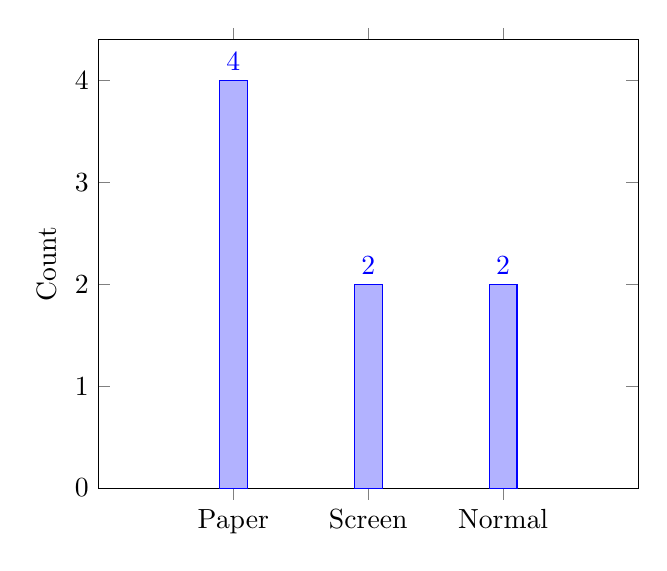
\begin{tikzpicture}
	\begin{axis}[
			ybar,
			ymin=0,
			enlarge x limits=0.5,
			legend style={at={(0.5,-0.15)},anchor=north,legend columns=-1},
			ylabel={Count},
			symbolic x coords={Paper, Screen, Normal},
			xtick=data,
			nodes near coords,
			]
      \addplot coordinates {(Paper,4) (Screen,2) (Normal,2)};
	\end{axis}
	\end{tikzpicture}
  \label{fig:preference}
  \caption{System preference}
\end{figure}

\begin{itemize}
  \item Normal paper: 2
  \item Screen: 2
  \item Pen: 4
\end{itemize}

% Usefulness and usability
\subsubsection{Usefulness and usability}

\begin{figure}[h]
  \centering
	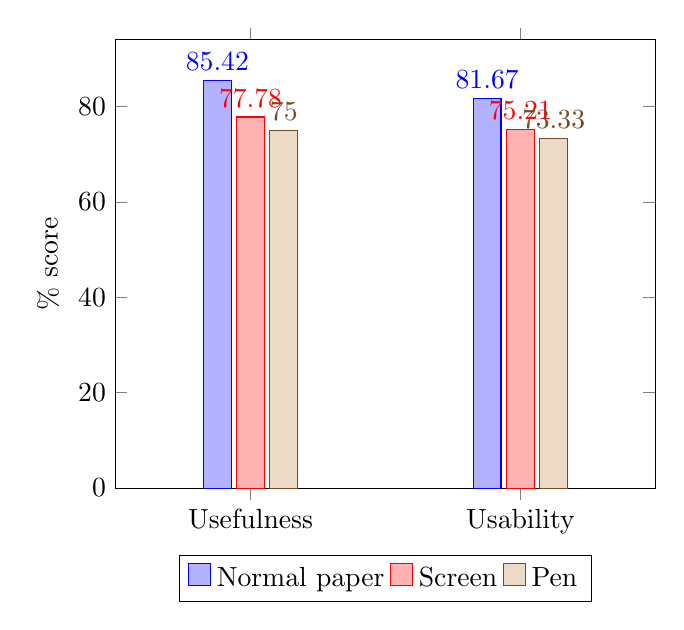
\begin{tikzpicture}
	\begin{axis}[
			ybar,
			ymin=0,
			enlarge x limits=0.5,
			legend style={at={(0.5,-0.15)},anchor=north,legend columns=-1},
			ylabel={\% score},
			symbolic x coords={Usefulness, Usability},
			xtick=data,
			nodes near coords,
			nodes near coords align={vertical},
			]
	\addplot coordinates {(Usefulness,85.42) (Usability,81.67)};
	\addplot coordinates {(Usefulness,77.78) (Usability,75.21)};
	\addplot coordinates {(Usefulness,75.00) (Usability,73.33)};
	\legend{Normal paper, Screen, Pen}
	\end{axis}
	\end{tikzpicture}
  \label{fig:usefulusable}
  \caption{Mean average scores for usefulness and usability}
\end{figure}


% Speed
\subsubsection{Speed}

\begin{figure}[h]
  \centering
  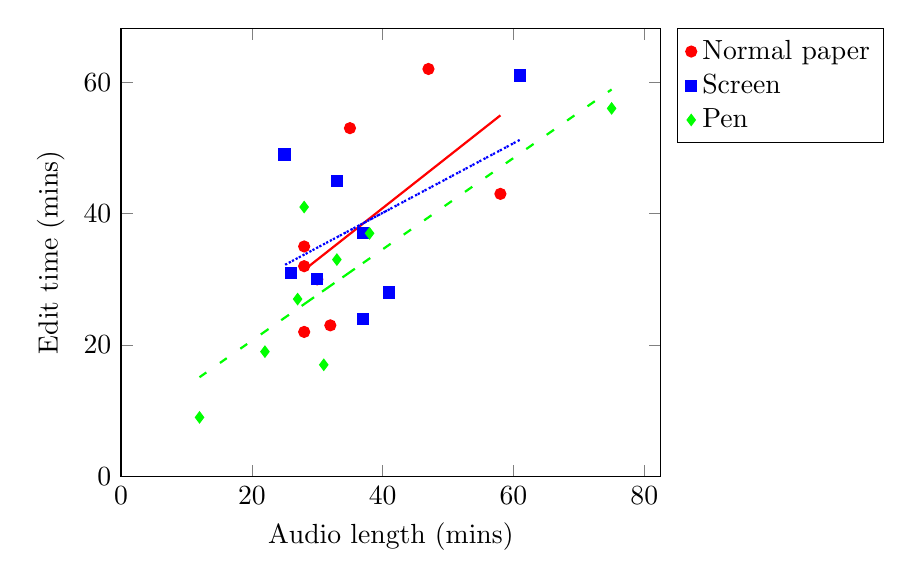
\begin{tikzpicture}
  \begin{axis}[
    legend pos=outer north east,
    legend cell align=left,
    xmin=0,
    ymin=0,
    xlabel={Audio length (mins)},
    ylabel={Edit time (mins)}]

  % NORMAL
  \pgfplotstableread{
    X Y
    30 30
    58 43
    32 23
    35 53
    28 35
    28 32
    47 62
    28 22
  }\normaltimes
  \addplot [only marks, mark = *, red] table {\normaltimes};
  \addlegendentry{Normal paper}
  \addplot [thick, red, forget plot] table[
      y={create col/linear regression={y=Y}}
  ]{\normaltimes};
  %\addlegendentry{Normal trend}

  % SCREEN
  \pgfplotstableread{
    X Y
    37 24
    61 61
    30 30
    25 49
    26 31
    41 28
    37 37
    33 45
  }\screentimes
  \addplot [only marks, mark = square*, blue] table {\screentimes};
  \addlegendentry{Screen}
  \addplot [thick, dotted, blue, forget plot] table[
      y={create col/linear regression={y=Y}}
  ]{\screentimes};
  %\addlegendentry{Screen trend}

  % PEN
  \pgfplotstableread{
    X Y
    12 9
    75 56
    31 17
    22 19
    27 27
    38 37
    33 33
    28 41
  }\pentimes
  \addplot [only marks, mark = diamond*, green] table {\pentimes};
  \addlegendentry{Pen}
  \addplot [thick, loosely dashed, green, forget plot] table[
      y={create col/linear regression={y=Y}}
  ]{\pentimes};
  %\addlegendentry{Pen trend}

  \end{axis}
  \end{tikzpicture}
  \caption{Edit time performance for each editing system, with linear regression plot}
  \label{fig:penedittime}
\end{figure}

Mean edit time, per minute of input audio:
\begin{itemize}
    \item Normal paper: 59.2 seconds (x0.9867 real-time)
    \item Screen: 59.34 seconds (x0.9890 real-time)
    \item Pen: 49.77 seconds (x0.8295 real-time)
\end{itemize}

% Usefulness


% Usability




\section{Discussion}\label{sec:paper-discussion}

\section{Conclusion}\label{sec:paper-conclusion}

\subsection{Future work}


\cleardoublepage
% !TeX root = main.tex
\chapter{Conclusions and further work}\label{chp:conclusions}

The aim of this research was to ``develop and evaluate methods for radio production that improve the production
process'' (Section~\ref{sec:aim}).  We focused our research on pre-production of speech content by professional radio
producers to make the most of the access available to us from working within the BBC.  In fulfilment of our aim, the
primary contribution of this thesis has been the development and evaluation of three methods for editing speech
recordings, through audio visualization, semantic speech editing and a digital pen interface.  We developed these
methods based on genuine requirements gathered from radio producers and evaluated them in the workplace to
ensure that our methods and results were relevant to real-life application.

To conclude this thesis, we first discuss our approach, results and contributions in
Section~\ref{sec:conclusions-discussion}, where we also reflect upon some of the tensions we observed between reading
transcripts and listening, and between paper and screen interfaces.  In Section~\ref{sec:conclusions-further}, we
describe potential options for further work, including follow-up research resulting from our studies, as well as some
broader applications of semantic audio production tools.  Finally, in Section~\ref{sec:conclusions-conclusions} we
summarise the novelties and achievements of this work.

%\section{Radio production practice}
\section{Discussion}\label{sec:conclusions-discussion}

We began our research by conducting three ethnographic case studies in the workplace to learn more about real-life
radio production practice.  We used the results to develop theoretical models of production workflows for a news
bulletin, drama and documentary.  We developed these based on direct observation of actual practice, which gave us 
insights into the genuine processes and challenges of radio production.  In addition to the workplace studies in
Chapter~\ref{chp:ethno}, we deepened our understanding of existing production workflows through interviews with twelve
radio producers as part of the user studies in Chapters~\ref{chp:screen} and \ref{chp:paper}.  These models and
insights contribute to the academic understanding of radio production practice.  The results of this ethnographic work
highlighted three directions for research involving audio visualization, textual representation of speech, and the use
of paper.  We then investigated each of these through technical intervention.

\subsection{Semantic audio visualization}

% Coloured waveform was better
Our initial investigation looked at using pseudocolour to visualize a semantic audio feature to support audio editing.
We measured the user performance for an editing task using our semantic audio visualization, compared to a normal
waveform.  The results showed that when using the semantic audio waveform, the participants completed the task faster,
with less effort and with greater accuracy than the normal waveform. This demonstrates that there is value in the
pseudocolour approach to semantic audio visualization taken by \citet{Rice2005}, \citet{Akkermans2011} and
\citet{Loviscach2011a}, which had previously been untested.

% Limited to one task, many more applications
Our experiment only focused on a single task of segmenting music from speech so there are many opportunities for
applications beyond the task we chose. Audio visualizations can either target specific tasks, or
general use that covers a range of tasks. Focusing on an individual task may produce better results, but are only suitable
for that task.  Designing a general audio visualization is much more challenging, but has the potential to create a 
greater impact as it could be used for a variety of applications.

% Chose rudimentary feature, could do better
The semantic audio visualization we designed and tested used a rudimentary semantic audio feature rather than the
state-of-the-art.  We did not attempt to create the best possible visualization as we wanted there to be an element of
human judgement in the measured task. There is potential to make better visualizations by including more and
better semantic audio features, and using more advanced methods of visualization. For example, the false colour
approach taken by \citet{Tzanetakis2000} and \citet{Mason2007} allowed multiple features to be displayed simultaneously
in a human-readable way.

% Normal waveforms not great
Although we found that users required less effort to complete the task with a normal waveform than without, they did
not complete the task significantly faster nor more accurately. We found this surprising as waveforms are widely used
throughout almost all audio editing software, so it was expected that waveforms would improve the performance of users in
completing audio editing tasks. The performance of waveforms significantly impacts the audio production community, so
this poor performance is concerning. However, this finding highlights an opportunity to increase the efficiency of
audio production software by making improvements to the waveform visualization.

\subsection{Semantic speech editing}

% can be used for pro production
We conducted two user studies in which semantic speech editing was successfully used by professional radio producers to
create real radio programmes that were subsequently broadcast. Our results support previous work in finding that
semantic speech interfaces help users navigate and edit speech \citep{Whittaker2002}, and that semantic editing is
faster than, and preferable to, using audio waveforms \citep{Whittaker2004,Sivaraman2016}. Our research went further by
conducting user evaluations in a natural working environment, and directly comparing semantic speech editing to the
existing editing workflow. This allowed us to gain insights into its limitations in the context of radio production.

The efficiency savings realised from the use of semantic speech editing tools and ASR could provide cost and time
savings over traditional editing and manual transcription.  This should free up time and budget for more valuable
production activities, which may lead to improvements in the quality of programmes and/or reduction in the cost of
production.

% ASR vs verbatim
Our semantic speech editor was similar to the system described by \citet{Rubin2013}. However, rather than using
verbatim transcripts, which are slow and expensive to produce, we used automatic speech recognition (ASR). ASR is
better suited for use in broadcast, but the erroneous transcripts it produces affect the usability of semantic editing.
Our studies revealed that the accuracy of the transcript affected the need for correction, reading speed, reliance on
listening, longevity of the transcript and the edit granularity.  Crucially, we discovered that the quality of 
modern ASR systems was sufficient to allow for semantic speech editing in radio production.  This aligns with similar
findings for the semantic editing of voice messages \citep{Whittaker2004,Sivaraman2016}.

% Only good for rough edits, but integrated with DAW
The producers we tested reported that they only found semantic editing useful for creating a ``rough edit'', where
large segments of audio are selected from the original material. This contradicts findings by \citet{Sivaraman2016} for
the editing of voice messages.
%found that for lightweight
%voice editing, users were mainly interested in using semantic editing to make fine-grain edits.  Our research showed
%that in the context of radio production, semantic editing tools were used differently.
We found that the main reason for this limitation was the lack of annotation and re-ordering features, which made it
difficult for producers to organise, structure and arrange their material in the later stages.  However, this
limitation was not an issue as our semantic speech editing tools integrated with several digital audio workstations
(DAWs), which allowed the producers to seamlessly transition to their normal tools to complete their production.

%seamlessly move from our tools to their normal editing
%software, so that they could use semantic editing tools to create a rough edit, then

%by exporting an edit decision list
%(EDL) that described the producer's edits. This allowed for a non-destructive integration where edits could be undone.

% correction
We tested a variety of additional features to support semantic editing, including transcript correction and confidence
shading.
%TODO and speaker diarization.
We found that many of the transcript errors encountered were specific to the
programme content, such as names and topic-specific words.  However, most producers were only interested in correcting
errors that were particularly distracting.  Most producers we tested found confidence shading to be useful overall,
which supports \citet{Burke2006}, but contradicts \citet{Suhm2001} and \citet{Vemuri2004}.

%Both semantic speech editors included confidence shading, which low-lighted or underlined words that the ASR was not
%confident were correct.


% APPLICATIONS


%Radio producers often work to tight unmovable deadlines, and have a small and shrinking budget.
%This extra time could be
%spent on more valuable activities such as research and recruitment of interviewees, which may improve the overall
%quality of the final programme. Alternatively, these efficiencies could be used to reduce the cost of production whilst
%retaining the same quality of output.

DAWs are powerful, feature-rich tools, but to novice users they can be intimidating to work with.  Semantic speech
editing tools are easier to use and more accessible than waveform-based tools \citep{Yoon2014,Sivaraman2016}.
Podcasting has already democratised the distribution of audio content, and semantic speech editing may have the
potential to achieve something similar for audio production. This would allow more people to access audio production,
which would hopefully lead to the production of more and better audio content.

Alternative methods of interacting with audio content may also give rise to new creative opportunities for more
innovative programme making.  For example, the comedy duo known as ``Cassetteboy'' \citep{Perraudin2014} patiently
trawl through hours of video footage to re-order the words of famous speeches in amusing ways, which could be achieved
much more easily using a semantic speech editor.

%Semantic speech editing provides an alternative to audio waveforms for interacting with speech content. Text-based
%interfaces allow users to quickly search and discover content. This may open up new possibilities for different types
%of content that were not previously possible when using waveforms. For example, the comedy duo ``Cassetteboy'' remix
%speech content of popular figures to change the content in radical ways, such as turning political speeches into rap
%songs. Doing this manually requires huge amounts of patience and time to edit, but could be achieved relatively quickly
%using a semantic speech editor.

\subsection{Reading vs listening}

% Limitations of transcripts
Transcripts display the words that were spoken in a recording, but much of the content's true meaning is hidden in the
audio. Although transcripts show \textit{what} was said, they do not reveal \textit{how} it was said, which is crucial
when producing radio programmes.  As one producer pointed out, ``radio is made with your ears''.

% reasons for listening
The only way to fully comprehend audio recordings is through listening.  We found that radio producers used listening
to process information, judge the quality of the sound and identify non-speech sounds.  Some producers reported that
reading and listening at the same time enabled them to comprehend information more easily, supporting the findings from
\citet{Vemuri2004}.  Producers listened to identify any low quality audio, such as ``umm''s and ``err''s, and long or heavy
breaths. These are visible in verbatim transcripts, as used by \citet{Berthouzoz2012} and \citet{Rubin2013}, but are
not included in ASR transcripts.  Producers also listened to identify any high quality moments that may not be
identifiable using the transcript, and non-speech sounds that they might want to include or exclude in their programme.


% not listening while logging
The existing radio production workflow involves producers ``logging'' recordings by listening to the audio and typing
rough quotes and labels.  This process is time-consuming and tedious, but it helps the producer to review and organise
their content.  ASR transcription replaces this logging process, which saves producers time and effort. However, it
also means that producers don't have to listen to the audio before editing, which may prevent some producers from
reviewing the material before making editorial decisions.  There is a risk that over-reliance on transcripts may mean
missing out on good quality content or not avoiding poor quality content, which would affect the overall programme
quality.

%Some of the producers in the Chapter 5 study
%said they valued this listening opportunity, and one of the producers in Chapter 6 wanted to listen back in full first.

% integrated playback
Providing an easy way to listen to the audio underlying the transcript is important. Our screen-based semantic speech
editor included integrated playback, which allowed users to navigate the audio using the text.  Time compression, such
as described in Section 2.6, would also allow producers to listen faster, and producers valued this feature when we
added it to our screen-based editor following user feedback. Reading the transcript while listening also increases the
speed at which time-compressed audio can be comprehended \citep{Vemuri2004}.

% transcripts not always needed
However, we found that in some situations, transcripts are not necessary or useful. With short recordings of less than
15-25 mins, producers reported that they can remember what was said and when, and some programmes have a greater focus
on the sound design, which limits the value of a transcript.

%However, our paper-based
%editor did not, which meant that users did not cope well with low accuracy transcript.

% use of time compression

We found that transcripts are not normally published due to the high cost of creating verbatim transcripts.  ASR and
transcript correction tools could make it possible for producers to create a verbatim transcript as part of their
production process.  Publishing these could allow audio content to be more easily searchable and discoverable through
Internet search engines, for example.  Word-level timings could also be used to link directly to segments of audio. For
example, NPR's online clipping tool ``Shortcut'' \citep{Friedhoff2016} allows radio listeners to create a short clip
from a radio programme and share it with their friends. 

\subsection{Paper vs screen}

Our workplace studies identified that many radio producers enjoy working with paper.  Our user study in
Chapter~\ref{chp:screen} also found that many producers want to be able to work away from their screens.  This led us
to develop a novel semantic speech editing system that used digital pens to allow producers to edit speech recordings
using a paper transcript.  We conducted a qualitative user study of professional radio producers that compared our
paper interface to a screen-based semantic speech editor. The results of our study provide insights into the relative
benefits of editing speech on paper compared to screens. We found that both the paper and screen interfaces worked
well, but that each had advantages and disadvantages in different contexts.

% summary
Overall, we found that the paper interface was better suited to quick and simple edits where listening is not as
critical, such as with high accuracy transcripts, or very recent recordings.  Our screen-based semantic speech editor
included integrated playback and correction features, which made it better for more complex editing with less familiar
audio and less accurate transcripts.

% benefits of paper
Producers reported that paper transcripts were easier to read and remember, and made it easier for them to think widely
and orientate themselves.  They reported that our digital pen interface was simple, intuitive, precise and allowed edit
decisions to be made quickly and easily.  However, producers had concerns over the cost of an additional device which
would likely have to be shared amongst a team, and because they were worried about losing it.
%TODO Why is sharing a problem?

% portability
The physical nature of the digital pen and paper made it better suited to travel and working away from the desk. This
gives producers greater flexibility to work in more comfortable locations and while commuting.  However the digital pen
interface uses considerable amounts of paper, involves carrying a digital pen, and requires access to a colour laser
printer, which would make it difficult to work ``on the road''.  The screen interface could be used on a
laptop or tablet, which have the added benefit of integrated playback, but screens are heavier, bulkier and have a much
shorter battery life than digital pens.

% collaboration
Radio is usually produced by a team, so tools that facilitate collaboration are important to working in such an
environment.  We found that the physicality and pagination of paper made it better suited to face-to-face collaboration
than the screen. However, the screen interface is capable of remote collaboration, and could be used over the Internet
for real-time collaborative speech editing.

% implementation limitations - integrated playback, correction, undo
The limitations of the digital pen system we used prevented us from including features for integrated playback,
correction and undo. The lack of integrated playback forced producers to replay and navigate audio using a separate
device, which made it more challenging to interpret errors in the transcript. This was more of an issue with low
quality transcripts, which could also not be corrected using the digital pen.  The integrated playback of the screen
interface made it easier for the participants to find and fix mistakes in the transcript.  This also made it
easier to edit content that required more listening, such as old or unfamiliar recordings.

%Our system interpreted the user's gestures strictly, which created a source for unintentional errors.

%\section{Applications}


%The recent release and investment in the Descript editor demonstrates that there is increasing commercial interest in
%semantic speech editing for audio production. Avid have included their ScriptSync tool since 2007(?) and released a
%major update in 2016(?). This shows that there is market demand for timed transcript tools and semantic speech editing
%in the audio production community.



%=====================================================================================================================

% CHAPTER INTRO


% Release the structure of the chapters

%=====================================================================================================================

% RE-INTRODUCTION
%   - an introductory restatement of research problem, aims and/or research question
%   - restate the objectives


% APPROACH - how and why - justify the approach adopted

%To achieve this aim, we started by conducting three ethnographic case studies to investigate how radio production is
%currently conducted at the BBC. This helped us to ensure that the direction of the research was aligned with the
%real-life challenges faced by professional producers.  This investigation provided three directions for the research,
%each of which we investigated in turn.

%Previous work had used audio visualization techniques to display more information about audio signals, but they had not
%attempted to measure the effect these visualizations had on production tasks.
%We conducted a quantitative study that measured the actual and reported performance of users in segmenting music from
%speech using different audio visualizations.
%This allowed us to demonstrate the measurable effect that waveforms and a simple semantic audio visualization had on
%user performance of a typical radio production task.

%Semantic speech interfaces had been considered by previous research as an alternative method of navigating and
%editing speech content.
%These systems did not attempt to measure user performance, and most used perfect transcripts which are too expensive to
%produce in professional production. \citet{Whittaker2004} showed that ASR transcripts could be used for editing.
%We developed a semantic speech editor that integrated with the BBC's radio production systems, which allowed us to
%evaluate semantic editing in a professional context.
%We then evaluated our system on radio producers who used it to produce programmes for broadcast, and compared our
%system to the existing workflow.

%Finally, we identified an opportunity to develop a novel interface that used paper transcripts to edit speech content.
%We worked directly with professional producers to refine an early prototype, then collaborated with a digital pen
%manufacturer to create a working system.
%We evaluated our system for use in real-life programme-making, and compared it to our screen-based semantic speech
%editor, and an inactive paper transcript.

% TAKE-HOME MESSAGE - highlight the ‘take-home message’ 

%Professional radio production can benefit from semantic audio tools

%We demonstrated three approaches in which semantic audio can be used to make professional radio production more
%efficient

%Audio visualization and semantic speech editing have benefits to professional radio production




% SUMMARY
%   - a summary of findings and limitations
%   - Summarize what was said in the different chapters
%   - include the most important points already covered

%Chapter~\ref{chp:ethno} used ethnographic case studies to investigate audio editing workflows for the production of a
%news bulletin, drama and documentary within BBC Radio. Our investigation identified three themes regarding audio
%waveforms, textual representaton and the use of paper.

%- Audio waveforms are widely used
%- Producers work with textual representation
%- Drama and docs producers use paper

%Chapter~\ref{chp:colourised}:

% Audio visualization
% - previous systems had not been formally evaluated
% - Using semantic audio to add colour to waveform improves performance for music/speech segmentation
% - Faster, more accurately and with less effort
% - our study demonstrates pseudocolour approach by Rice2005, Akkermans2011 and Loviscach2011a has value
% - false colour from Tzanetakis2000 and Mason2007 may have greater benefits

%- Normal waveform was not significantly faster, nor more accurate
%- We chose task-specific, but alternative could be general
%- We only focussed on one task. Audio visualization has applications beyond music/speech segmentation, such as
%  programme segmentation, spotting noises


%Chapter~\ref{chp:screen}:

%- Semantic speech editing can be used for professional radio production (continued to use)
% - Whittaker2004 found that semantic editing of voicemail messages was faster than editing with a waveform. Our
%   research supports this, and shows that it also applies to professional radio production
% - Sivaraman2016 found semantic editing was good enough to replace waveform editing and more accessible

%- The goal of our system was similar to Rubin2013, but used ASR, integrated with radio production system and was evaluated
%- Annotation is needed to organise and structure content
%- Collaboration is useful
%- Portability allows flexible working away from desk
%- Does working with text affect the final result? Could have negative impact, could open up creative possibilities

% radio is made with your ears
% - text can only represent the words that were spoken, which only tells half the story
% - semantic editing can't fully repace it
% - combination with listening features such as time compression could help

%- Listening is important
% - limits usefulness of semantic speech editing
% - Whittaker2002 found that users could use stratigic fixation to scan transcripts to extract info and judge
%   relevance without listening. We found similar, but listening is still required.

% faster playback
% - Can use time compression (section 2.6), which works even better with transcript
% - Whittaker2002 included it
% - Vemuri2004 shows that adding transcripts increases maxiumum playback rate

% confidence shading
% - Suhm2001 found that confidence shading slowed down correction
% - Burke2006 reported that users find confidence shading helpful
% - Vemuri2004 found no statistically significant difference in comprehension with/without confidence shading

% transcript accuracy
%- Transcripts are sufficiently accurate for professional radio producton
% - ASR is sufficiently accurate for professional production
% - Yoon2014 found that transcripts were not accurate enough to use without listening
% - Sivaraman2016 found semantic editing ASR errors weren't a heavy distraction

%One of the findings from Chapter~\ref{chp:ethno} was that the observed radio producers used paper to allow for
%handwritten annotation and to facilitate face-to-face collaboration.
%Chapter~\ref{chp:paper}:
%- Screen and digital pen interfaces both work well for semantic speech editing, strengths in different situations
%- Paper is easier to read and simpler, making it better for simple edits with accurate transcripts
%- Screen has integrated playback and correction, which is better for complex editing and less accurate transcripts
%- Screen interface has remote collaboration, but pen might be better for face-to-face
%- Pen has greater flexiblity for portablity, but depends on access to printer
%- Lack of re-ordering and labelling in both mean it's only useful for rough editing

%- Transcripts not needed for short recordings, or where content is led by sound
% - short recordings can be kept in memory (15-25 mins)
% - actuality led programmes, emphasis on sound

% stage of usefulness
% - mostly useful for rough edit
% - continuing to further stages requires good integration with tools
% - EDL allows non-destructive integration 


%- Participants reported that using paper made it easier to read transcripts, remember information, think widely and
%  orient themselves. This aligns with previous research.

% - Editing with pen better for making simple edits and quick decisions, using familiar content with high-quality transcript
% - Editing with screen better for more complicated editing involving complex decisions using less familiar content
%   with a lower accuracy transcript
% - Collaboration - pen better for face-to-face, screen allows remote collab
% - Portability - pen is more flexible, allowing for working in more places away from screen, but relies on printer
% - Labelling and re-ordering features would be useful
% - Listened to process information, judge quality and identify non-speech sounds

% - Transcript accuracy affected need for correction, reading speed, reliance on listening, longevity and edit
%   granularity
% - Sivaraman2016 found that users only made fine-grain edits rather than rough edits



% LEARNINGS
%   - What do I know now, that I didn’t know before doing the research?
%   - What do I know that no one else knows? (e.g., things that arise from my unique context or data sets)


% COMPARE TO EXISTING WORK
%   - new research, positioned against existing knowledge
%   - Does your work confirm or contradict other published work?
%   - key aspects of the literature you have studied and say how they are justified or contradicted by your research


% LIMITATIONS
%   - stress the limitations of the current work


% CONTRIBUTIONS
%   - Give an overview of the main original contributions
%   - emphasise the contribution that it makes to research

  %A set of theoretical models of audio editing workflows in professional radio production, which
  %contribute to the academic understanding of radio production.

  %A demonstration of the feasibility of semantic audio visualization, and insights into the
  %effectiveness of audio waveforms, for segmenting music from speech.

  %The application of semantic speech editing to professional radio production, with
  %demonstration of its feasibility and insights into its limitations. 

  %A novel approach to editing speech recordings through the combination of semantic speech
  %editing and a digital pen interface. Insights into the relative benefits of paper and screen interfaces for semantic
  %speech editing.

  %Other outputs include: contributions towards the academic understanding of radio production workflows
  %and open-source implementations of tools for semantic speech editing and audio visualiation (see
  %Appendix~\ref{app:tech}).

% APPLICATIONS
%   - Who cares? / Who should care?
%   - Practical applications/implications
%   - a paragraph in which you reflect upon the practical implications of your results into the your field
%   - connect the dots in an attempt to lead the reader to a deeper understanding of the implications of the work

  % benefits and drawbacks of automation
  % - logging and cross-referencing could be assisted or automated
  % - this may remove the opportunity to listen back, which help thinking process
  % - serendipidy may play an important role in identifying high quality content

  % commercial interest
  % - Investment in Descript shows that there is market interest and value in semantic speech editing
  % - Avid have included ScriptSync since 2007

  % free up time/money
  %Radio producers have tight deadlines and reducing budgets. Tools which allow them to be more efficient can therefore
  %free up time and creative energy to improve the output of the programme.

  % enabling new types of programmes
  %Alternative methods of interacting with audio content may also give rise to opportunities for more innovative programme
  %making.
  %For example, the comedy duo known as ``Cassetteboy'' \citep{Perraudin2014} remix speeches to make popular figures say
  %controverial things, which could be achieved very easily using a semantic speech editor.
  % could be misused?

  % democratisation
  %Semantic editing tools may lower the barrier of entry to audio production.
  %Podcasting had democratized distribution of audio content, but digitial audio workstations are feature-rich
  %and have complicated layouts, which may be intimidating to novice users.
  %Semantic speech editors could make it easier for amateur users to create their own content, and the increasing
  %popularity in podcasts gives amateur producers an audience and method of distribution.
  % - Sivaraman2016 found semantic editing was more accessible than waveform editing
  % - Yoon2014 found that semantic editing was easy to use

  % correction could allow publication of transcripts
  % - correcton is less necessary when producer can remember what happened
  % - accuracy affects longevity of recordings as memory fades
  % - accuracy may affect granularity
  %NPR Shortcut\citet{Friedhoff2016}


% FURTHER WORK
%   - What questions does your research raise, and is there potential for further research?
%   - Recommendations for further research


%=====================================================================================================================


%It would likely be easier to create effective specific visualizations as they
%only need to include information relevant to the application, but this would make it difficult to cater for every
%possible use case. Users would also have to switch between multiple specific visualizations depending on the task they
%are performing, and learn how to read each of them. General visualizations would have to contain information relevant
%to all applications. It would be difficult to select the most relevant information and map it in a way that humans can
%easily interpret. However, they could be used for any purpose without users having to switch between or learn to read
%multiple visualizations.






\section{Further work}\label{sec:conclusions-further}

Further work that could follow on from the research of this thesis includes:

\paragraph{Collaborative semantic speech interaction:}
% use operational transformation to allow simultaneous access and editing
% NPR presedential debate fact-checking \citep{Fisher2016}

The semantic speech editing systems we developed during this thesis were designed to be operated by individuals.
However, as shown in Chapter~\ref{chp:ethno}, radio production involves teams of people.  Collaborative tools may help
these teams work together more efficiently.  Operational transformation techniques \citep{Sun2004} have enabled the
development of collaborative document editing tools, such as the popular Google Docs, which can facilitate concurrent
team-based working.  For example, \citet{Fisher2016} describes how NPR used Google Docs to enable over a dozen
producers to collaboratively fact-check the US Presidential Election debates live, using real-time ASR transcripts. By
linking the text to audio, a similar approach could be used for collaborative semantic editing of speech. Teams could
also use annotation to make suggestions for edits that are then accepted or rejected by the programme producer.
%TODO Integrated writing and editing, like Shin2016

\paragraph{Assisted/automatic de-umming:}
% take into account intonation

In Section~\ref{sec:doc}, we saw that a large proportion of a studio manager's time was spent on cleaning-up interview
material by removing unwanted vocal noises, known as ``de-umming''. Examples of unwanted noises include ``umm''s and
``err''s, long or loud breaths, and redundant phrases such as ``you know''.  These can be difficult to identify, as
their presence is not clearly visible using current tools, and they can be difficult to remove as they often overlap
and blend with the speech. \citet{Loviscach2013} demonstrated a prototype ``umm detector'' that extracted MFCC
\citep{Imai1983} features from the audio and used template matching to visually highlight potential ``umm''s. We could
not find any other work that attempted to detect or remove unwanted speech noises.

One solution could be to train an
ASR system to ``transcribe'' unwanted sounds. These ``words'' could then be highlighted, or removed in the same way
that transcripts can be semantically edited.  However, this assumes that these noises have clearly defined boundaries,
which they often do not.  In our experience, de-umming involves a level of editorial and creative judgement, so a
interface that supports a human-in-the-loop system may be necessary.
% - Rubin2013 and Berthouzoz2012 included de-umm features

\paragraph{Improved automatic speech recognition:}
% use prior information to produce better transcripts

In this thesis, we found that the transcripts produced by current ASR systems were sufficiently accurate to perform
semantic speech editing in professional radio production. However, as discussed in
Section~\ref{sec:transcript-generation}, ASR quality affects comprehension, search, and the need for correction, so it
is desirable to improve the transcript accuracy. Prior to transcription, much is already known about the content of the
speech, and by providing this information to the ASR system in advance, it could be used to improve the quality of the
transcript.  For example, the topic of conversation could be used to weight the likelihood of words related to that
topic appearing.  Many ASR systems have a speaker diarization pre-processing stage, and the number, gender and identity
of speakers could also be used to inform this process.

\paragraph{Improved digital pen system:}
% re-ordering and labelling
% integrated playback using wireless link
% correction
% better intepretation

The design of our digital pen semantic editor in Chapter~\ref{chp:paper} was influenced by the technical limitations of
the technology that we used to implement it.  This prevented us from including certain features such as integrated
listening and correction, and was inflexible in interpreting the user's gestures.  These issues could be solved by
using a different system for implementation.

The digital pen we used operated in batch mode as it connected to the
computer using a USB dock. This prevented us from integrating control over the playback of the audio. A digital pen
with a wireless link could allow a user to play, pause and navigate the audio using the paper transcript.  The design
of our paper layout used strict rectangular boundaries to capture edit commands, which created a potential source of
errors. By using a more flexible approach, the system may be able to better understand the user's intentions and avoid
inadvertent mistakes.  Additionally, the ability to distinguish between edit commands and handwriting could allow the
user to both edit and correct the transcript on paper.

\paragraph{Penless paper editor:}
% use scanner or camera, mask out printed area
% digital ink with electronic paper

In Chapter~\ref{chp:paper}, we based the design of our system on a digital pen as it combined the readability of real
paper with the digital capture of freehand annotations. However, when we evaluated the system, some producers were
concerned about losing the pen, having to share it and its cost. Several producers said they would prefer to use a
highlighter or different coloured ink, which digital pens do not support. There are also patents that cover digital
pens \citep{Fahraeus2003}, which can make development more difficult.

Scanners and cameras could be used as alternative methods of digitally capturing freehand annotations from paper.  For
example, a barcode or QR code could be used to label each page with a unique identity that links to a stored image of
the printed page. The stored image could be used to mask the picture/scan of the paper, leaving only the user's
annotations. Image analysis could then be used to interpret the user's annotations and translate them into edits,
corrections and labels.
%TODO E-paper interface

\paragraph{Rich audio visualization:}
% multiple features
% different colour spaces
% texture

In Chapter~\ref{chp:colourised}, we showed that speech/music segmentation can be performed faster, more easily and more
accurately by using pseudocolour to map a semantic audio scalar feature to a colour gradient. Previous systems from
\citet{Tzanetakis2000} and \citet{Mason2007} have also showed how false colour can be used to map multiple features to
colour space.  Onomatopoeia is the formation of words that resemble the sound they describe.  The author believes that
there is significant untapped potential to design an onomatopoeic audio visualization that ``looks like it sounds''.
Such a visualization could provide an efficient and accessible way of navigating all types of audio content.

Crossmodal correspondences could be exploited when designing the mapping between semantic audio features and visual
properties.  Many of the links listed in Section~\ref{sec:crossmodality} have yet to be tested for visually navigating
audio content, and previous work on audio visualization has mostly focused on colour.  Other visual properties such as
shape and texture could be used to increase the richness of the information presented in the image.  For example,
textures can be generated using procedural techniques \citep{Ebert1994}, which allows them to be synthesised from
semantic audio features.  However, selecting the best combination of semantic audio features and visual mappings is a
huge challenge, and is likely to be different for each task and signal.

%\paragraph{Cost/benefit of transcripts:}
%We found that semantic editing was faster for long recordings, but it would be
%interesting to investigate how long a recording needs to be before the benefits of semantic editing outweigh the
%costs.  Additionally, it is unclear how much of the speed benefit comes from automatically generating the transcript,
%and how much comes from the editing interface.

%\paragraph{Non-speech sounds}
%Tagging music and environmental sounds

\paragraph{Application to television}

The focus of research in this thesis has been solely on semantic audio tools for the production of radio. However,
there may be opportunities to transfer some of the tools and findings from this work to the production of television.
The weekly reach and consumption hours for television (91\%, 25 hours) is similar to that of radio (90\%, 21 hours)
\citep[pp.  82, 119]{Ofcom2017}.  However, based on the author's experience in working with BBC producers on both sides
of the fence, there are big differences between production in television and radio in terms of team size, budget and
culture. These differences may impact on the relevance of the work.

Radio is often produced by small teams of between two and five. Television production involves dozens or sometimes
hundreds of people, as demonstrated by the list of credits at the end of each programme.  In 2016/17, the BBC spent
\textsterling2.48B on television production -- over five times the amount that was spent on radio production \citep[pp.
39, 111]{Ofcom2017}. There are also important cultural differences between television and radio production. For
example, in the BBC radio producers are employed directly by the public service arm of the BBC as full-time staff. In
television, most producers are freelancers working on short-term contracts, either for an independent company or a
commercial arm of the BBC. It is likely that these differences will affect the effect and use of semantic audio
production tools, but this is currently unknown, so may be an interesting direction for the research.


% SPEAKER DIARIZATION 
%All of productions we observed may benefit from being able to see where different people are speaking in a recording,
%known as ``speaker diarization''. In drama, it could help producers identify different lines in the script, in
%documentaries it could highlight the position of the questions in interview recordings, and in news it could help
%producers navigate long off-air recordings. There is an existing body of work on speaker diarization
%\citep{AngueraMiro2012} that has been used to help users navigate radio archives \citep{Raimond2014}, but could also be
%used in the production process.

% PRE-RECORDED CONTENT
%Drama production involves recording multiple takes of the same content. This technique allows producers to get the most
%from the actors, but means that it can be difficult to select which performances to use.  Comparing takes during
%post-production is a manual and inefficient process.  Providing an easy way to directly compare performances could
%allow the director to make a better informed decision on which takes to use. Automatically aligning the takes on
%different tracks in the DAW would be an easy way to make such comparisons.


\clearpage
\section{Summary}\label{sec:conclusions-conclusions}

%New methods for the analysis of audio production workflows.
%A set of novel theoretical models of audio editing workflows that contribute to the academic understanding of
%professional radio production.

%The first formal study on the effect of audio waveforms and semantic audio visualization on user performance.
%Insights into the effectiveness of audio waveforms, for segmenting music from speech.

%The first application of semantic speech editing to professional radio production. Development of a semantic speech
%editor that includes a novel DAW integration. The first formal user study of semantic speech editing for audio
%production. Insights into the challenges and limitations of semantic speech editing in the context of radio
%production. 

%A novel approach to editing speech recordings through the combination of semantic speech editing and a digital pen
%interface. Insights into the relative benefits of paper and screen interfaces for semantic speech editing.

We started our research by conducted three ethnographic case studies of professional radio production. We found that
the radio producers used audio waveforms and textual representations to navigate and edit audio content, and used paper
to make freehand annotations and facilitate face-to-face collaboration.  Based on these findings, we developed and
evaluated three semantic audio tools for radio production using audio visualization, and semantic speech editing on 
screen and paper interfaces.

We developed a simple semantic audio visualization for segmenting music from speech and conducted the first formal
study on the effect of audio waveforms and semantic audio visualization on user performance. We found that our semantic
audio visualization was faster, more accurate and required less effort than using a waveform.  Using an audio waveform
required less effort than no visualization, but was not significantly faster, nor more accurate.

We developed a semantic speech editing system for radio production, and evaluated this approach with professional radio
producers for the production of genuine programmes. The radio producers were successful in using semantic speech
editing with ASR transcripts as part of their workflow, and continued to use our system after the study. Through our
study, we also gained insights into the importance of annotation, collaboration, portability and listening.

Finally, we designed and developed a novel system for semantic speech editing on paper using a digital pen. We compared
our paper interface to a screen interface and normal paper through a user study of professional radio producers. We
found that the benefits of reading from paper and the simplicity of the pen interface made it better for fast, simple
editing with familiar audio and accurate transcripts.  The integrated listening and correction features of the screen
interface made it better for more complex editing with less familiar audio and less accurate transcripts.  We also
gained insights into effect of ASR accuracy, the role of listening, and the relative benefits of paper and screen
interfaces for collaboration and portability.

%In this thesis, we have demonstrated three successful approaches to improving radio production.



\begin{appendices}
  \renewcommand\chaptername{Appendix}
  \cleardoublepage
  % !TeX root = main.tex
\chapter{Technological developments}\label{app:tech}

\section{Dialogger}\label{sec:dialogger}

\texttt{https://github.com/bbc/dialogger}

\begin{figure}[h]
\centering
  \includegraphics[width=\columnwidth]{figs/dialogger-flow-diagram.png}
  \caption{Flow diagram of the Dialogger system. Excluded components are shown in red.}
  \label{fig:dialogger-flow}
\end{figure}

Made a screen-based semantic speech editor. Here's how it works.

\clearpage
\section{Vampeyer}\label{sec:vampeyer}
The direction of the research in this project centres around turning audio data into image data. There is already some
software that visualizes audio and audio features in a number of ways, notably Sonic Visualiser \citep{Cannam2010}.
However, the visualization algorithms are always hard-coded into the program, making prototyping of new methods
prohibitively difficult.

\subsection{Design}
A system of software was developed for visualizing audio in order to allow flexibility while maintaining consist inputs
and outputs. It was designed to expand on existing systems for audio analysis so to avoid duplication of effort and to
allow modularisation of algorithms.

The system was developed as a plugin framework with clearly defined inputs and outputs. It is based on the existing
Vamp plugin framework, developed by Queen Mary University of London \citep{Cannam2010}, which analyses audio data and
outputs frame-- or time-based features. The visualization plugin is designed to take these features and produce a
bitmap image. An outline of the system design is shown in Figure~\ref{fig:vampeyer}.

\begin{figure}[ht]
  \centering
  \includegraphics[width=0.8\textwidth]{figs/vampeyer.pdf}
  \caption{High-level system diagram of the Vampeyer visualization framework}
  \label{fig:vampeyer}
\end{figure}

The visualization plugin defines which Vamp plugin outputs it requires, including the block/step size and parameters.
At least one Vamp plugin is required, but there is no restriction of the number of different Vamp plugins that can be
used.

Both frameworks are written in C++ which allows for a fast processing time.  This is important for situations where
audio has to be processed on-the-fly, such as for exploring an archive without having to pre-process everything in it.
The plugins are compiled into shared libraries, so they can easily be distributed without users having to recompile
locally and integrated into third-party software.

\subsection{Implementation}
A C++ header file was created which implements the design.  Five data structures are also defined which define how data
should be sent and returned from the functions.

{\singlespacing
\begin{itemize}
  \item \texttt{VampParameter} is a name/value pair used to store a parameter
  \item \texttt{VampParameterList} is a vector of \texttt{VampParameter}s
  \item \texttt{VampPlugin} stores the name of a Vamp plugin along with a\\
    \texttt{VampParameterList} and the preferred block and step sizes
  \item \texttt{VampOutput} stores a \texttt{VampPlugin} and output name
  \item \texttt{VampOutputList} is a vector of \texttt{VampOutput}s
\end{itemize}
}

Two primary functions are used to define the input audio features and their conversion to a bitmap.

\begin{itemize}
  \item \texttt{getVampPlugins} returns a \texttt{VampOutputList} variable that contains a list of Vamp plugin outputs
    which must be provided as input
  \item \texttt{ARGB} takes the Vamp plugin output data as a \texttt{Vamp::FeatureSet} variable, the sample rate of the
    audio and the desired width and height. It returns a bitmap image formatted in 32-bit ARGB format (alpha, red,
    green, blue).
\end{itemize}

A number of example plugins were written to demonstrate the capabilities of this approach, and to act as useful pieces
of software in their own right.  These include a standard waveform, waveform colourised by low energy ratio (see
Section~\ref{sec:studywaveform}), waveform colourised by spectral centroid (identical to Freesound) and an MFCC grid
visualization with waveform overlay.

The plugins need to be run by a host program which reads the audio data, processes it using the Vamp plugins, sends
their output to the visualization plugin and then writes the image data. Such a program was written as a command-line
tool that can either display the image in a window or write it to disk as a PNG-encoded file. This makes it useful for
both prototyping and for back-end processing on a server, for example.

\clearpage
\section{BeatMap}\label{sec:beatmap}


\end{appendices}

\cleardoublepage
\fancyhead[LO]{\leftmark}
\fancyhead[RE]{\rightmark}
\printbibliography

\end{document}
